\chapter{PHÂN TÍCH ĐẶC ĐIỂM DỮ LIỆU QUA THỐNG KÊ VÀ TRỰC QUAN HÓA}

\startcontents[chapters]
\printmyminitoc{
Chương này là phần thực hành trọng tâm của báo cáo: dữ liệu đã thu thập ở Chương 2 được phân loại biến, thống kê mô tả, trực quan hóa và so sánh trước--sau tiền xử lý. Nội dung bám theo yêu cầu trong \texttt{docments/chuong\_4.md}: nhóm A và B phải chọn tối thiểu 5 biến cho mỗi bộ dữ liệu; nhóm B phải thể hiện đặc thù chuỗi thời gian/cảm biến; nhóm C phải số hóa dữ liệu đa phương tiện thành đặc trưng Quantitative trước khi thống kê. Ngoài biểu đồ tạo bằng Python, chương còn đối chiếu một số biểu đồ tương ứng được tạo trong Excel để chứng minh tính nhất quán của kết quả.}

\section*{Quy trình phân tích và bản đồ minh chứng}

Mỗi bộ dữ liệu trong chương được xử lý theo bốn bước thống nhất:

\begingroup
\setlength{\parindent}{0pt}
\setlength{\parskip}{0.75\baselineskip}

\textbf{Bước 1. Phân loại bản chất biến:} xác định biến Qualitative hay Quantitative; với biến Quantitative, phân biệt Discrete và Continuous.

\textbf{Bước 2. Lập bảng tần suất và thống kê mô tả:} biến Qualitative dùng tần suất, tần suất tương đối và mode; biến Quantitative dùng mean, median, mode, percentile, range, variance, standard deviation, coefficient of variation (CV) và interquartile range (IQR).

\textbf{Bước 3. Trực quan hóa:} nhóm A dùng histogram, boxplot, scatter plot, bar/pie chart; nhóm B dùng thêm line chart để đọc xu hướng và mùa vụ; nhóm C dùng các biểu đồ theo đặc trưng đã số hóa.

\textbf{Bước 4. So sánh trước--sau tiền xử lý:} đặt dữ liệu thô cạnh dữ liệu sạch để đánh giá tác động của điền khuyết, xử lý ngoại lai, chuẩn hóa, log-transform, differencing hoặc nội suy theo thời gian.
\endgroup

\begin{table}[H]
\centering
\vspace*{1.2\baselineskip}
\caption{Bản đồ minh chứng dùng trong Chương 4}
\label{tab:ch4_artifact_map}
\footnotesize
\setlength{\tabcolsep}{2pt}
\renewcommand{\arraystretch}{1.22}
\begin{tabularx}{\textwidth}{>{\RaggedRight\arraybackslash}p{0.16\textwidth}>{\RaggedRight\arraybackslash}p{0.27\textwidth}>{\RaggedRight\arraybackslash}p{0.37\textwidth}Y}
\toprule
Hạng mục & Source code & Output chính & Vai trò \\
\midrule
Heart Disease & \path{src/analyze_heart_disease.py} & \path{outputs/tables/heart_disease_*.csv} & Nhóm A, minh họa đầy đủ 4 bước \\
CDC Diabetes & \path{src/analyze_cdc_diabetes.py} & \path{outputs/tables/cdc_diabetes_*.csv} & Nhóm A, dữ liệu lớn và mất cân bằng lớp \\
Breast Cancer & \path{src/analyze_tabular_health.py} & \path{outputs/tables/breast_cancer_*.csv} & Nhóm A, biến y khoa có lực phân tách cao \\
Appliances Energy & \path{src/analyze_appliances_energy.py} & \path{outputs/tables/appliances_energy_*.csv} & Nhóm B, chuỗi thời gian hồi quy \\
HAR và MHEALTH & \path{src/analyze_har.py}; \path{src/analyze_mhealth.py} & \path{outputs/tables/har_*.csv}; \path{outputs/tables/mhealth_*.csv} & Nhóm B, chuỗi cảm biến \\
HAM10000 & \path{src/analyze_ham10000.py} & \path{outputs/tables/ham10000_*.csv} & Nhóm C, ảnh \\
Reuters-21578 & \path{src/analyze_reuters.py} & \path{outputs/tables/reuters_*.csv} & Nhóm C, văn bản \\
Excel & \path{src/create_excel_visualizations.py} & \path{excel/excel_visualization_comparison_native.xlsx} & Đối chiếu Excel và Python; mở sheet \texttt{Report Chart Index} để xem biểu đồ nằm ở sheet nào \\
\bottomrule
\end{tabularx}
\end{table}

\noindent\textbf{Cách tìm các biểu đồ Excel trong workbook.} File minh chứng Excel chính là \path{excel/excel_visualization_comparison_native.xlsx}. Khi mở file, sheet \texttt{Report Chart Index} liệt kê từng \texttt{chart\_id}, loại biểu đồ và sheet chứa chart object native. Báo cáo chỉ trích dẫn workbook Excel cho các biểu đồ dựng trực tiếp được trong Excel như column chart, histogram dạng column chart, scatter chart và line chart. Các biểu đồ không có chart object native trong workbook, chẳng hạn ridgeline hoặc heatmap dạng matplotlib, chỉ được trình bày như biểu đồ Python và không được tính là biểu đồ Excel.

\section{Phân tích chi tiết dữ liệu cấu trúc}

\subsection*{Phương pháp luận: phân tích song song dữ liệu thô và dữ liệu sạch}

Để làm nổi bật vai trò của giai đoạn chuẩn bị dữ liệu, mọi phân tích trong mục này được thực hiện \emph{song song trên hai trạng thái}: trạng thái \textbf{thô} (chưa tiền xử lý) và trạng thái \textbf{sạch} (sau khi điền khuyết, xử lý ngoại lai và biến đổi). Trạng thái thô dùng để \emph{phát hiện vấn đề}: đếm ô khuyết thiếu (Null/NaN), chỉ ra các điểm ngoại lai trên boxplot và các đoạn đứt gãy trên line chart. Trạng thái sạch là kết quả của các kỹ thuật làm sạch sau:

\begin{itemize}[leftmargin=*]
    \item \textbf{Nhóm A (dữ liệu bảng):} điền khuyết bằng \emph{mean/median/mode} tùy bản chất biến (median cho biến định lượng lệch, mode cho biến định tính); xử lý ngoại lai bằng \emph{clipping theo quy tắc IQR} $[Q1 - 1.5IQR, Q3 + 1.5IQR]$; chuẩn hóa thang đo bằng \emph{Min--Max Scaling} hoặc \emph{Standard Z-score} khi cần so sánh các biến khác đơn vị.
    \item \textbf{Nhóm B (chuỗi thời gian/cảm biến):} điền khuyết bằng \emph{forward fill}, \emph{backward fill} hoặc \emph{linear interpolation} phù hợp chuỗi; áp dụng \emph{log-transform} để nén đỉnh lớn, \emph{differencing} và \emph{rolling statistics} để ổn định phương sai và làm rõ biến động ngắn hạn.
\end{itemize}

Mỗi bộ dữ liệu được phân tích theo \textbf{bốn bước} lặp lại, trong đó Bước~1--3 dùng cả dữ liệu thô và sạch, còn Bước~4 đặt hai trạng thái cạnh nhau để đánh giá:

\textbf{Bước 1. Phân loại bản chất biến} thành Qualitative (nominal/ordinal) và Quantitative (Discrete/Continuous), để chọn đúng phép thống kê và biểu đồ.

\textbf{Bước 2. Lập bảng tần suất và tính thông số thống kê}: biến Qualitative dùng tần suất tuyệt đối, tần suất tương đối và mode; biến Quantitative dùng mean, median, mode, percentile, range, variance, standard deviation, coefficient of variation (CV) và interquartile range (IQR).

\textbf{Bước 3. Trực quan hóa đa dạng}: histogram, boxplot, scatter plot, bar/pie chart, line chart, rolling, ridgeline và heatmap tương quan. Việc vẽ nhiều loại biểu đồ cho cùng dữ liệu giúp đối chiếu chéo và phát hiện đặc trưng mà một biểu đồ đơn lẻ bỏ sót.

\textbf{Bước 4. So sánh trước--sau tiền xử lý}: đặt dữ liệu thô cạnh dữ liệu sạch, so sánh số ô khuyết thiếu, mean/median/mode, std, range, IQR/CV, hình dáng histogram, số ngoại lai trên boxplot và độ liền mạch của line chart. Tiêu chí kết luận: nếu sau xử lý std giảm, range hợp lý hơn, histogram mượt và ít đuôi cực trị hơn, boxplot giảm ngoại lai vô nghĩa, line chart hết đoạn đứt gãy do missing, thì dữ liệu đã đạt chất lượng tốt hơn cho mô hình hóa.

\textit{Lưu ý về tính chân thực.} Trong bộ dữ liệu thực tế, không phải biến nào cũng có khuyết thiếu. Chỉ Heart Disease (Cleveland) thực sự có ô Null/NaN (\texttt{ca}=4, \texttt{thal}=2); CDC Diabetes, Breast Cancer và Appliances Energy báo cáo 0 ô khuyết. Vì vậy, với ba bộ sau, ``trạng thái sạch'' chủ yếu là kết quả của \emph{xử lý ngoại lai} (và biến đổi chuỗi ở Nhóm B) chứ không phải điền khuyết. Báo cáo ghi rõ điều này thay vì giả tạo dữ liệu thiếu.

\subsection{Nhóm A: dữ liệu dạng bảng}

Nhóm A gồm Heart Disease, CDC Diabetes Health Indicators và Breast Cancer Wisconsin Diagnostic. Cả ba bộ dữ liệu đều có trên 100 mẫu và trên 5 thuộc tính, phù hợp với yêu cầu về dữ liệu dạng bảng. Điểm chung của nhóm A là nhiều biến có ý nghĩa lâm sàng hoặc hành vi sức khỏe, nhưng bản chất biến không đồng nhất: có biến Qualitative nhị phân, biến thứ bậc, biến Quantitative Discrete và biến Quantitative Continuous. Vì vậy, bước phân loại biến là điều kiện bắt buộc trước khi tính toán.

\subsubsection{Heart Disease}

Heart Disease (Cleveland) gồm 303 quan sát, 13 biến giải thích và biến mục tiêu gốc \texttt{num}, được nhị phân hóa thành \texttt{target\_binary} để phục vụ các phân tích so sánh giữa nhóm có bệnh và không có bệnh. Trong mục này, sáu biến đại diện được sử dụng xuyên suốt là \texttt{age}, \texttt{cp}, \texttt{trestbps}, \texttt{chol}, \texttt{thalach} và \texttt{oldpeak}. Nhóm biến này bao quát cả thông tin nhân khẩu học, triệu chứng lâm sàng, chỉ số huyết động, chỉ số xét nghiệm và đáp ứng khi gắng sức, do đó phù hợp để minh họa đầy đủ các bước phân loại biến, thống kê mô tả, trực quan hóa và so sánh trước--sau tiền xử lý.

\textbf{Trạng thái dữ liệu thô.} Trước khi tính toán thống kê, dữ liệu được kiểm tra ô khuyết và giá trị ngoại lai. Bảng \ref{tab:ch4_heart_missing} cho thấy bộ Heart Disease có 6 ô Null/NaN, tập trung ở hai biến \texttt{ca} (số mạch chính được nhuộm màu, 4 ô) và \texttt{thal} (kết quả thalassemia được mã hóa, 2 ô). Tỷ lệ khuyết thấp, nhưng vẫn cần xử lý trước khi đưa vào các bước thống kê và mô hình hóa.

\begin{table}[H]
\centering
\caption[Dữ liệu khuyết Heart Disease]{Thống kê ô khuyết thiếu (Null/NaN) của Heart Disease ở trạng thái thô. Sau khi điền median cho \texttt{ca} và \texttt{thal}, số ô khuyết bằng 0. Source: \texttt{outputs/tables/heart\_disease\_missing\_values.csv}.}
\label{tab:ch4_heart_missing}
\small
\begin{tabular}{lrr}
\toprule
Biến & Số ô khuyết & Tỷ lệ (\%) \\
\midrule
\texttt{ca} & 4 & 1.32 \\
\texttt{thal} & 2 & 0.66 \\
Các biến còn lại & 0 & 0.00 \\
\bottomrule
\end{tabular}
\end{table}

\begin{figure}[H]
\centering
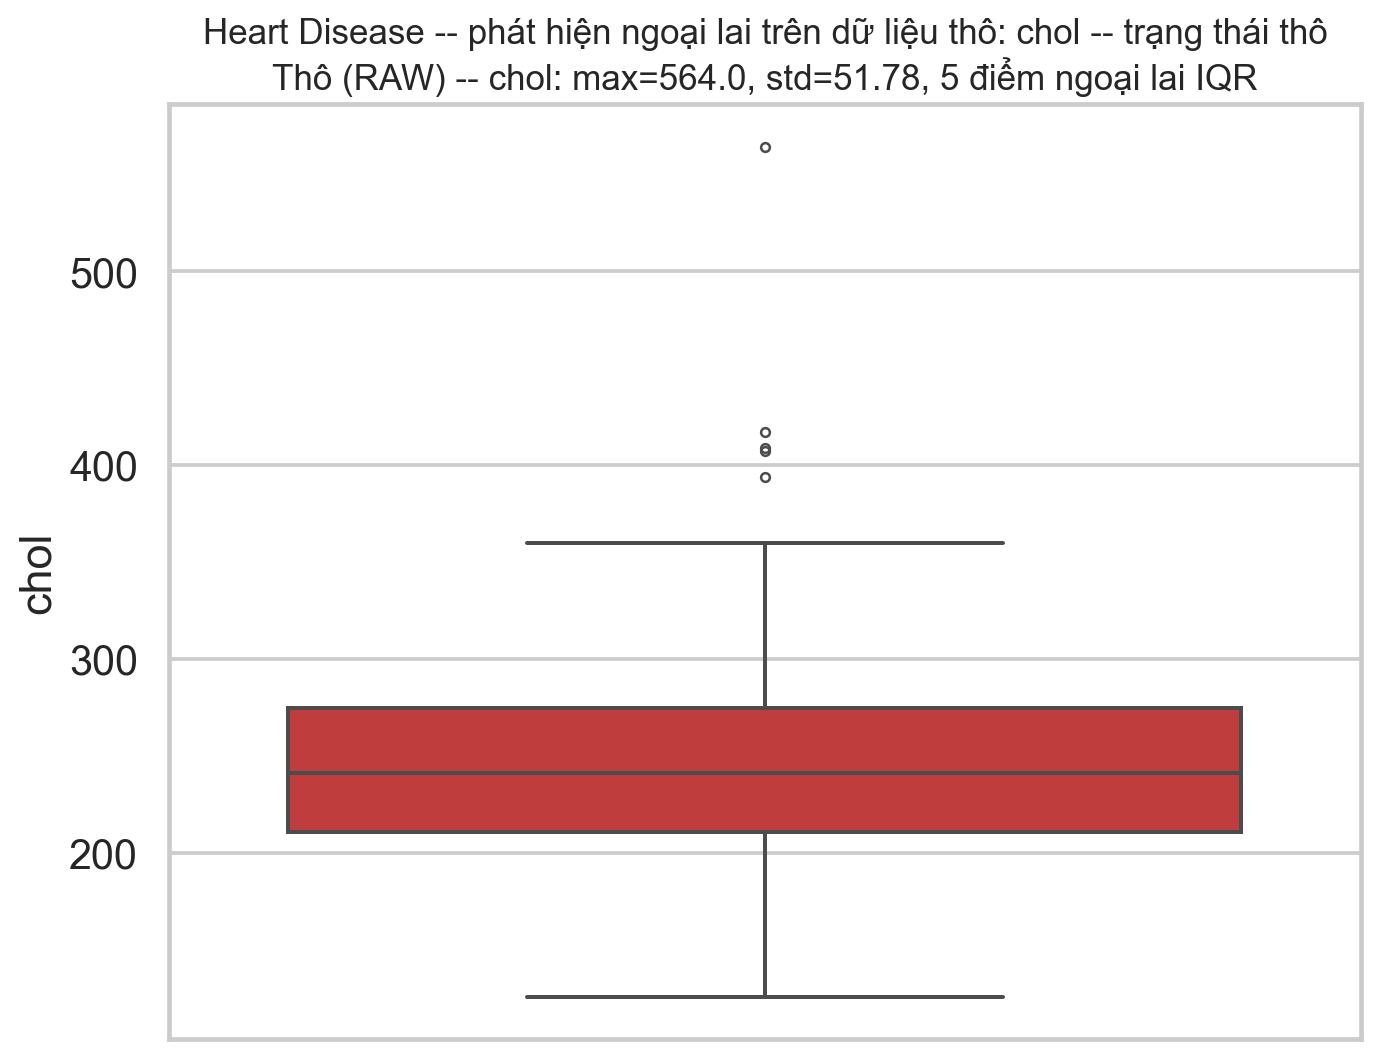
\includegraphics[width=0.72\textwidth]{images/ch3/heart_disease_chol_boxplot_raw.png}
\captionsetup{justification=raggedright,singlelinecheck=false}
\caption[Boxplot \texttt{chol} thô Heart Disease]{Boxplot \texttt{chol} Heart Disease ở \textbf{trạng thái thô}: nhiều điểm ngoại lai ở đuôi phải, giá trị lớn nhất đạt 564 mg/dL (ngưỡng trên hộp $\approx 371$).\\
\footnotesize Python source: \texttt{scripts/generate\_raw\_vs\_cleaned\_boxplots.py}.}
\label{fig:ch4_heart_raw_boxplot}
\end{figure}

\textit{Phát hiện ngoại lai trên dữ liệu thô.} Hình~\ref{fig:ch4_heart_raw_boxplot} cho thấy một số biến định lượng lâm sàng có điểm quan sát nằm ngoài râu hộp theo quy tắc IQR. Nổi bật nhất là \texttt{chol}, với giá trị lớn nhất \textbf{564 mg/dL}, vượt xa ngưỡng trên xấp xỉ $Q3+1.5IQR \approx 371$. Tương tự, \texttt{trestbps} đạt \textbf{200 mmHg} so với ngưỡng xấp xỉ 170, còn \texttt{oldpeak} đạt \textbf{6.2} so với ngưỡng xấp xỉ 4.0. Như vậy, ngoại lai chủ yếu tập trung ở các biến phản ánh cholesterol, huyết áp nghỉ và độ chênh ST khi gắng sức.

\textbf{Làm sạch dữ liệu.} Quy trình tiền xử lý được thực hiện theo ba nguyên tắc sau:

\begin{itemize}[leftmargin=*]
    \item \textbf{Điền khuyết:} \texttt{ca} và \texttt{thal} được điền bằng \textbf{median}. Cách chọn này phù hợp với các biến được mã hóa theo mức hoặc có phân phối lệch, vì median ít nhạy với giá trị cực trị hơn mean.
    \item \textbf{Xử lý ngoại lai:} \emph{clipping theo quy tắc IQR} trên các biến định lượng \texttt{age}, \texttt{trestbps}, \texttt{chol}, \texttt{thalach}, \texttt{oldpeak}, \texttt{ca} -- mọi giá trị ngoài $[Q1-1.5IQR,\; Q3+1.5IQR]$ được kéo về biên hộp (ví dụ \texttt{chol}=564 $\to$ 371, \texttt{trestbps}=200 $\to$ 170).
    \item \textbf{Chuẩn hóa:} \emph{chưa áp dụng} ở giai đoạn thống kê mô tả để giữ nguyên đơn vị lâm sàng gốc; Min--Max Scaling hoặc Z-score chỉ được dùng ở chương học máy khi thuật toán yêu cầu thang đo đồng nhất.
\end{itemize}

\begin{figure}[H]
\centering
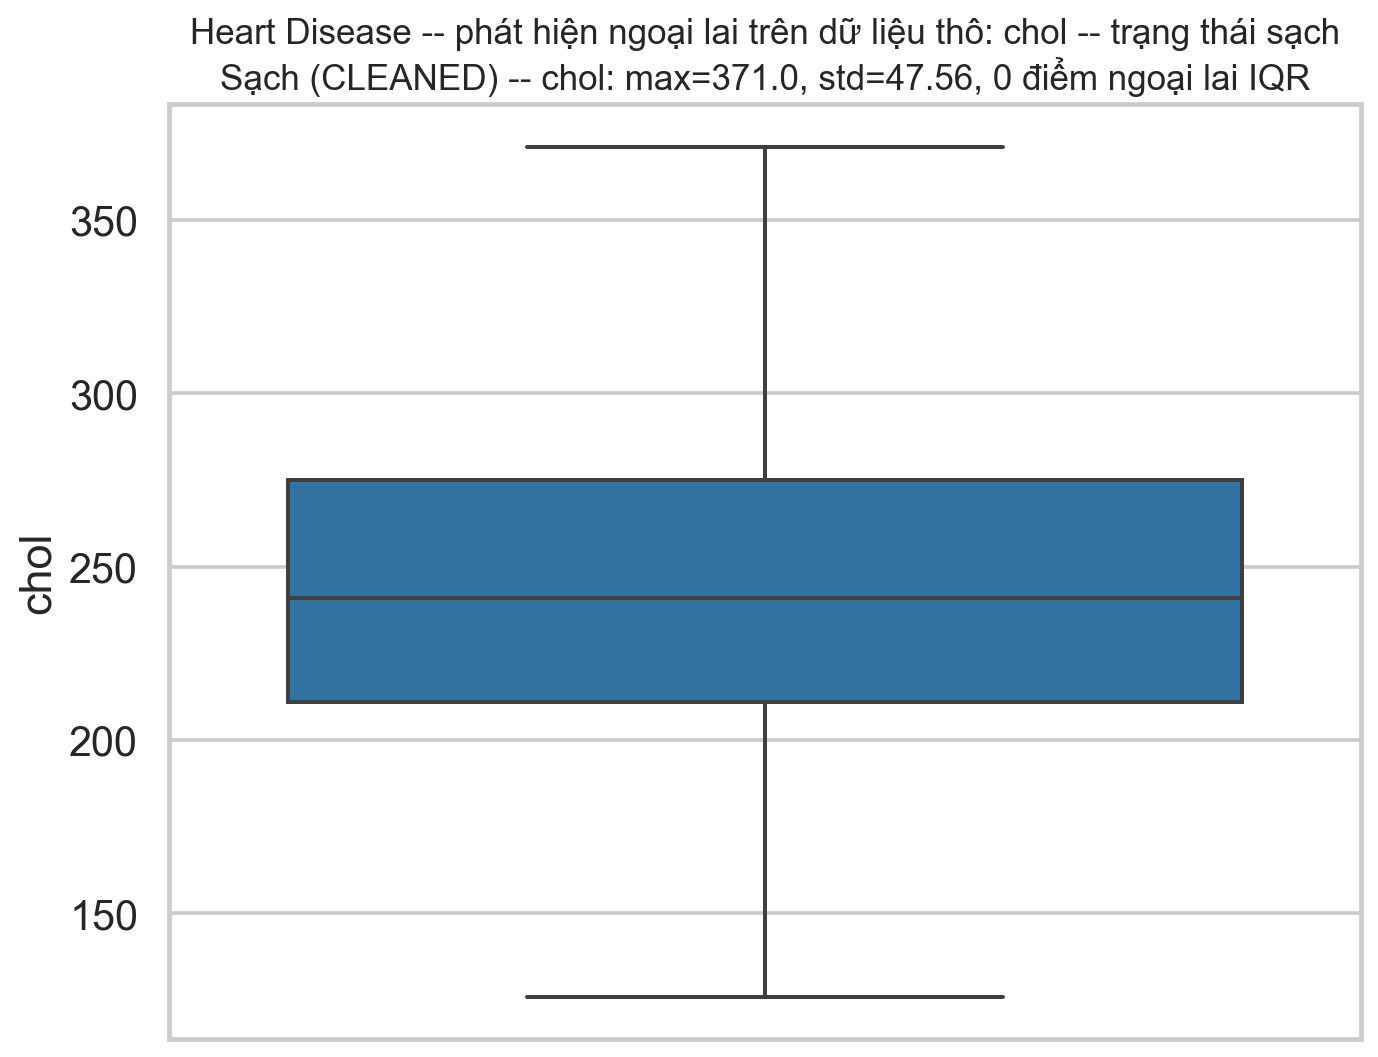
\includegraphics[width=0.72\textwidth]{images/ch3/heart_disease_chol_boxplot_cleaned.png}
\captionsetup{justification=raggedright,singlelinecheck=false}
\caption[Boxplot \texttt{chol} sạch Heart Disease]{Boxplot \texttt{chol} Heart Disease ở \textbf{trạng thái sạch}: sau clipping IQR, các điểm ngoại lai đuôi phải được nén về ngưỡng trên hộp, max giảm từ 564 xuống $\approx 371$.\\
\footnotesize Python source: \texttt{scripts/generate\_raw\_vs\_cleaned\_boxplots.py}.}
\label{fig:ch4_heart_cleaned_boxplot}
\end{figure}

\textbf{Bước 1. Phân loại bản chất biến.} Trước khi lựa chọn thống kê và biểu đồ, các biến được phân loại theo bản chất đo lường. Cách phân loại này giúp tránh áp dụng sai chỉ số, chẳng hạn không dùng mean/median để diễn giải biến định danh như \texttt{cp}.

\vspace{1\baselineskip}

\begin{table}[H]
\centering
\caption{Phân loại biến tiêu biểu trong Heart Disease}
\label{tab:ch4_heart_variable_types}
\small
\begin{tabularx}{\textwidth}{p{0.18\textwidth}p{0.27\textwidth}p{0.25\textwidth}Y}
\toprule
Biến & Bản chất & Thống kê dùng & Biểu đồ phù hợp \\
\midrule
\texttt{age} & Quantitative Discrete & Mean, median, SD, IQR & Histogram, boxplot \\
\texttt{cp} & Qualitative (nominal) & Tần suất, tần suất tương đối, mode & Bar chart, pie chart \\
\texttt{trestbps} & Quantitative Continuous & Range, SD, IQR & Histogram, boxplot \\
\texttt{chol} & Quantitative Continuous & Dữ liệu bất thường theo IQR & Boxplot thô--sạch \\
\texttt{thalach} & Quantitative Continuous & Tương quan với tuổi/target & Scatter plot \\
\texttt{oldpeak} & Quantitative Continuous & Độ lệch phải, CV & Histogram, boxplot \\
\bottomrule
\end{tabularx}
\end{table}

\textbf{Bước 2. Bảng tần suất và thống kê mô tả.} Với biến Qualitative, báo cáo sử dụng tần suất tuyệt đối, tần suất tương đối và mode. Với biến Quantitative, báo cáo sử dụng các số đo xu hướng trung tâm và độ phân tán như mean, median, standard deviation, range và IQR.

\begin{table}[H]
\centering
\caption[Bảng tần suất biến \texttt{cp} trong Heart Disease]{Bước 2 -- Bảng tần suất biến \texttt{cp} trong Heart Disease. Source: \texttt{outputs/tables/heart\_disease\_frequency\_cp.csv}.}
\label{tab:ch4_cp_frequency}
\small
\begin{tabular}{lrr}
\toprule
Loại đau ngực \texttt{cp} & Tần suất tuyệt đối & Tần suất tương đối \\
\midrule
4.0 (không triệu chứng) & 144 & 47.52\% \\
3.0 (đau không điển hình) & 86 & 28.38\% \\
2.0 (đau điển hình) & 50 & 16.50\% \\
1.0 (đau thắt ngực điển hình) & 23 & 7.59\% \\
\bottomrule
\end{tabular}
\end{table}

Bảng \ref{tab:ch4_cp_frequency} cho thấy mode của \texttt{cp} là lớp 4.0; gần một nửa bệnh nhân thuộc nhóm đau ngực không triệu chứng. Kết quả này có ý nghĩa lâm sàng đáng chú ý: nếu chỉ dựa vào triệu chứng đau ngực điển hình, nguy cơ bệnh tim có thể bị đánh giá thấp. Do đó, \texttt{cp} cần được diễn giải đồng thời với \texttt{thalach}, \texttt{oldpeak}, \texttt{trestbps} và các biến lâm sàng khác.

\begin{table}[H]
\centering
\caption[Phân phối tần suất các biến Qualitative Heart Disease]{Phân phối tần suất (Frequency Distribution) các biến Qualitative tiêu biểu trong Heart Disease: tần suất tuyệt đối, tần suất tương đối và Mode. Source: \texttt{outputs/tables/heart\_disease\_frequency\_*.csv}.}
\label{tab:ch4_heart_qualitative_freq}
\scriptsize
\setlength{\tabcolsep}{4pt}
\begin{tabular}{llrrr}
\toprule
Biến & Lớp & Tần suất tuyệt đối & Tần suất tương đối & Mode \\
\midrule
\texttt{sex} & 1 (nam) & 206 & 67.99\% & \multirow{4}{*}{1 (nam)} \\
 & 0 (nữ) & 97 & 32.01\% & \\
\texttt{fbs} & 0 ($\leq$ 120 mg/dl) & 258 & 85.15\% & \multirow{4}{*}{0} \\
 & 1 ($>$ 120 mg/dl) & 45 & 14.85\% & \\
\texttt{restecg} & 0 (bình thường) & 151 & 49.83\% & \multirow{6}{*}{0} \\
 & 2 (LV hypertrophy) & 148 & 48.84\% & \\
 & 1 (ST-T bất thường) & 4 & 1.32\% & \\
\texttt{exang} & 0 (không) & 204 & 67.33\% & \multirow{4}{*}{0} \\
 & 1 (có) & 99 & 32.67\% & \\
\bottomrule
\end{tabular}
\end{table}

\textbf{Nhận xét.} Đối với biến Qualitative, mean và median không phản ánh ý nghĩa thống kê phù hợp; vì vậy bảng phân phối tần suất và mode là công cụ mô tả chính. Bảng \ref{tab:ch4_heart_qualitative_freq} cho thấy mẫu Heart Disease mất cân bằng giới, với 67.99\% quan sát là nam (mode = 1). Phần lớn bệnh nhân không có đường huyết lúc đói cao (\texttt{fbs} mode = 0, 85.15\%) và không bị đau thắt ngực khi gắng sức (\texttt{exang} mode = 0, 67.33\%). Đáng chú ý, \texttt{restecg} phân bố gần như song song giữa lớp 0 (49.83\%) và lớp 2 (48.84\%), trong khi lớp 1 chỉ chiếm 1.32\%; đặc điểm này cần được lưu ý khi mã hóa one-hot cho mô hình học máy.

\begin{table}[H]
\centering
\caption[Thống kê thô/sạch Heart Disease]{So sánh thống kê mô tả Heart Disease ở hai trạng thái: \textbf{thô} (chưa làm sạch) và \textbf{sạch} (sau điền median + clipping IQR). Các cột in đậm là chỉ số thay đổi nhiều nhất. Source: \texttt{outputs/tables/heart\_disease\_summary.csv}.}
\label{tab:ch4_heart_stats_raw_clean}
\footnotesize
\setlength{\tabcolsep}{4pt}
\begin{tabular}{lcrrrrrr}
\toprule
Biến & Trạng thái & Mean & Median & \textbf{Std} & \textbf{Max} & \textbf{Range} & IQR \\
\midrule
\texttt{age} & thô & 54.44 & 56.00 & 9.04 & 77.00 & 48.00 & 13.00 \\
 & sạch & 54.44 & 56.00 & 9.04 & 77.00 & 48.00 & 13.00 \\
\midrule
\texttt{trestbps} & thô & 131.69 & 130.00 & \textbf{17.60} & \textbf{200.00} & \textbf{106.00} & 20.00 \\
 & sạch & 131.35 & 130.00 & \textbf{16.65} & \textbf{170.00} & \textbf{76.00} & 20.00 \\
\midrule
\texttt{chol} & thô & 246.69 & 241.00 & \textbf{51.78} & \textbf{564.00} & \textbf{438.00} & 64.00 \\
 & sạch & 245.58 & 241.00 & \textbf{47.56} & \textbf{371.00} & \textbf{245.00} & 64.00 \\
\midrule
\texttt{thalach} & thô & 149.61 & 153.00 & 22.88 & 202.00 & 131.00 & 32.50 \\
 & sạch & 149.65 & 153.00 & 22.73 & 202.00 & 117.25 & 32.50 \\
\midrule
\texttt{oldpeak} & thô & 1.04 & 0.80 & 1.16 & 6.20 & 6.20 & 1.60 \\
 & sạch & 1.02 & 0.80 & 1.11 & 4.00 & 4.00 & 1.60 \\
\bottomrule
\end{tabular}
\end{table}

\textit{Nhận xét thô/sạch.} Các biến ít chịu ảnh hưởng của ngoại lai như \texttt{age} và \texttt{thalach} gần như không thay đổi sau tiền xử lý. Ngược lại, \texttt{chol} giảm standard deviation từ 51.78 xuống 47.56, giá trị lớn nhất từ 564 xuống 371 và range từ 438 xuống 245; \texttt{trestbps} cũng giảm giá trị lớn nhất từ 200 xuống 170. Mean và median gần như ổn định, cho thấy clipping chủ yếu kiểm soát phần đuôi cực trị mà không làm thay đổi cấu trúc trung tâm của phân phối.

\textbf{Nhận xét về hình dáng phân phối.} Quan hệ giữa mean, median và mode cho phép nhận diện sơ bộ hướng lệch của phân phối. Trong Heart Disease, \texttt{age} có mean 54.44 \textless{} median 56 \textless{} mode 58, cho thấy phân phối \emph{lệch trái nhẹ}; mẫu dữ liệu tập trung nhiều ở nhóm trung niên và cao tuổi. Ngược lại, \texttt{chol} và \texttt{oldpeak} đều có mean lớn hơn median (\texttt{oldpeak}: 1.02 so với 0.80, mode = 0), phản ánh phân phối \emph{lệch phải}. Riêng \texttt{oldpeak} lệch phải rõ vì nhiều bệnh nhân có ST depression bằng 0, làm mode nằm ở biên thấp của thang đo.

\texttt{thalach} có mean 149.65 \textless{} median 153 \textless{} mode 162, cũng gợi ý phân phối lệch trái, phù hợp với hiện tượng một số bệnh nhân lớn tuổi hoặc có hạn chế gắng sức đạt nhịp tim tối đa thấp. Về độ phân tán, CV của \texttt{oldpeak} đạt 1.084, cao hơn rõ rệt so với \texttt{age}, \texttt{trestbps} và \texttt{thalach} (0.13--0.17). IQR của \texttt{chol} bằng 64 và là một trong các khoảng tứ phân vị lớn nhất trong nhóm biến lâm sàng, vì vậy boxplot là biểu đồ cần thiết để nhận diện các ca cholesterol cực trị. Nhìn chung, các biến liên tục có IQR tương đối hẹp nhưng range rộng (ví dụ \texttt{chol}: IQR 64 so với range 245), cho thấy phần lớn quan sát tập trung quanh vùng trung tâm nhưng vẫn tồn tại đuôi phân phối dài, một đặc điểm thường gặp trong dữ liệu y tế thực tế.

\textbf{Bước 3. Trực quan hóa dữ liệu.} Hệ thống biểu đồ được lựa chọn theo bản chất biến: bar chart cho biến định tính, histogram và boxplot cho biến định lượng một chiều, scatter plot cho quan hệ hai biến, biểu đồ phân bố target để kiểm tra cân bằng lớp và heatmap để khảo sát tương quan tuyến tính giữa các biến định lượng.

\begin{figure}[H]
\centering
\begin{subfigure}{0.92\textwidth}
 \centering
 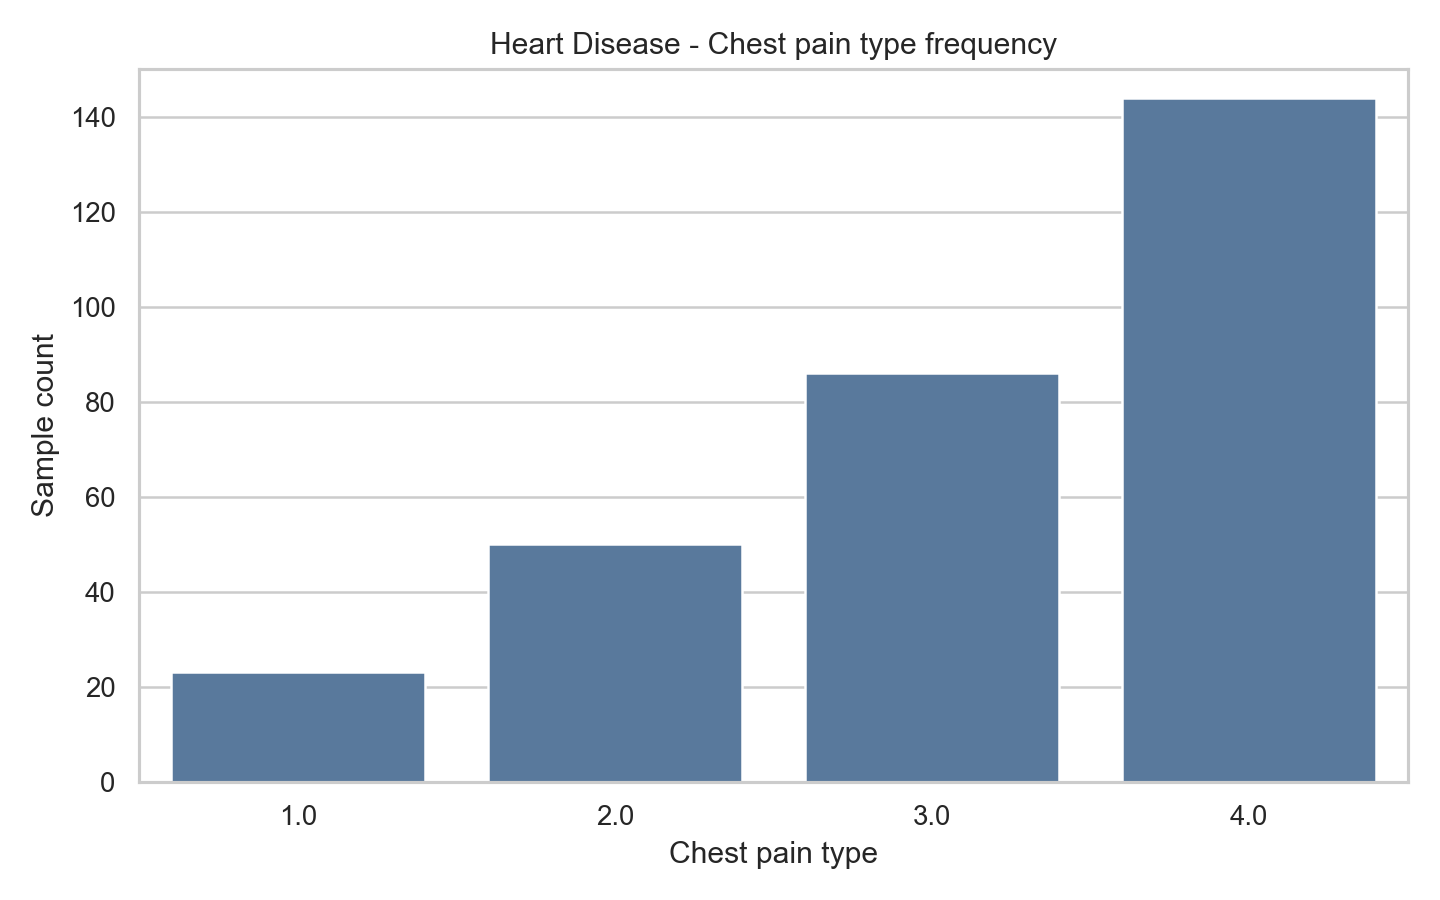
\includegraphics[width=\textwidth]{images/ch3/heart_disease_chest_pain_bar.png}
 \caption{Python -- Bar chart \texttt{cp}}
\end{subfigure}

\par\medskip

\begin{subfigure}{0.92\textwidth}
 \centering
 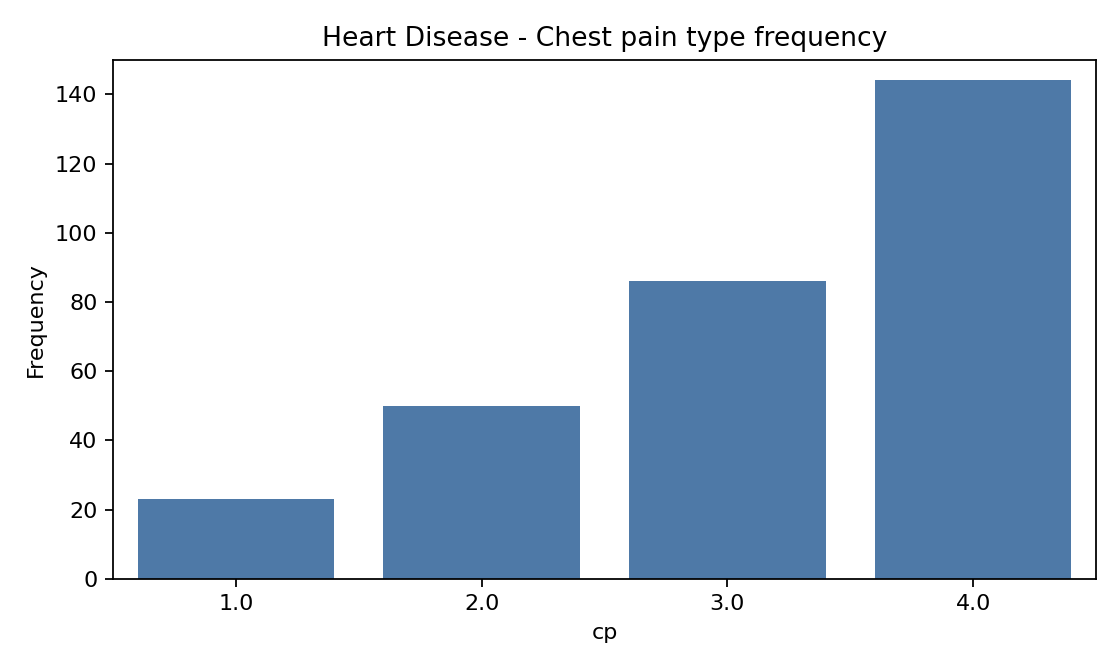
\includegraphics[width=\textwidth]{images/ch3/excel_heart_cp_bar_preview.png}
 \caption{Excel -- Column chart \texttt{cp}}
\end{subfigure}
\captionsetup{justification=raggedright,singlelinecheck=false}
\caption[Bar chart tần suất \texttt{cp}: Python và Excel]{Tần suất loại đau ngực Heart Disease vẽ bằng Python và Excel.\\
\footnotesize Python source: \texttt{src/analyze\_heart\_disease.py}.\\
Excel source/workbook: \texttt{src/create\_excel\_visualizations.py}, \texttt{excel/excel\_visualization\_comparison\_native.xlsx}, sheet \texttt{Heart Frequency}.}
\label{fig:ch4_cp_bar}
\end{figure}

\textbf{Nhận xét Hình \ref{fig:ch4_cp_bar}.} Hai phiên bản Python và Excel cho cùng một thông điệp: \texttt{cp=4} là nhóm có tần suất cao nhất, vượt rõ các nhóm còn lại. Vì \texttt{cp} là biến Qualitative nominal, biểu đồ cột là lựa chọn phù hợp hơn histogram; kết quả này cũng xác nhận mode trong Bảng \ref{tab:ch4_cp_frequency}.

\begin{figure}[H]
\centering
\begin{subfigure}{0.92\textwidth}
 \centering
 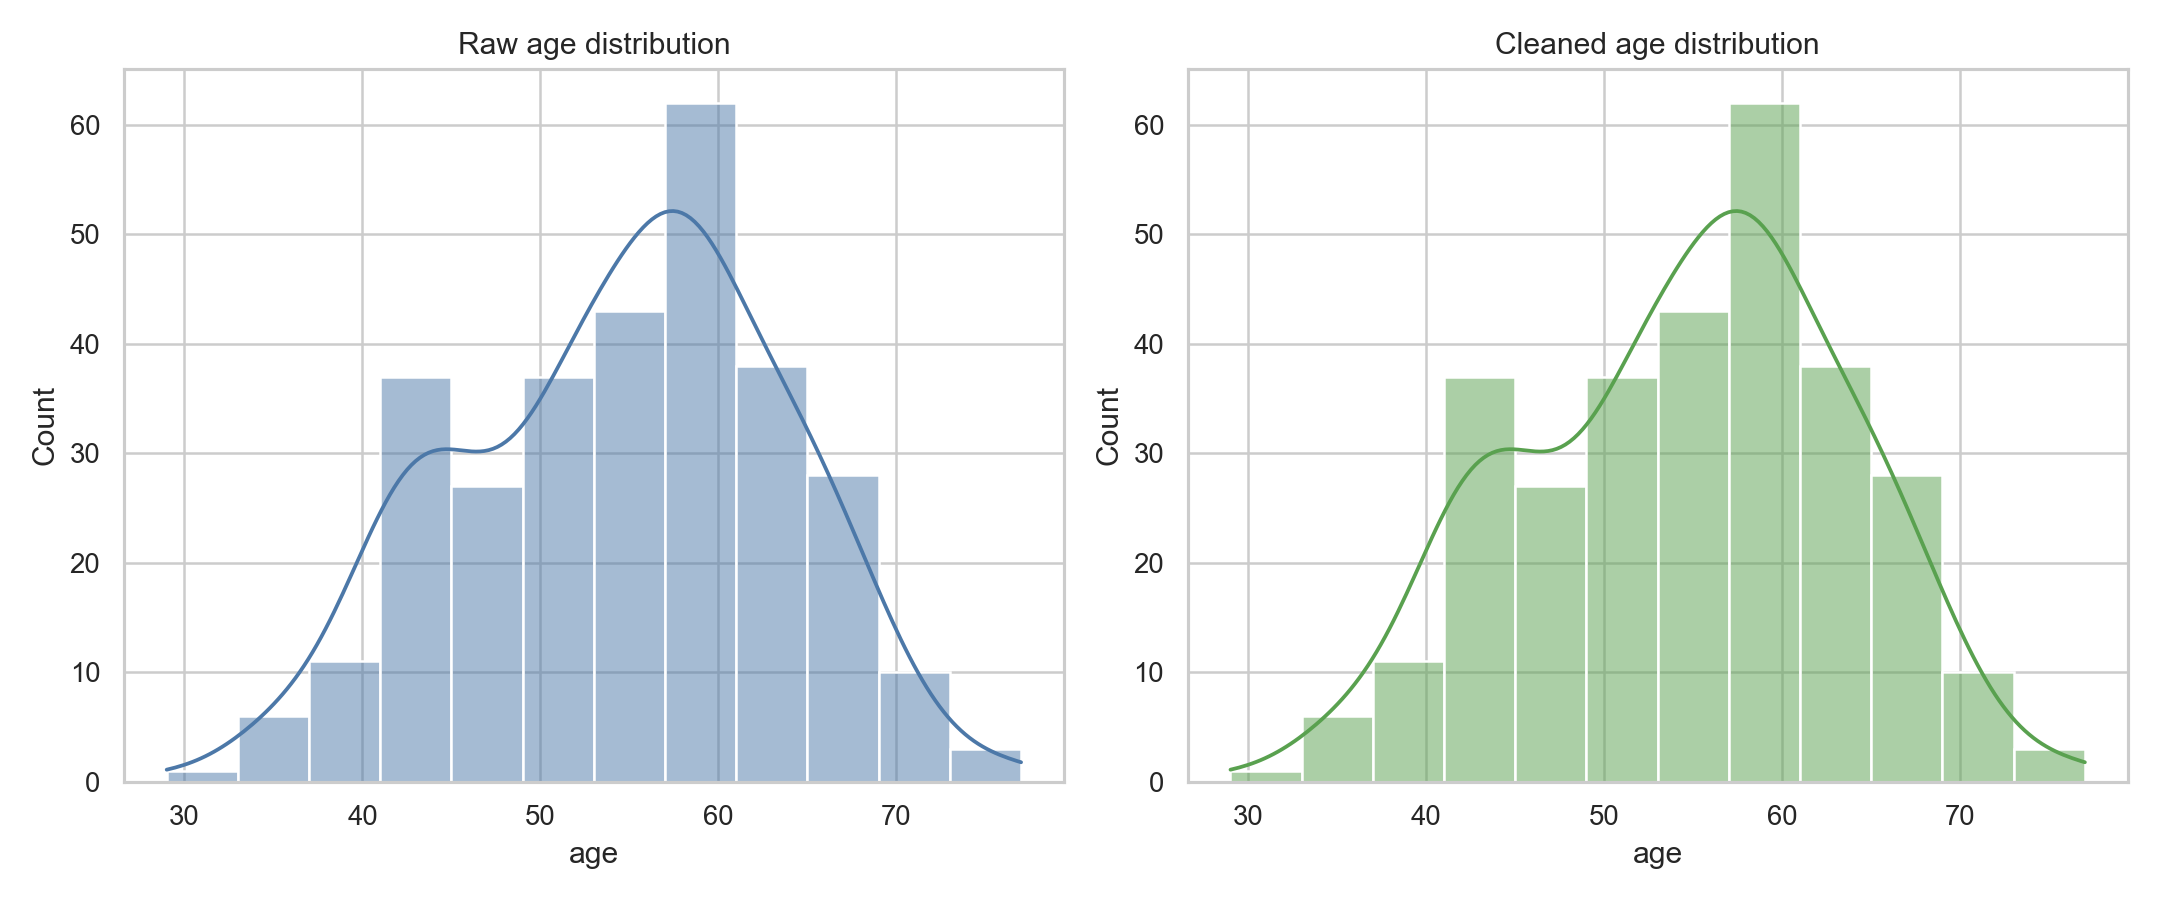
\includegraphics[width=\textwidth]{images/ch3/heart_disease_age_raw_vs_cleaned.png}
 \caption{Python -- Histogram tuổi thô/sạch}
\end{subfigure}

\par\medskip

\begin{subfigure}{0.92\textwidth}
 \centering
 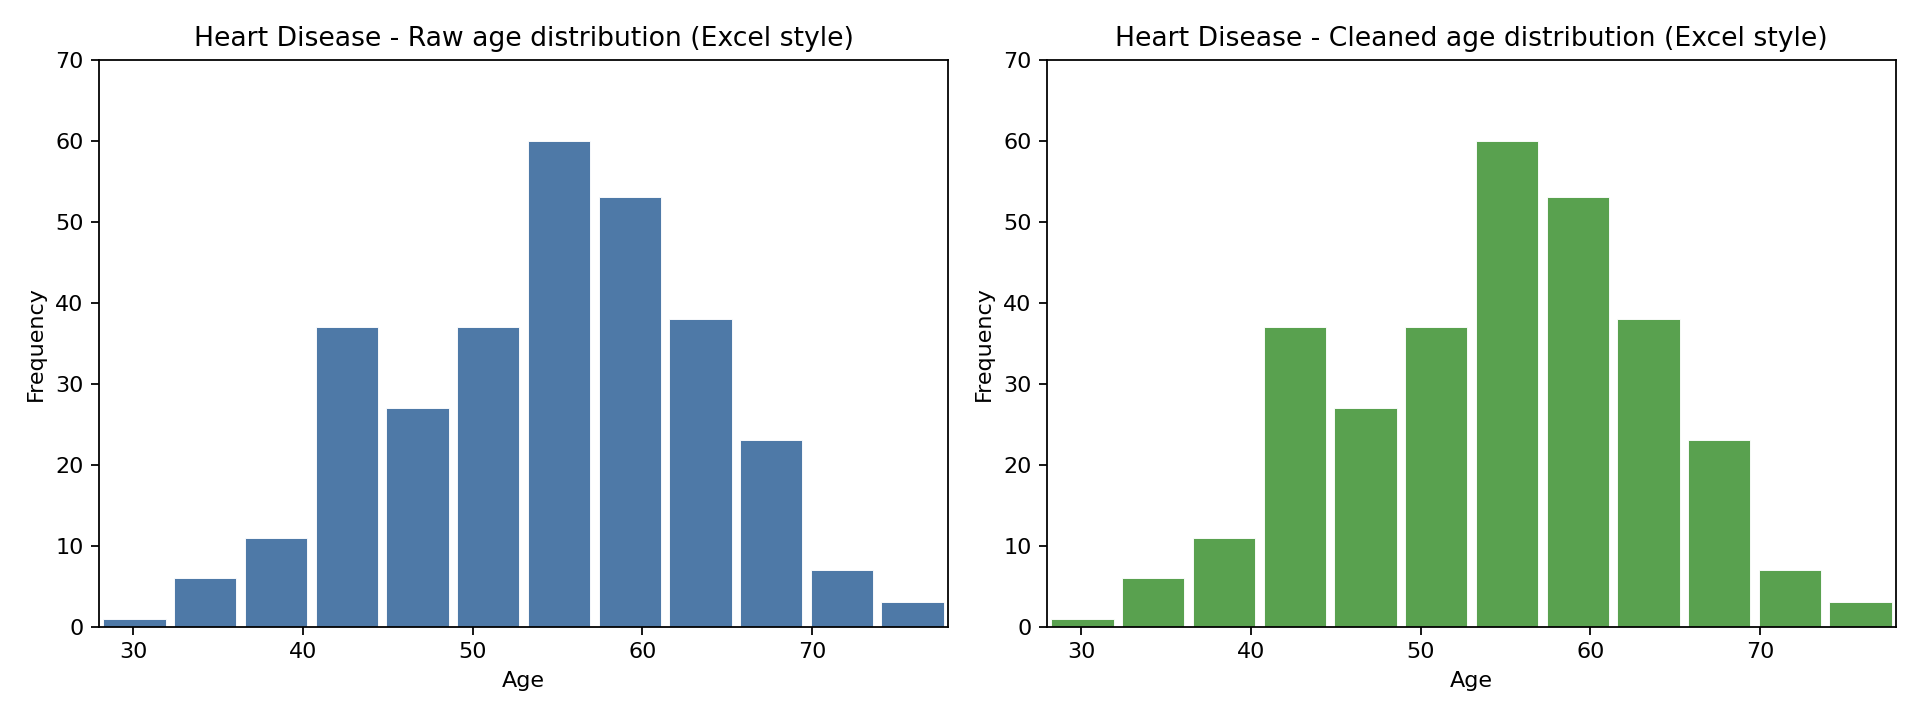
\includegraphics[width=\textwidth]{images/ch3/excel_heart_age_raw_vs_cleaned_preview.png}
 \caption{Excel -- Histogram tuổi thô/sạch}
\end{subfigure}
\captionsetup{justification=raggedright,singlelinecheck=false}
\caption[Histogram tuổi Heart Disease: Python và Excel]{Histogram tuổi thô/sạch trên Heart Disease, đối chiếu giữa Python và Excel.\\
\footnotesize Python source: \texttt{src/analyze\_heart\_disease.py}.\\
Excel source/workbook: \texttt{src/create\_excel\_visualizations.py}, \texttt{excel/excel\_visualization\_comparison\_native.xlsx}, sheet \texttt{Heart Age Hist}.}
\label{fig:ch4_heart_hist}
\end{figure}

\textbf{Nhận xét Hình \ref{fig:ch4_heart_hist}.} Histogram tuổi thô và histogram tuổi sau tiền xử lý gần như trùng nhau, cho thấy biến \texttt{age} không chịu tác động đáng kể từ bước làm sạch. Phân phối tập trung ở nhóm trung niên và cao tuổi, trong đó khoảng 50--60 tuổi xuất hiện dày hơn các nhóm còn lại; kết quả này phù hợp với bối cảnh bệnh tim thường được khảo sát nhiều ở nhóm tuổi có nguy cơ cao.

\begin{figure}[H]
\centering
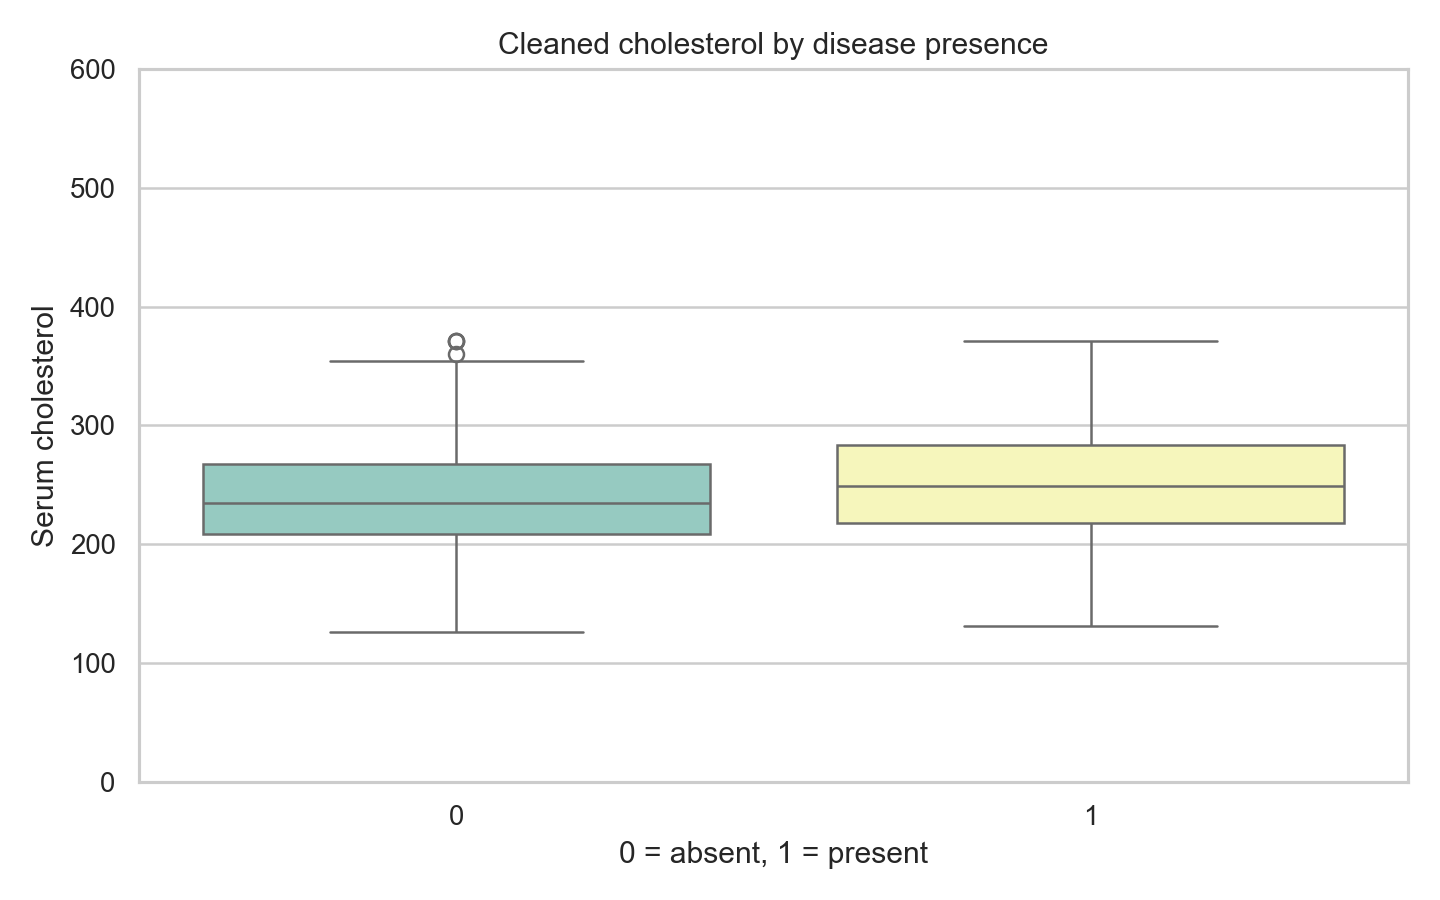
\includegraphics[width=0.92\textwidth]{images/ch3/heart_disease_cholesterol_boxplot.png}
\captionsetup{justification=raggedright,singlelinecheck=false}
\caption[Boxplot cholesterol Heart Disease]{Boxplot cholesterol trên Heart Disease.\\
\footnotesize Python source: \texttt{src/analyze\_heart\_disease.py}.}
\label{fig:ch4_heart_boxplot}
\end{figure}

\textbf{Nhận xét Hình \ref{fig:ch4_heart_boxplot}.} Boxplot cholesterol theo \texttt{target\_binary} cho thấy cả hai nhóm đều có giá trị nằm ngoài râu IQR, đặc biệt ở vùng cholesterol cao. Trung vị giữa nhóm có bệnh và không bệnh không tách biệt mạnh, vì vậy \texttt{chol} riêng lẻ chưa đủ để phân loại bệnh tim; tuy nhiên, độ trải rộng và các giá trị cực trị vẫn là thông tin lâm sàng cần được kiểm soát trong tiền xử lý.

\textit{Đối chiếu thô/sạch.} Ba biểu đồ tiếp theo đặt dữ liệu thô (đỏ) cạnh dữ liệu sạch (xanh), qua đó thể hiện trực quan tác động của điền khuyết và clipping theo IQR.

\begin{figure}[H]
\centering
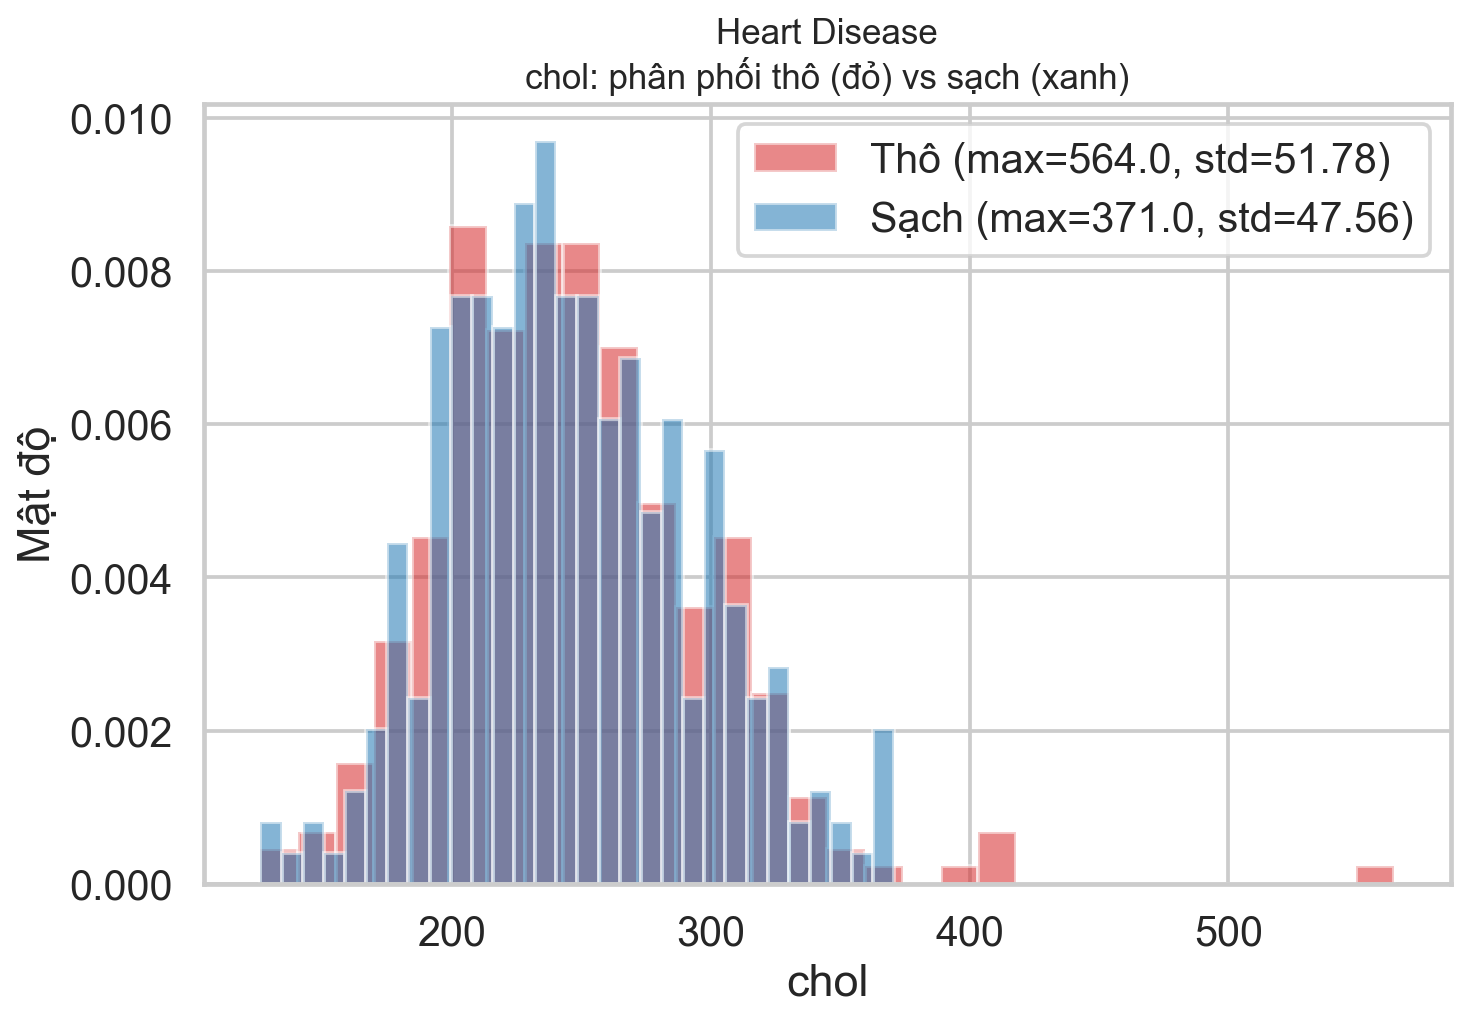
\includegraphics[width=0.82\textwidth]{images/ch3/heart_disease_chol_hist_raw_vs_cleaned.png}
\captionsetup{justification=raggedright,singlelinecheck=false}
\caption[Histogram \texttt{chol} thô/sạch Heart Disease]{Histogram \texttt{chol} Heart Disease: dữ liệu thô (đỏ, đuôi phải đến 564) chồng lên dữ liệu sạch (xanh, đuôi được nén về 371).\\
\footnotesize Python source: \texttt{scripts/generate\_raw\_vs\_cleaned\_boxplots.py}.}
\label{fig:ch4_heart_chol_hist_compare}
\end{figure}

\begin{figure}[H]
\centering
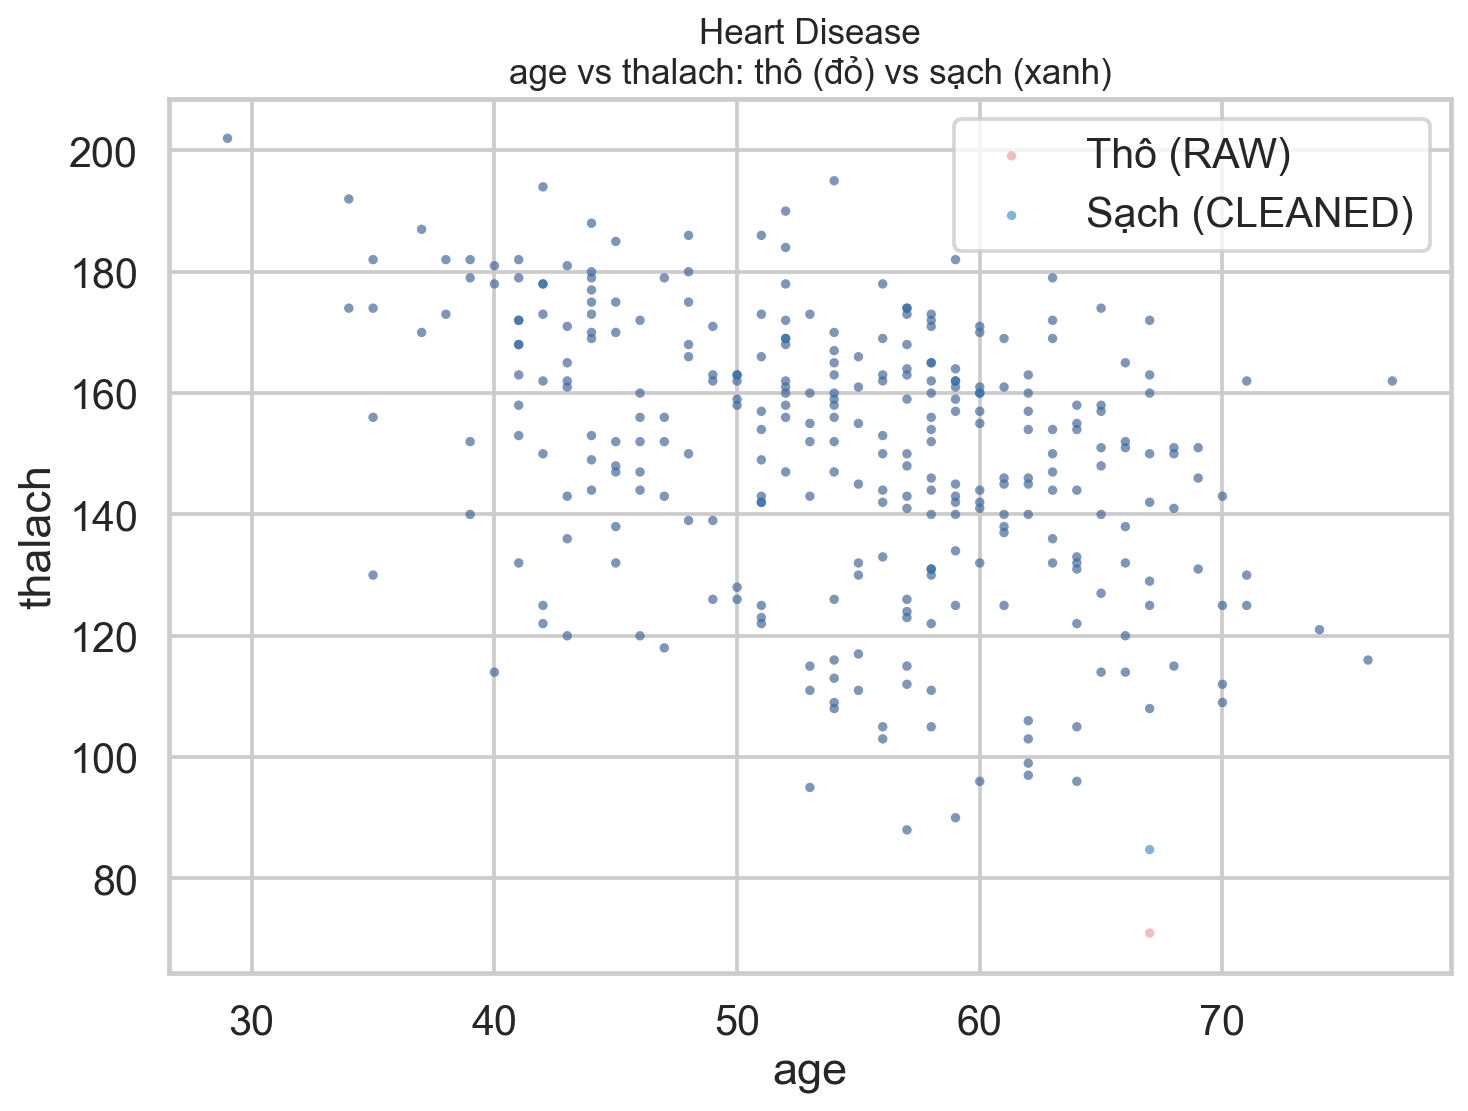
\includegraphics[width=0.82\textwidth]{images/ch3/heart_disease_age_thalach_scatter_raw_vs_cleaned.png}
\captionsetup{justification=raggedright,singlelinecheck=false}
\caption[Scatter \texttt{age}--\texttt{thalach} thô/sạch Heart Disease]{Scatter \texttt{age}--\texttt{thalach} Heart Disease: dữ liệu thô (đỏ, mờ) gần như trùng dữ liệu sạch (xanh) vì cả hai biến ít ngoại lai.\\
\footnotesize Python source: \texttt{scripts/generate\_raw\_vs\_cleaned\_boxplots.py}.}
\label{fig:ch4_heart_scatter_compare}
\end{figure}

\begin{figure}[H]
\centering
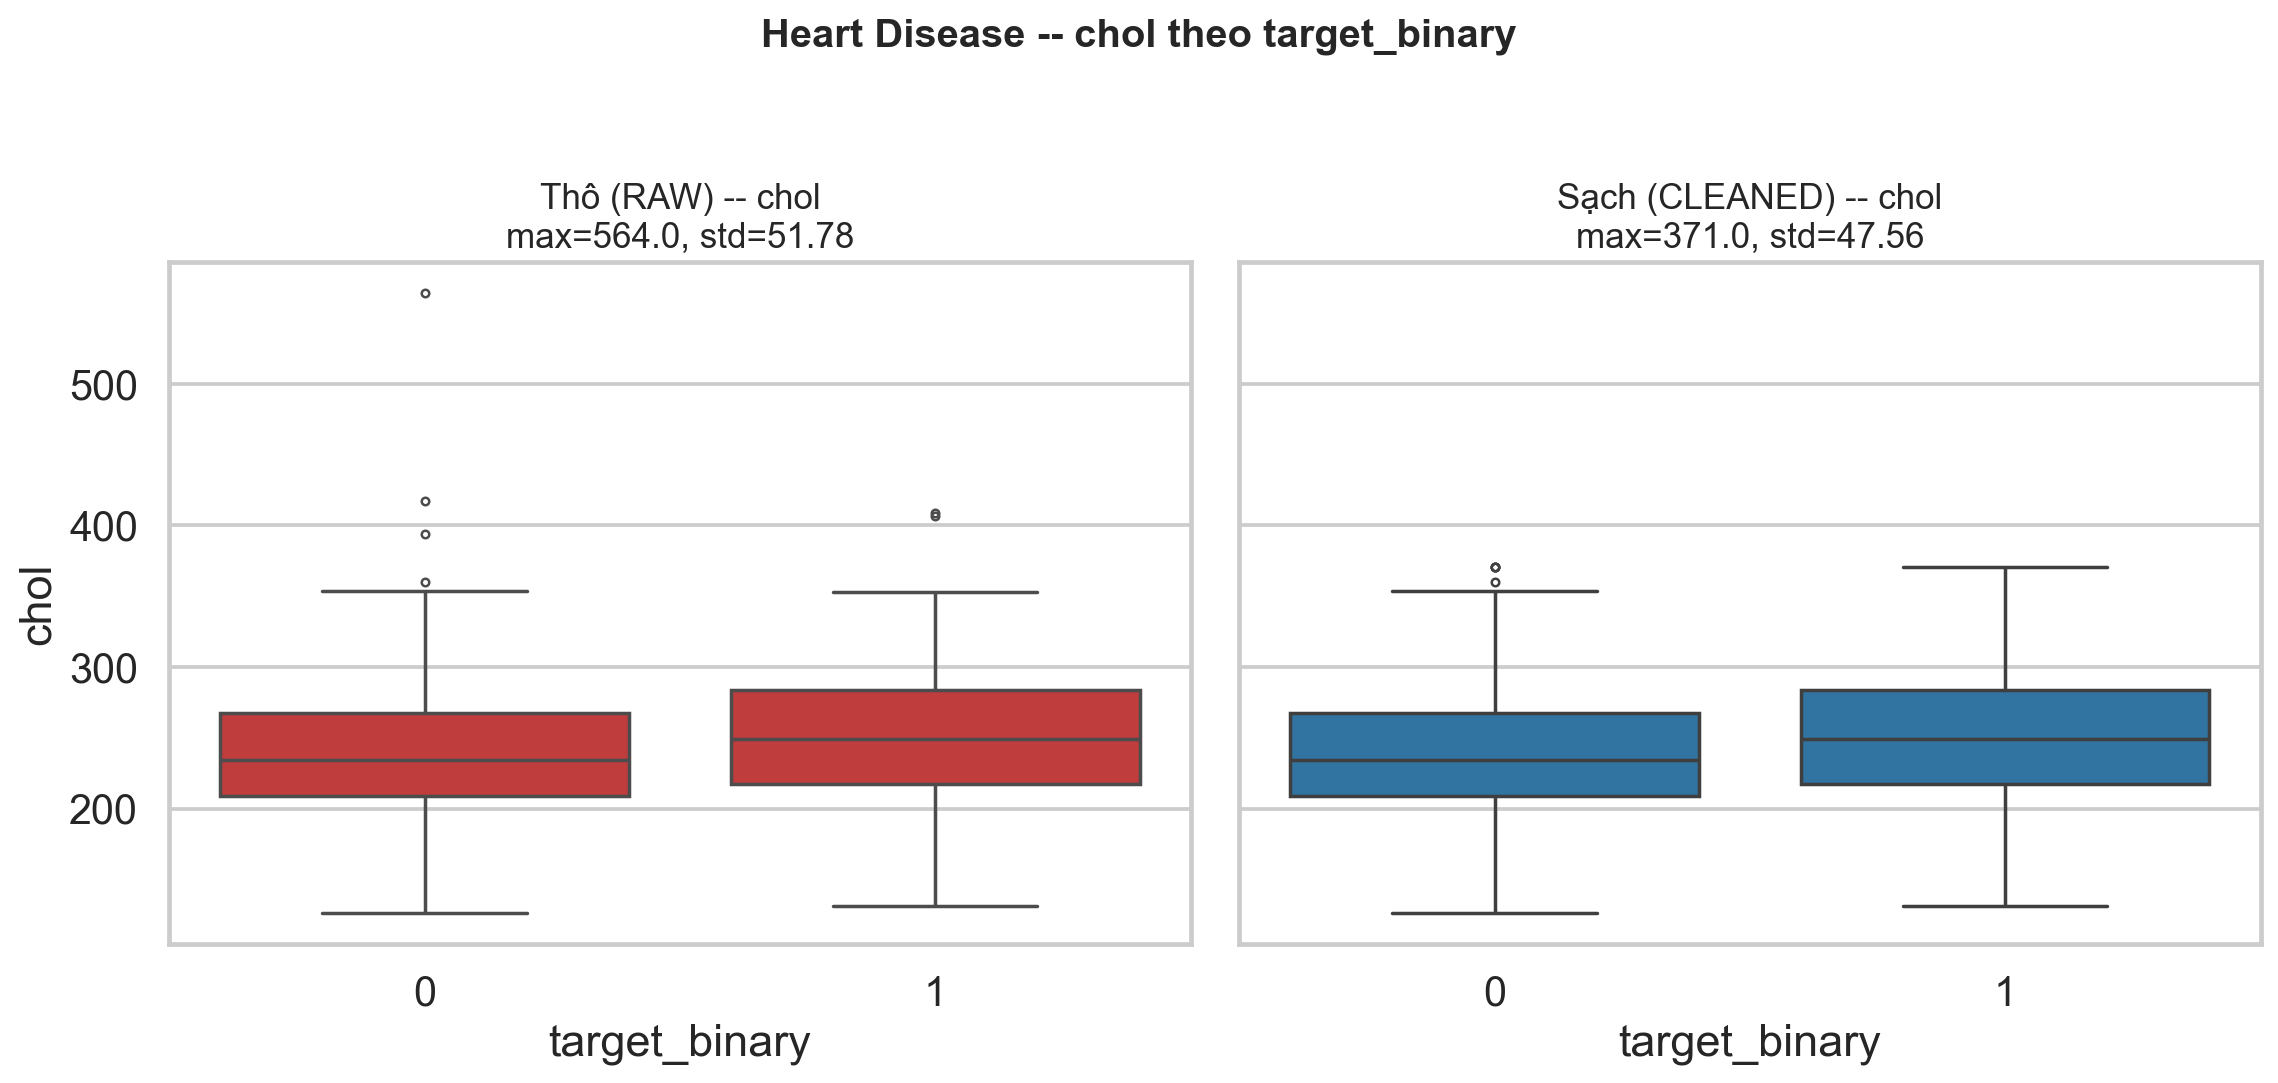
\includegraphics[width=0.95\textwidth]{images/ch3/heart_disease_chol_boxplot_by_target_raw_vs_cleaned.png}
\captionsetup{justification=raggedright,singlelinecheck=false}
\caption[Boxplot \texttt{chol} theo target thô/sạch Heart Disease]{Boxplot \texttt{chol} theo \texttt{target\_binary}: thô (trái) có nhiều điểm ngoại lai ở cả hai lớp; sạch (phải) sau clipping giảm ngoại lai nhưng vẫn giữ trung vị tách hai nhóm.\\
\footnotesize Python source: \texttt{scripts/generate\_raw\_vs\_cleaned\_boxplots.py}.}
\label{fig:ch4_heart_boxplot_by_target_compare}
\end{figure}

\textbf{Nhận xét.} Histogram \texttt{chol} (Hình~\ref{fig:ch4_heart_chol_hist_compare}) cho thấy đuôi phải của dữ liệu thô kéo dài tới 564, trong khi dữ liệu sạch dừng ở 371. Phần chồng lấn lớn giữa hai phân phối xác nhận rằng clipping chủ yếu nén vùng đuôi, không làm thay đổi phần lõi của dữ liệu. Scatter \texttt{age}--\texttt{thalach} (Hình~\ref{fig:ch4_heart_scatter_compare}) gần như trùng nhau vì hai biến này ít chịu ảnh hưởng của ngoại lai. Boxplot theo target (Hình~\ref{fig:ch4_heart_boxplot_by_target_compare}) cho thấy sau clipping, số điểm ngoài râu giảm rõ nhưng trung vị giữa hai lớp bệnh/không bệnh vẫn được duy trì, nghĩa là tín hiệu phân loại cơ bản không bị triệt tiêu.

\begin{figure}[H]
\centering
\begin{subfigure}{0.92\textwidth}
 \centering
 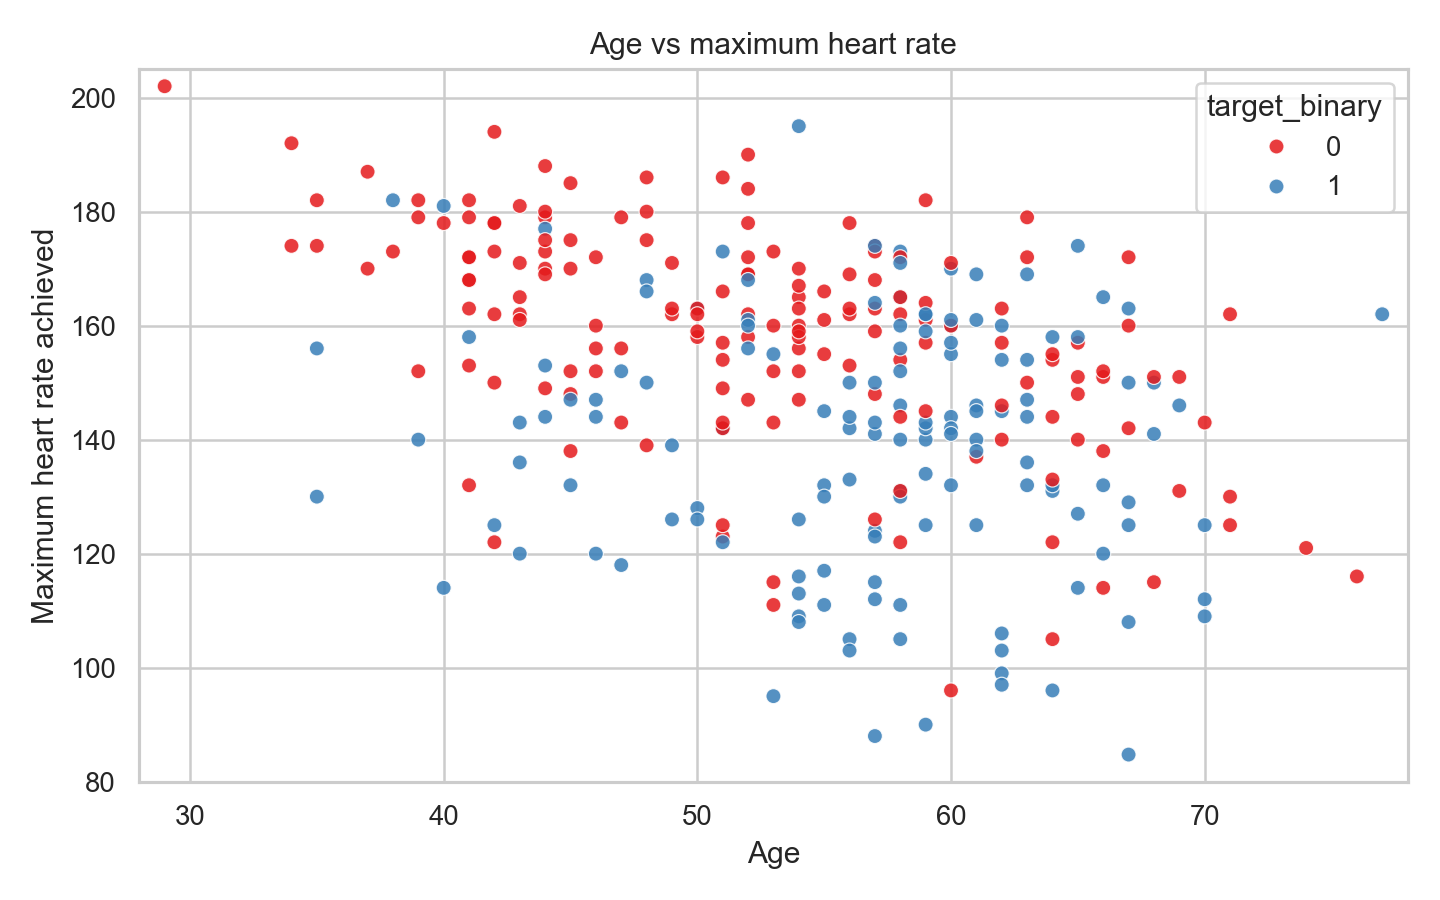
\includegraphics[width=\textwidth]{images/ch3/heart_disease_age_thalach_scatter.png}
 \caption{Python -- \texttt{age} và \texttt{thalach}}
\end{subfigure}

\par\medskip

\begin{subfigure}{0.92\textwidth}
 \centering
 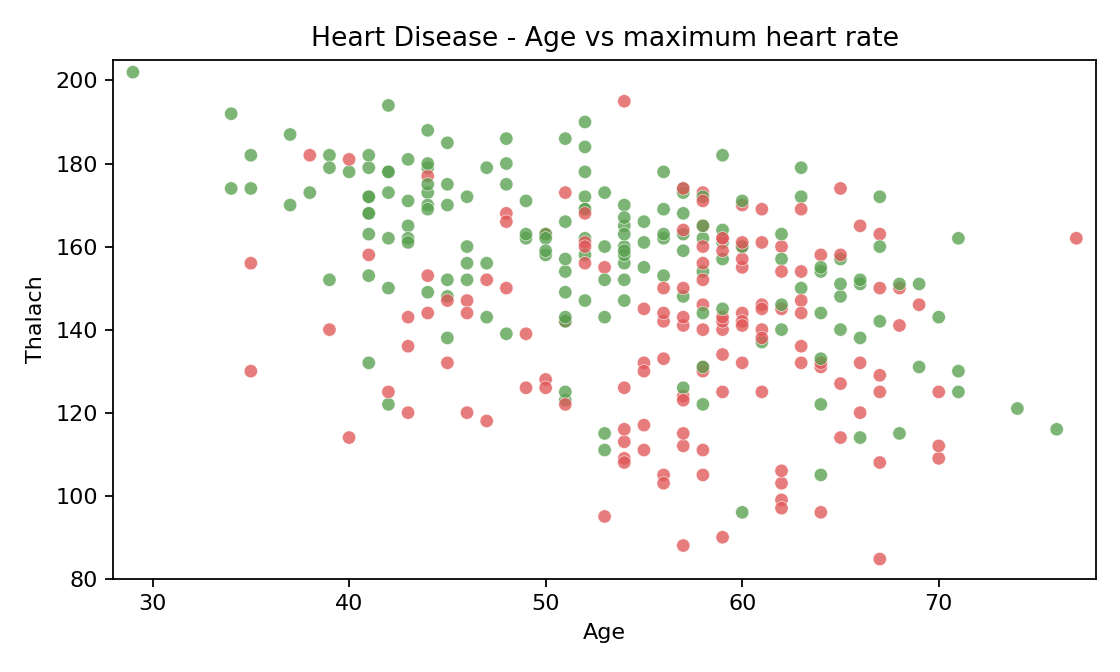
\includegraphics[width=\textwidth]{images/ch3/excel_heart_age_thalach_scatter_preview.png}
 \caption{Excel -- \texttt{age} và \texttt{thalach}}
\end{subfigure}
\captionsetup{justification=raggedright,singlelinecheck=false}
\caption[Scatter plot \texttt{age}--\texttt{thalach}: Python và Excel]{Scatter plot giữa tuổi và nhịp tim tối đa.\\
\footnotesize Python source: \texttt{src/analyze\_heart\_disease.py}.\\
Excel source/workbook: \texttt{src/create\_excel\_visualizations.py}, \texttt{excel/excel\_visualization\_comparison\_native.xlsx}, sheet \texttt{Heart Scatter}.}
\label{fig:ch4_heart_scatter}
\end{figure}

\textbf{Nhận xét Hình \ref{fig:ch4_heart_scatter}.} Scatter plot cho thấy xu hướng quan hệ âm giữa \texttt{age} và \texttt{thalach}: bệnh nhân lớn tuổi thường đạt nhịp tim tối đa thấp hơn trong kiểm tra gắng sức. Xu hướng này phù hợp về mặt sinh lý, nhưng cần được diễn giải như mối liên hệ thống kê quan sát được, không phải quan hệ nhân quả trực tiếp.

\begin{figure}[H]
\centering
\begin{subfigure}{0.92\textwidth}
 \centering
 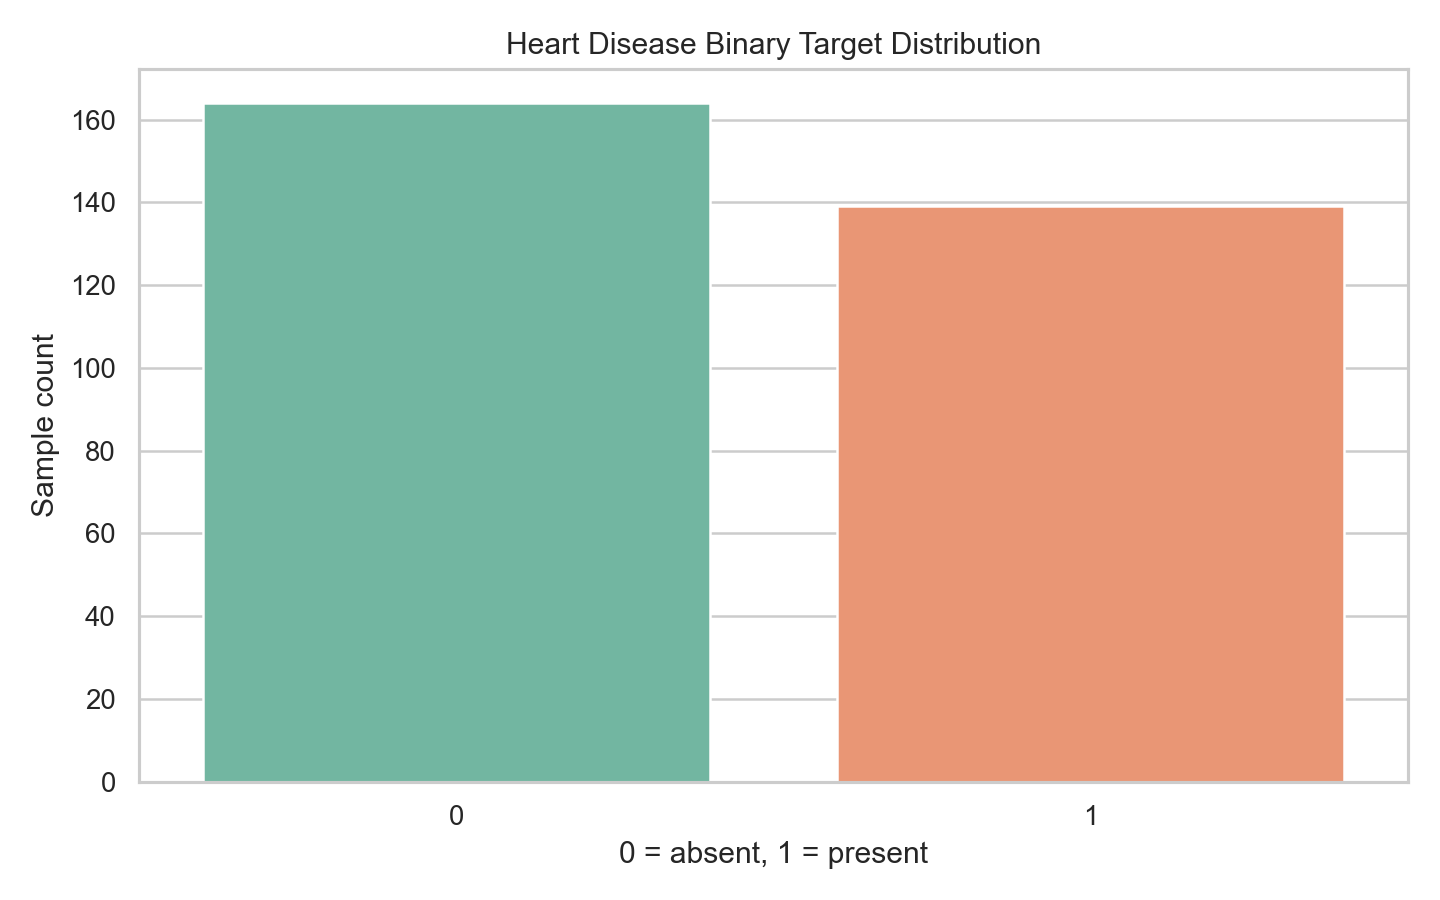
\includegraphics[width=\textwidth]{images/ch3/heart_disease_target_distribution.png}
 \caption{Python -- Phân bố target}
\end{subfigure}

\par\medskip

\begin{subfigure}{0.92\textwidth}
 \centering
 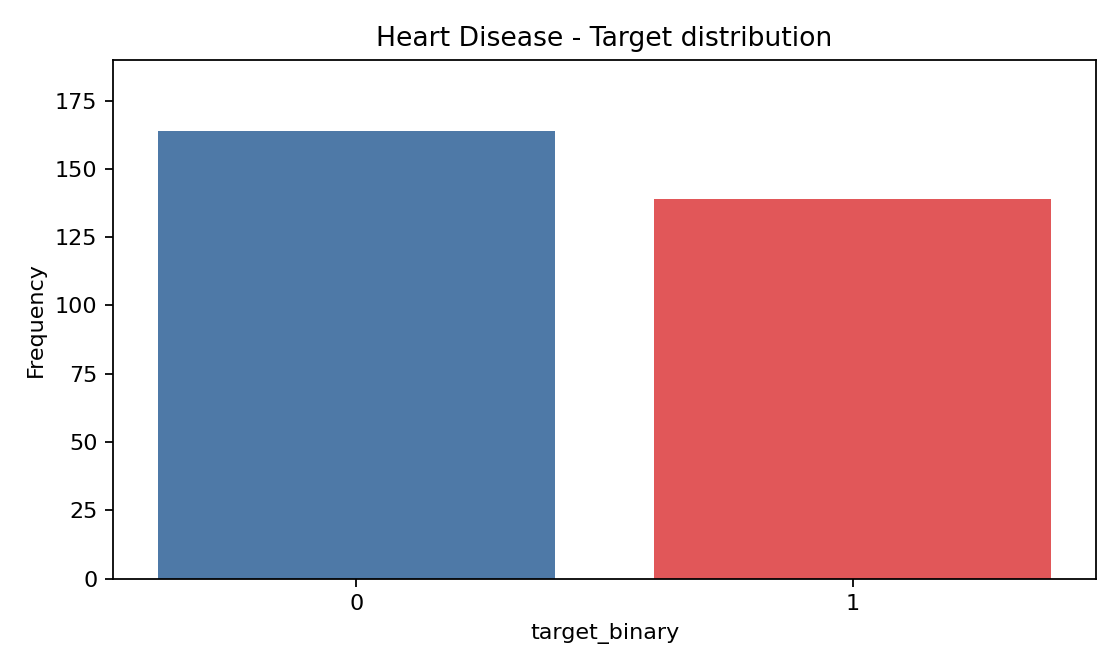
\includegraphics[width=\textwidth]{images/ch3/excel_heart_target_distribution_preview.png}
 \caption{Excel -- Phân bố target}
\end{subfigure}
\captionsetup{justification=raggedright,singlelinecheck=false}
\caption[Phân bố target Heart Disease: Python và Excel]{Phân bố target Heart Disease, đối chiếu giữa Python và Excel.\\
\footnotesize Python source: \texttt{src/analyze\_heart\_disease.py}.\\
Excel source/workbook: \texttt{src/create\_excel\_visualizations.py}, \texttt{excel/excel\_visualization\_comparison\_native.xlsx}, sheet \texttt{Heart Target}.}
\label{fig:ch4_heart_target}
\end{figure}

\textbf{Nhận xét Hình \ref{fig:ch4_heart_target}.} Phân bố target cho thấy hai lớp bệnh/không bệnh tương đối cân bằng. Vì vậy, accuracy có thể được dùng như chỉ báo ban đầu, nhưng vẫn cần đọc đồng thời precision, recall và F1 để tránh bỏ sót sai số ở từng lớp.

\begin{figure}[H]
\centering
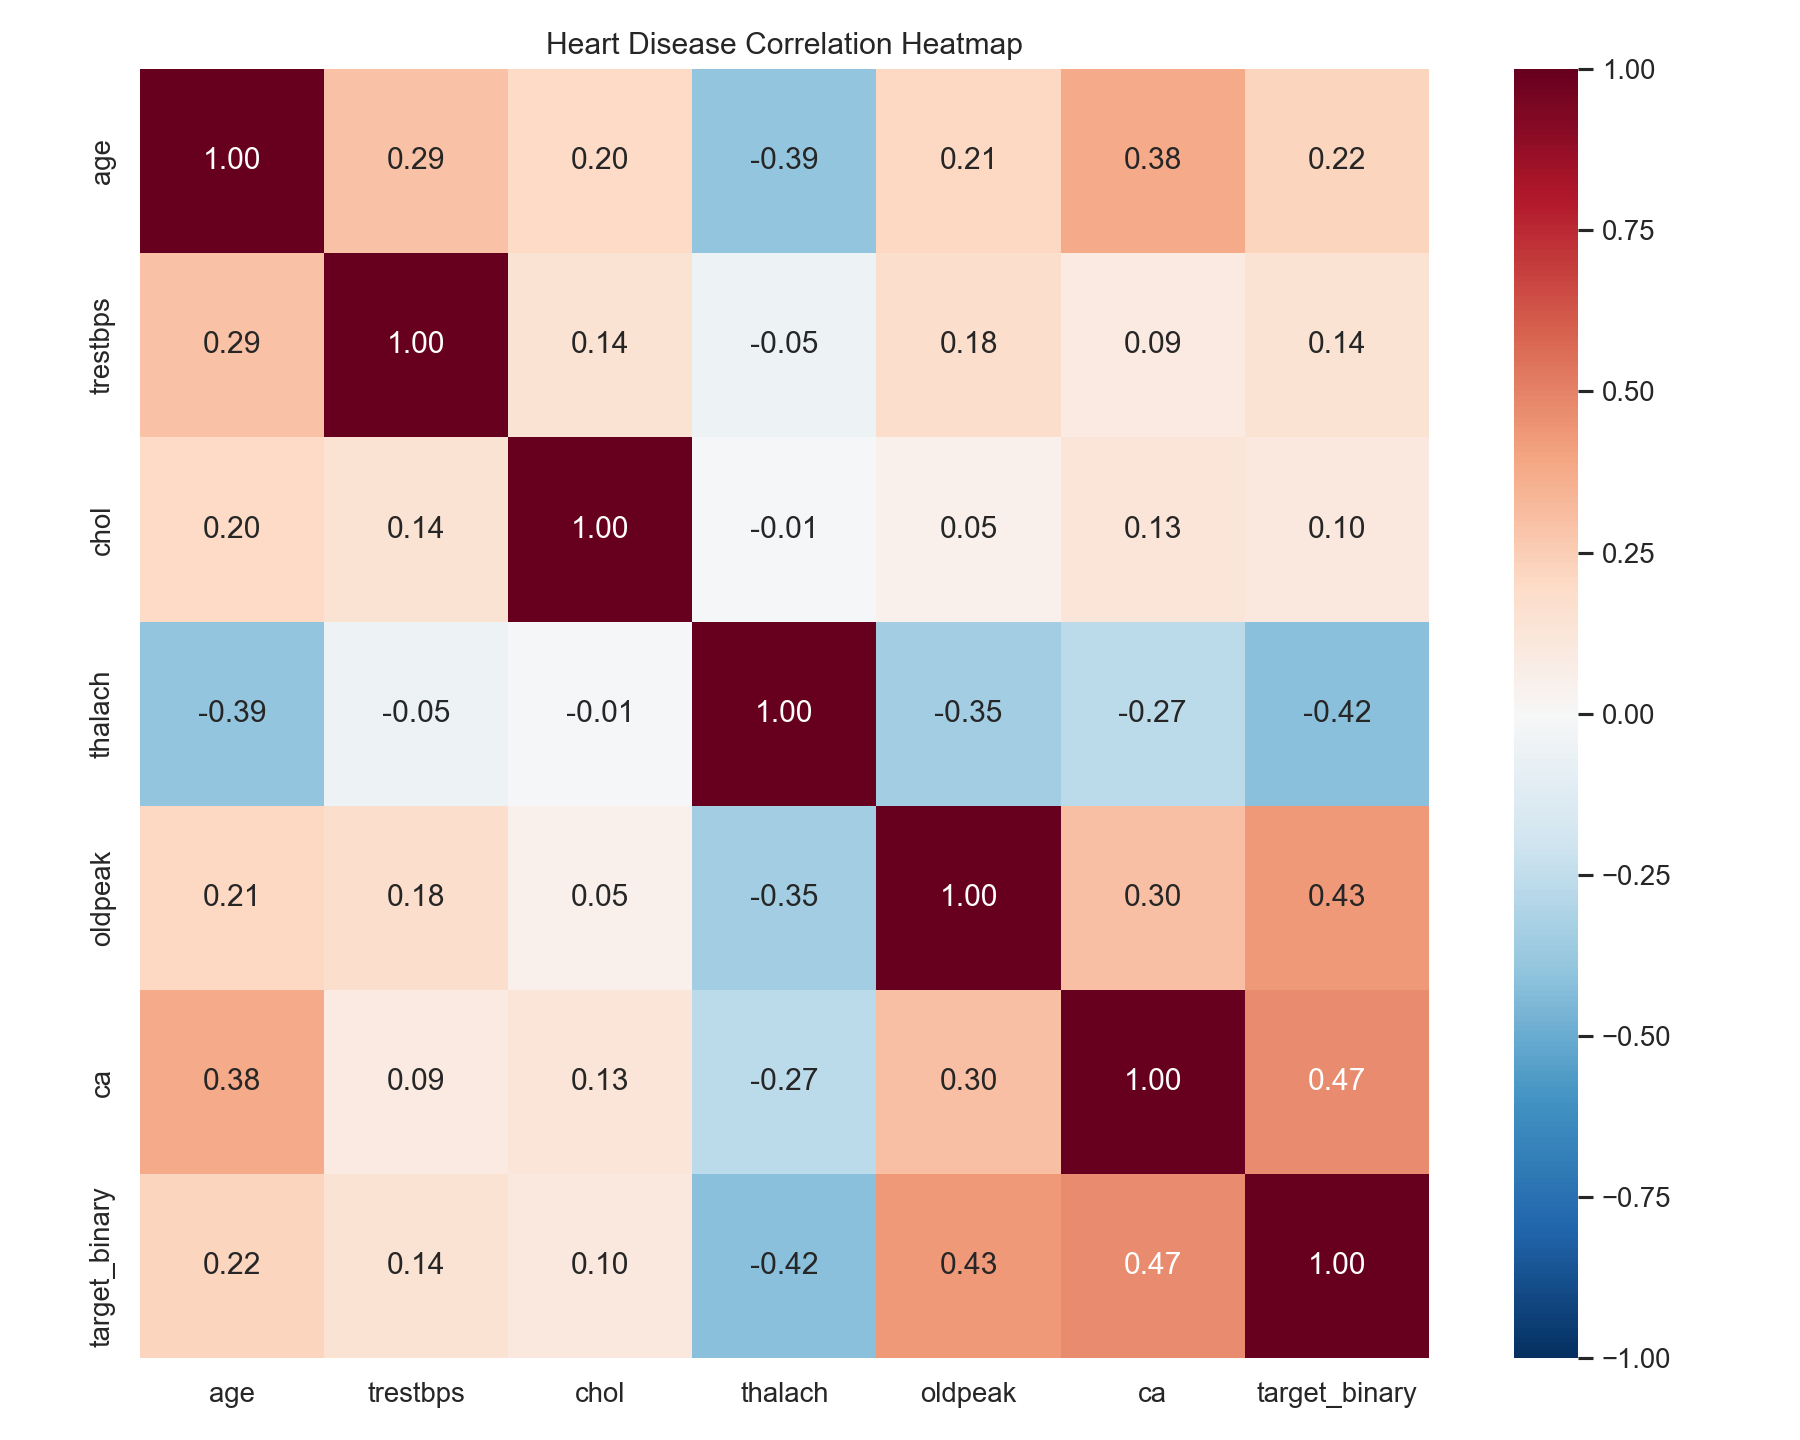
\includegraphics[width=0.86\textwidth]{images/ch3/heart_disease_correlation_heatmap.png}
\captionsetup{justification=raggedright,singlelinecheck=false}
\caption[Heatmap tương quan Heart Disease]{Heatmap tương quan các biến định lượng Heart Disease.\\
\footnotesize Python source: \texttt{src/analyze\_heart\_disease.py}.}
\label{fig:ch4_heart_corr}
\end{figure}

\textbf{Nhận xét Hình \ref{fig:ch4_heart_corr}.} Heatmap tương quan cho thấy \texttt{thalach} có tương quan âm với \texttt{target\_binary}, trong khi \texttt{oldpeak} có tương quan dương. Hai biến này phản ánh hai khía cạnh khác nhau của đáp ứng tim mạch khi gắng sức: khả năng đạt nhịp tim tối đa và mức bất thường ST. Do đó, chúng cung cấp tín hiệu bổ sung cho bài toán phân loại, dù heatmap chỉ phản ánh tương quan tuyến tính và không thay thế được đánh giá mô hình đa biến.

\textbf{Bước 4. So sánh trước--sau tiền xử lý.} Bảng~\ref{tab:ch4_heart_preprocess} đặt các chỉ số của trạng thái thô cạnh trạng thái sạch; các hình thô/sạch ở trên minh họa trực tiếp tác động của điền khuyết và clipping IQR.

\begin{table}[H]
\centering
\caption[So sánh dữ liệu thô và dữ liệu sạch Heart Disease]{Bước 4 -- So sánh dữ liệu thô và dữ liệu sạch Heart Disease (điền median cho \texttt{ca}/\texttt{thal}, clipping IQR cho biến định lượng). Source: \texttt{outputs/tables/heart\_disease\_preprocessing\_comparison.csv}.}
\label{tab:ch4_heart_preprocess}
\small
\begin{tabular}{lrrrrrr}
\toprule
Biến & Max thô & Max sạch & Std thô & Std sạch & Range thô & Range sạch \\
\midrule
\texttt{age} & 77.00 & 77.00 & 9.04 & 9.04 & 48.00 & 48.00 \\
\texttt{trestbps} & 200.00 & 170.00 & 17.60 & 16.65 & 106.00 & 76.00 \\
\texttt{chol} & 564.00 & 371.00 & 51.78 & 47.56 & 438.00 & 245.00 \\
\texttt{thalach} & 202.00 & 202.00 & 22.88 & 22.73 & 131.00 & 117.25 \\
\texttt{oldpeak} & 6.20 & 4.00 & 1.16 & 1.11 & 6.20 & 4.00 \\
\bottomrule
\end{tabular}
\end{table}

Bảng \ref{tab:ch4_heart_preprocess} cho thấy hiệu quả của xử lý ngoại lai theo IQR: \texttt{chol} giảm giá trị lớn nhất từ 564 xuống 371 và range giảm gần một nửa; \texttt{trestbps} cũng giảm giá trị lớn nhất từ 200 xuống 170. Các điểm nằm ngoài râu boxplot ở Hình \ref{fig:ch4_heart_boxplot} là nhóm quan sát cần được đánh dấu trước khi clipping. Sau xử lý, độ lệch chuẩn của \texttt{chol} giảm từ 51.78 xuống 47.56 và \texttt{trestbps} giảm từ 17.60 xuống 16.65; trong khi đó, các chỉ số trung tâm không thay đổi đáng kể. Điều này cho thấy tiền xử lý làm giảm ảnh hưởng của giá trị cực trị nhưng vẫn bảo toàn cấu trúc chính của dữ liệu.

\textbf{Kết luận cho Heart Disease.} Có ba kết quả chính rút ra từ phân tích trước--sau tiền xử lý. Thứ nhất, toàn bộ ô khuyết được xử lý sau khi điền median cho \texttt{ca} và \texttt{thal}. Thứ hai, độ phân tán của các biến có ngoại lai giảm có kiểm soát; riêng \texttt{chol} giảm standard deviation 8.1\% (51.78$\to$47.56) và range giảm 44\% (438$\to$245). Thứ ba, các biến vốn ổn định như \texttt{age} gần như không thay đổi, thể hiện qua histogram thô/sạch gần trùng nhau. Như vậy, quy trình tiền xử lý làm giảm ảnh hưởng của giá trị cực trị và ô khuyết, đồng thời vẫn giữ được xu hướng trung tâm và tín hiệu phân biệt chính của bộ dữ liệu.

\subsubsection{CDC Diabetes Health Indicators}

CDC Diabetes có 253\,680 mẫu và 21 biến giải thích, là bộ dữ liệu lớn nhất của nhóm A.

\textbf{Trạng thái dữ liệu thô (chưa làm sạch).} Ở trạng thái thô, CDC Diabetes \emph{không có ô khuyết thiếu} (0/253\,680 dòng, theo \texttt{outputs/tables/cdc\_diabetes\_missing\_values.csv}); do đó bước điền khuyết không cần thiết.

\begin{figure}[H]
\centering
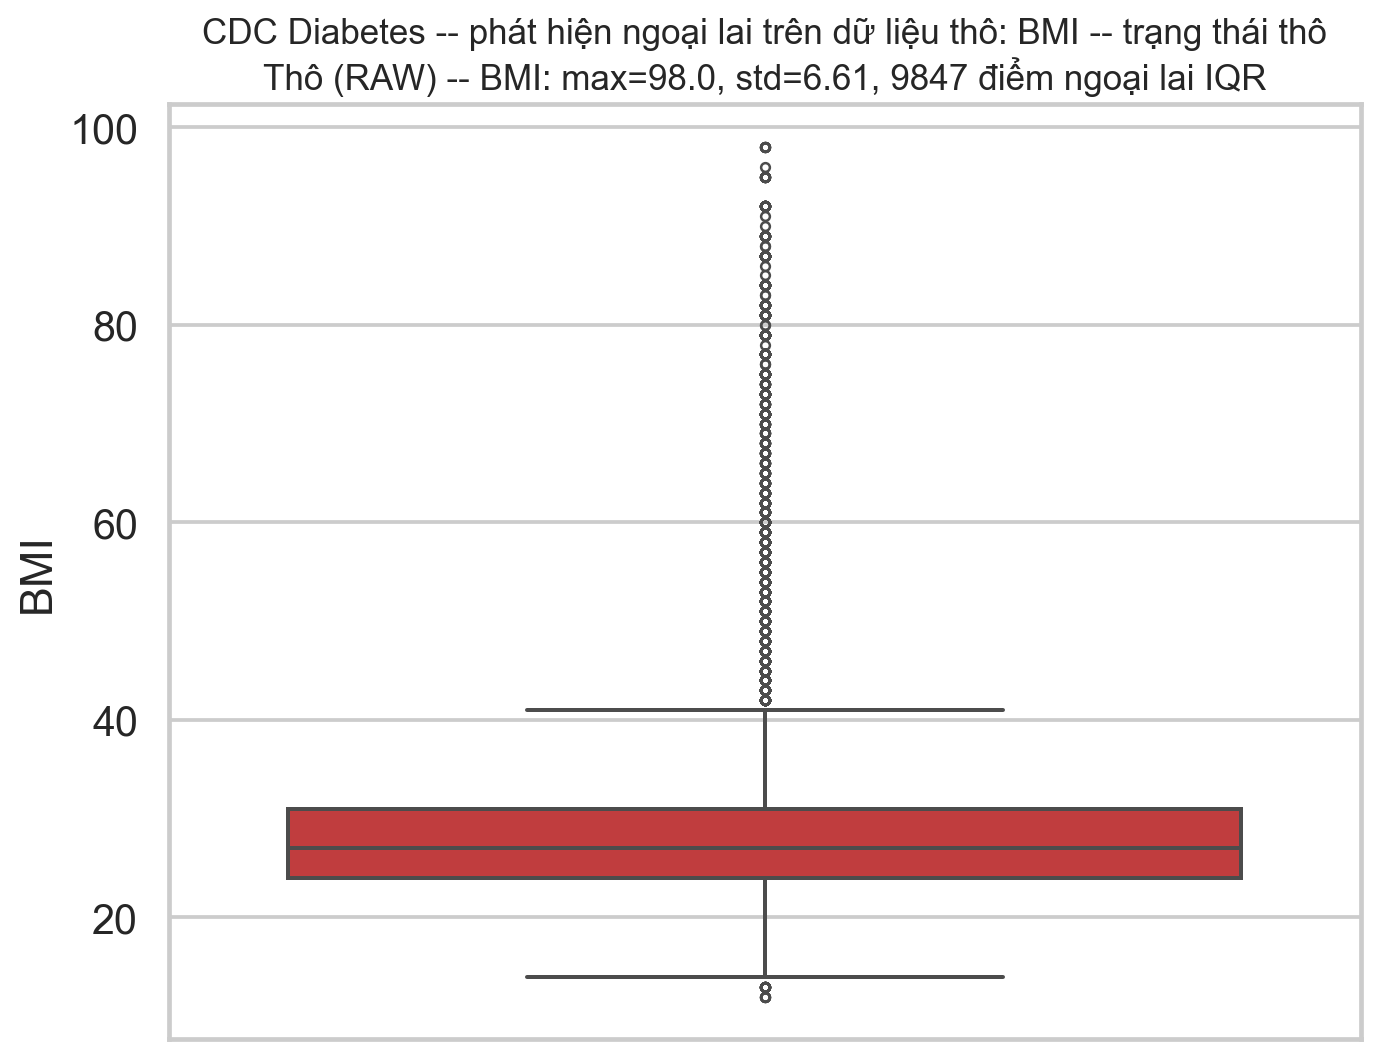
\includegraphics[width=0.72\textwidth]{images/ch3/cdc_diabetes_BMI_boxplot_raw.png}
\captionsetup{justification=raggedright,singlelinecheck=false}
\caption[Boxplot \texttt{BMI} thô CDC Diabetes]{Boxplot \texttt{BMI} CDC Diabetes ở \textbf{trạng thái thô}: hàng nghìn điểm ngoại lai ở đuôi phải tới BMI=98 (ngưỡng trên hộp $\approx 41.5$).\\
\footnotesize Python source: \texttt{scripts/generate\_raw\_vs\_cleaned\_boxplots.py}.}
\label{fig:ch4_cdc_raw_boxplot}
\end{figure}

\textit{Phát hiện ngoại lai trên dữ liệu thô (boxplot).} Dưới boxplot trạng thái thô (Hình~\ref{fig:ch4_cdc_raw_boxplot}), vấn đề chính là \emph{ngoại lai}: \texttt{BMI} có giá trị \textbf{tới 98} (béo phì bệnh lý cực đoan, so với $Q3+1.5IQR \approx 41.5$) -- hàng nghìn bệnh nhân nằm ngoài râu trên hộp ở đuôi phải; \texttt{MentHlth} và \texttt{PhysHlth} (số ngày sức khỏe tâm thần/thể chất kém trong 30 ngày) \textbf{chận 30 ngày}, gấp nhiều lần median=0, tạo các điểm rời rạc kéo dài từ giữa hộp đến giá trị cực đại; \texttt{Age} và \texttt{GenHlth} (ordinal) không có ngoại lai vì các giá trị đã nằm trong miền hợp lệ.

\textbf{Làm sạch dữ liệu.} Các bước làm sạch dữ liệu:

\begin{itemize}[leftmargin=*]
    \item \textbf{Phát hiện ngoại lai:} đã thực hiện ở trên qua boxplot -- chỉ ba biến \texttt{BMI}, \texttt{MentHlth}, \texttt{PhysHlth} có ngoại lai cực trị.
    \item \textbf{Xử lý ngoại lai:} \emph{clipping theo IQR} trên ba biến \texttt{BMI}, \texttt{MentHlth}, \texttt{PhysHlth} (ví dụ \texttt{BMI}=98 $\to$ 41.5, \texttt{MentHlth}/\texttt{PhysHlth} max 30 $\to$ 5.0/7.5).
    \item \textbf{Biến ordinal/nhị phân:} \texttt{Age}, \texttt{GenHlth} giữ nguyên mã lớp vì không có ngoại lai trong miền hợp lệ.
    \item \textbf{Điền khuyết:} \emph{không cần} -- dữ liệu thô không có ô NaN.
\end{itemize}

\begin{figure}[H]
\centering
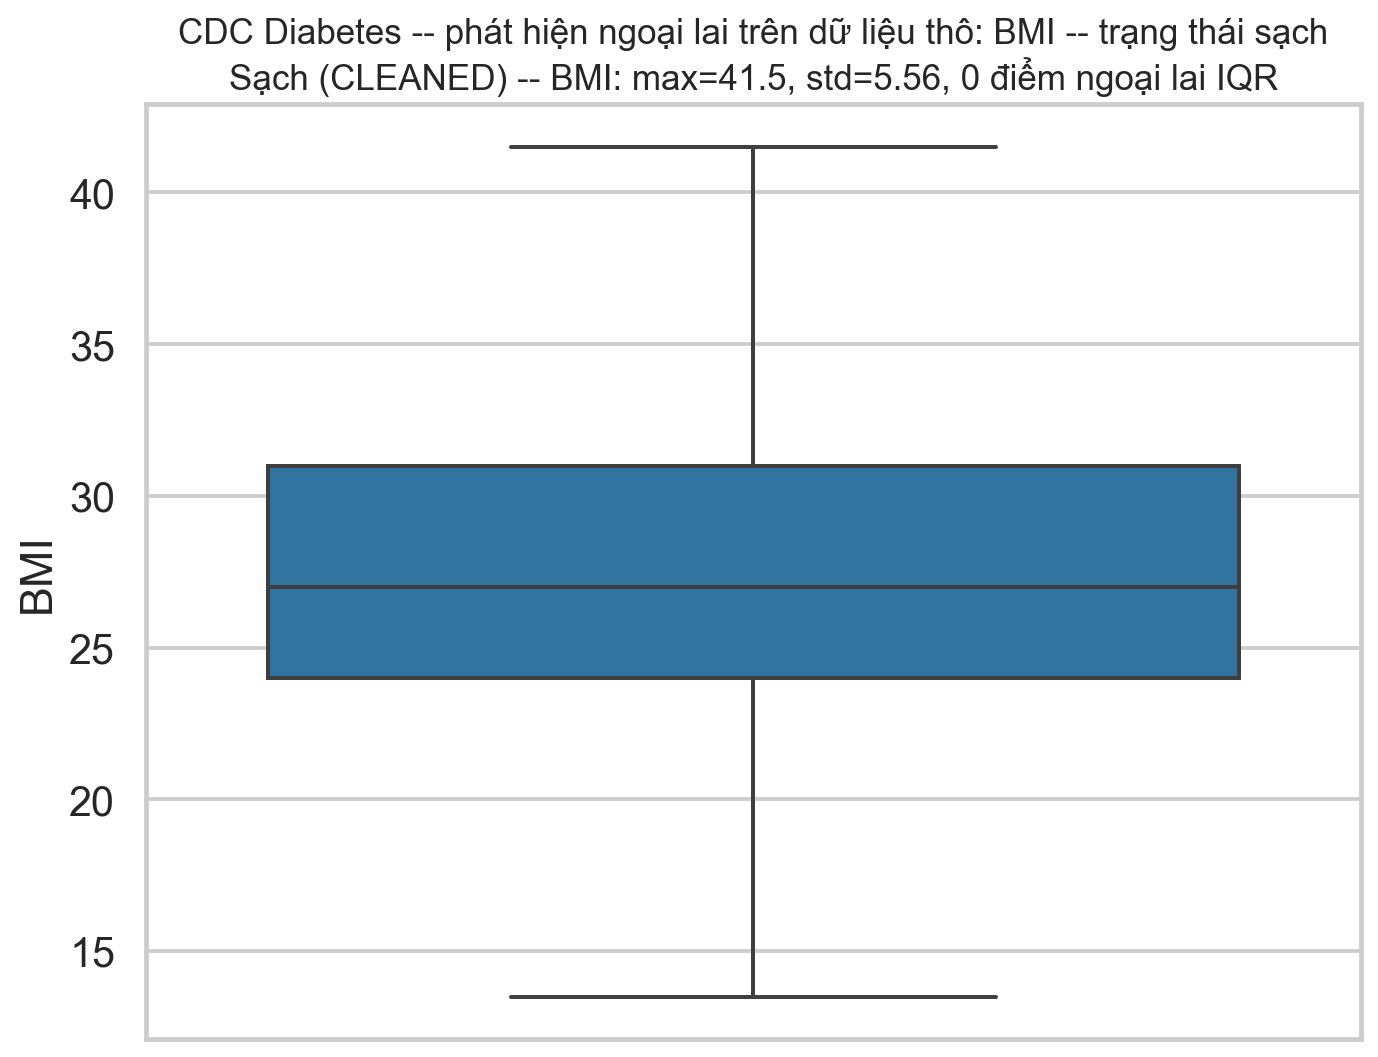
\includegraphics[width=0.72\textwidth]{images/ch3/cdc_diabetes_BMI_boxplot_cleaned.png}
\captionsetup{justification=raggedright,singlelinecheck=false}
\caption[Boxplot \texttt{BMI} sạch CDC Diabetes]{Boxplot \texttt{BMI} CDC Diabetes ở \textbf{trạng thái sạch}: sau clipping IQR, các điểm ngoại lai đuôi phải được nén về ngưỡng trên hộp, max giảm từ 98 xuống $\approx 41.5$.\\
\footnotesize Python source: \texttt{scripts/generate\_raw\_vs\_cleaned\_boxplots.py}.}
\label{fig:ch4_cdc_cleaned_boxplot}
\end{figure}

\textbf{Bước 1. Phân loại biến.}

\begin{table}[H]
\centering
\caption{Bước 1 -- Phân loại biến tiêu biểu trong CDC Diabetes}
\label{tab:ch4_cdc_variable_types}
\small
\begin{tabularx}{\textwidth}{p{0.18\textwidth}p{0.27\textwidth}p{0.25\textwidth}Y}
\toprule
Biến & Bản chất & Thống kê dùng & Biểu đồ phù hợp \\
\midrule
\texttt{BMI} & Quantitative Continuous & Mean, median, IQR, dữ liệu bất thường & Histogram, boxplot \\
\texttt{Age} & Quantitative Discrete/ordinal & Tần suất, median, IQR & Bar chart, scatter \\
\texttt{GenHlth} & Ordinal & Mode, median, IQR & Bar chart, histogram rời rạc \\
\texttt{MentHlth} & Quantitative Discrete & Mean, median, CV & Histogram, boxplot \\
\texttt{PhysHlth} & Quantitative Discrete & Mean, median, CV & Histogram, boxplot \\
\texttt{HighBP} & Qualitative binary & Tần suất, tỷ lệ, mode & Bar chart theo target \\
\bottomrule
\end{tabularx}
\end{table}

Năm biến định lượng/thứ bậc được chọn gồm \texttt{BMI}, \texttt{GenHlth}, \texttt{MentHlth}, \texttt{PhysHlth}, \texttt{Age}; các biến nhị phân \texttt{HighBP}, \texttt{HighChol}, \texttt{PhysActivity}, \texttt{Smoker} được dùng để đọc cấu trúc tần suất và quan hệ với \texttt{Diabetes\_binary}.

\textbf{Bước 2. Bảng tần suất và thống kê mô tả.}

\begin{table}[H]
\centering
\caption[Thống kê mô tả các biến tiêu biểu CDC Diabetes]{Bước 2 -- Thống kê mô tả các biến Quantitative tiêu biểu CDC Diabetes: xu hướng trung tâm và độ phân tán. Source: \texttt{outputs/tables/cdc\_diabetes\_summary.csv}.}
\label{tab:ch4_cdc_stats}
\scriptsize
\setlength{\tabcolsep}{3pt}
\begin{tabular}{lrrrrrrrrrr}
\toprule
Biến & Mean & Med & Mode & P25 & P75 & Range & Var & Std & CV & IQR \\
\midrule
\texttt{BMI} & 28.38 & 27.00 & 27.00 & 24.00 & 31.00 & 86.00 & 43.67 & 6.61 & 0.233 & 7.00 \\
\texttt{GenHlth} & 2.51 & 2.00 & 2.00 & 2.00 & 3.00 & 4.00 & 1.14 & 1.07 & 0.425 & 1.00 \\
\texttt{MentHlth} & 3.18 & 0.00 & 0.00 & 0.00 & 2.00 & 30.00 & 54.95 & 7.41 & 2.328 & 2.00 \\
\texttt{PhysHlth} & 4.24 & 0.00 & 0.00 & 0.00 & 3.00 & 30.00 & 76.00 & 8.72 & 2.055 & 3.00 \\
\texttt{Age} & 8.03 & 8.00 & 9.00 & 6.00 & 10.00 & 12.00 & 9.33 & 3.05 & 0.380 & 4.00 \\
\bottomrule
\end{tabular}
\end{table}

\begin{table}[H]
\centering
\caption[Thống kê thô/sạch CDC Diabetes]{So sánh thống kê mô tả CDC Diabetes ở hai trạng thái: \textbf{thô} và \textbf{sạch} (clipping IQR trên \texttt{BMI}, \texttt{MentHlth}, \texttt{PhysHlth}). Các cột in đậm thay đổi nhiều nhất. Source: \texttt{outputs/tables/cdc\_diabetes\_summary.csv}.}
\label{tab:ch4_cdc_stats_raw_clean}
\footnotesize
\setlength{\tabcolsep}{4pt}
\begin{tabular}{lcrrrrrr}
\toprule
Biến & Trạng thái & Mean & Median & \textbf{Std} & \textbf{Max} & \textbf{Range} & IQR \\
\midrule
\texttt{BMI} & thô & 28.38 & 27.00 & \textbf{6.61} & \textbf{98.00} & \textbf{86.00} & 7.00 \\
 & sạch & 28.11 & 27.00 & \textbf{5.56} & \textbf{41.50} & \textbf{28.00} & 7.00 \\
\midrule
\texttt{GenHlth} & thô & 2.51 & 2.00 & 1.07 & 5.00 & 4.00 & 1.00 \\
 & sạch & 2.51 & 2.00 & 1.07 & 5.00 & 4.00 & 1.00 \\
\midrule
\texttt{MentHlth} & thô & 3.18 & 0.00 & \textbf{7.41} & \textbf{30.00} & \textbf{30.00} & 2.00 \\
 & sạch & 1.18 & 0.00 & \textbf{1.95} & \textbf{5.00} & \textbf{5.00} & 2.00 \\
\midrule
\texttt{PhysHlth} & thô & 4.24 & 0.00 & \textbf{8.72} & \textbf{30.00} & \textbf{30.00} & 3.00 \\
 & sạch & 1.85 & 0.00 & \textbf{2.89} & \textbf{7.50} & \textbf{7.50} & 3.00 \\
\midrule
\texttt{Age} & thô & 8.03 & 8.00 & 3.05 & 13.00 & 12.00 & 4.00 \\
 & sạch & 8.03 & 8.00 & 3.05 & 13.00 & 12.00 & 4.00 \\
\bottomrule
\end{tabular}
\end{table}

\textit{Nhận xét thô/sạch.} CDC Diabetes thể hiện rõ nguyên tắc ``clipping chọn lọc'': \texttt{BMI} giảm std 15.9\% và max 57.7\% (98$\to$41.5); \texttt{MentHlth} và \texttt{PhysHlth} -- hai biến đếm có đuôi dài -- giảm std rất mạnh (73.7\% và 66.9\%) vì phần lớn giá trị cao (gần 30 ngày) bị nén về ngưỡng trên hộp. Trong khi đó \texttt{GenHlth} và \texttt{Age} (ordinal) giữ nguyên mọi chỉ số, do không có ngoại lai trong miền hợp lệ.

\begin{table}[H]
\centering
\caption[Bảng tần suất biến \texttt{HighBP} trong CDC Diabetes]{Bảng tần suất biến \texttt{HighBP} trong CDC Diabetes. Source: \texttt{outputs/tables/cdc\_diabetes\_frequency\_HighBP.csv}.}
\label{tab:ch4_cdc_frequency}
\small
\begin{tabular}{lrr}
\toprule
\texttt{HighBP} & Tần suất tuyệt đối & Tần suất tương đối \\
\midrule
0 (không huyết áp cao) & 144\,851 & 57.10\% \\
1 (có huyết áp cao) & 108\,829 & 42.90\% \\
\bottomrule
\end{tabular}
\end{table}

\textbf{Bước 3. Trực quan hóa dữ liệu.} Tương tự Heart Disease, hệ thống biểu đồ của CDC Diabetes được chọn theo bản chất biến: bar chart cho biến nhị phân \texttt{HighBP}, histogram và boxplot cho \texttt{BMI}, scatter plot cho quan hệ \texttt{Age}--\texttt{BMI}, biểu đồ phân bố target để kiểm tra mất cân bằng lớp và heatmap để khảo sát tương quan giữa các yếu tố nguy cơ chuyển hóa.

\begin{figure}[H]
\centering
\begin{subfigure}{0.90\textwidth}
 \centering
 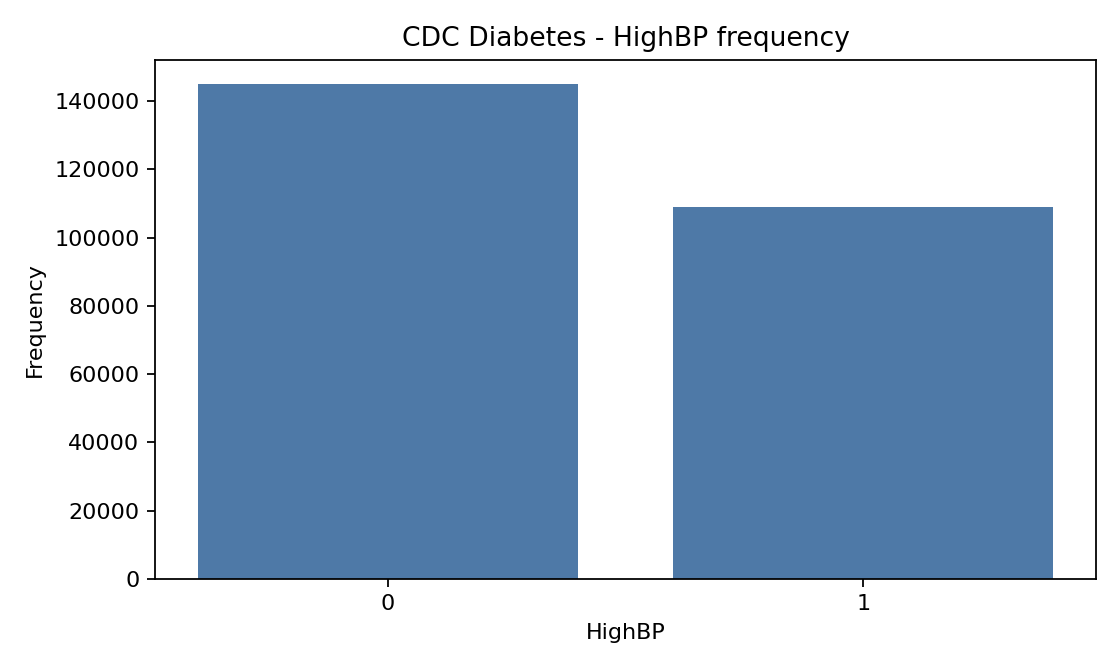
\includegraphics[width=\textwidth]{images/ch3/cdc_diabetes_highbp_bar.png}
 \caption{Python -- Bar chart \texttt{HighBP}}
\end{subfigure}
\par\medskip
\begin{subfigure}{0.90\textwidth}
 \centering
 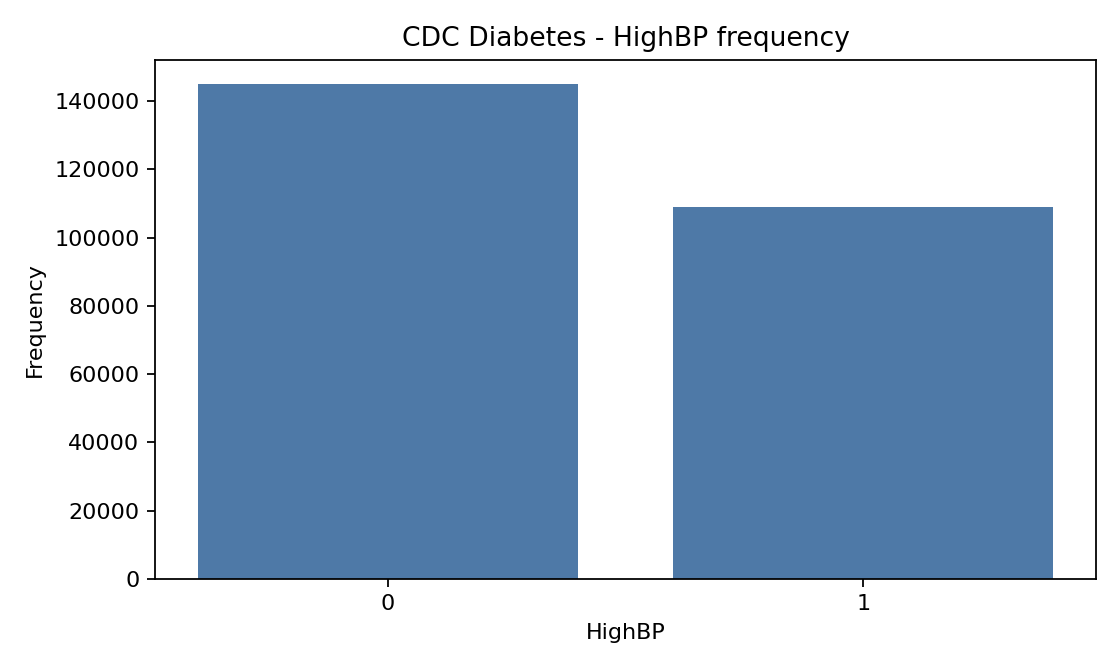
\includegraphics[width=\textwidth]{images/ch3/excel_cdc_highbp_bar_preview.png}
 \caption{Excel -- Column chart \texttt{HighBP}}
\end{subfigure}
\captionsetup{justification=raggedright,singlelinecheck=false}
\caption[Bar chart \texttt{HighBP} CDC Diabetes: Python và Excel]{Tần suất huyết áp cao trong CDC Diabetes, đối chiếu giữa Python và Excel.\\
\footnotesize Python source: \texttt{src/analyze\_cdc\_diabetes.py}.\\
Excel source/workbook: \texttt{src/create\_excel\_visualizations.py}, \texttt{excel/excel\_visualization\_comparison\_native.xlsx}, sheet \texttt{CDC HighBP}.}
\label{fig:ch4_cdc_highbp_bar}
\end{figure}

\textbf{Nhận xét Hình \ref{fig:ch4_cdc_highbp_bar}.} Biến \texttt{HighBP} có tỷ lệ có huyết áp cao 42.90\%, đủ lớn để trở thành tín hiệu nguy cơ quan trọng. Vì đây là biến nhị phân định tính, tần suất tuyệt đối, tần suất tương đối và mode phù hợp hơn mean/median.

\begin{figure}[H]
\centering
\begin{subfigure}{0.90\textwidth}
 \centering
 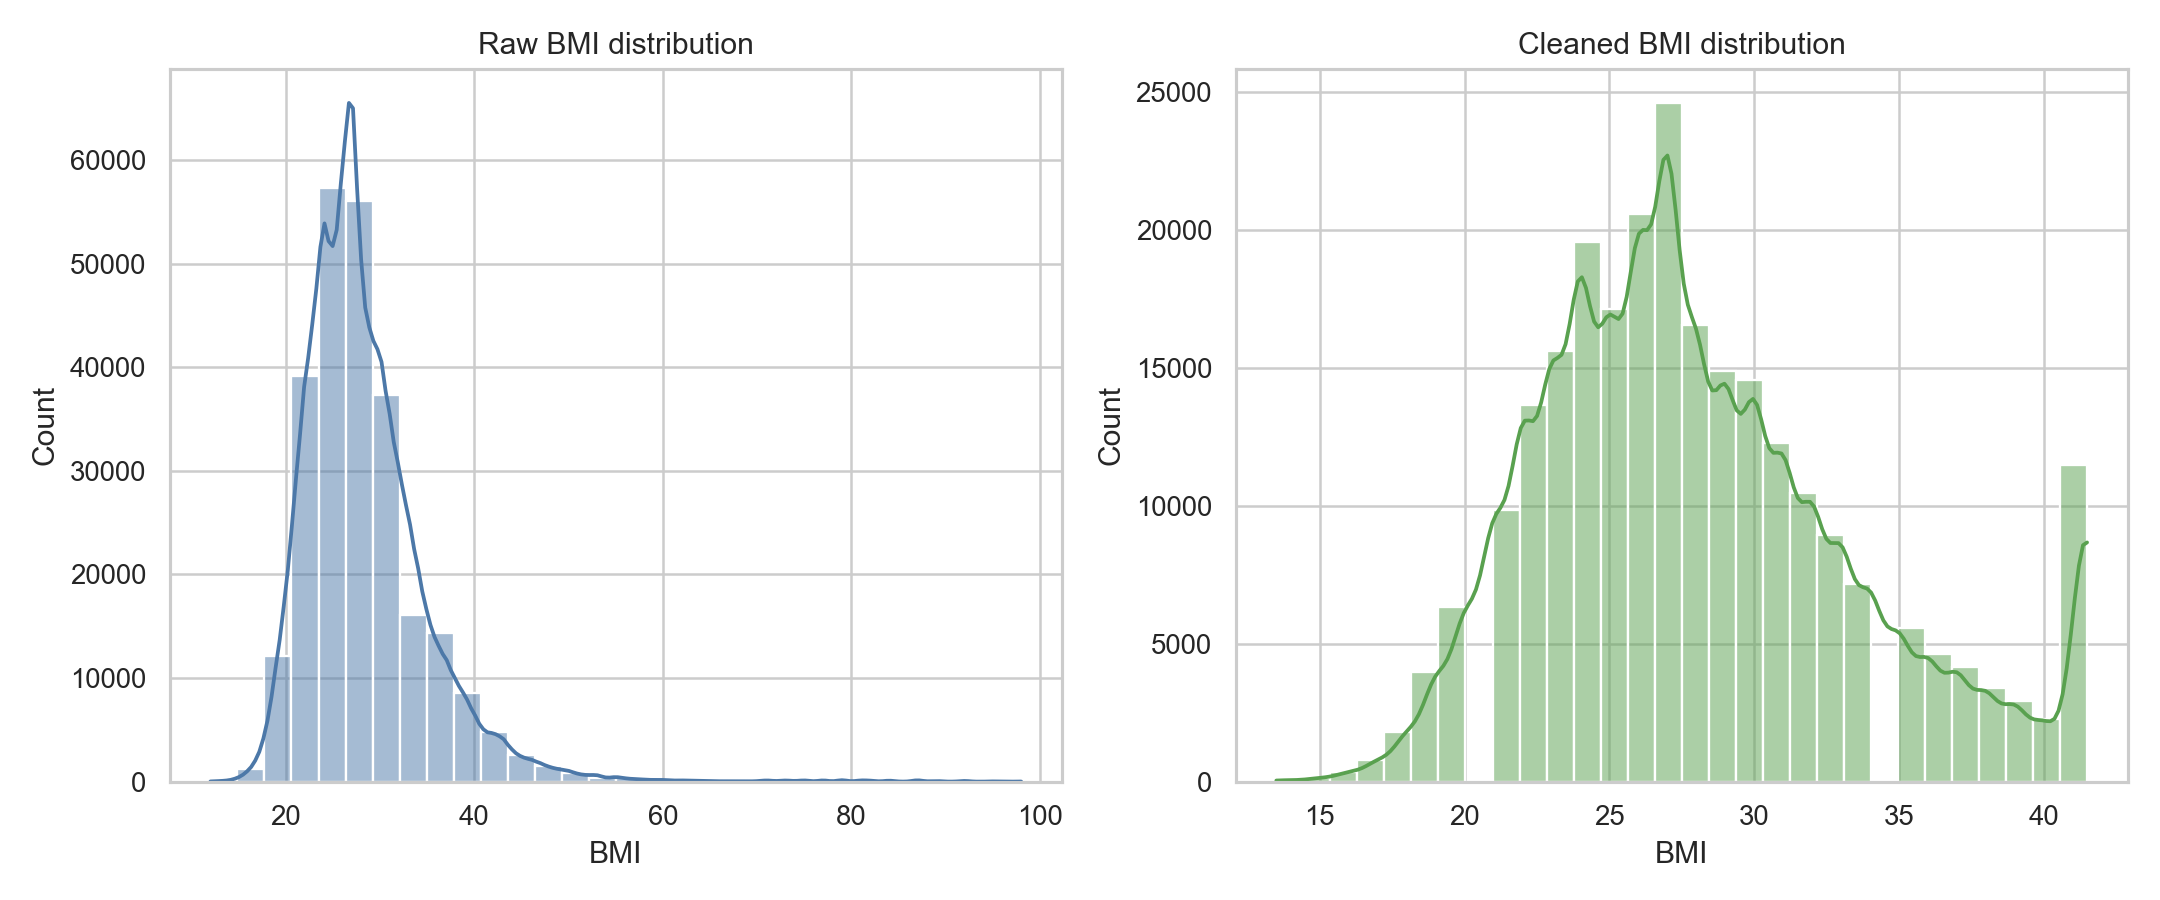
\includegraphics[width=\textwidth]{images/ch3/cdc_diabetes_bmi_raw_vs_cleaned.png}
 \caption{Python -- Histogram \texttt{BMI} thô/sạch}
\end{subfigure}
\par\medskip
\begin{subfigure}{0.90\textwidth}
 \centering
 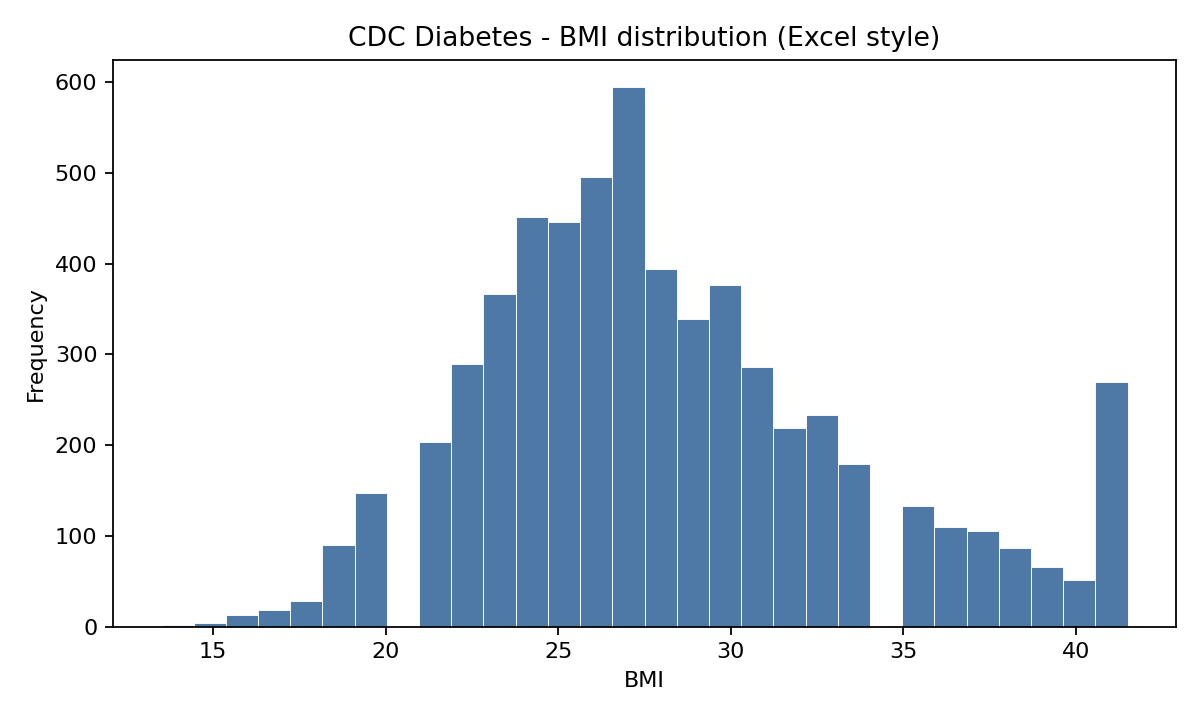
\includegraphics[width=\textwidth]{images/ch3/excel_cdc_bmi_raw_vs_cleaned_preview.png}
 \caption{Excel -- Histogram \texttt{BMI}}
\end{subfigure}
\captionsetup{justification=raggedright,singlelinecheck=false}
\caption[Histogram \texttt{BMI} CDC Diabetes: Python và Excel]{Phân phối \texttt{BMI} sau tiền xử lý trong CDC Diabetes, đối chiếu giữa Python và Excel.\\
\footnotesize Python source: \texttt{src/analyze\_cdc\_diabetes.py}.\\
Excel source/workbook: \texttt{src/create\_excel\_visualizations.py}, \texttt{excel/excel\_visualization\_comparison\_native.xlsx}, sheet \texttt{CDC BMI Hist}.}
\label{fig:ch4_cdc_bmi_hist}
\end{figure}

\textbf{Nhận xét Hình \ref{fig:ch4_cdc_bmi_hist}.} Histogram \texttt{BMI} cho thấy tiền xử lý làm đuôi phải ngắn hơn: max giảm từ 98 xuống 41.5 và độ lệch chuẩn giảm từ 6.61 xuống 5.56. Như vậy dữ liệu sau xử lý có phân phối mượt và ít bị chi phối bởi vài quan sát cực trị hơn dữ liệu thô.

\begin{figure}[H]
\centering
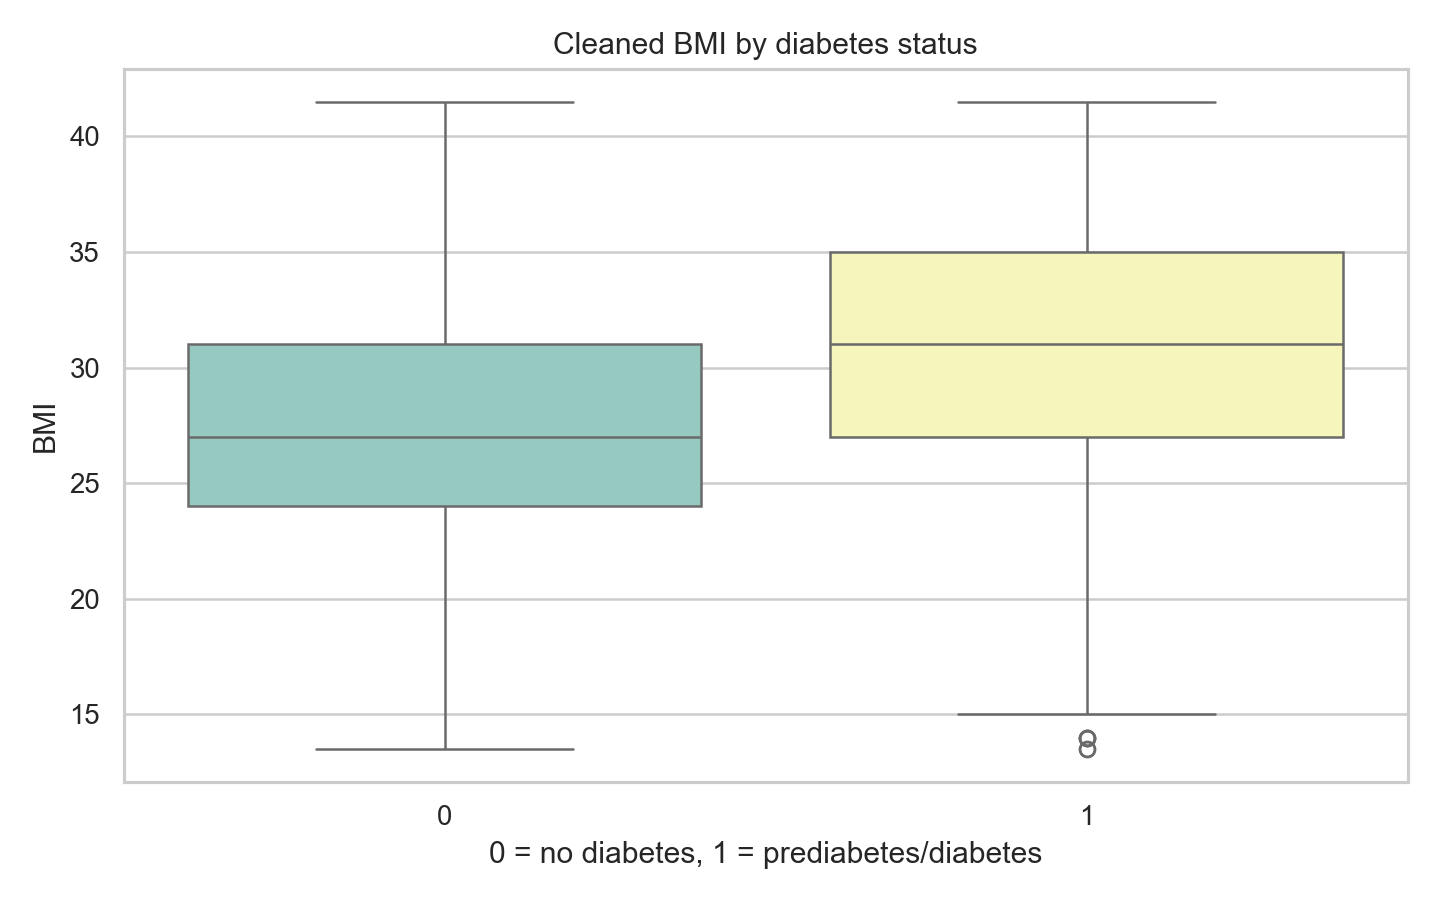
\includegraphics[width=0.90\textwidth]{images/ch3/cdc_diabetes_bmi_boxplot_by_target.png}
\captionsetup{justification=raggedright,singlelinecheck=false}
\caption[Boxplot \texttt{BMI} CDC Diabetes]{Boxplot \texttt{BMI} theo \texttt{Diabetes\_binary}.\\
\footnotesize Python source: \texttt{src/analyze\_cdc\_diabetes.py}.}
\label{fig:ch4_cdc_bmi_boxplot}
\end{figure}

\textbf{Nhận xét Hình \ref{fig:ch4_cdc_bmi_boxplot}.} Nhóm có tiểu đường có trung vị \texttt{BMI} cao hơn, dù hai hộp vẫn chồng lấn nhiều. Điều này cho thấy \texttt{BMI} có tín hiệu nhưng không đủ để phân loại đơn biến.

\textit{Đối chiếu thô/sạch.} Hai biểu đồ tiếp theo đặt dữ liệu thô (đỏ) cạnh dữ liệu sạch (xanh), qua đó thể hiện trực quan tác động của clipping IQR trên \texttt{BMI}.

\begin{figure}[H]
\centering
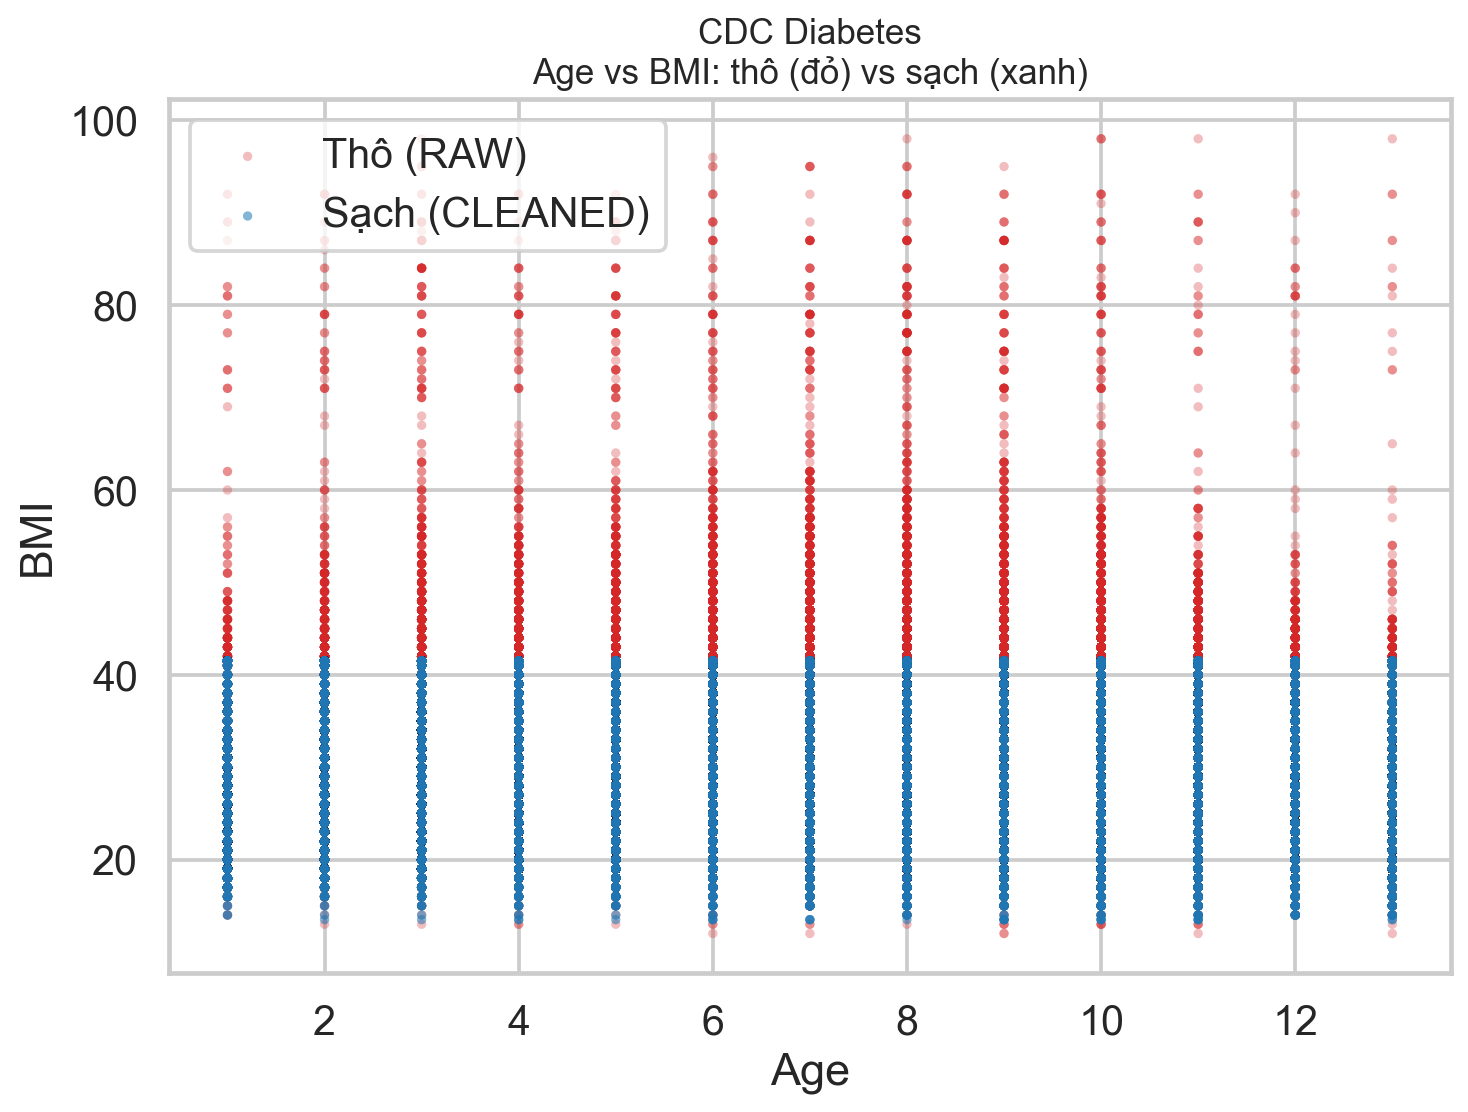
\includegraphics[width=0.82\textwidth]{images/ch3/cdc_diabetes_age_bmi_scatter_raw_vs_cleaned.png}
\captionsetup{justification=raggedright,singlelinecheck=false}
\caption[Scatter \texttt{Age}--\texttt{BMI} thô/sạch CDC Diabetes]{Scatter \texttt{Age}--\texttt{BMI} CDC Diabetes: dữ liệu thô (đỏ, mờ) phủ rộng tới BMI=98; dữ liệu sạch (xanh) bị nén về $\approx$41.5 -- vùng trên bị cắt rõ.\\
\footnotesize Python source: \texttt{scripts/generate\_raw\_vs\_cleaned\_boxplots.py}.}
\label{fig:ch4_cdc_scatter_compare}
\end{figure}

\begin{figure}[H]
\centering
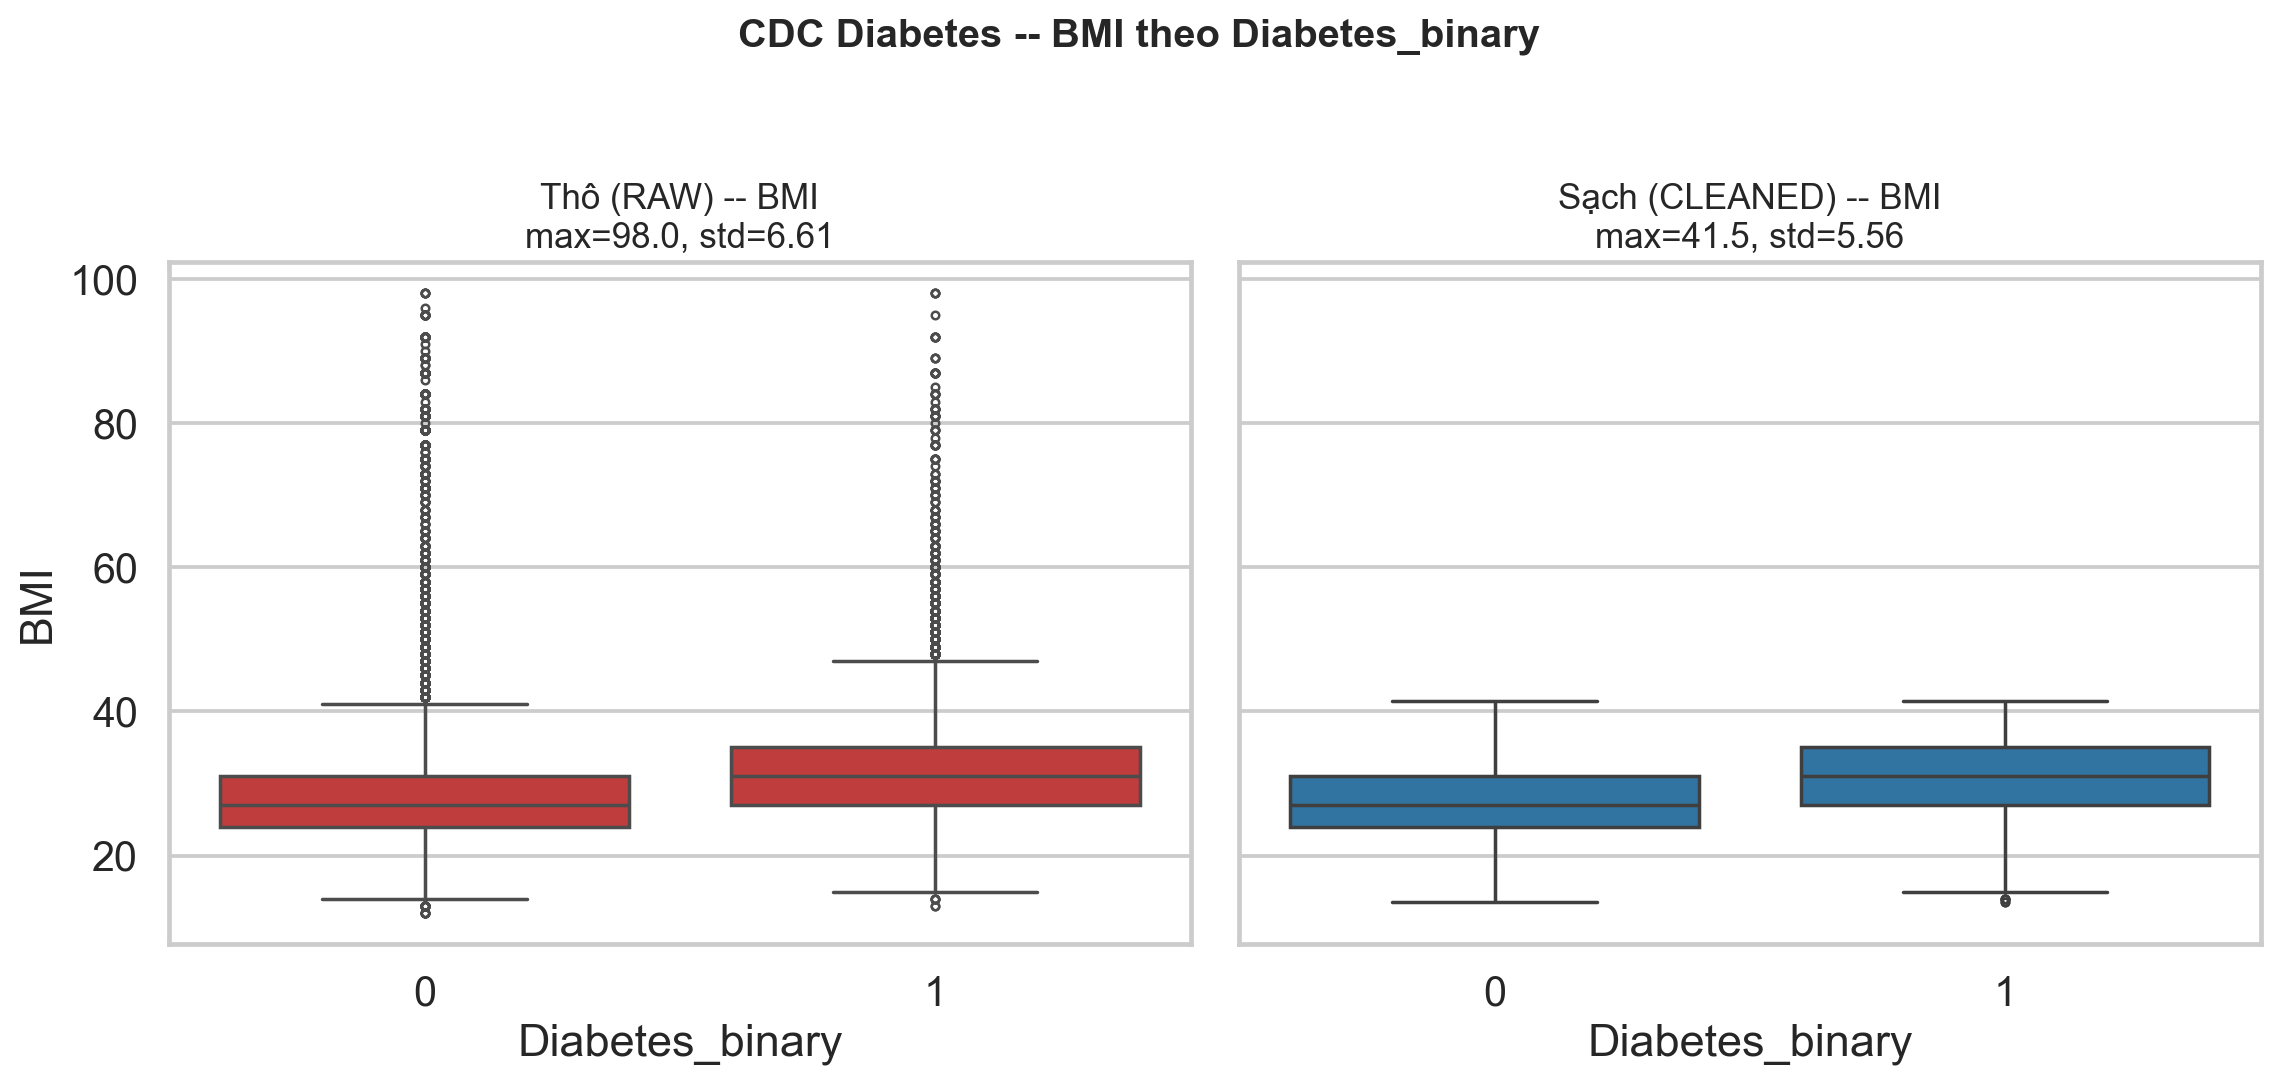
\includegraphics[width=0.95\textwidth]{images/ch3/cdc_diabetes_BMI_boxplot_by_target_raw_vs_cleaned.png}
\captionsetup{justification=raggedright,singlelinecheck=false}
\caption[Boxplot \texttt{BMI} theo target thô/sạch CDC Diabetes]{Boxplot \texttt{BMI} theo \texttt{Diabetes\_binary}: thô (trái) có hàng nghìn điểm ngoại lai tới 98; sạch (phải) sau clipping giảm ngoại lai nhưng trung vị nhóm tiểu đường vẫn cao hơn.\\
\footnotesize Python source: \texttt{scripts/generate\_raw\_vs\_cleaned\_boxplots.py}.}
\label{fig:ch4_cdc_boxplot_by_target_compare}
\end{figure}

\textbf{Nhận xét.} Scatter \texttt{Age}--\texttt{BMI} (Hình~\ref{fig:ch4_cdc_scatter_compare}) cho thấy vùng BMI$>$41.5 của dữ liệu thô (đỏ) biến mất ở dữ liệu sạch (xanh), nhưng phần lõi phân bố vẫn trùng nhau. Boxplot theo target (Hình~\ref{fig:ch4_cdc_boxplot_by_target_compare}) xác nhận sau clipping, hàng nghìn điểm ngoài râu bị nén, nhưng trung vị nhóm tiểu đường vẫn cao hơn nhóm không tiểu đường -- tín hiệu nguy cơ chuyển hóa được giữ nguyên.

\begin{figure}[H]
\centering
\begin{subfigure}{0.90\textwidth}
 \centering
 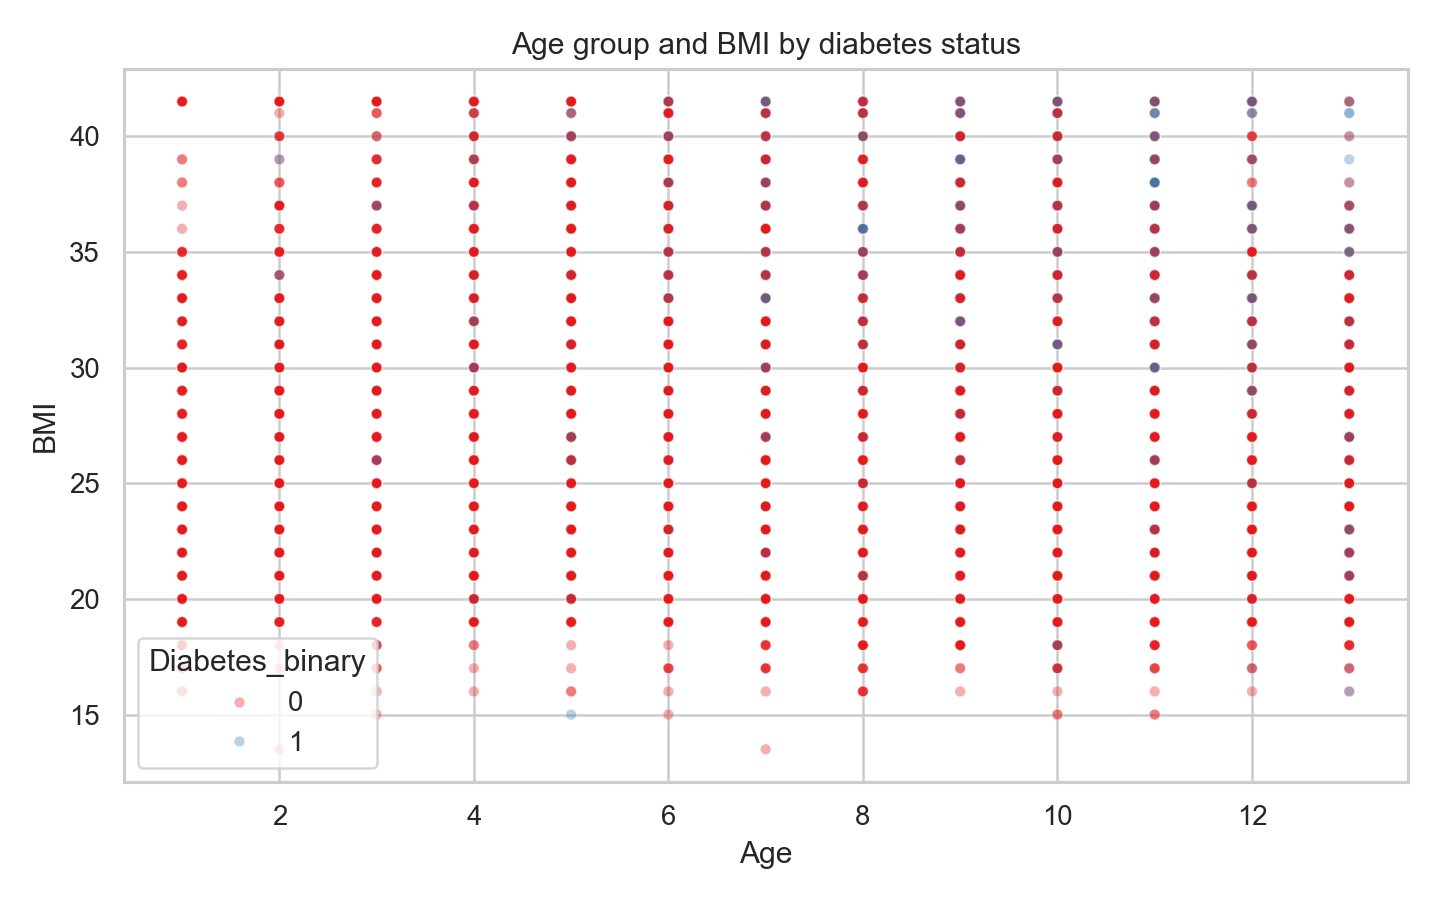
\includegraphics[width=\textwidth]{images/ch3/cdc_diabetes_age_bmi_scatter.png}
 \caption{Python -- Scatter \texttt{Age}--\texttt{BMI}}
\end{subfigure}
\par\medskip
\begin{subfigure}{0.90\textwidth}
 \centering
 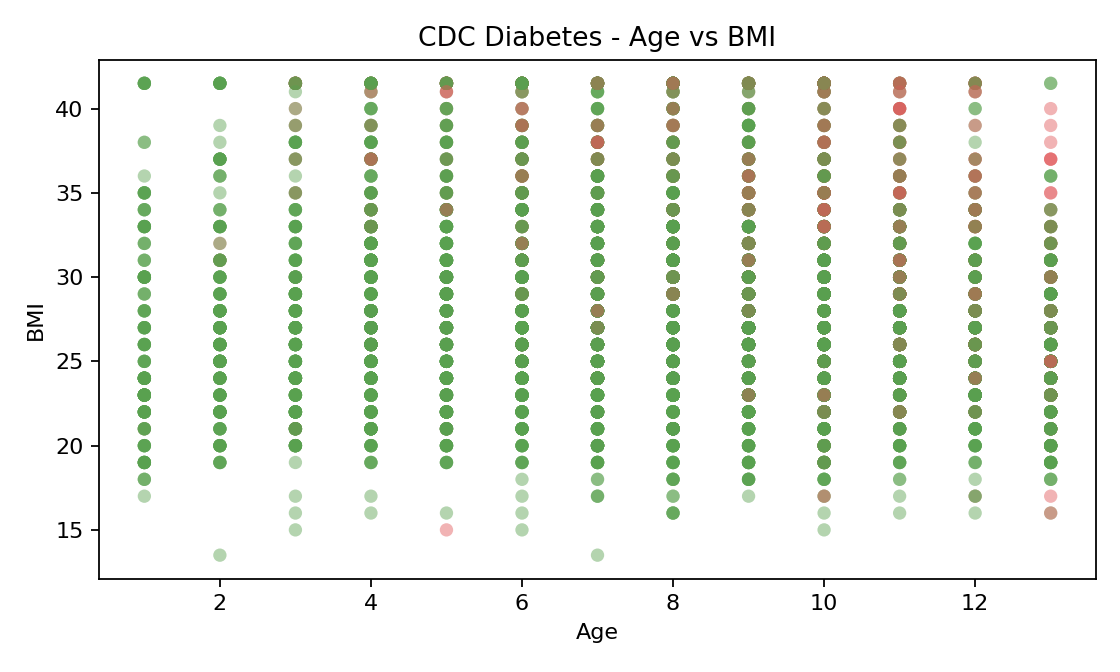
\includegraphics[width=\textwidth]{images/ch3/excel_cdc_age_bmi_scatter_preview.png}
 \caption{Excel -- Scatter \texttt{Age}--\texttt{BMI}}
\end{subfigure}
\captionsetup{justification=raggedright,singlelinecheck=false}
\caption[Scatter \texttt{Age}--\texttt{BMI} CDC Diabetes: Python và Excel]{Quan hệ giữa nhóm tuổi và BMI trong CDC Diabetes.\\
\footnotesize Python source: \texttt{src/analyze\_cdc\_diabetes.py}.\\
Excel source/workbook: \texttt{src/create\_excel\_visualizations.py}, \texttt{excel/excel\_visualization\_comparison\_native.xlsx}, sheet \texttt{CDC Age BMI}.}
\label{fig:ch4_cdc_age_bmi}
\end{figure}

\textbf{Nhận xét Hình \ref{fig:ch4_cdc_age_bmi}.} Scatter \texttt{Age}--\texttt{BMI} cho thấy dữ liệu phủ rộng ở nhiều nhóm tuổi; BMI cao xuất hiện ở nhiều mức tuổi thay vì chỉ tập trung ở một nhóm.

\begin{figure}[H]
\centering
\begin{subfigure}{0.90\textwidth}
 \centering
 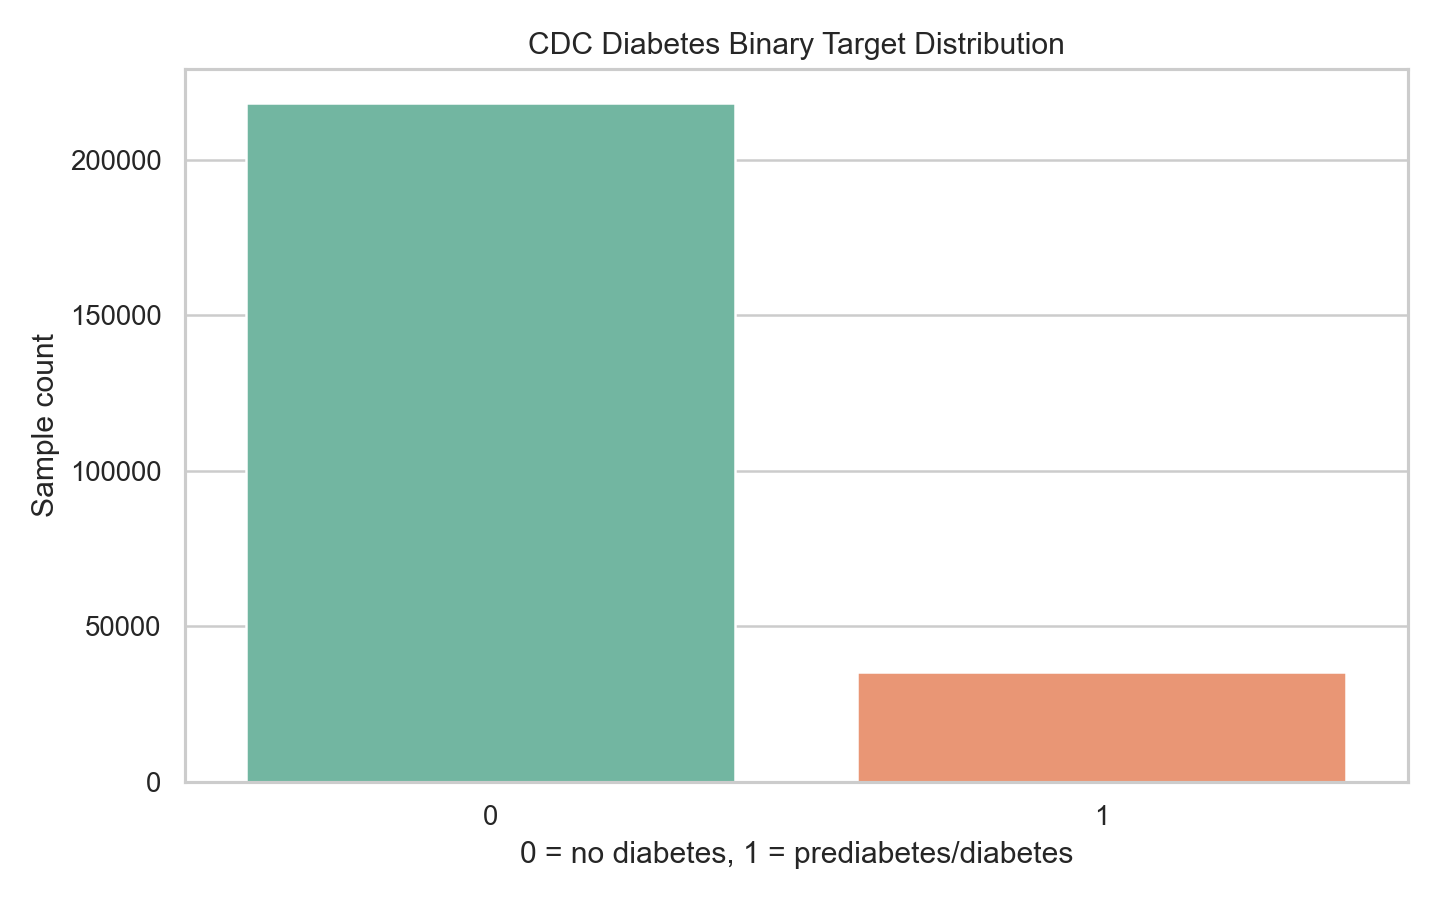
\includegraphics[width=\textwidth]{images/ch3/cdc_diabetes_target_distribution.png}
 \caption{Python -- Phân bố \texttt{Diabetes\_binary}}
\end{subfigure}
\par\medskip
\begin{subfigure}{0.90\textwidth}
 \centering
 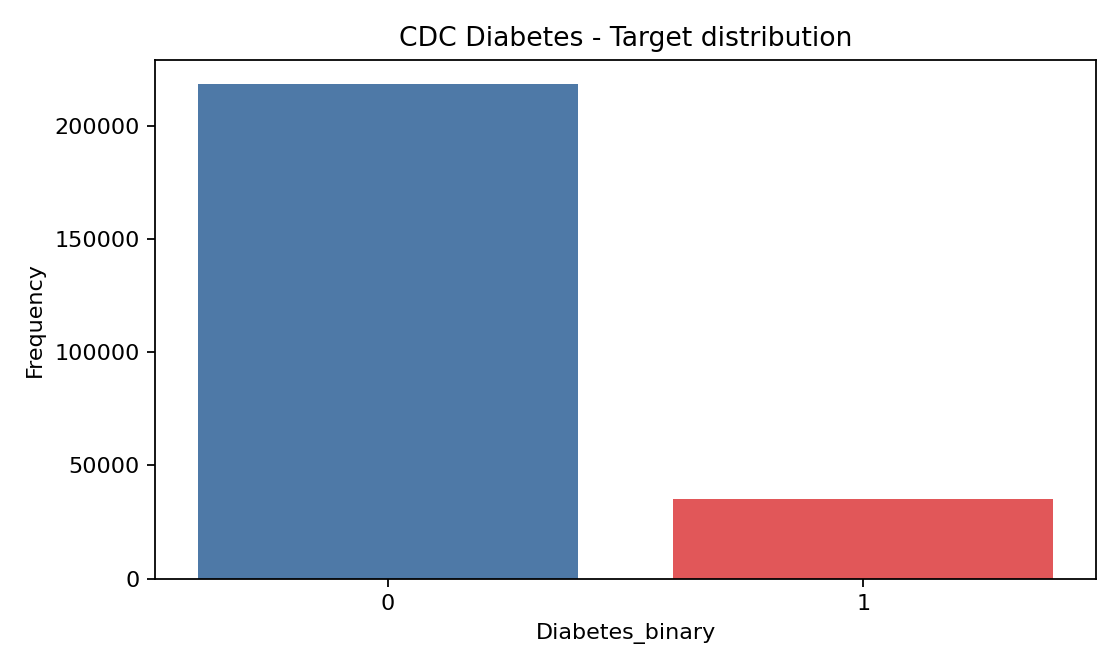
\includegraphics[width=\textwidth]{images/ch3/excel_cdc_target_distribution_preview.png}
 \caption{Excel -- Phân bố \texttt{Diabetes\_binary}}
\end{subfigure}
\captionsetup{justification=raggedright,singlelinecheck=false}
\caption[Phân bố target CDC Diabetes: Python và Excel]{Phân bố biến mục tiêu \texttt{Diabetes\_binary}, đối chiếu giữa Python và Excel.\\
\footnotesize Python source: \texttt{src/analyze\_cdc\_diabetes.py}.\\
Excel source/workbook: \texttt{src/create\_excel\_visualizations.py}, \texttt{excel/excel\_visualization\_comparison\_native.xlsx}, sheet \texttt{CDC Target}.}
\label{fig:ch4_cdc_target}
\end{figure}

\textbf{Nhận xét Hình \ref{fig:ch4_cdc_target}.} Phân bố target cho thấy lớp không tiểu đường chiếm ưu thế, dữ liệu mất cân bằng rõ rệt. Vì vậy, accuracy không đủ để đánh giá mô hình phân loại; cần đọc kèm precision, recall và F1, đặc biệt cho lớp tiểu đường.

\begin{figure}[H]
\centering
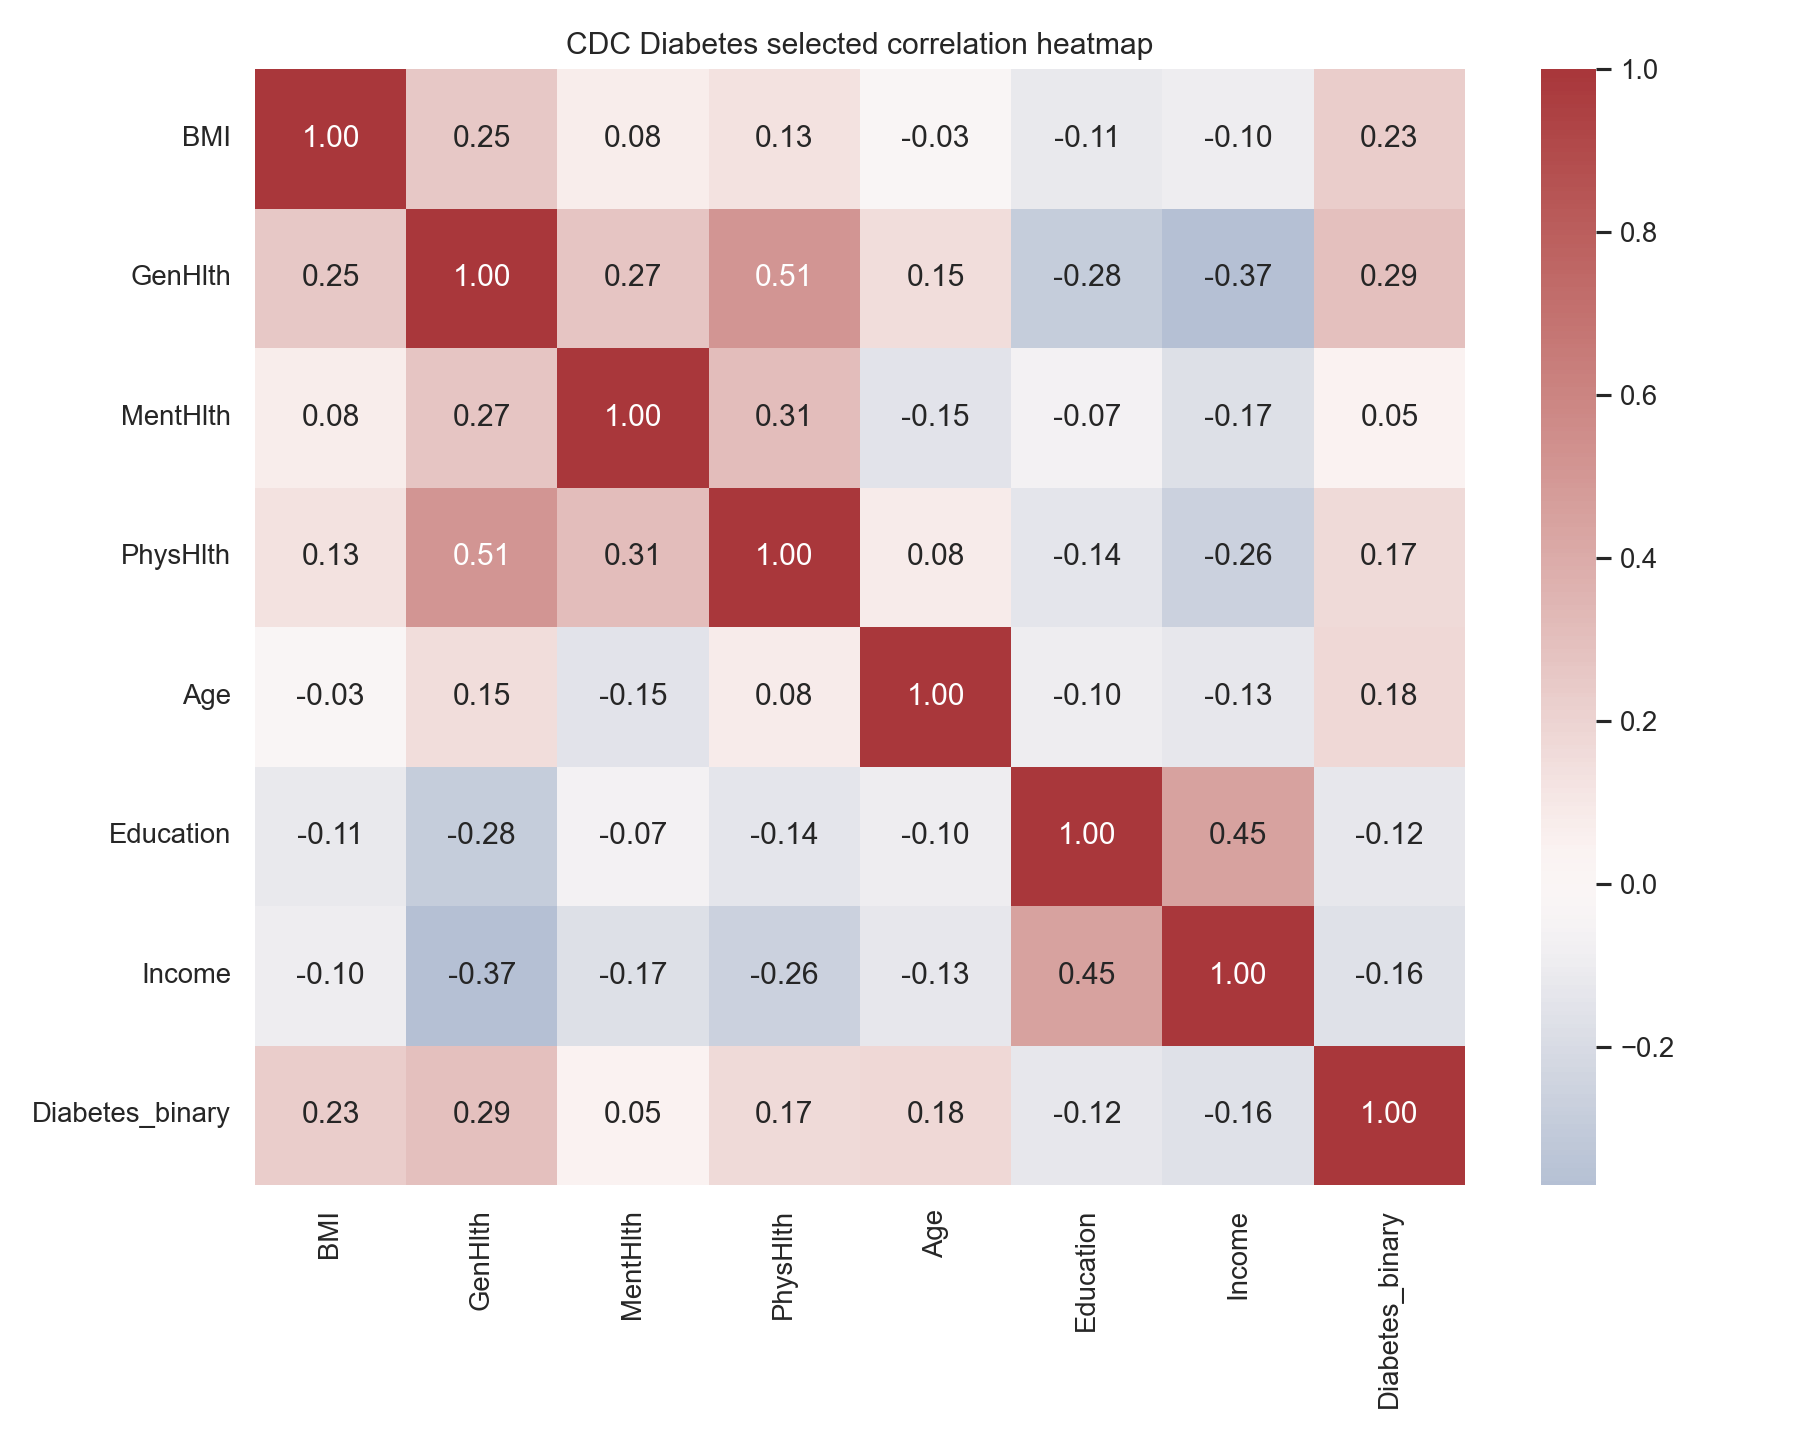
\includegraphics[width=0.86\textwidth]{images/ch3/cdc_diabetes_correlation_heatmap.png}
\captionsetup{justification=raggedright,singlelinecheck=false}
\caption[Heatmap tương quan CDC Diabetes]{Heatmap tương quan các biến CDC Diabetes.\\
\footnotesize Python source: \texttt{src/analyze\_cdc\_diabetes.py}.}
\label{fig:ch4_cdc_corr}
\end{figure}

\textbf{Nhận xét Hình \ref{fig:ch4_cdc_corr}.} Heatmap tương quan cho thấy nhóm \texttt{HighBP}, \texttt{HighChol}, \texttt{GenHlth} và \texttt{BMI} mô tả các khía cạnh khác nhau của nguy cơ chuyển hóa. Các tương quan không quá cao tuyệt đối, vì vậy từng biến vẫn có thể đóng góp thông tin riêng cho mô hình đa biến.

\textbf{Nhận xét về hình dáng phân phối.} \texttt{BMI}, \texttt{MentHlth} và \texttt{PhysHlth} đều lệch phải. Với \texttt{MentHlth} và \texttt{PhysHlth}, median và mode đều bằng 0 trong khi max đạt 30 ngày, cho thấy phần lớn người trả lời không ghi nhận ngày sức khỏe kém nhưng vẫn tồn tại một nhóm nhỏ có gánh nặng sức khỏe cao. Với \texttt{BMI}, mean lớn hơn median và đuôi phải dài, phản ánh một nhóm quan sát béo phì mức cao cần được kiểm soát bằng clipping trước khi mô hình hóa.

\textbf{Bước 4. So sánh trước--sau tiền xử lý.} Bảng~\ref{tab:ch4_cdc_preprocess} đặt các chỉ số của trạng thái thô cạnh trạng thái sạch; các hình thô/sạch ở trên minh họa trực tiếp tác động của clipping IQR.

\begin{table}[H]
\centering
\caption[So sánh dữ liệu thô và sạch CDC Diabetes]{Bước 4 -- So sánh dữ liệu thô và dữ liệu sạch CDC Diabetes (clipping IQR trên \texttt{BMI}, \texttt{MentHlth}, \texttt{PhysHlth}; 0 ô khuyết ở cả hai trạng thái). Source: \texttt{outputs/tables/cdc\_diabetes\_preprocessing\_comparison.csv}.}
\label{tab:ch4_cdc_preprocess}
\small
\begin{tabular}{lrrrrrr}
\toprule
Biến & Mean thô & Mean sạch & Std thô & Std sạch & Max thô & Max sạch \\
\midrule
\texttt{BMI} & 28.38 & 28.11 & 6.61 & 5.56 & 98.0 & 41.5 \\
\texttt{GenHlth} & 2.51 & 2.51 & 1.07 & 1.07 & 5.0 & 5.0 \\
\texttt{MentHlth} & 3.18 & 1.18 & 7.41 & 1.95 & 30.0 & 5.0 \\
\texttt{PhysHlth} & 4.24 & 1.85 & 8.72 & 2.89 & 30.0 & 7.5 \\
\texttt{Age} & 8.03 & 8.03 & 3.05 & 3.05 & 13.0 & 13.0 \\
\bottomrule
\end{tabular}
\end{table}

Bảng~\ref{tab:ch4_cdc_preprocess} cho thấy clipping IQR ảnh hưởng mạnh đến ba biến có ngoại lai và không làm thay đổi các biến ordinal đã sạch. Cụ thể, \texttt{BMI} giảm standard deviation 15.9\% (6.61$\to$5.56) và max giảm 57.7\% (98$\to$41.5); \texttt{MentHlth} giảm standard deviation 73.7\% (7.41$\to$1.95), còn \texttt{PhysHlth} giảm 66.9\% (8.72$\to$2.89). Trong khi đó, \texttt{GenHlth} và \texttt{Age} giữ nguyên mean, standard deviation và max vì các giá trị đã nằm trong miền hợp lệ.

\textbf{Kết luận cho CDC Diabetes.} Có ba kết quả chính rút ra từ phân tích. Thứ nhất, bộ dữ liệu không có ô khuyết, nên tiền xử lý tập trung vào ngoại lai thay vì điền khuyết. Thứ hai, clipping được áp dụng có chọn lọc cho \texttt{BMI}, \texttt{MentHlth} và \texttt{PhysHlth}, giúp giảm ảnh hưởng của đuôi phải cực trị nhưng vẫn giữ nguyên phần lõi phân phối. Thứ ba, biến mục tiêu mất cân bằng rõ rệt, do đó các phân tích và mô hình học máy cần ưu tiên metric theo lớp thay vì chỉ dựa vào accuracy.

\subsubsection{Breast Cancer Wisconsin Diagnostic}

Breast Cancer Wisconsin Diagnostic có 569 quan sát, 30 đặc trưng hình thái định lượng liên tục được trích xuất từ ảnh tế bào và biến mục tiêu \texttt{Diagnosis} gồm hai lớp B/M (lành tính/ác tính). Trong mục này, sáu biến đại diện được chọn là \texttt{radius1}, \texttt{texture1}, \texttt{perimeter1}, \texttt{area1}, \texttt{smoothness1} và \texttt{concavity1}. Nhóm biến này bao quát kích thước, bề mặt và độ lõm của khối u, do đó phù hợp để minh họa thống kê mô tả, trực quan hóa và đánh giá tác động của xử lý ngoại lai.

\textbf{Trạng thái dữ liệu thô.} Trước khi tính toán thống kê, dữ liệu được kiểm tra ô khuyết và giá trị ngoại lai. Breast Cancer \emph{không có ô khuyết thiếu} (0/569 dòng, theo \texttt{outputs/tables/breast\_cancer\_missing\_values.csv}), nên không cần điền khuyết. Đặc điểm cần chú ý là các đặc trưng hình thái có \emph{thang đo rất khác nhau}: \texttt{area1} có range xấp xỉ 2357, lớn hơn nhiều so với các biến như \texttt{smoothness1} hoặc \texttt{concavity1} có range nhỏ hơn 1.

\begin{figure}[H]
\centering
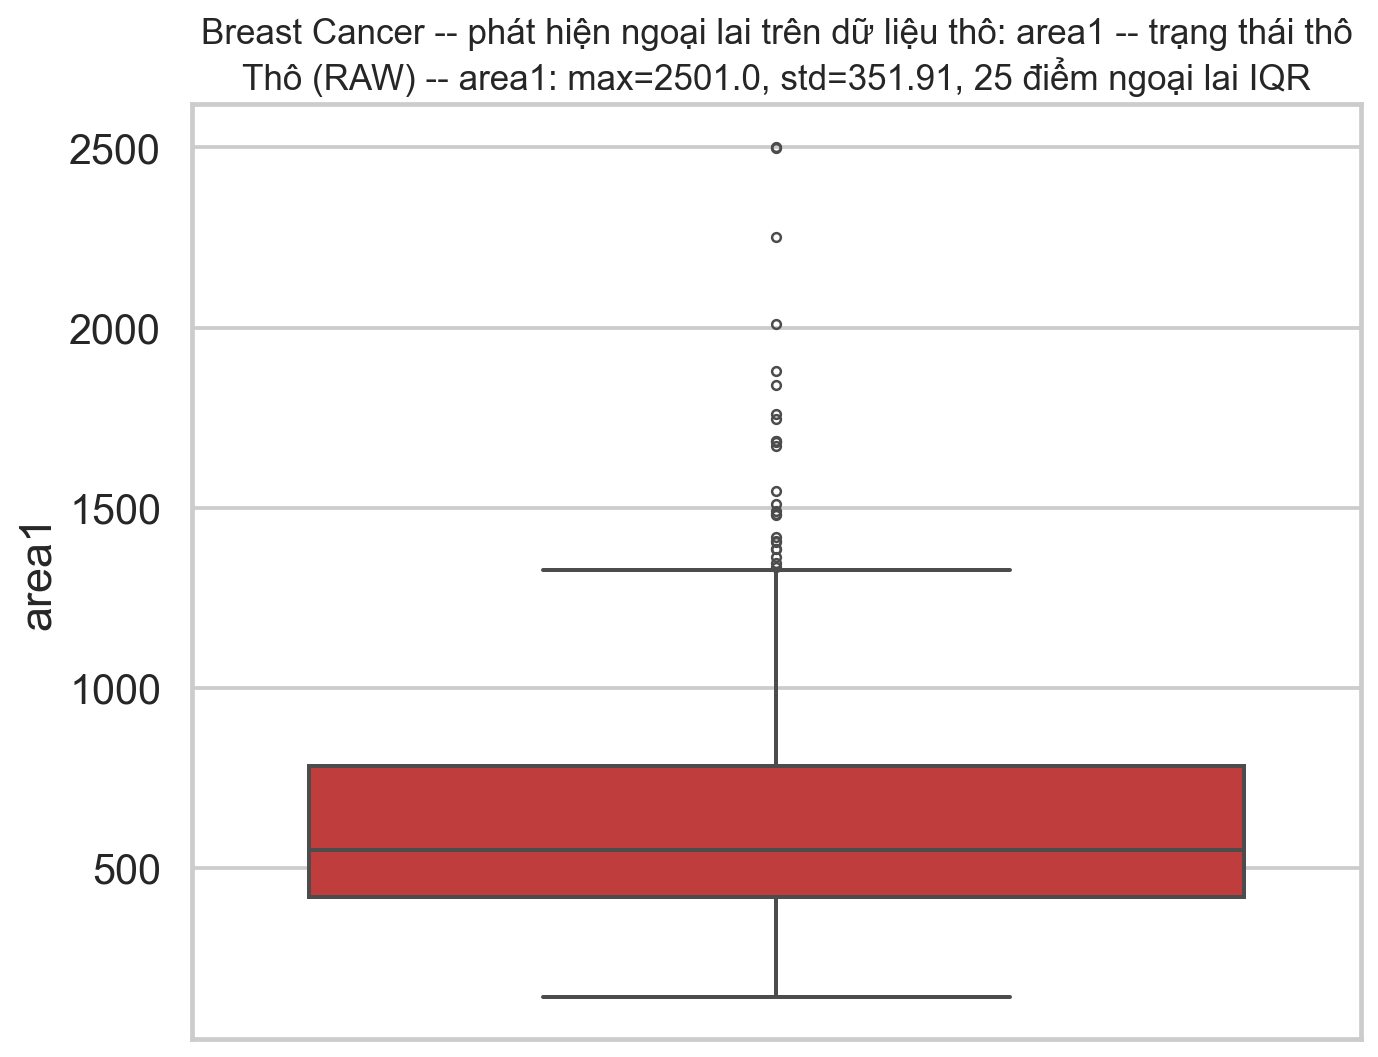
\includegraphics[width=0.72\textwidth]{images/ch3/breast_cancer_area1_boxplot_raw.png}
\captionsetup{justification=raggedright,singlelinecheck=false}
\caption[Boxplot \texttt{area1} thô Breast Cancer]{Boxplot \texttt{area1} Breast Cancer ở \textbf{trạng thái thô}: nhiều điểm ngoại lai tới $\sim$2501 (median 551), tập trung ở nhóm ác tính (M).\\
\footnotesize Python source: \texttt{scripts/generate\_raw\_vs\_cleaned\_boxplots.py}.}
\label{fig:ch4_breast_raw_boxplot}
\end{figure}

\textit{Phát hiện ngoại lai trên dữ liệu thô.} Hình~\ref{fig:ch4_breast_raw_boxplot} cho thấy một số ca khối u lớn tạo điểm rời rạc ở đuôi phải. \texttt{radius1} có các giá trị vượt 25 so với median 13.37; \texttt{perimeter1} đạt xấp xỉ 188; đặc biệt, \texttt{area1} đạt xấp xỉ 2501 trong khi median chỉ 551. Các điểm xa râu hộp này tập trung nhiều ở nhóm ác tính (M). Ngoài ra, \texttt{concavity1} lệch phải rõ với mode bằng 0 và một số ca đạt 0.427. Vì nhiều ngoại lai có thể phản ánh khối u ác tính kích thước lớn, clipping cần được áp dụng thận trọng thay vì loại bỏ cơ học.

\textbf{Làm sạch dữ liệu.} Quy trình tiền xử lý được thực hiện theo ba nguyên tắc sau:

\begin{itemize}[leftmargin=*]
    \item \textbf{Điền khuyết:} \emph{không cần} -- dữ liệu thô không có ô NaN.
    \item \textbf{Xử lý ngoại lai:} \emph{clipping theo quy tắc IQR} trên sáu biến được chọn \texttt{radius1}, \texttt{texture1}, \texttt{perimeter1}, \texttt{area1}, \texttt{smoothness1}, \texttt{concavity1}. Cách xử lý này nén giá trị cực trị về biên hộp nhưng vẫn giữ quan sát trong tập dữ liệu.
    \item \textbf{Chuẩn hóa:} \emph{chưa áp dụng} ở giai đoạn thống kê mô tả để giữ đơn vị hình thái gốc; Min--Max Scaling hoặc Z-score chỉ được dùng ở chương học máy khi cần đưa các đặc trưng về cùng thang đo.
\end{itemize}

\begin{figure}[H]
\centering
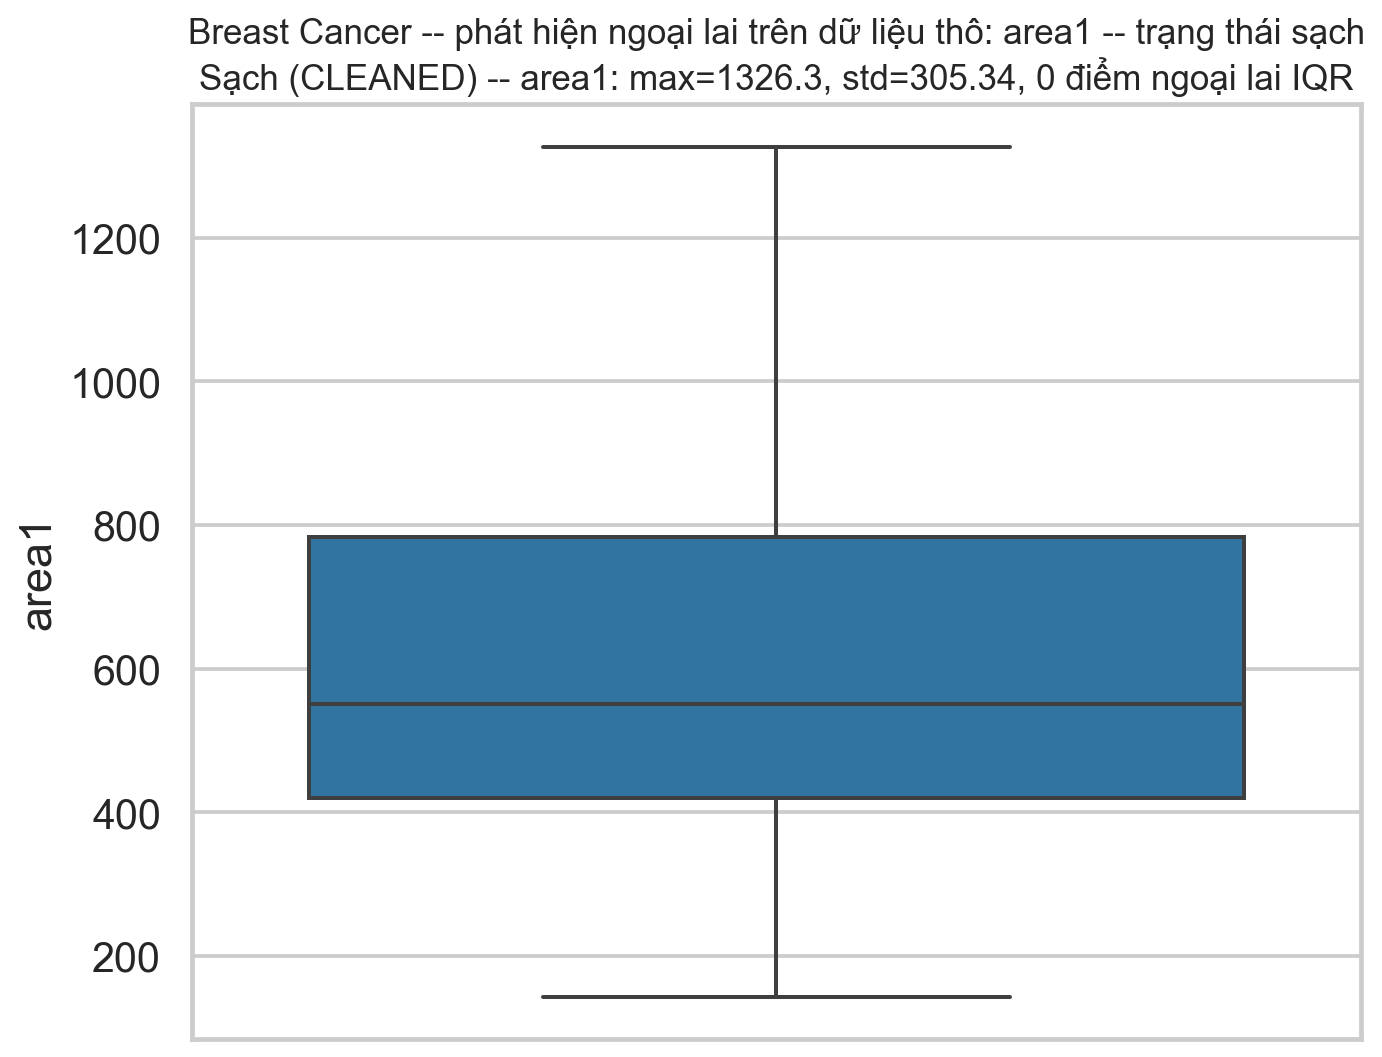
\includegraphics[width=0.72\textwidth]{images/ch3/breast_cancer_area1_boxplot_cleaned.png}
\captionsetup{justification=raggedright,singlelinecheck=false}
\caption[Boxplot \texttt{area1} sạch Breast Cancer]{Boxplot \texttt{area1} Breast Cancer ở \textbf{trạng thái sạch}: sau clipping IQR, các điểm ngoại lai được nén về ngưỡng trên hộp (max $\sim$2501 $\to$ $\sim$1326) nhưng vẫn giữ cấu trúc tách B/M.\\
\footnotesize Python source: \texttt{scripts/generate\_raw\_vs\_cleaned\_boxplots.py}.}
\label{fig:ch4_breast_cleaned_boxplot}
\end{figure}

\textbf{Bước 1. Phân loại bản chất biến.} Trước khi chọn thống kê và biểu đồ, các biến được phân loại theo bản chất đo lường. Với Breast Cancer, hầu hết đặc trưng đầu vào là Quantitative Continuous; riêng \texttt{Diagnosis} là biến Qualitative binary dùng để so sánh phân phối theo nhóm chẩn đoán.

\begin{table}[H]
\centering
\caption{Bước 1 -- Phân loại biến tiêu biểu trong Breast Cancer}
\label{tab:ch4_breast_variable_types}
\small
\begin{tabularx}{\textwidth}{p{0.18\textwidth}p{0.27\textwidth}p{0.25\textwidth}Y}
\toprule
Biến & Bản chất & Thống kê dùng & Biểu đồ phù hợp \\
\midrule
\texttt{Diagnosis} & Qualitative binary & Tần suất, mode & Bar chart \\
\texttt{radius1} & Quantitative Continuous & Mean, median, IQR & Histogram, boxplot \\
\texttt{texture1} & Quantitative Continuous & Mean, std, range & Histogram \\
\texttt{perimeter1} & Quantitative Continuous & Mean, median, IQR & Histogram, heatmap \\
\texttt{area1} & Quantitative Continuous & Range, variance, CV & Histogram, boxplot \\
\texttt{smoothness1} & Quantitative Continuous & Mean, median, IQR & Histogram, boxplot \\
\texttt{concavity1} & Quantitative Continuous & CV, skewness proxy & Histogram, boxplot \\
\bottomrule
\end{tabularx}
\end{table}

\textbf{Bước 2. Bảng tần suất và thống kê mô tả.} Biến \texttt{Diagnosis} được mô tả bằng tần suất tuyệt đối, tần suất tương đối và mode. Các biến hình thái định lượng được mô tả bằng mean, median, mode, percentile, range, variance, standard deviation, CV và IQR.

\begin{table}[H]
\centering
\caption[Bảng tần suất \texttt{Diagnosis} trong Breast Cancer]{Bước 2 -- Bảng tần suất biến \texttt{Diagnosis} trong Breast Cancer. Source: \texttt{outputs/tables/breast\_cancer\_frequency\_Diagnosis.csv}.}
\label{tab:ch4_breast_frequency}
\small
\begin{tabular}{lrr}
\toprule
\texttt{Diagnosis} & Tần suất tuyệt đối & Tần suất tương đối \\
\midrule
B (lành tính) & 357 & 62.74\% \\
M (ác tính) & 212 & 37.26\% \\
\bottomrule
\end{tabular}
\end{table}

\begin{table}[H]
\centering
\caption[Thống kê mô tả Breast Cancer]{Thống kê mô tả Breast Cancer: xu hướng trung tâm và độ phân tán. Source: \texttt{outputs/tables/breast\_cancer\_summary.csv}.}
\label{tab:ch4_breast_stats}
\scriptsize
\setlength{\tabcolsep}{3pt}
\begin{tabular}{lrrrrrrrrrr}
\toprule
Biến & Mean & Med & Mode & P25 & P75 & Range & Var & Std & CV & IQR \\
\midrule
\texttt{radius1} & 14.13 & 13.37 & 12.34 & 11.70 & 15.78 & 21.13 & 12.42 & 3.52 & 0.249 & 4.08 \\
\texttt{texture1} & 19.29 & 18.84 & 14.93 & 16.17 & 21.80 & 29.57 & 18.50 & 4.30 & 0.223 & 5.63 \\
\texttt{perimeter1} & 91.97 & 86.24 & 82.61 & 75.17 & 104.10 & 144.71 & 590.44 & 24.30 & 0.264 & 28.93 \\
\texttt{area1} & 654.89 & 551.10 & 512.20 & 420.30 & 782.70 & 2357.50 & 123843.6 & 351.91 & 0.537 & 362.40 \\
\texttt{smoothness1} & 0.096 & 0.096 & 0.101 & 0.086 & 0.105 & 0.111 & 0.0002 & 0.014 & 0.146 & 0.019 \\
\texttt{concavity1} & 0.089 & 0.062 & 0.000 & 0.030 & 0.131 & 0.427 & 0.006 & 0.080 & 0.898 & 0.101 \\
\bottomrule
\end{tabular}
\end{table}

\begin{table}[H]
\centering
\caption[Thống kê thô/sạch Breast Cancer]{So sánh thống kê mô tả Breast Cancer ở hai trạng thái: \textbf{thô} và \textbf{sạch} (clipping IQR trên 6 biến hình thái). Source: \texttt{outputs/tables/breast\_cancer\_summary.csv}.}
\label{tab:ch4_breast_stats_raw_clean}
\footnotesize
\setlength{\tabcolsep}{4pt}
\begin{tabular}{lcrrrrrr}
\toprule
Biến & Trạng thái & Mean & Median & Std & \textbf{Max} & \textbf{Range} & IQR \\
\midrule
\texttt{radius1} & thô & 14.13 & 13.37 & 3.52 & \textbf{28.11} & 21.13 & 4.08 \\
 & sạch & 14.06 & 13.37 & 3.34 & \textbf{21.90} & 14.92 & 4.08 \\
\midrule
\texttt{texture1} & thô & 19.29 & 18.84 & 4.30 & 39.28 & 29.57 & 5.63 \\
 & sạch & 19.25 & 18.84 & 4.19 & 30.24 & 20.54 & 5.63 \\
\midrule
\texttt{perimeter1} & thô & 91.97 & 86.24 & 24.30 & 188.50 & 144.71 & 28.93 \\
 & sạch & 91.54 & 86.24 & 23.05 & 147.50 & 103.70 & 28.93 \\
\midrule
\texttt{area1} & thô & 654.89 & 551.10 & 351.91 & \textbf{2501.00} & 2357.50 & 362.40 \\
 & sạch & 639.77 & 551.10 & 305.34 & \textbf{1326.30} & 1182.80 & 362.40 \\
\midrule
\texttt{smoothness1} & thô & 0.096 & 0.096 & 0.014 & 0.163 & 0.111 & 0.019 \\
 & sạch & 0.096 & 0.096 & 0.014 & 0.134 & 0.076 & 0.019 \\
\midrule
\texttt{concavity1} & thô & 0.089 & 0.062 & 0.080 & 0.427 & 0.427 & 0.101 \\
 & sạch & 0.087 & 0.062 & 0.074 & 0.282 & 0.282 & 0.101 \\
\bottomrule
\end{tabular}
\end{table}

\textit{Nhận xét thô/sạch.} \texttt{area1} là biến có thang đo lớn nhất và cũng giảm max mạnh nhất sau clipping: từ 2501 xuống 1326, đồng thời standard deviation giảm từ 351.91 xuống 305.34. \texttt{radius1} giảm max từ 28.11 xuống 21.90. Đáng chú ý, median và IQR của các biến đều không đổi, cho thấy clipping chỉ nén phần đuôi mà không dịch chuyển vùng trung tâm của phân phối. Đây là điều quan trọng vì tín hiệu phân biệt khối u lành/ác chủ yếu nằm ở sự tách biệt trung tâm và khoảng tứ phân vị giữa hai nhóm.

\textbf{Bước 3. Trực quan hóa dữ liệu.} Hệ thống biểu đồ được lựa chọn theo cùng cấu trúc với Heart Disease: bar chart cho phân bố \texttt{Diagnosis}, histogram cho \texttt{radius1}, boxplot theo target để đọc khả năng phân tách B/M, scatter plot cho quan hệ hai đặc trưng, đối chiếu thô/sạch để đánh giá clipping và heatmap để khảo sát tương quan giữa các biến hình thái.

\begin{figure}[H]
\centering
\begin{subfigure}{0.90\textwidth}
 \centering
 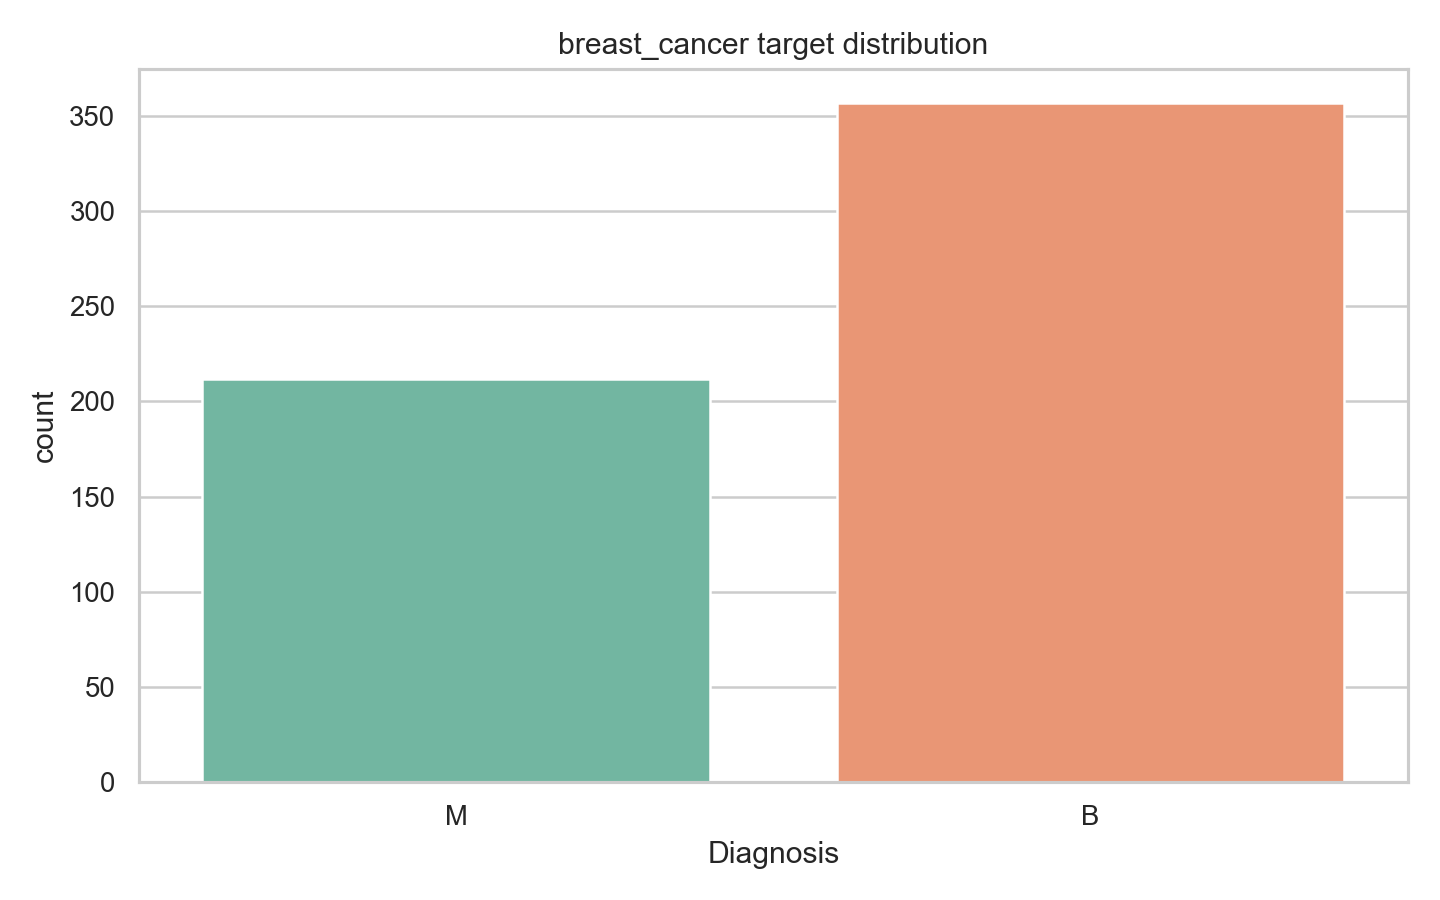
\includegraphics[width=\textwidth]{images/ch3/breast_cancer_target_distribution.png}
 \caption{Python -- Phân bố \texttt{Diagnosis}}
\end{subfigure}
\par\medskip
\begin{subfigure}{0.90\textwidth}
 \centering
 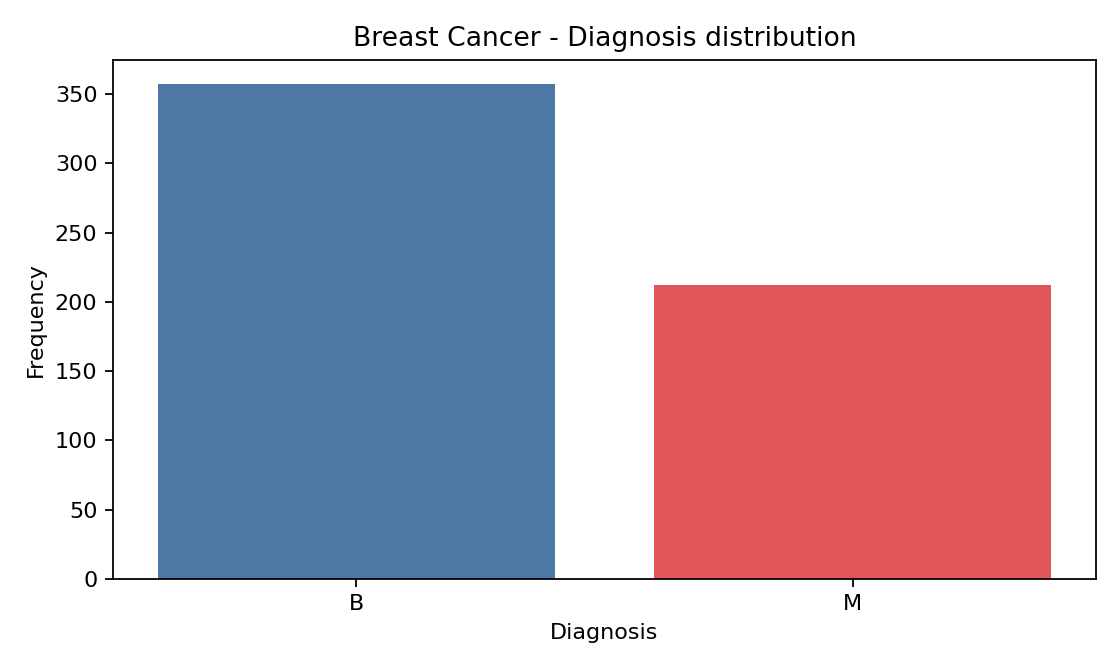
\includegraphics[width=\textwidth]{images/ch3/excel_breast_target_distribution_preview.png}
 \caption{Excel -- Phân bố \texttt{Diagnosis}}
\end{subfigure}
\captionsetup{justification=raggedright,singlelinecheck=false}
\caption[Phân bố target Breast Cancer: Python và Excel]{Phân bố \texttt{Diagnosis} trong Breast Cancer, đối chiếu giữa Python và Excel.\\
\footnotesize Python source: \texttt{src/analyze\_tabular\_health.py}.\\
Excel source/workbook: \texttt{src/create\_excel\_visualizations.py}, \texttt{excel/excel\_visualization\_comparison\_native.xlsx}, sheet \texttt{Breast Target}.}
\label{fig:ch4_breast_target}
\end{figure}

\textbf{Nhận xét Hình \ref{fig:ch4_breast_target}.} Lớp B chiếm 62.74\%, lớp M chiếm 37.26\%; dữ liệu không cân bằng nhẹ nhưng không quá cực đoan.

\begin{figure}[H]
\centering
\begin{subfigure}{0.90\textwidth}
 \centering
 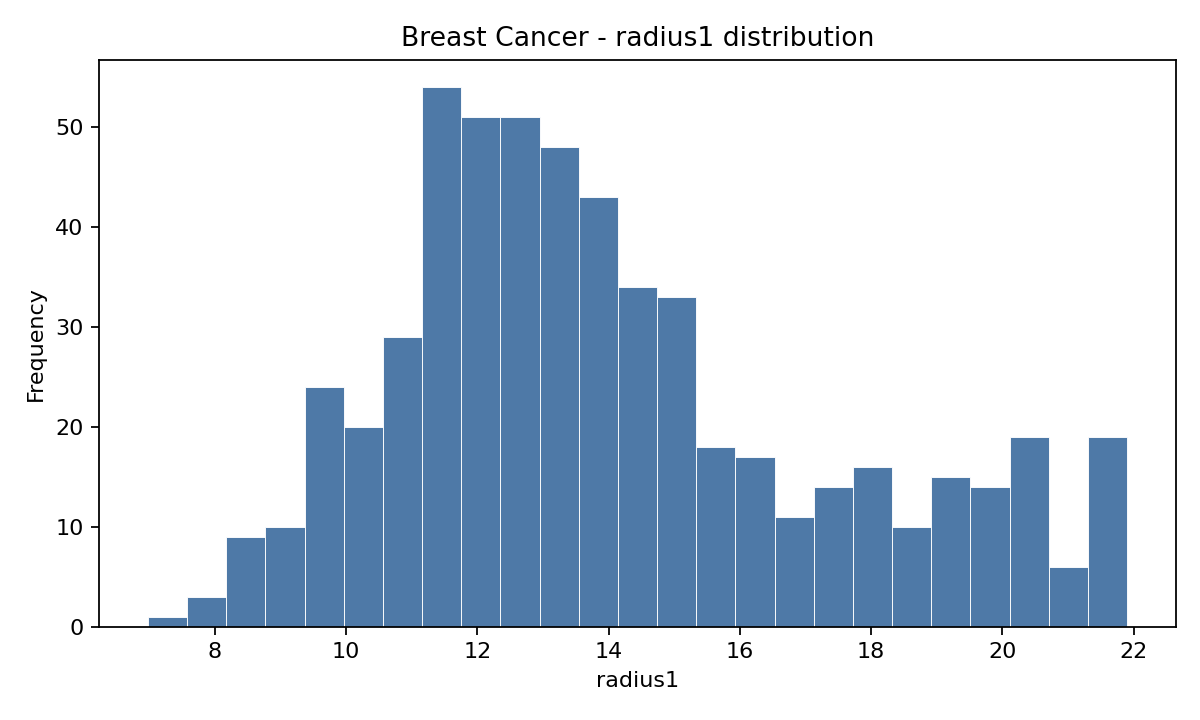
\includegraphics[width=\textwidth]{images/ch3/breast_cancer_radius1_hist.png}
 \caption{Python -- Histogram \texttt{radius1}}
\end{subfigure}
\par\medskip
\begin{subfigure}{0.90\textwidth}
 \centering
 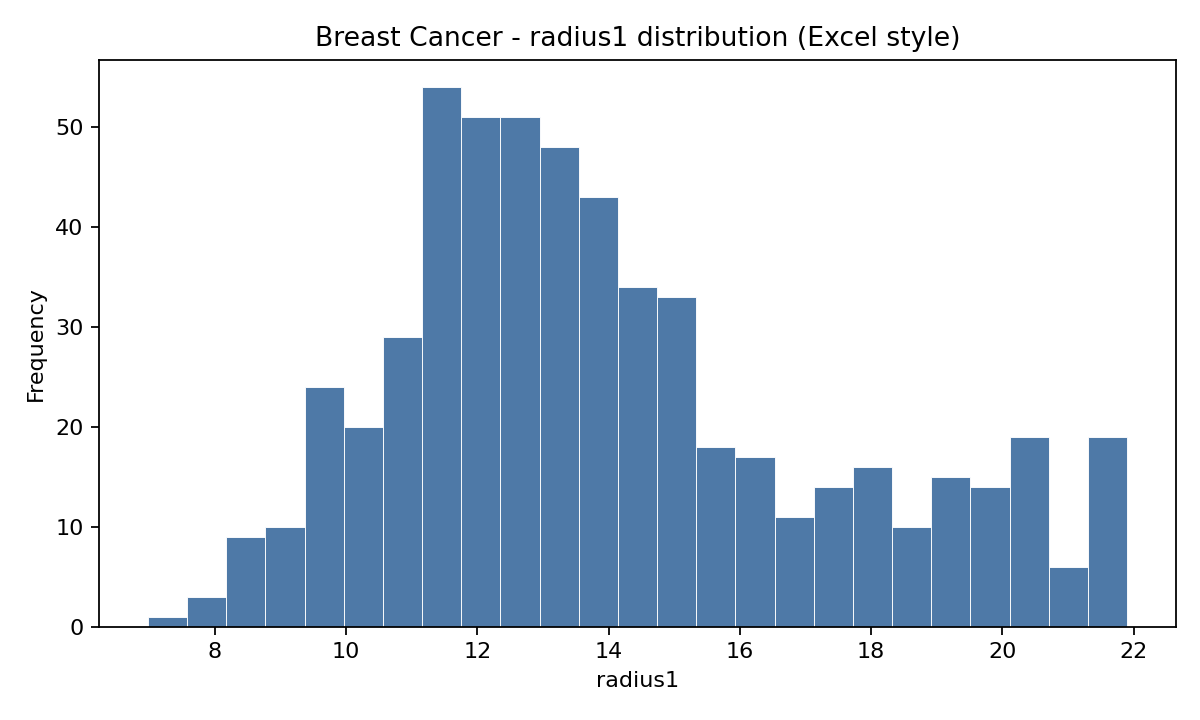
\includegraphics[width=\textwidth]{images/ch3/excel_breast_radius_hist_preview.png}
 \caption{Excel -- Histogram \texttt{radius1}}
\end{subfigure}
\captionsetup{justification=raggedright,singlelinecheck=false}
\caption[Histogram \texttt{radius1} Breast Cancer: Python và Excel]{Phân phối \texttt{radius1} trong Breast Cancer, đối chiếu giữa Python và Excel.\\
\footnotesize Python source: \texttt{src/analyze\_tabular\_health.py}.\\
Excel source/workbook: \texttt{src/create\_excel\_visualizations.py}, \texttt{excel/excel\_visualization\_comparison\_native.xlsx}, sheet \texttt{Breast Radius Hist}.}
\label{fig:ch4_breast_radius_hist}
\end{figure}

\textbf{Nhận xét Hình \ref{fig:ch4_breast_radius_hist}.} \texttt{radius1} lệch phải nhẹ: mean 14.13 lớn hơn median 13.37.

\begin{figure}[H]
\centering
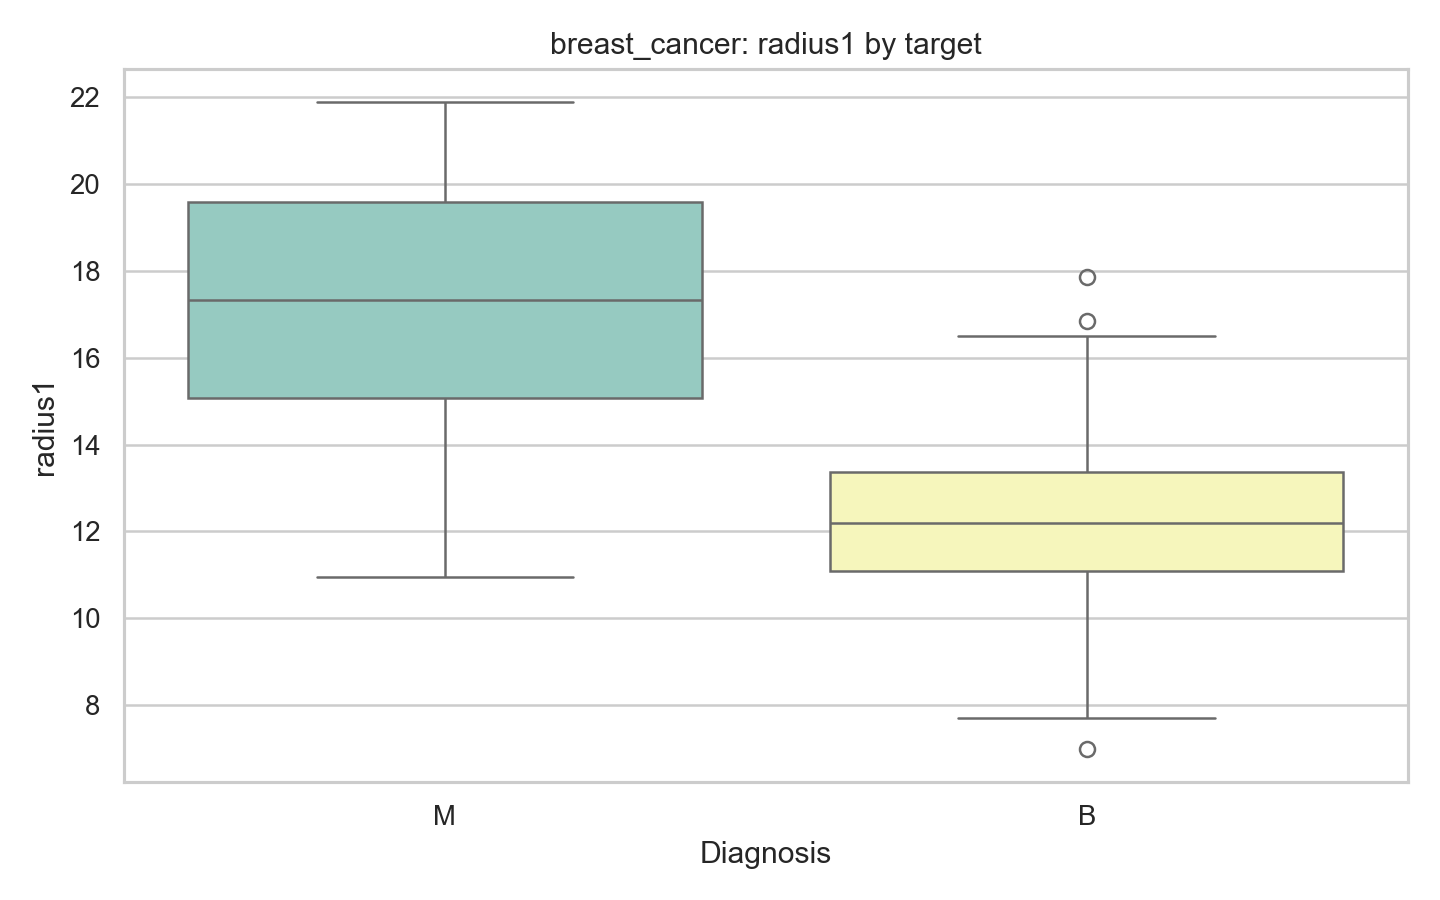
\includegraphics[width=0.90\textwidth]{images/ch3/breast_cancer_radius1_boxplot_by_target.png}
\captionsetup{justification=raggedright,singlelinecheck=false}
\caption[Boxplot \texttt{radius1} Breast Cancer]{Boxplot \texttt{radius1} theo chẩn đoán B/M.\\
\footnotesize Python source: \texttt{src/analyze\_tabular\_health.py}.}
\label{fig:ch4_breast_radius_boxplot}
\end{figure}

\textbf{Nhận xét Hình \ref{fig:ch4_breast_radius_boxplot}.} Nhóm ác tính (M) có trung vị và khoảng phân vị \texttt{radius1} cao hơn nhóm lành tính (B), hai hộp tách khá rõ.

\begin{figure}[H]
\centering
\begin{subfigure}{0.90\textwidth}
 \centering
 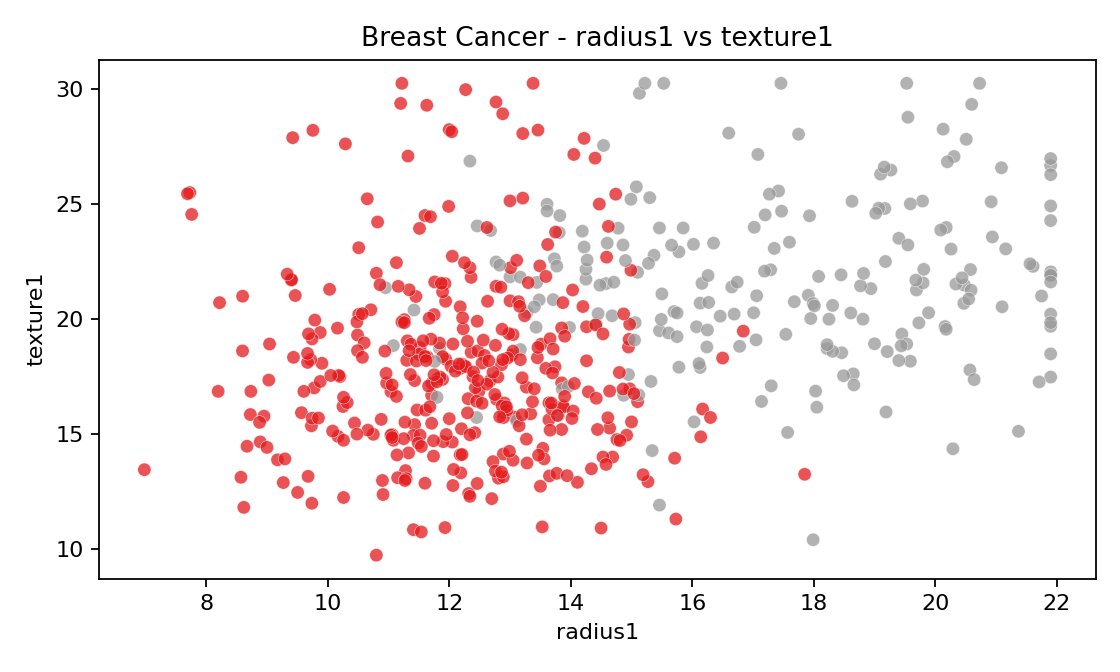
\includegraphics[width=\textwidth]{images/ch3/breast_cancer_radius_texture_scatter.png}
 \caption{Python -- Scatter \texttt{radius1}--\texttt{texture1}}
\end{subfigure}
\par\medskip
\begin{subfigure}{0.90\textwidth}
 \centering
 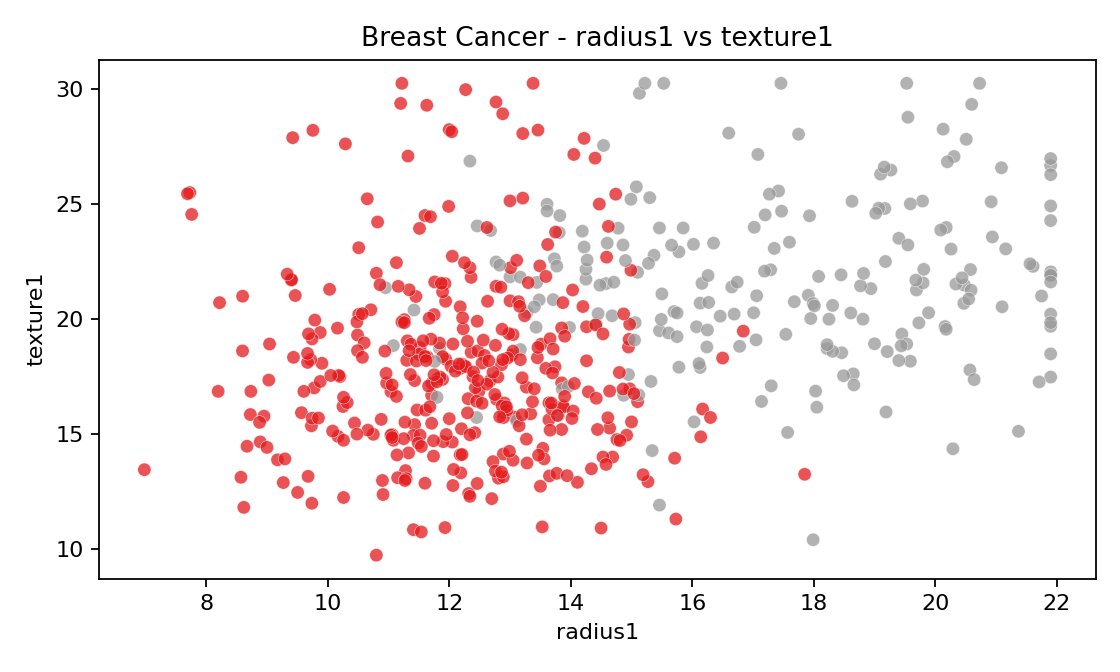
\includegraphics[width=\textwidth]{images/ch3/excel_breast_radius_texture_scatter_preview.png}
 \caption{Excel -- Scatter \texttt{radius1}--\texttt{texture1}}
\end{subfigure}
\captionsetup{justification=raggedright,singlelinecheck=false}
\caption[Scatter Breast Cancer: Python và Excel]{Scatter giữa \texttt{radius1} và \texttt{texture1}, đối chiếu giữa Python và Excel.\\
\footnotesize Python source: \texttt{src/analyze\_tabular\_health.py}.\\
Excel source/workbook: \texttt{src/create\_excel\_visualizations.py}, \texttt{excel/excel\_visualization\_comparison\_native.xlsx}, sheet \texttt{Breast Scatter}.}
\label{fig:ch4_breast_scatter}
\end{figure}

\textbf{Nhận xét Hình \ref{fig:ch4_breast_scatter}.} Nhóm M thường dịch về vùng \texttt{radius1} lớn hơn, còn \texttt{texture1} bổ sung độ tách theo chiều thứ hai.

\textit{Đối chiếu thô/sạch.} Ba biểu đồ tiếp theo đặt dữ liệu thô (đỏ) cạnh dữ liệu sạch (xanh), qua đó thể hiện trực quan tác động của clipping IQR trên các biến hình thái.

\begin{figure}[H]
\centering
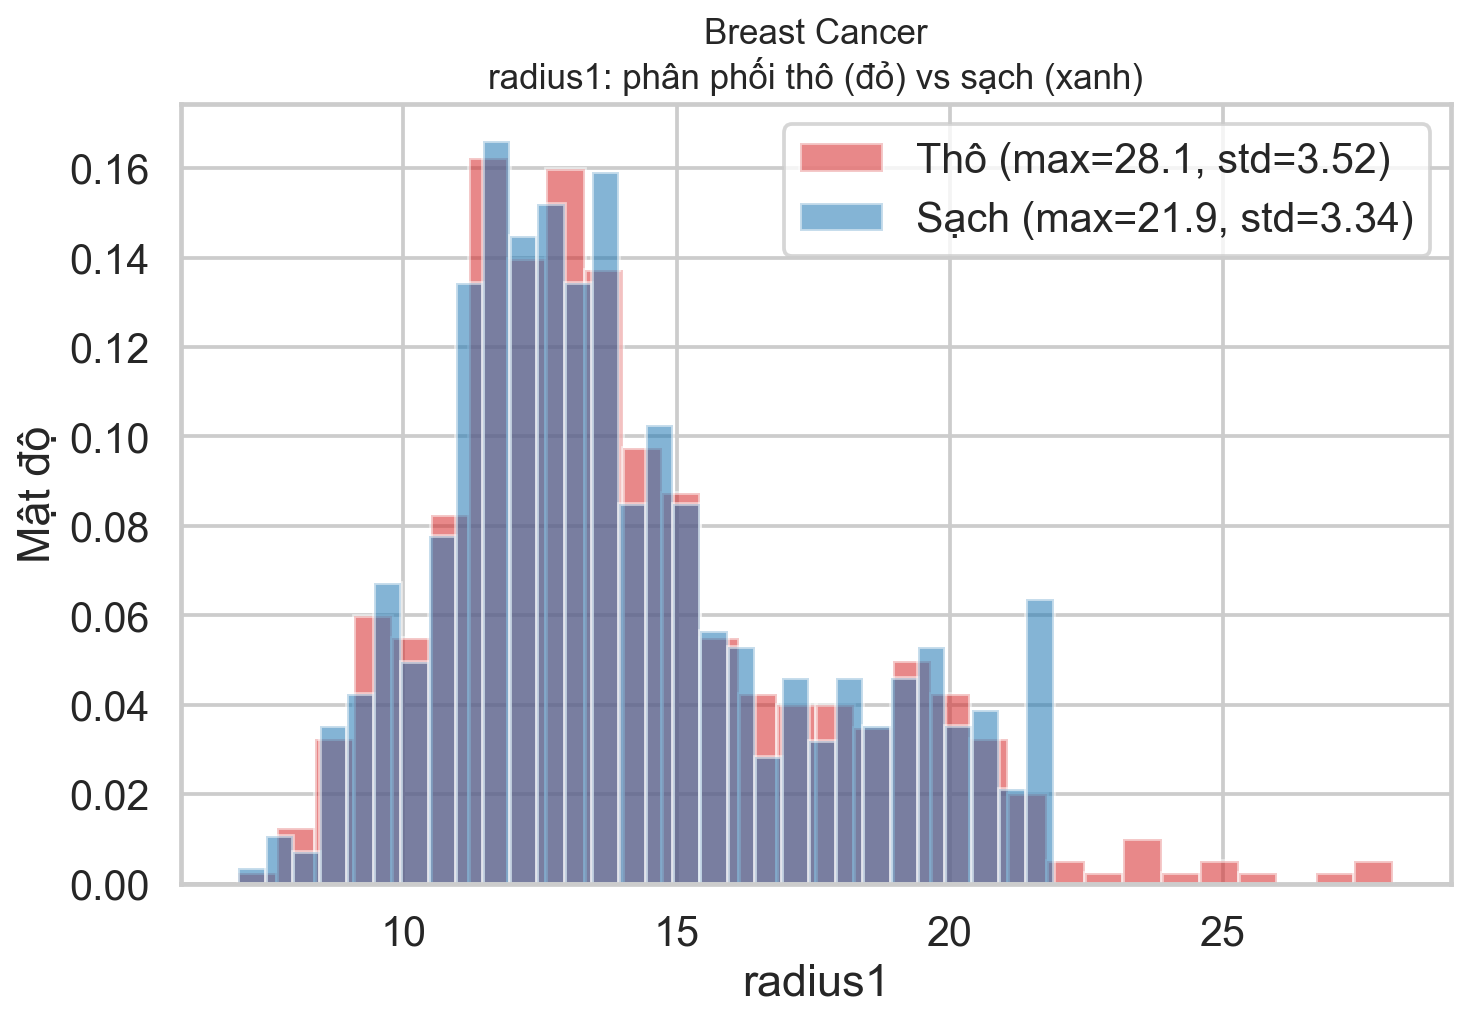
\includegraphics[width=0.82\textwidth]{images/ch3/breast_cancer_radius1_hist_raw_vs_cleaned.png}
\captionsetup{justification=raggedright,singlelinecheck=false}
\caption[Histogram \texttt{radius1} thô/sạch Breast Cancer]{Histogram \texttt{radius1} Breast Cancer: dữ liệu thô (đỏ, đuôi phải tới $\sim$28) chồng lên dữ liệu sạch (xanh, đuôi nén về $\sim$21.9).\\
\footnotesize Python source: \texttt{scripts/generate\_raw\_vs\_cleaned\_boxplots.py}.}
\label{fig:ch4_breast_hist_compare}
\end{figure}

\begin{figure}[H]
\centering
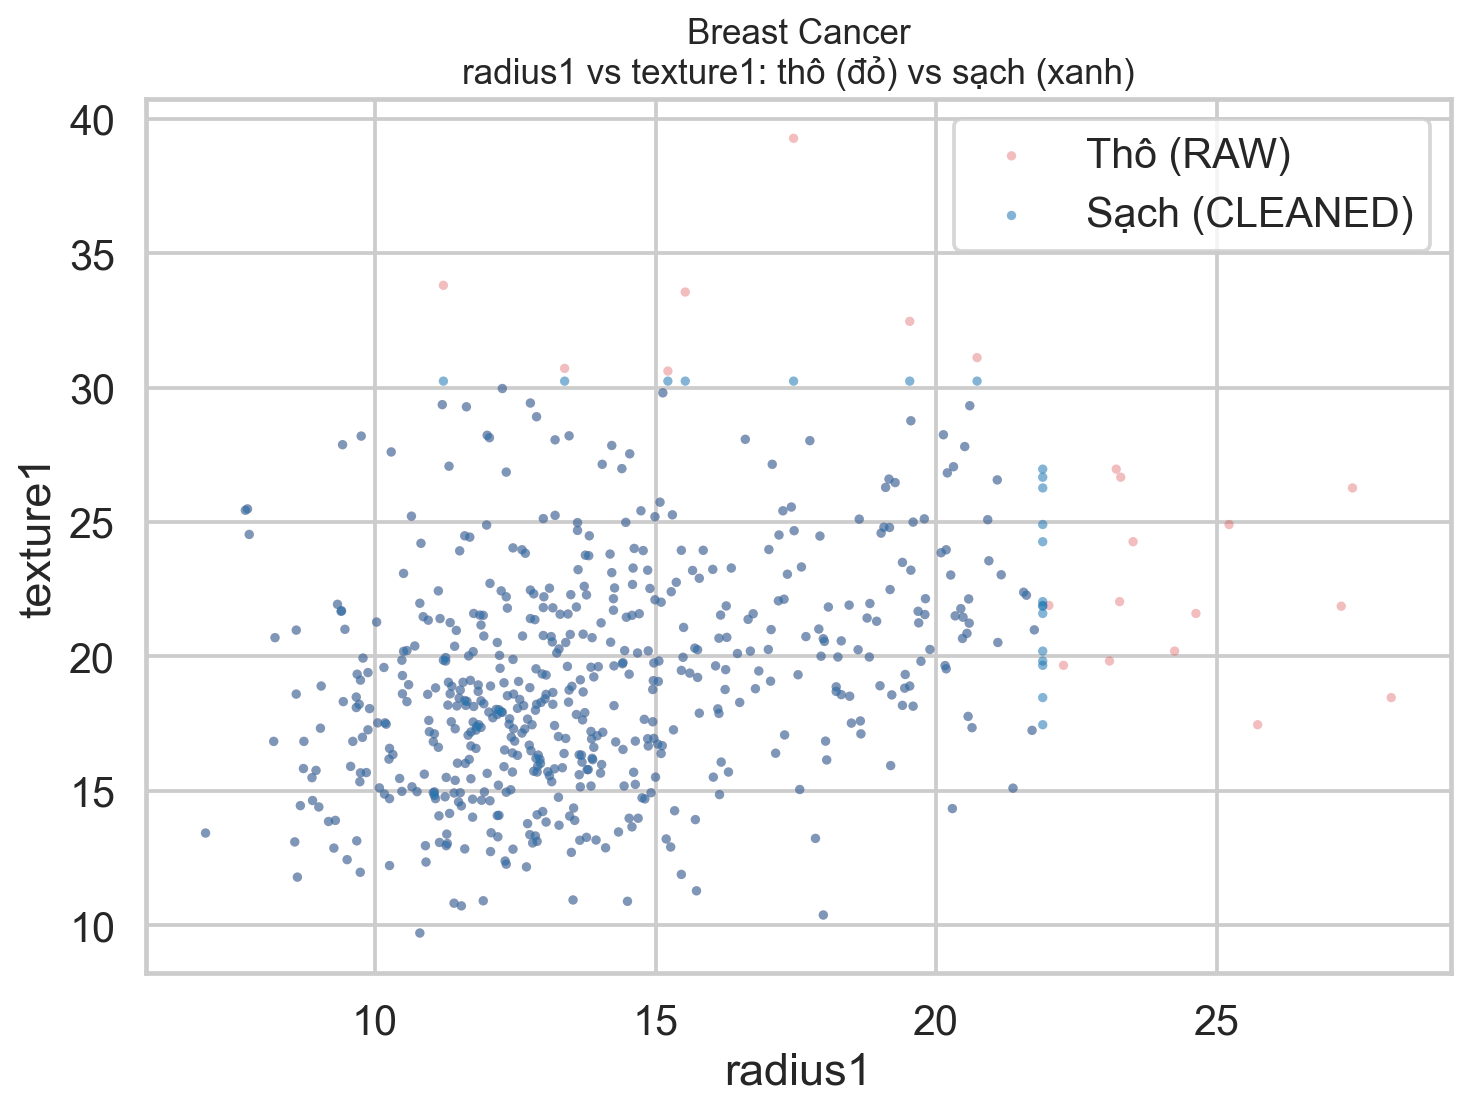
\includegraphics[width=0.82\textwidth]{images/ch3/breast_cancer_radius_texture_scatter_raw_vs_cleaned.png}
\captionsetup{justification=raggedright,singlelinecheck=false}
\caption[Scatter \texttt{radius1}--\texttt{texture1} thô/sạch Breast Cancer]{Scatter \texttt{radius1}--\texttt{texture1} Breast Cancer: dữ liệu thô (đỏ, mờ) phủ tới radius1$\sim$28; dữ liệu sạch (xanh) bị nén nhưng vùng M (bên phải) vẫn tách rõ.\\
\footnotesize Python source: \texttt{scripts/generate\_raw\_vs\_cleaned\_boxplots.py}.}
\label{fig:ch4_breast_scatter_compare}
\end{figure}

\begin{figure}[H]
\centering
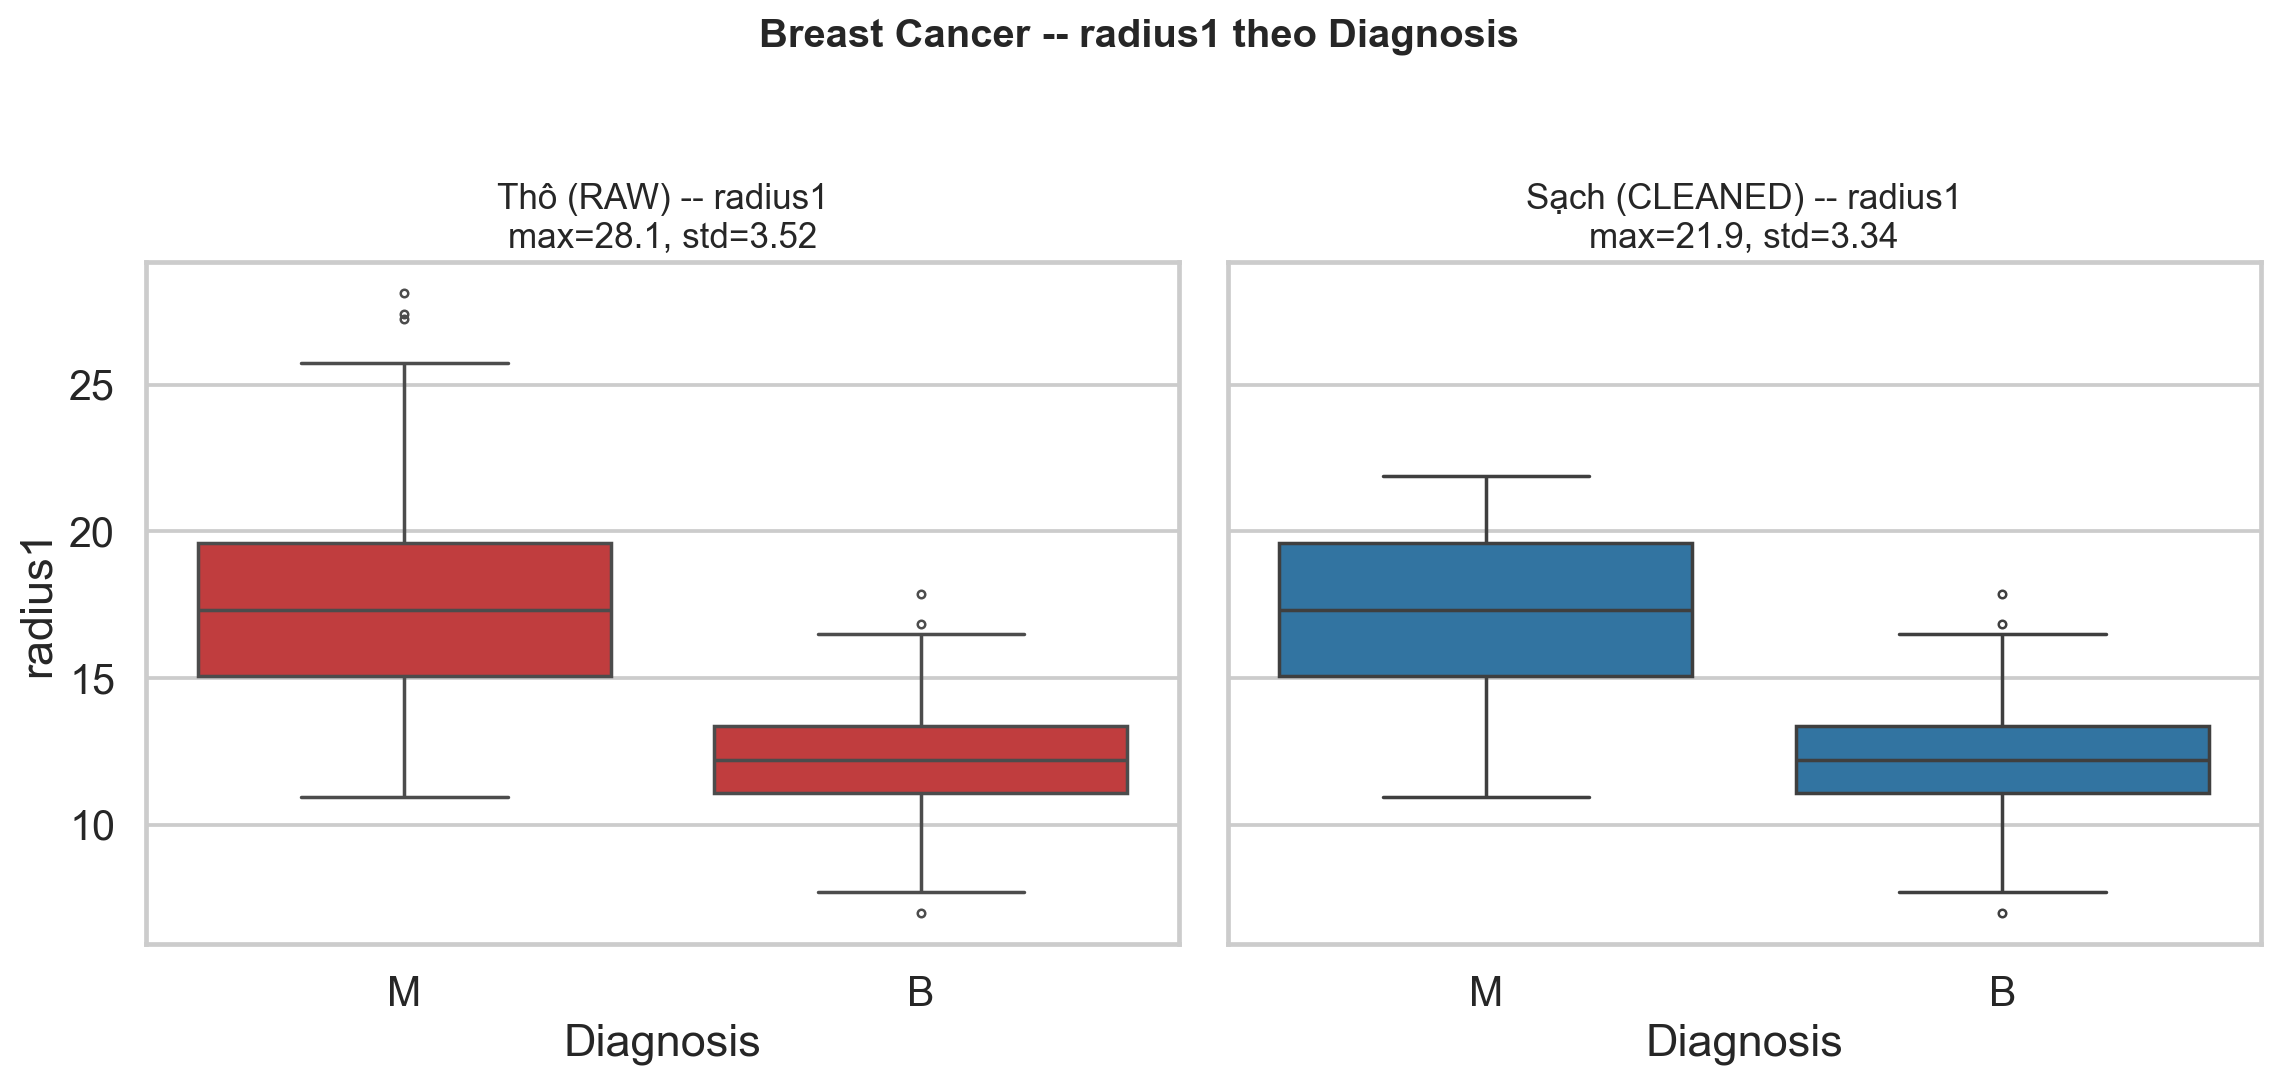
\includegraphics[width=0.95\textwidth]{images/ch3/breast_cancer_radius1_boxplot_by_target_raw_vs_cleaned.png}
\captionsetup{justification=raggedright,singlelinecheck=false}
\caption[Boxplot \texttt{radius1} theo Diagnosis thô/sạch Breast Cancer]{Boxplot \texttt{radius1} theo \texttt{Diagnosis}: thô (trái) có nhiều điểm ngoại lai; sạch (phải) giảm ngoại lai nhưng trung vị nhóm M vẫn cao hơn B rõ rệt.\\
\footnotesize Python source: \texttt{scripts/generate\_raw\_vs\_cleaned\_boxplots.py}.}
\label{fig:ch4_breast_boxplot_by_target_compare}
\end{figure}

\textbf{Nhận xét.} Histogram \texttt{radius1} (Hình~\ref{fig:ch4_breast_hist_compare}) cho thấy đuôi phải dữ liệu thô tới $\sim$28 bị nén về $\sim$21.9 ở dữ liệu sạch, phần lõi vẫn trùng nhau. Scatter (Hình~\ref{fig:ch4_breast_scatter_compare}) xác nhận vùng cao của \texttt{radius1} (đỏ) bị cắt nhưng cụm nhóm M (bên phải) vẫn giữ vị trí tương đối. Boxplot theo Diagnosis (Hình~\ref{fig:ch4_breast_boxplot_by_target_compare}) cho thấy sau clipping số điểm ngoài râu giảm, nhưng hai hộp B/M vẫn tách rõ -- clipping giảm nhiễu mà không phá tín hiệu chẩn đoán.

\begin{figure}[H]
\centering
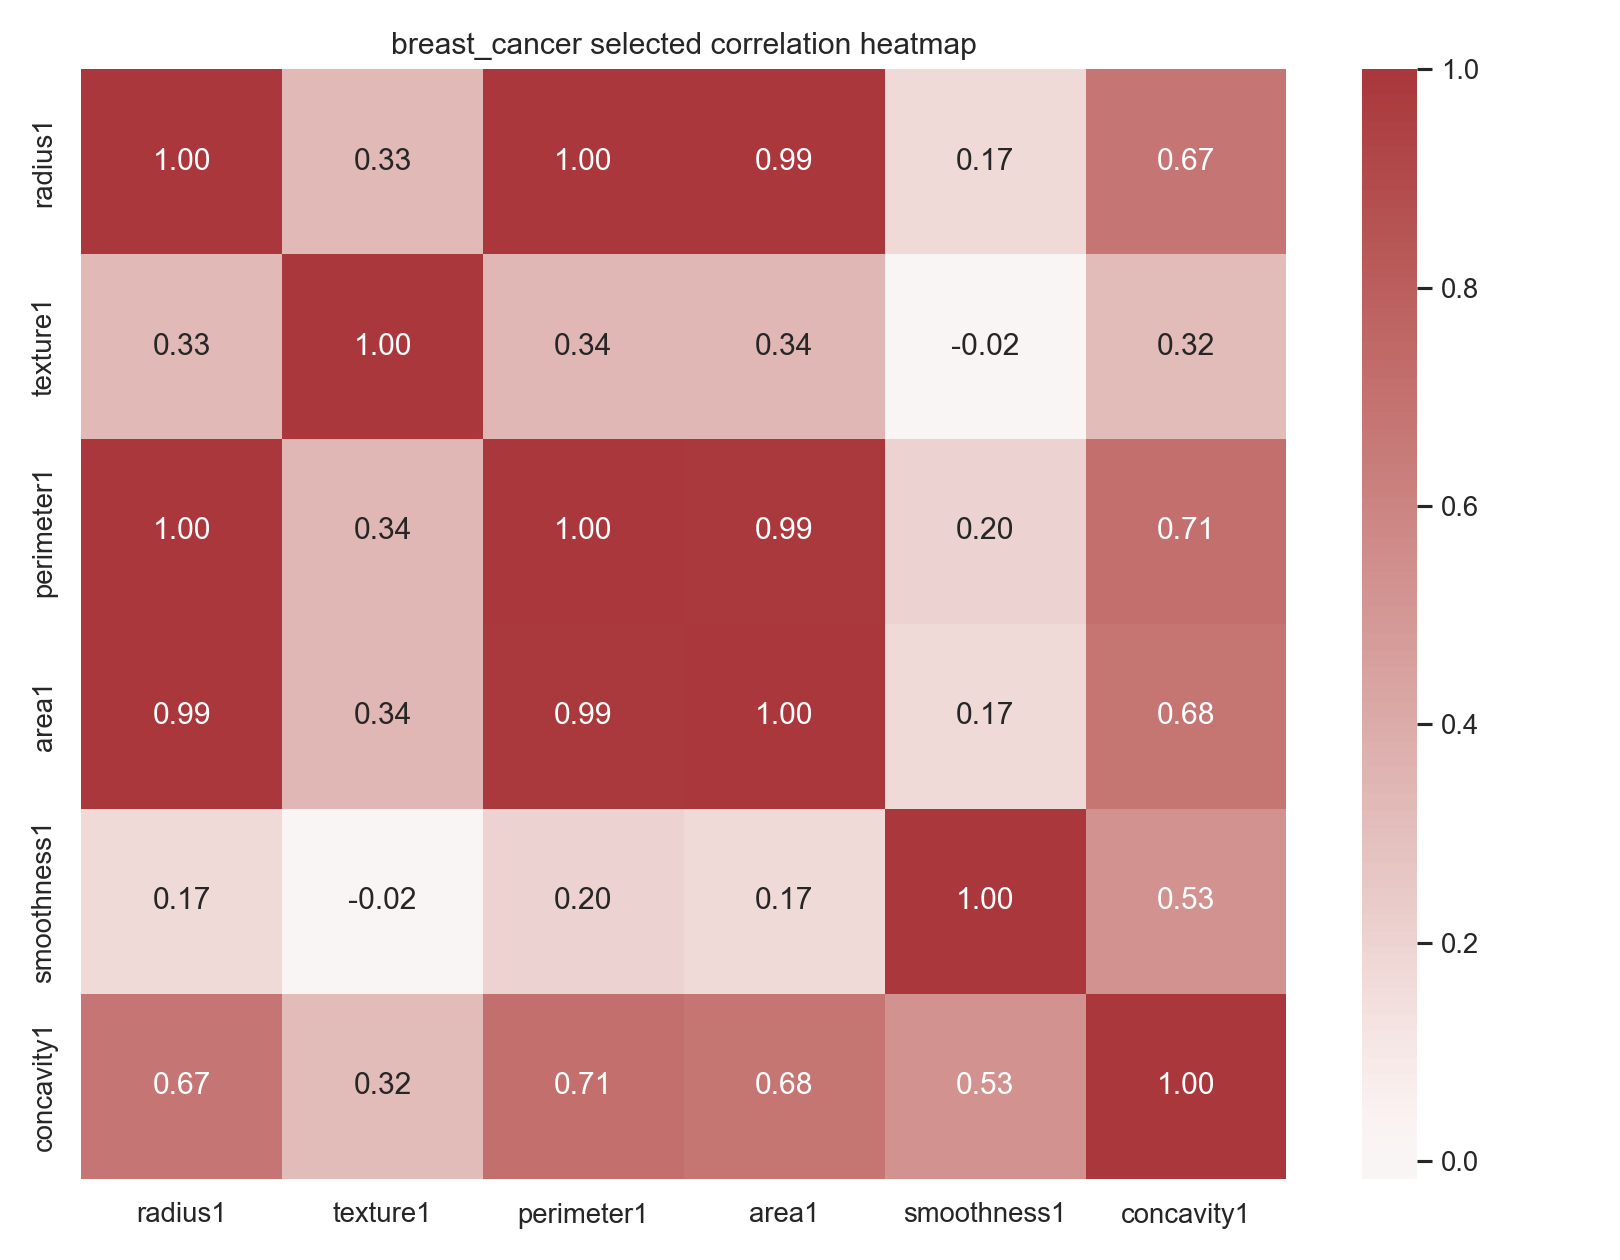
\includegraphics[width=0.86\textwidth]{images/ch3/breast_cancer_correlation_heatmap.png}
\captionsetup{justification=raggedright,singlelinecheck=false}
\caption[Heatmap tương quan Breast Cancer]{Heatmap tương quan các đặc trưng hình thái Breast Cancer.\\
\footnotesize Python source: \texttt{src/analyze\_tabular\_health.py}.}
\label{fig:ch4_breast_corr}
\end{figure}

\textbf{Nhận xét Hình \ref{fig:ch4_breast_corr}.} Nhóm biến kích thước như \texttt{radius1}, \texttt{perimeter1} và \texttt{area1} tương quan rất mạnh, phản ánh chúng cùng đo quy mô khối u từ các góc nhìn khác nhau. Khi đưa vào mô hình tuyến tính, cần chú ý đa cộng tuyến; với các mô hình cây, nhóm biến này vẫn có thể hỗ trợ phân tách lớp hiệu quả.

\textbf{Nhận xét về hình dáng phân phối.} Các biến kích thước khối u như \texttt{radius1}, \texttt{perimeter1} và \texttt{area1} đều có mean lớn hơn median, cho thấy phân phối lệch phải. Điều này phù hợp với thực tế dữ liệu: phần lớn khối u tập trung ở kích thước trung bình hoặc nhỏ, trong khi một số ca ác tính có kích thước lớn tạo đuôi phải. \texttt{concavity1} lệch phải mạnh hơn, với mode bằng 0, phản ánh nhiều quan sát có độ lõm thấp nhưng vẫn tồn tại một nhóm nhỏ có độ lõm cao.

\textbf{Bước 4. So sánh trước--sau tiền xử lý.} Bảng~\ref{tab:ch4_breast_stats_raw_clean} đặt các chỉ số của trạng thái thô cạnh trạng thái sạch; các hình thô/sạch ở trên minh họa trực tiếp tác động của clipping IQR.

Bảng~\ref{tab:ch4_breast_stats_raw_clean} cho thấy sự khác biệt giữa thô và sạch hoàn toàn đến từ xử lý ngoại lai, vì bộ dữ liệu không có ô khuyết. Trên dữ liệu thô, \texttt{radius1} có các ca cực trị vượt 25 và \texttt{area1} có range xấp xỉ 2357; sau clipping IQR, các đỉnh này được nén về biên hộp, làm standard deviation và range giảm. Tuy nhiên, trung vị và IQR vẫn ổn định, đồng thời boxplot theo chẩn đoán (Hình~\ref{fig:ch4_breast_boxplot_by_target_compare}) cho thấy nhóm M vẫn có trung vị \texttt{radius1} cao hơn nhóm B. Như vậy, tiền xử lý làm giảm ảnh hưởng của cực trị nhưng không làm mất tín hiệu phân loại chẩn đoán.

\textbf{Kết luận cho Breast Cancer.} Có ba kết quả chính rút ra từ phân tích. Thứ nhất, dữ liệu không có ô khuyết, nên bước chuẩn bị tập trung vào kiểm soát ngoại lai và giữ đơn vị đo gốc để diễn giải hình thái khối u. Thứ hai, clipping IQR làm giảm đuôi phải của các biến kích thước, đặc biệt \texttt{area1} và \texttt{radius1}, nhưng không làm thay đổi median/IQR. Thứ ba, tín hiệu phân biệt giữa B và M vẫn rõ sau tiền xử lý, thể hiện qua boxplot và scatter plot; vì vậy dữ liệu sạch phù hợp hơn cho mô hình học máy mà vẫn bảo toàn ý nghĩa lâm sàng.


\subsection{Nhóm B: dữ liệu chuỗi thời gian và cảm biến}

Nhóm B nhấn mạnh thứ tự thời gian và tín hiệu cảm biến. Khác với dữ liệu bảng ở Nhóm A, bước phân tích cần giữ trục thời gian, kiểm tra missing theo chuỗi, dùng line chart để đọc xu hướng/mùa vụ. Đặc thù của Nhóm B là áp dụng hai nhóm kỹ thuật xử lý chuỗi thời gian:

\begin{itemize}[leftmargin=*]
    \item \textbf{Điền khuyết chuỗi thời gian:} vì dữ liệu cảm biến thu thập theo chu kỳ cố định (10 phút với Appliances Energy, 50~Hz với MHEALTH), khi có ô NaN do lỗi cảm biến, phương pháp điền phải tôn trọng thứ tự thời gian: \emph{forward fill} (lấy giá trị quan sát trước), \emph{backward fill} (lấy giá trị quan sát sau) hoặc \emph{linear interpolation} (nội suy tuyến tính giữa hai điểm). Các phương pháp này phù hợp hơn mean/median vì chúng giữ được tính liên tục của tín hiệu vật lý.
    \item \textbf{Biến đổi chuỗi để ổn định:} \emph{log-transform} ($\log(1+x)$) nén các đỉnh lớn và làm phương sai ổn định hơn; \emph{differencing} (hiệu phân bậc một, $y_t' = y_t - y_{t-1}$) loại bỏ trend/mức nền, đưa chuỗi về dao động quanh 0 -- điều kiện quan trọng cho mô hình ARIMA và phân tích thay đổi ngắn hạn; \emph{rolling statistics} (trung bình trượt, độ lệch chuẩn trượt) làm rõ xu hướng nền và phát hiện thay đổi phương sai theo thời gian.
\end{itemize}

Trạng thái thô được dùng để nhận diện Null/NaN và các đoạn đứt gãy trên line chart; trạng thái sau xử lý áp dụng forward/backward fill hoặc linear interpolation cho khoảng trống, rồi log-transform/differencing/rolling để ổn định chuỗi. Cả hai trạng thái được so sánh song song để đánh giá chất lượng.

\subsubsection{Appliances Energy Prediction}

Appliances Energy có 19\,735 quan sát theo chu kỳ 10 phút. Năm chuỗi tiêu biểu gồm \texttt{Appliances}, \texttt{lights}, \texttt{T1}, \texttt{RH\_1}, \texttt{T\_out}; ngoài ra dùng \texttt{Appliances\_log1p}, \texttt{Appliances\_diff} và rolling statistics để đánh giá độ ổn định.

\textbf{Trạng thái dữ liệu thô (chưa làm sạch).} Ở trạng thái thô, Appliances Energy \emph{không có ô khuyết thiếu} (0/19\,735 dòng, theo \texttt{outputs/tables/appliances\_energy\_missing\_values.csv}).

\begin{figure}[H]
\centering
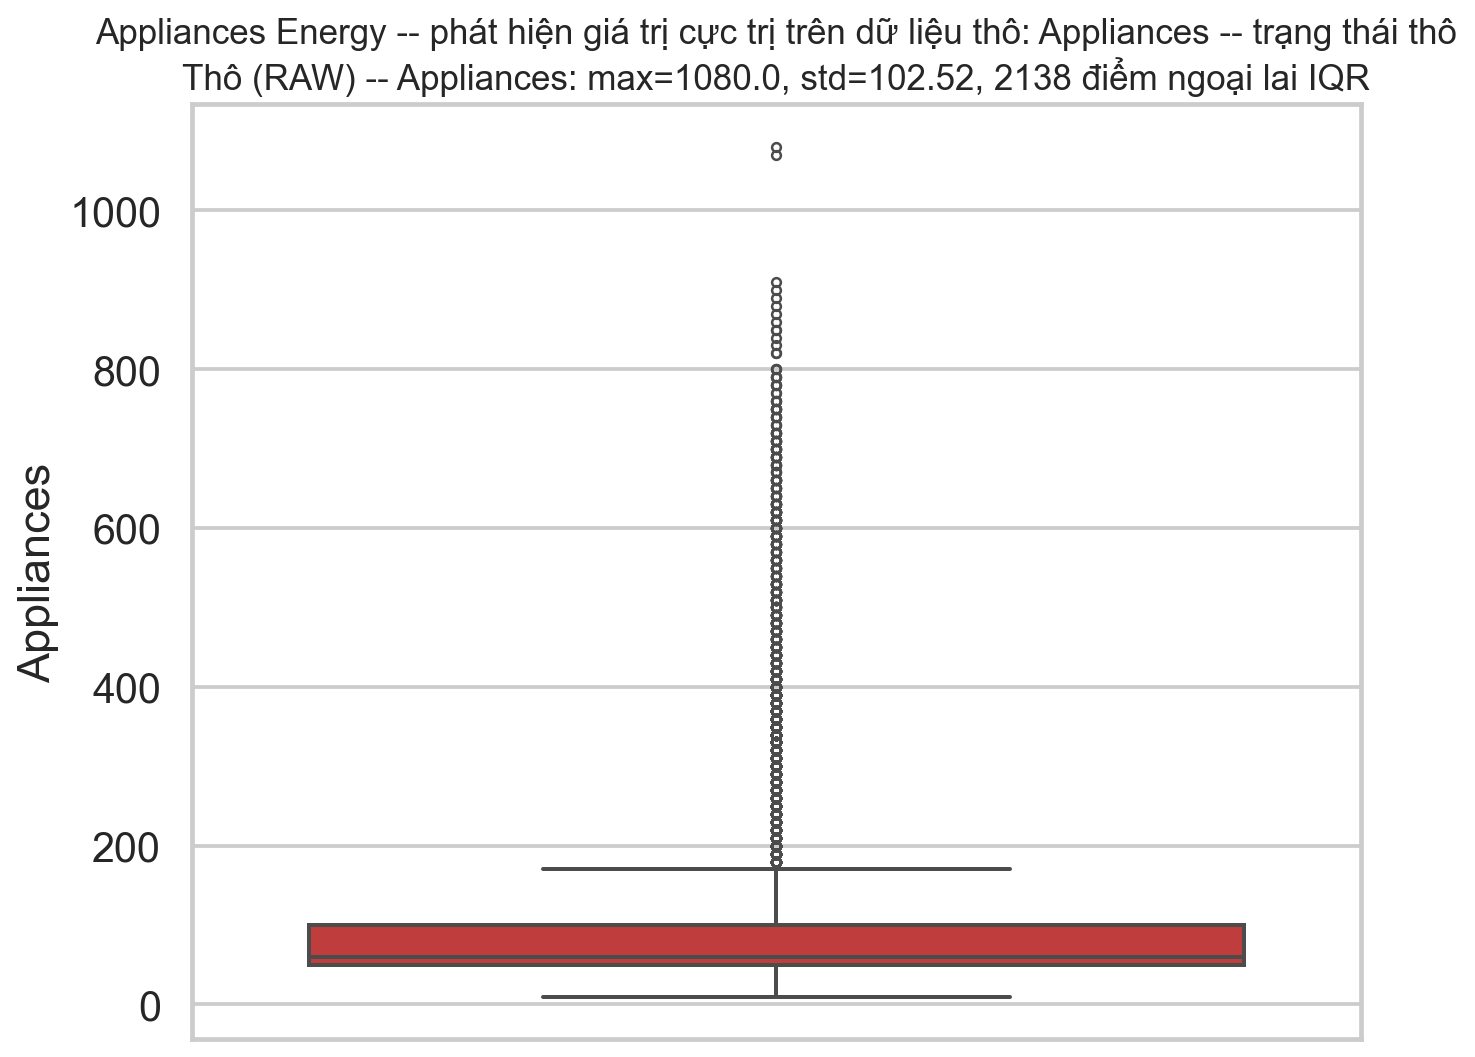
\includegraphics[width=0.72\textwidth]{images/ch3/appliances_energy_Appliances_boxplot_raw.png}
\captionsetup{justification=raggedright,singlelinecheck=false}
\caption[Boxplot \texttt{Appliances} thô]{Boxplot \texttt{Appliances} ở \textbf{trạng thái thô}: hàng nghìn điểm đỉnh tiêu thụ tới 1080 Wh (median 60). Đây là target dự báo nên sẽ \emph{không} clipping để bảo toàn giá trị thực.\\
\footnotesize Python source: \texttt{scripts/generate\_raw\_vs\_cleaned\_boxplots.py}.}
\label{fig:ch4_appliances_raw_boxplot}
\end{figure}

\textit{Phát hiện đoạn đứt/giá trị cực trị trên dữ liệu thô (line chart / boxplot).} Dưới boxplot trạng thái thô (Hình~\ref{fig:ch4_appliances_raw_boxplot}), vì chuỗi thực không có NaN nên line chart trạng thái thô (Hình~\ref{fig:ch4_appliances_daily_line}) \emph{không bị đứt gãy}; tuy nhiên, line chart và boxplot cho thấy: (a) biến mục tiêu \texttt{Appliances} có các \textbf{đỉnh tiêu thụ tới 1080 Wh} trong khi median chỉ 60 Wh, tạo các gai nhọn trên line chart và rất nhiều điểm ngoại lai trên boxplot -- đây là các đợt dùng điện đột biến, không phải lỗi; (b) Hình~\ref{fig:ch4_appliances_missing_fill} minh họa \emph{kịch bản đứt gãy}: nếu chuỗi cảm biến 10 phút bị mất tín hiệu (NaN) tại một khoảng ngắn, line chart sẽ bị ngắt thành hai đoạn rời; sau điền khuyết thì nối liền. Đây là cơ sở để áp dụng phương pháp điền khuyết chuỗi.

\textbf{Làm sạch dữ liệu.} Các bước làm sạch và biến đổi dữ liệu:

\begin{itemize}[leftmargin=*]
    \item \textbf{Sắp xếp theo thời gian:} đảm bảo thứ tự chuỗi đúng trước mọi xử lý.
    \item \textbf{Điền khuyết dự phòng:} linear interpolation + forward fill + backward fill, đề phòng chuỗi có khoảng trống do lỗi thu thập.
    \item \textbf{Xử lý ngoại lai:} \emph{clipping IQR} trên các biến đầu vào (\texttt{T1}, \texttt{RH\_1}, \texttt{T\_out}, \ldots) -- \emph{trừ} target \texttt{Appliances}, giữ nguyên để dự báo giá trị thực.
    \item \textbf{Log-transform:} \texttt{Appliances\_log1p = log(1+Appliances)} để nén đỉnh tiêu thụ lớn.
    \item \textbf{Differencing:} \texttt{Appliances\_diff} bậc một để chuyển sang tốc độ thay đổi.
\end{itemize}

\begin{figure}[H]
\centering
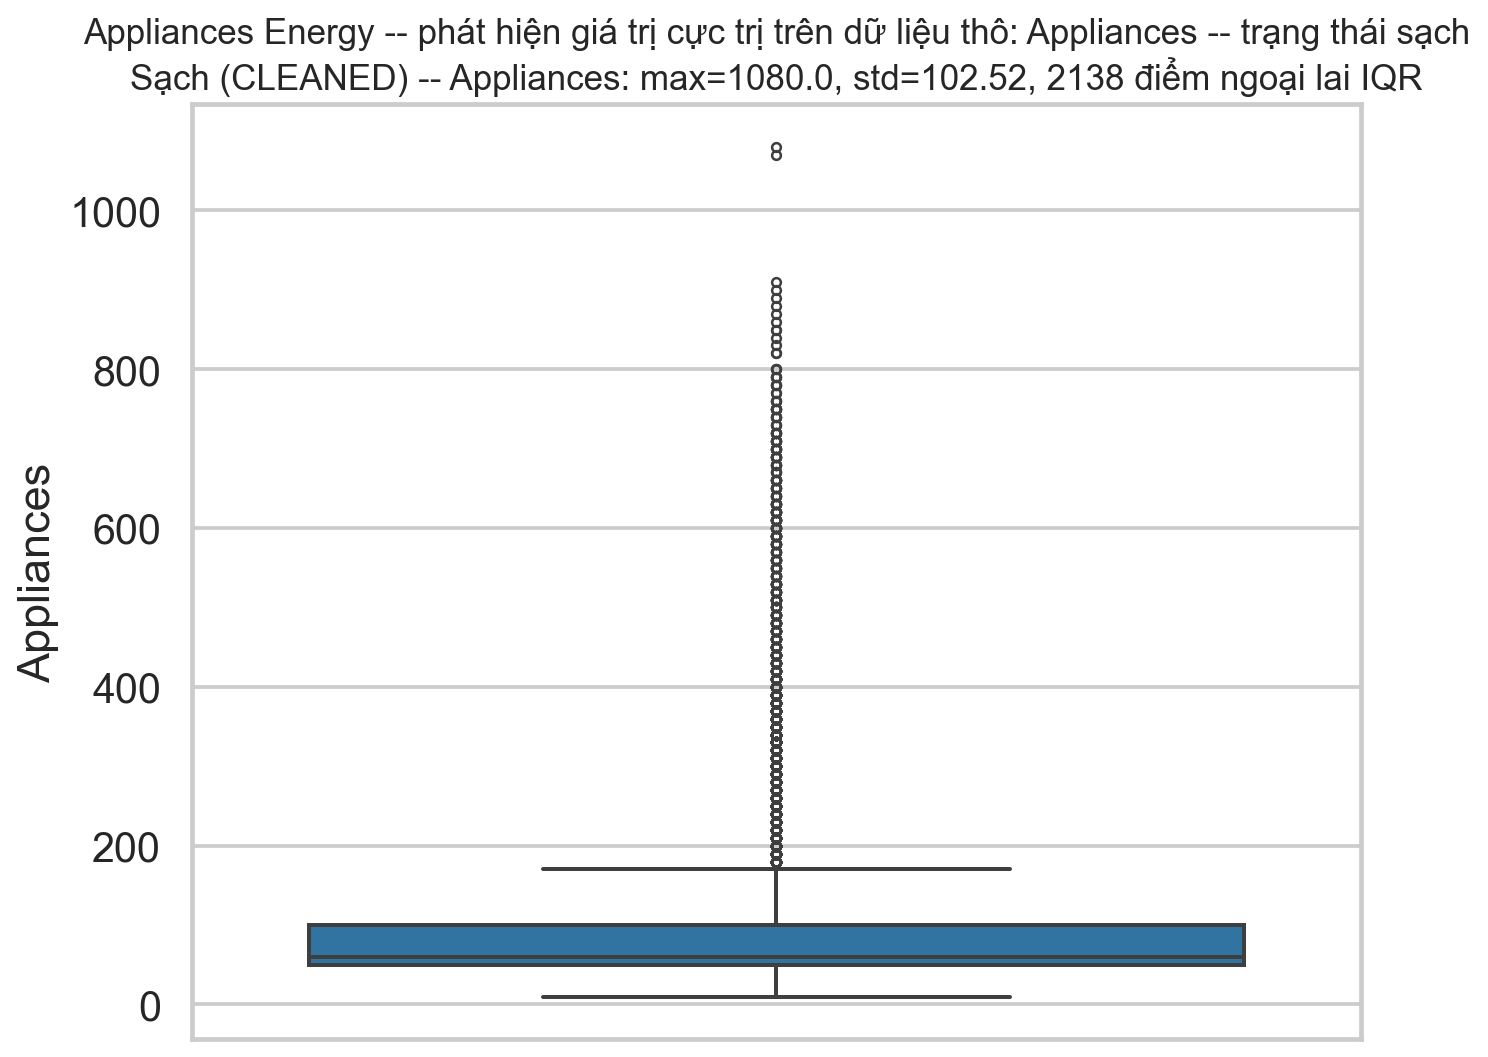
\includegraphics[width=0.72\textwidth]{images/ch3/appliances_energy_Appliances_boxplot_cleaned.png}
\captionsetup{justification=raggedright,singlelinecheck=false}
\caption[Boxplot \texttt{Appliances} sạch]{Boxplot \texttt{Appliances} ở \textbf{trạng thái sạch}: vì đây là target dự báo nên gần như giữ nguyên so với trạng thái thô (các đỉnh 1080 Wh được bảo toàn); chỉ các biến đầu vào \texttt{T\_out}, \texttt{RH\_1} mới bị clipping IQR.\\
\footnotesize Python source: \texttt{scripts/generate\_raw\_vs\_cleaned\_boxplots.py}.}
\label{fig:ch4_appliances_cleaned_boxplot}
\end{figure}

\textbf{Bước 1--2. Phân loại biến và thống kê mô tả.} Mọi biến đầu vào là Quantitative Continuous dạng chuỗi thời gian/cảm biến; \texttt{Appliances} là biến mục tiêu Continuous (regression).

\begin{table}[H]
\centering
\caption[Thống kê mô tả Appliances Energy]{Thống kê mô tả các chuỗi tiêu biểu Appliances Energy. Source: \texttt{outputs/tables/appliances\_energy\_summary.csv}.}
\label{tab:ch4_appliances_stats}
\small
\begin{tabular}{lrrrrr}
\toprule
Biến & Mean & Median & Std & Min & Max \\
\midrule
\texttt{Appliances} & 97.69 & 60.00 & 102.52 & 10.00 & 1080.00 \\
\texttt{lights} & 3.80 & 0.00 & 7.94 & 0.00 & 70.00 \\
\texttt{T1} & 21.69 & 21.60 & 1.61 & 16.79 & 26.26 \\
\texttt{RH\_1} & 40.26 & 39.66 & 3.98 & 27.02 & 63.36 \\
\texttt{T\_out} & 7.41 & 6.92 & 5.32 & -5.00 & 26.10 \\
\bottomrule
\end{tabular}
\end{table}

\begin{table}[H]
\centering
\caption[Thống kê thô/sạch Appliances Energy]{So sánh thống kê mô tả Appliances Energy ở hai trạng thái: \textbf{thô} và \textbf{sạch}. Lưu ý \texttt{Appliances} (target) \emph{không đổi} vì không clipping; các biến đầu vào thay đổi nhẹ do clipping IQR. Source: \texttt{outputs/tables/appliances\_energy\_summary.csv}.}
\label{tab:ch4_appliances_stats_raw_clean}
\footnotesize
\setlength{\tabcolsep}{4pt}
\begin{tabular}{lcrrrrr}
\toprule
Biến & Trạng thái & Mean & Median & Std & Min & \textbf{Max} \\
\midrule
\texttt{Appliances} & thô & 97.69 & 60.00 & 102.52 & 10.00 & 1080.00 \\
 (target, không clip) & sạch & 97.69 & 60.00 & 102.52 & 10.00 & 1080.00 \\
\midrule
\texttt{T1} & thô & 21.69 & 21.60 & 1.61 & 16.79 & \textbf{26.26} \\
 & sạch & 21.69 & 21.60 & 1.58 & 18.00 & \textbf{25.36} \\
\midrule
\texttt{RH\_1} & thô & 40.26 & 39.66 & 3.98 & 27.02 & \textbf{63.36} \\
 & sạch & 40.25 & 39.66 & 3.94 & 28.73 & \textbf{51.67} \\
\midrule
\texttt{T\_out} & thô & 7.41 & 6.92 & 5.32 & -5.00 & \textbf{26.10} \\
 & sạch & 7.37 & 6.92 & 5.20 & -5.00 & \textbf{20.50} \\
\bottomrule
\end{tabular}
\end{table}

\textit{Nhận xét thô/sạch.} Khác với Nhóm A, sự thay đổi ở Appliances Energy rất nhỏ vì các biến đầu vào (nhiệt độ, độ ẩm) ít có ngoại lai; clipping chỉ nén một vài giá trị cực trị ở biên (ví dụ \texttt{RH\_1} max 63.36$\to$51.67, \texttt{T\_out} max 26.10$\to$20.50). Quan trọng nhất, biến mục tiêu \texttt{Appliances} \emph{giữ nguyên hoàn toàn} ở cả hai trạng thái -- đây là quy tắc cốt lõi trong dự báo chuỗi thời gian: không clipping target để mô hình học đúng giá trị thực, kể cả các đỉnh tiêu thụ 1080 Wh.

\begin{table}[H]
\centering
\caption[Thông tin thời gian Appliances Energy]{Thông tin thời gian của chuỗi Appliances Energy. Source: \texttt{outputs/tables/appliances\_energy\_time\_info.csv}.}
\label{tab:ch4_appliances_time_info}
\small
\begin{tabular}{lr}
\toprule
Chỉ tiêu & Giá trị \\
\midrule
Bắt đầu & 2016-01-11 17:00:00 \\
Kết thúc & 2016-05-27 18:00:00 \\
Số quan sát & 19\,735 \\
Tần suất mode & 10 phút \\
\bottomrule
\end{tabular}
\end{table}

\textbf{Bước 3. Trực quan hóa (line chart, rolling, điền khuyết, raw vs log, differencing, ridgeline).}

\begin{figure}[H]\centering
\begin{subfigure}{0.90\textwidth}\centering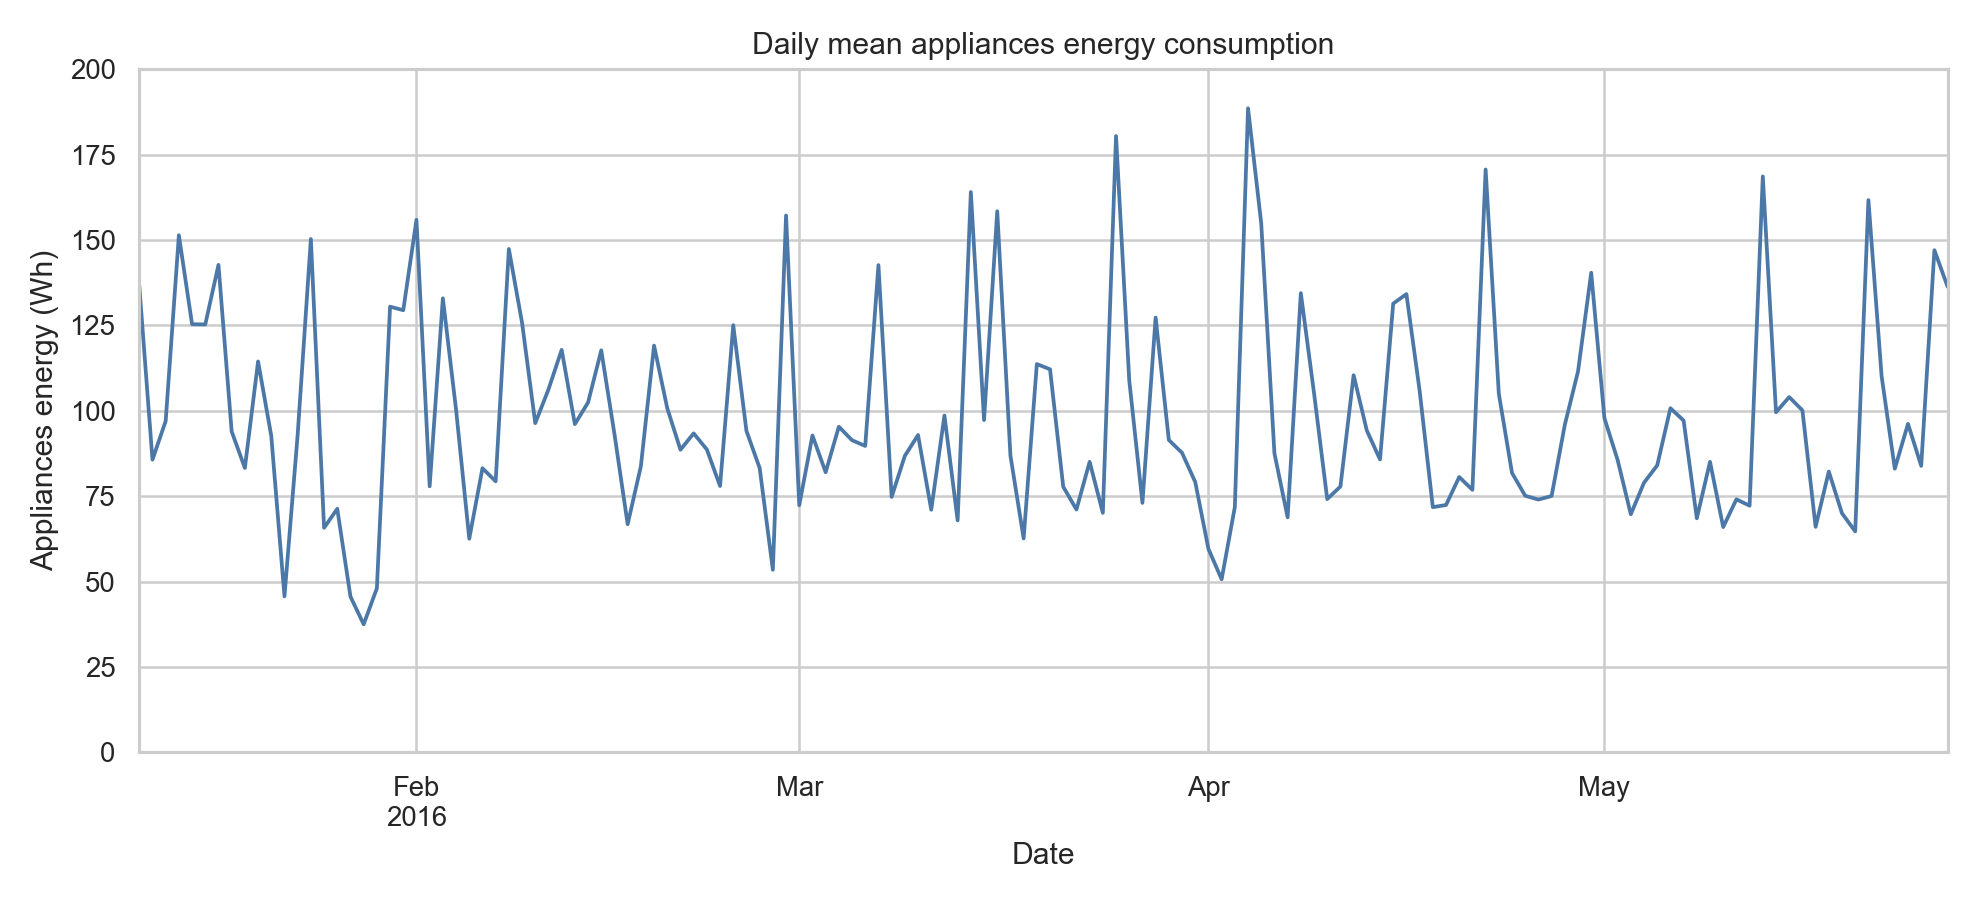
\includegraphics[width=\textwidth]{images/ch3/appliances_energy_daily_line.png}\caption{Python -- Daily line chart}\end{subfigure}
\par\medskip
\begin{subfigure}{0.90\textwidth}\centering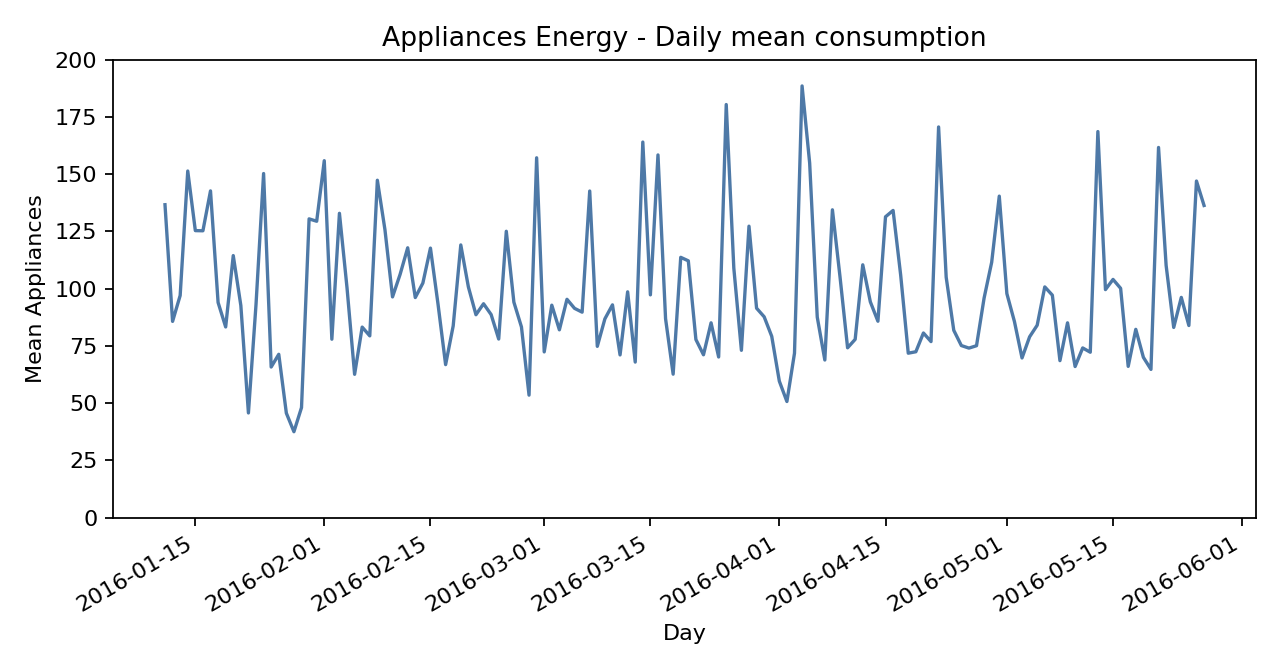
\includegraphics[width=\textwidth]{images/ch3/excel_appliances_daily_line_preview.png}\caption{Excel -- Daily line chart}\end{subfigure}
\caption[Line chart Appliances Energy: Python và Excel]{Xu hướng tiêu thụ điện trung bình theo ngày.\\
\footnotesize Python source: \texttt{src/analyze\_appliances\_energy.py}. Excel source/workbook: \texttt{src/create\_excel\_visualizations.py}, \texttt{excel/excel\_visualization\_comparison\_native.xlsx}, sheet \texttt{Appliances Daily}.}
\label{fig:ch4_appliances_daily_line}
\end{figure}
\textbf{Nhận xét Hình \ref{fig:ch4_appliances_daily_line}.} Line chart cho thấy mức tiêu thụ dao động mạnh theo ngày, không phù hợp chia train/test ngẫu nhiên. Cần giữ thứ tự thời gian để tránh rò rỉ thông tin tương lai.

\begin{figure}[H]\centering
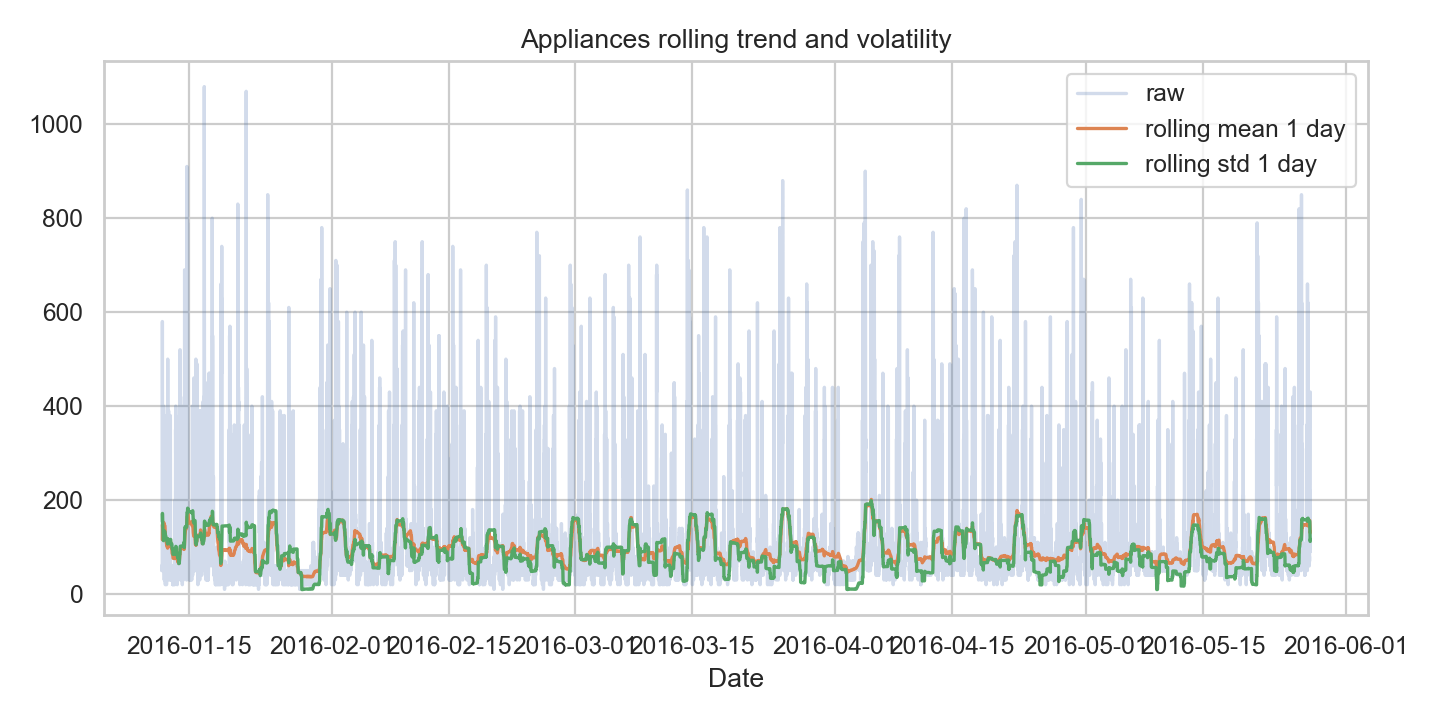
\includegraphics[width=0.90\textwidth]{images/ch3/appliances_energy_rolling_trend.png}
\caption[Rolling statistics Appliances Energy]{Rolling mean và rolling standard deviation 1 ngày của \texttt{Appliances}.\\
\footnotesize Python source: \texttt{scripts/generate\_group\_b\_figures.py}.}
\label{fig:ch4_appliances_rolling}
\end{figure}
\textbf{Nhận xét Hình \ref{fig:ch4_appliances_rolling}.} Rolling mean làm rõ xu hướng nền, còn rolling std cho thấy phương sai thay đổi theo thời gian. Đây là dấu hiệu chuỗi không hoàn toàn dừng.

\begin{figure}[H]\centering
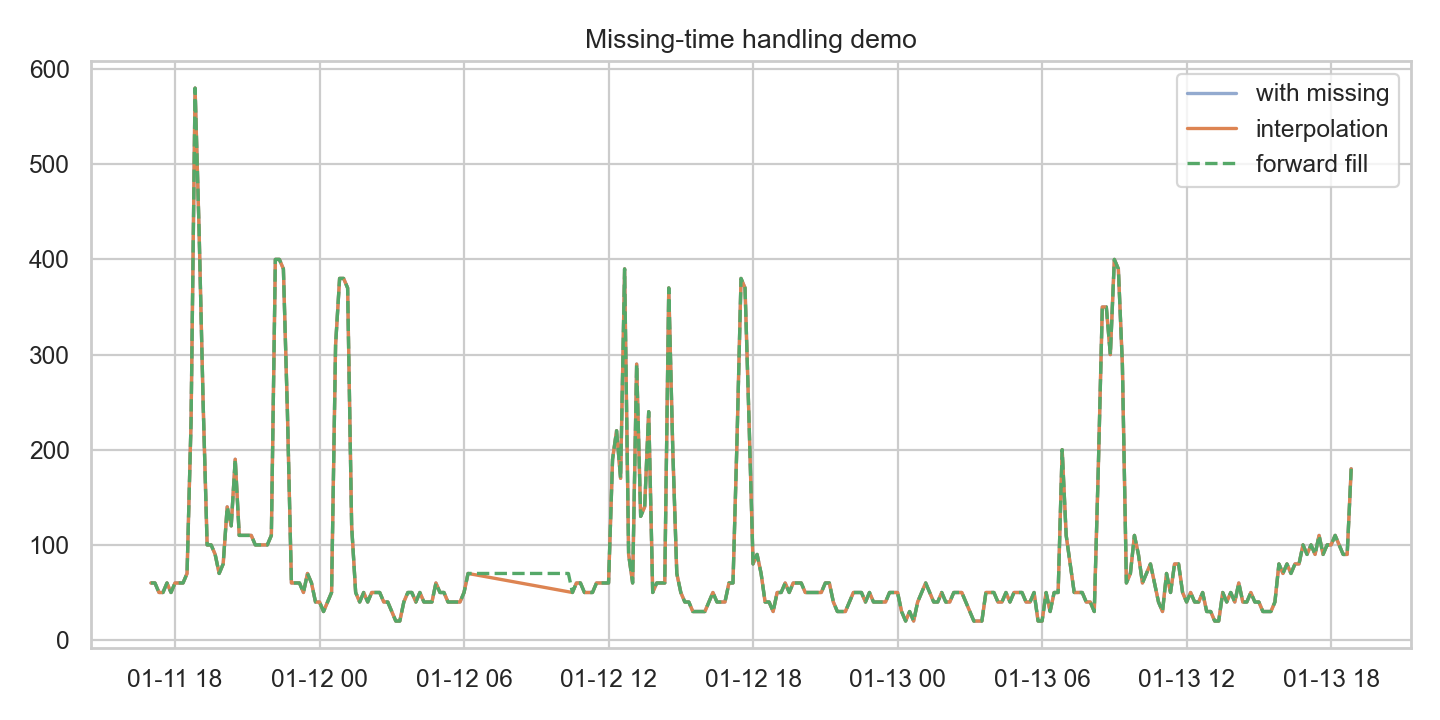
\includegraphics[width=0.90\textwidth]{images/ch3/appliances_energy_missing_interpolation_ffill.png}
\caption[Điền khuyết thời gian Appliances Energy]{Minh họa xử lý missing theo thời gian bằng interpolation và forward fill.\\
\footnotesize Python source: \texttt{scripts/generate\_group\_b\_figures.py}.}
\label{fig:ch4_appliances_missing_fill}
\end{figure}
\textbf{Nhận xét Hình \ref{fig:ch4_appliances_missing_fill}.} Interpolation tạo đường chuyển tiếp mượt giữa hai điểm quan sát, còn forward fill giữ giá trị gần nhất. Ở trạng thái thô, các khoảng Null/NaN tạo đoạn rỗng hoặc đứt gãy trên line chart; sau xử lý, chuỗi liền mạch hơn nên rolling mean, rolling std và mô hình dự báo không bị ngắt do thiếu điểm. Với chuỗi cảm biến 10 phút, interpolation phù hợp khi missing ngắn; forward fill phù hợp khi trạng thái vật lý ít thay đổi.

\begin{figure}[H]\centering
\begin{subfigure}{0.90\textwidth}\centering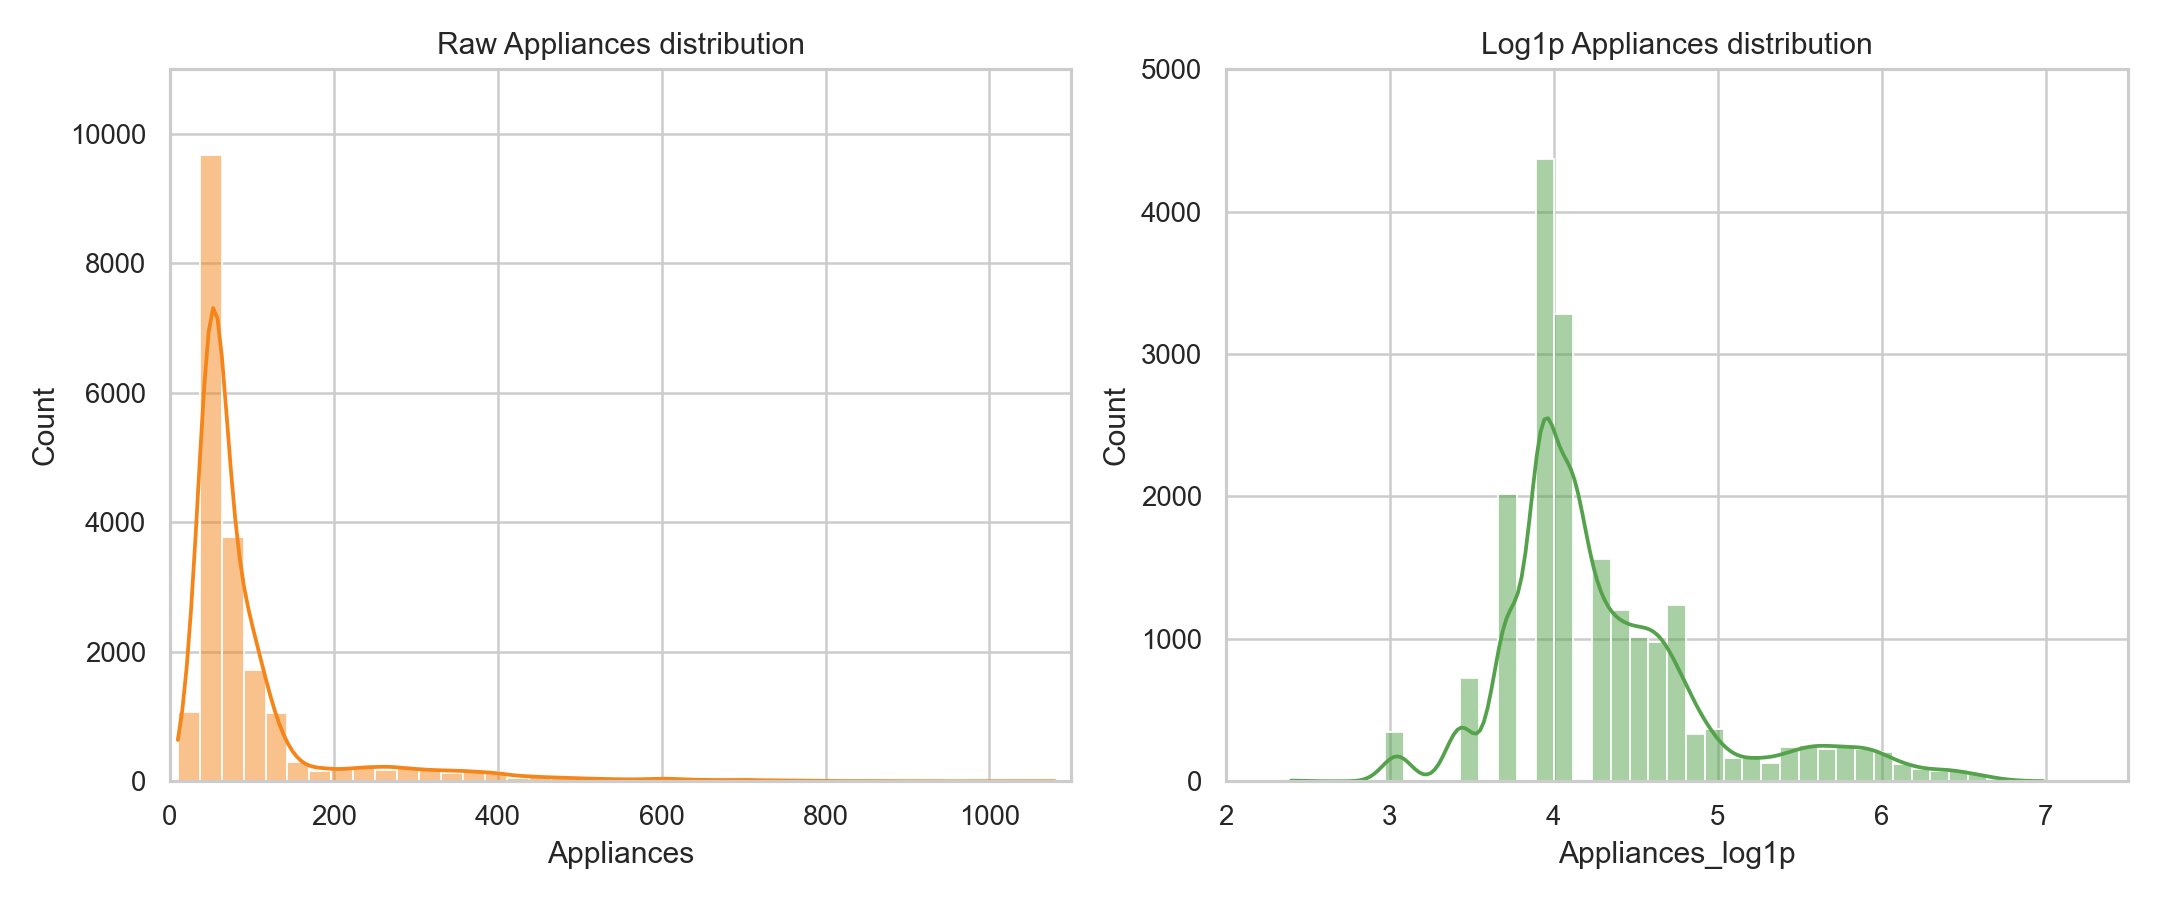
\includegraphics[width=\textwidth]{images/ch3/appliances_energy_distribution_raw_vs_log.png}\caption{Python -- Raw vs log1p}\end{subfigure}
\par\medskip
\begin{subfigure}{0.90\textwidth}\centering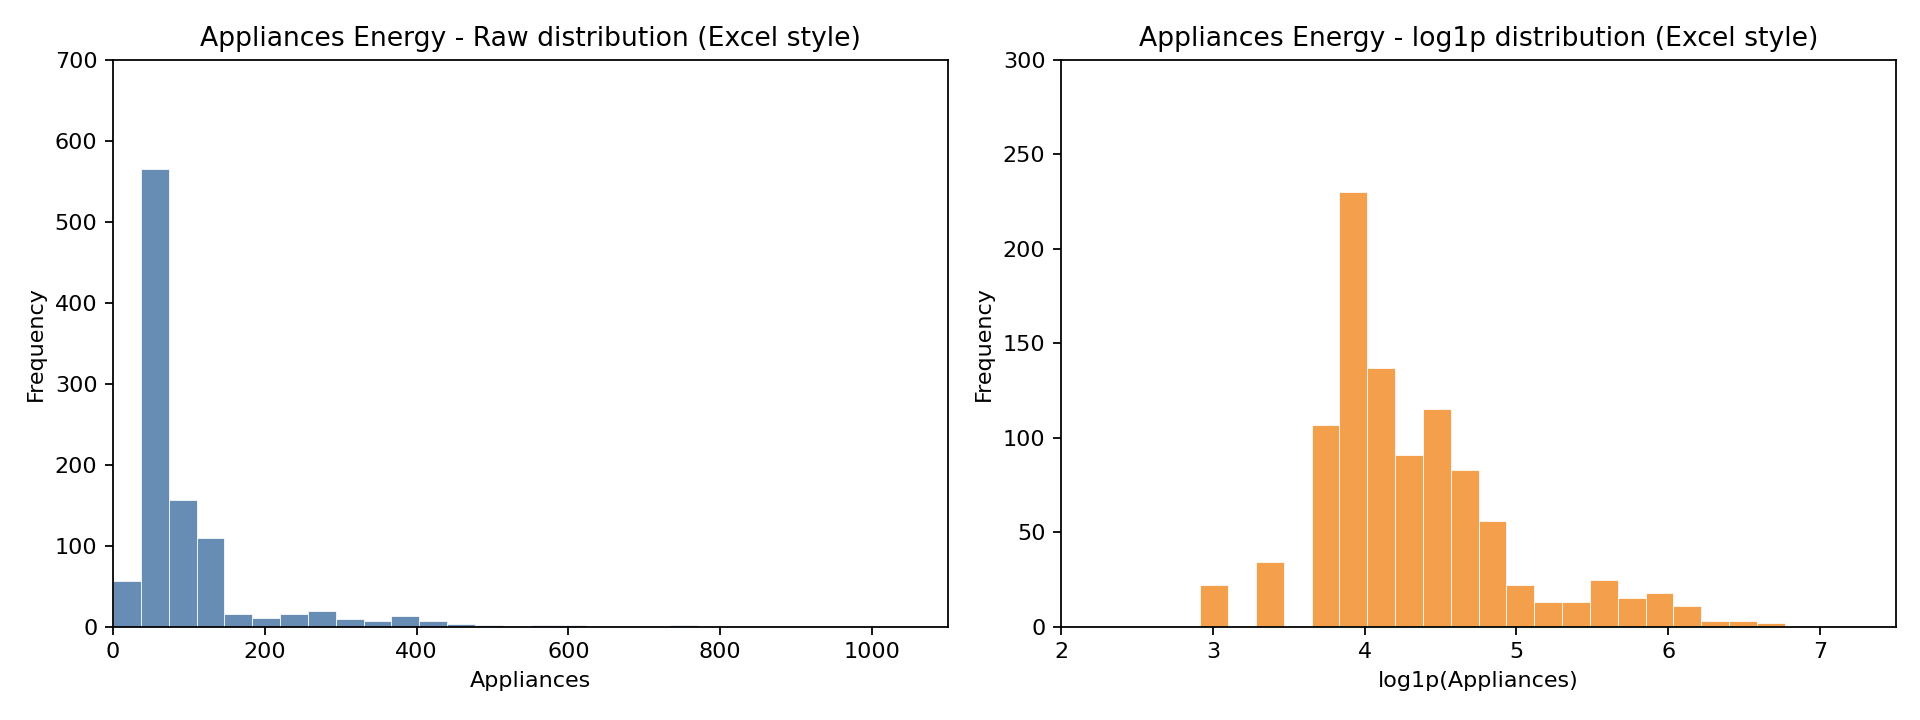
\includegraphics[width=\textwidth]{images/ch3/excel_appliances_raw_vs_log_hist_preview.png}\caption{Excel -- Raw vs log1p}\end{subfigure}
\caption[Log-transform Appliances Energy: Python và Excel]{Biến đổi \texttt{log1p} để giảm lệch phải của \texttt{Appliances}.\\
\footnotesize Python source: \texttt{src/analyze\_appliances\_energy.py}. Excel source/workbook: \texttt{src/create\_excel\_visualizations.py}, \texttt{excel/excel\_visualization\_comparison\_native.xlsx}, sheet \texttt{Appliances Histogram}.}
\label{fig:ch4_appliances_log}
\end{figure}
\textbf{Nhận xét Hình \ref{fig:ch4_appliances_log}.} Phân phối gốc lệch phải mạnh do các đỉnh tiêu thụ cao. \texttt{log1p} nén đuôi phải, giúp phương sai ổn định hơn.

\begin{figure}[H]\centering
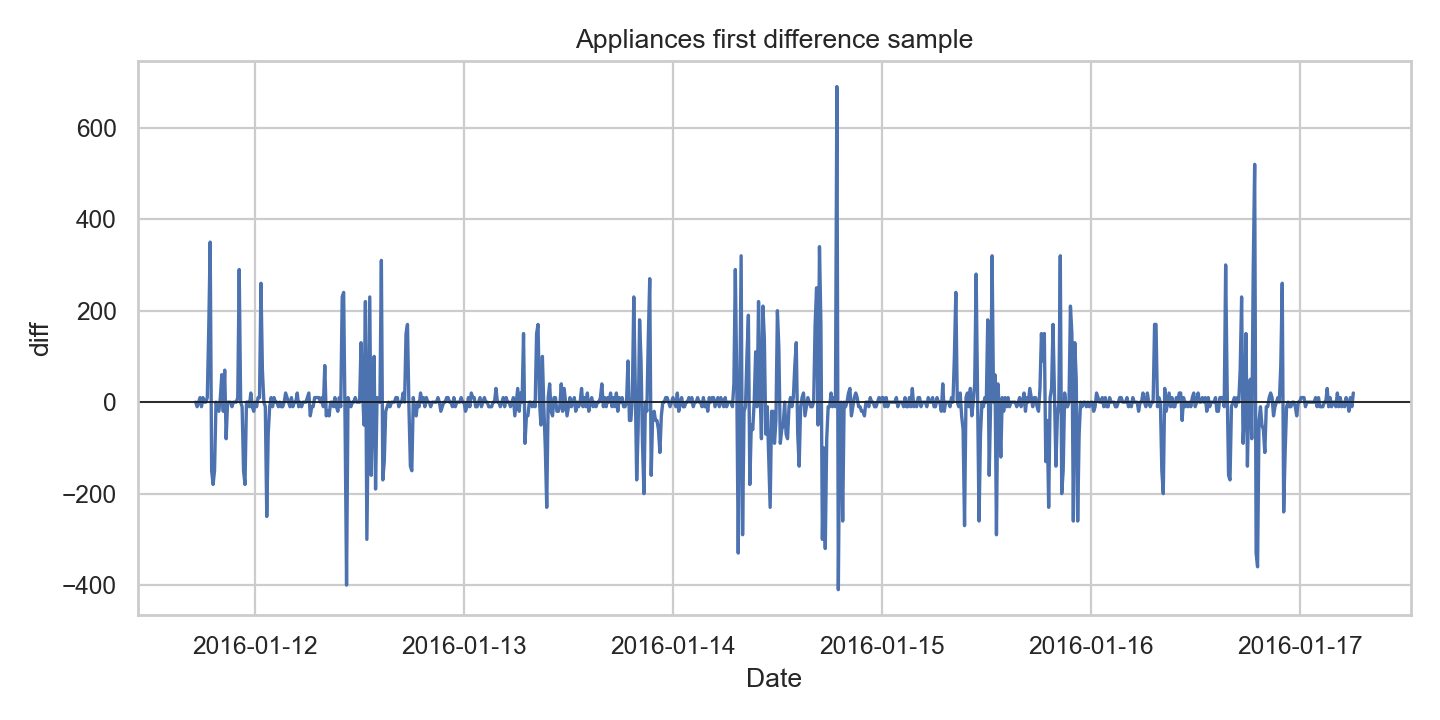
\includegraphics[width=0.90\textwidth]{images/ch3/appliances_energy_differencing_line.png}
\caption[Differencing Appliances Energy]{Sai phân bậc một của \texttt{Appliances}.\\
\footnotesize Python source: \texttt{scripts/generate\_group\_b\_figures.py}.}
\label{fig:ch4_appliances_diff}
\end{figure}
\textbf{Nhận xét Hình \ref{fig:ch4_appliances_diff}.} Differencing đưa chuỗi về dao động quanh 0, giúp nhấn mạnh thay đổi ngắn hạn thay vì mức tuyệt đối.

\begin{figure}[H]\centering
\begin{subfigure}{0.90\textwidth}\centering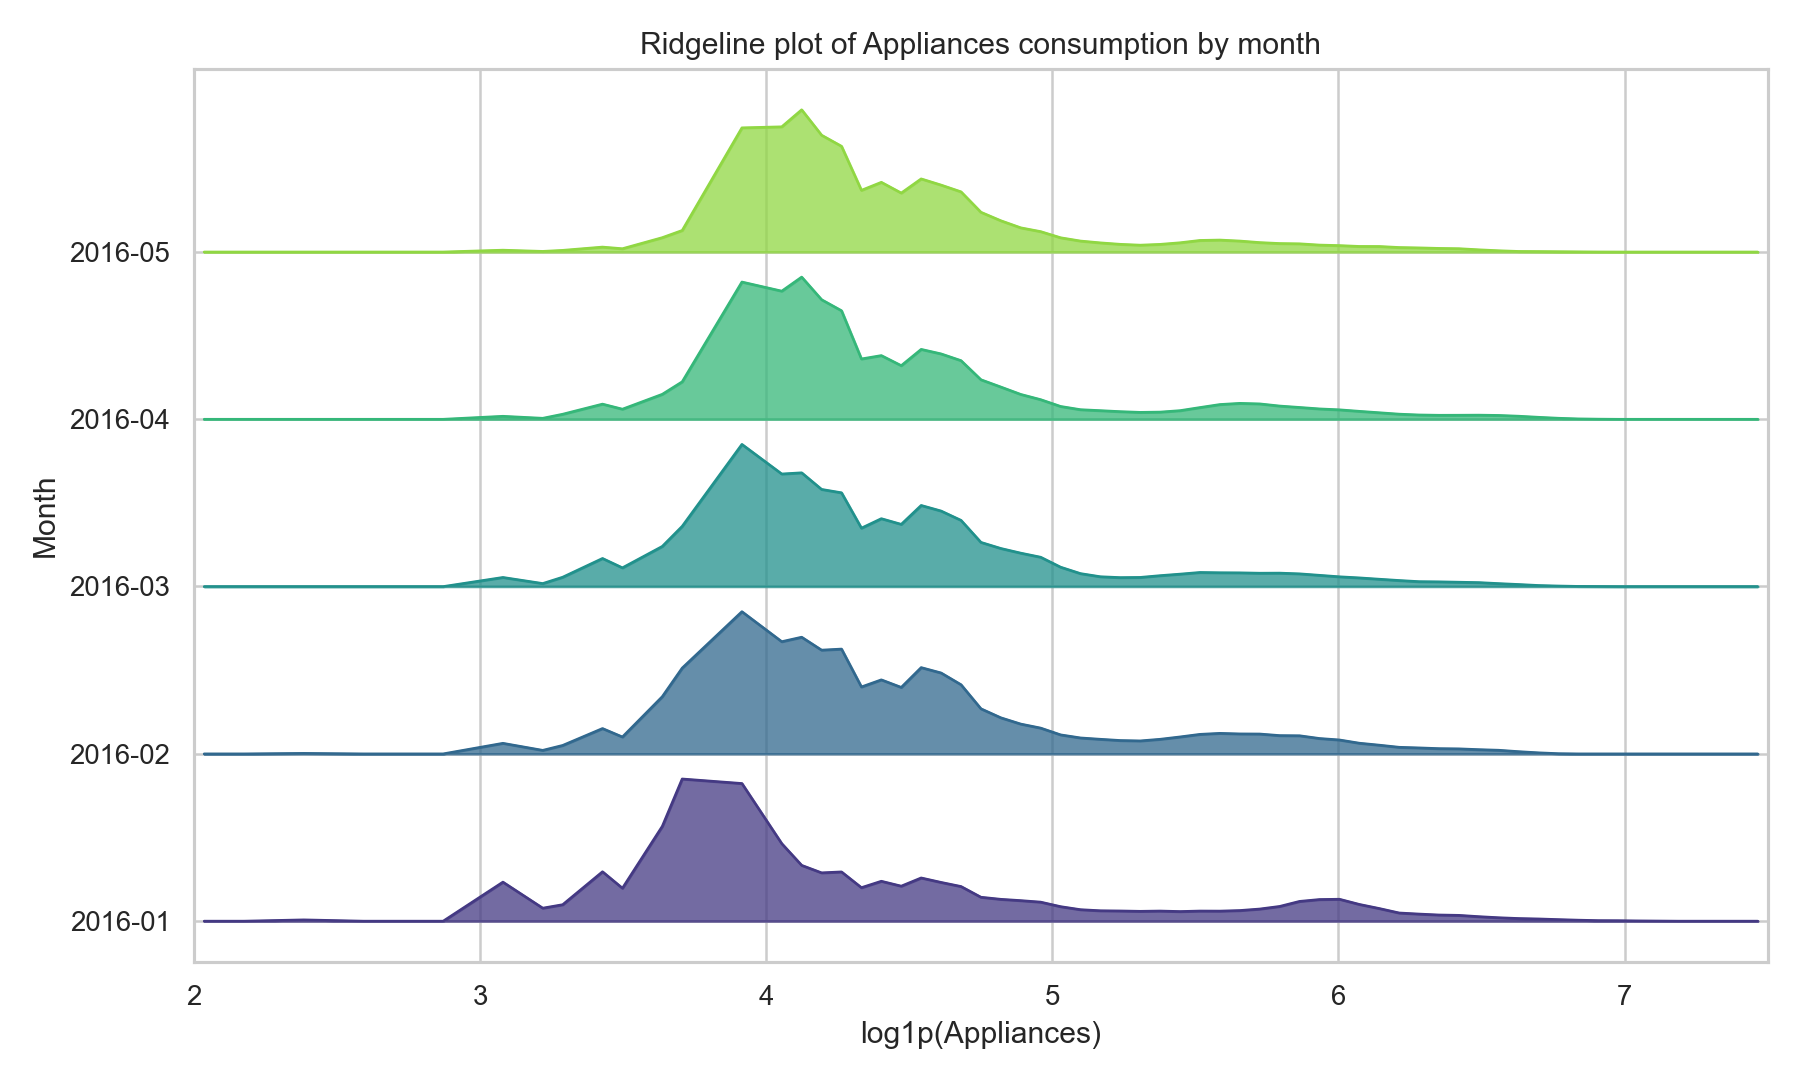
\includegraphics[width=\textwidth]{images/ch3/appliances_energy_monthly_ridgeline.png}\caption{Python -- Monthly ridgeline}\end{subfigure}
\caption[Mùa vụ Appliances Energy]{Phân phối \texttt{log1p(Appliances)} theo tháng.\
\footnotesize Python source: \texttt{src/analyze\_appliances\_energy.py}.\
}\label{fig:ch4_appliances_seasonality}
\end{figure}
\textbf{Nhận xét Hình \ref{fig:ch4_appliances_seasonality}.} Ridgeline cho thấy hình dạng phân phối thay đổi theo tháng, gợi ý ảnh hưởng mùa vụ và điều kiện thời tiết ngoài trời.

\textbf{Bước 4. So sánh trước--sau biến đổi chuỗi.} Trạng thái thô và trạng thái sạch của Appliances Energy khác ở ba phép biến đổi chính, mỗi phép được minh chứng bằng một biểu đồ: (1) \emph{điền khuyết} -- Hình~\ref{fig:ch4_appliances_missing_fill} cho thấy line chart của chuỗi thô có thể đứt gãy tại các NaN, còn sau interpolation/forward fill thì liền mạch; (2) \emph{log-transform} -- Hình~\ref{fig:ch4_appliances_log} đặt histogram \texttt{Appliances} thô (lệch phải mạnh, đuôi tới 1080) cạnh histogram \texttt{log1p(Appliances)} (gần đối xứng hơn); (3) \emph{differencing} -- Hình~\ref{fig:ch4_appliances_diff} cho thấy chuỗi sai phân dao động quanh 0. \textbf{Nhận xét so sánh:} chuỗi thô có std rất lớn (102.52) và phân phối đỉnh lệch, chuỗi sau log-transform có std nhỏ hơn rõ và gần chuẩn hơn -- đây là điều kiện quan trọng cho các mô hình tuyến tính và ARIMA. Differencing làm mất một bậc tự do nhưng loại bỏ trend, giúp chuỗi dừng hơn. Vì dữ liệu gốc không có missing thực, ``trạng thái sạch'' ở đây chủ yếu là \emph{biến đổi chuỗi} chứ không phải điền khuyết; báo cáo trình bày trung thực điều này.

\subsubsection{Human Activity Recognition Using Smartphones}

HAR có 10\,299 quan sát và 561 đặc trưng cảm biến đã trích xuất. Năm chuỗi/feature chọn để phân tích gồm \texttt{f001\_tBodyAcc-mean()-X}, \texttt{f002\_tBodyAcc-mean()-Y}, \texttt{f003\_tBodyAcc-mean()-Z}, \texttt{f004\_tBodyAcc-std()-X}, \texttt{f005\_tBodyAcc-std()-Y}.

\textbf{Trạng thái dữ liệu thô (chưa làm sạch).} HAR của UCI đã được \emph{tiền xử lý sẵn} ở nguồn: tín hiệu gia tốc/gyro được lọc nhiễu, chia cửa sổ trượt 2.56~s, trích xuất 561 đặc trưng và chuẩn hóa trong khoảng $[-1,1]$. Do đó bộ dữ liệu \emph{không có ô khuyết thiếu} và không yêu cầu điền khuyết/clipping ở giai đoạn này; ``trạng thái thô'' và ``trạng thái sạch'' gần như trùng nhau. Dù vậy, vì đây là dữ liệu chuỗi cảm biến, quy trình Nhóm B vẫn kiểm tra hai điều kiện thời gian: (1) \emph{đứt gãy trên line chart} -- Hình~\ref{fig:ch4_har_line} cho thấy chuỗi liền mạch, không có khoảng NaN cần điền bằng forward/backward fill hay linear interpolation; (2) \emph{biến đổi chuỗi} -- vì các feature đã được chuẩn hóa $[-1,1]$ và trích xuất theo cửa sổ, log-transform và differencing không mang thêm giá trị ở cấp độ feature; thay vào đó, rolling statistics có thể dùng để quan sát xu hướng theo đoạn hoạt động.

\textit{Phát hiện trên dữ liệu thô (boxplot).} Trên boxplot 5 feature theo hoạt động (Hình~\ref{fig:ch4_har_box}), vẫn xuất hiện các điểm rời rạc ngoài râu IQR ở các feature gia tốc. Tuy nhiên, các điểm này thường là \emph{chuyển động thực sự mãnh liệt} (ví dụ chạy WALKING, nhảy) chứ không phải lỗi đo, đặc biệt feature \texttt{f001...X} ở nhóm hoạt động động có phân bố rộng và nhiều ngoại biên hơn nhóm tĩnh (SITTING/STANDING/LAYING). Vì vậy chúng \emph{không nên loại bỏ cơ học}; clipping sẽ làm mất chính tín hiệu cần phân loại.

\textit{Đứt gãy trên line chart.} Hình~\ref{fig:ch4_har_line} cho thấy line chart của 5 feature liền mạch (không có đoạn đứt), xác nhận dữ liệu đã hoàn chỉnh.

\textbf{Bước 1--2. Phân loại biến và thống kê.} Các feature là Quantitative Continuous đã chuẩn hóa $[-1,1]$; biến mục tiêu \texttt{Activity} là Qualitative nominal (6 lớp: WALKING, WALKING\_UPSTAIRS, WALKING\_DOWNSTAIRS, SITTING, STANDING, LAYING).

\textbf{Bước 3. Trực quan hóa (phân bố hoạt động, line chart, boxplot theo hoạt động, heatmap tương quan).}

\begin{figure}[H]\centering
\begin{subfigure}{0.90\textwidth}\centering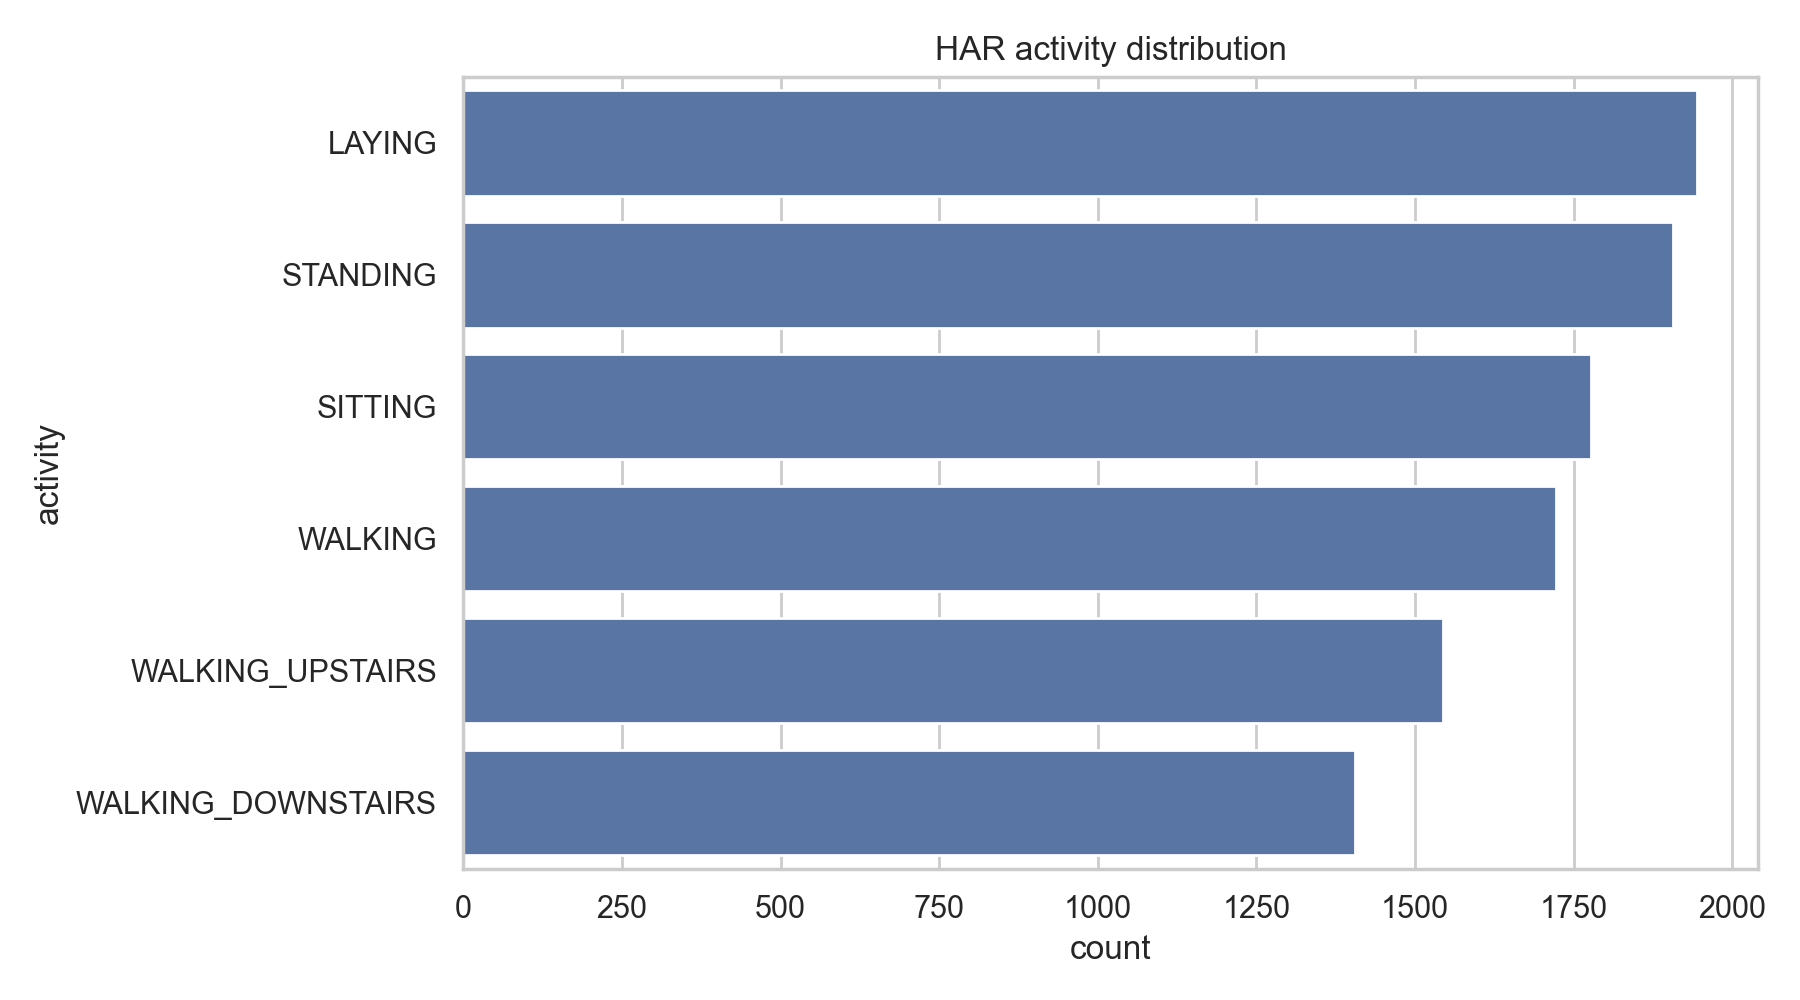
\includegraphics[width=\textwidth]{images/ch3/har_activity_distribution.png}\caption{Python -- Activity distribution}\end{subfigure}
\caption[Phân bố hoạt động HAR]{Tần suất các hoạt động trong HAR.\
\footnotesize Python source: \texttt{src/analyze\_har.py}.\
}\label{fig:ch4_har_activity}
\end{figure}
\textbf{Nhận xét Hình \ref{fig:ch4_har_activity}.} Các lớp hoạt động tương đối cân bằng, thuận lợi cho phân loại nhiều lớp; vẫn cần kiểm tra từng lớp động/tĩnh vì tín hiệu cảm biến có độ biến thiên khác nhau.

\begin{figure}[H]\centering
\begin{subfigure}{0.90\textwidth}\centering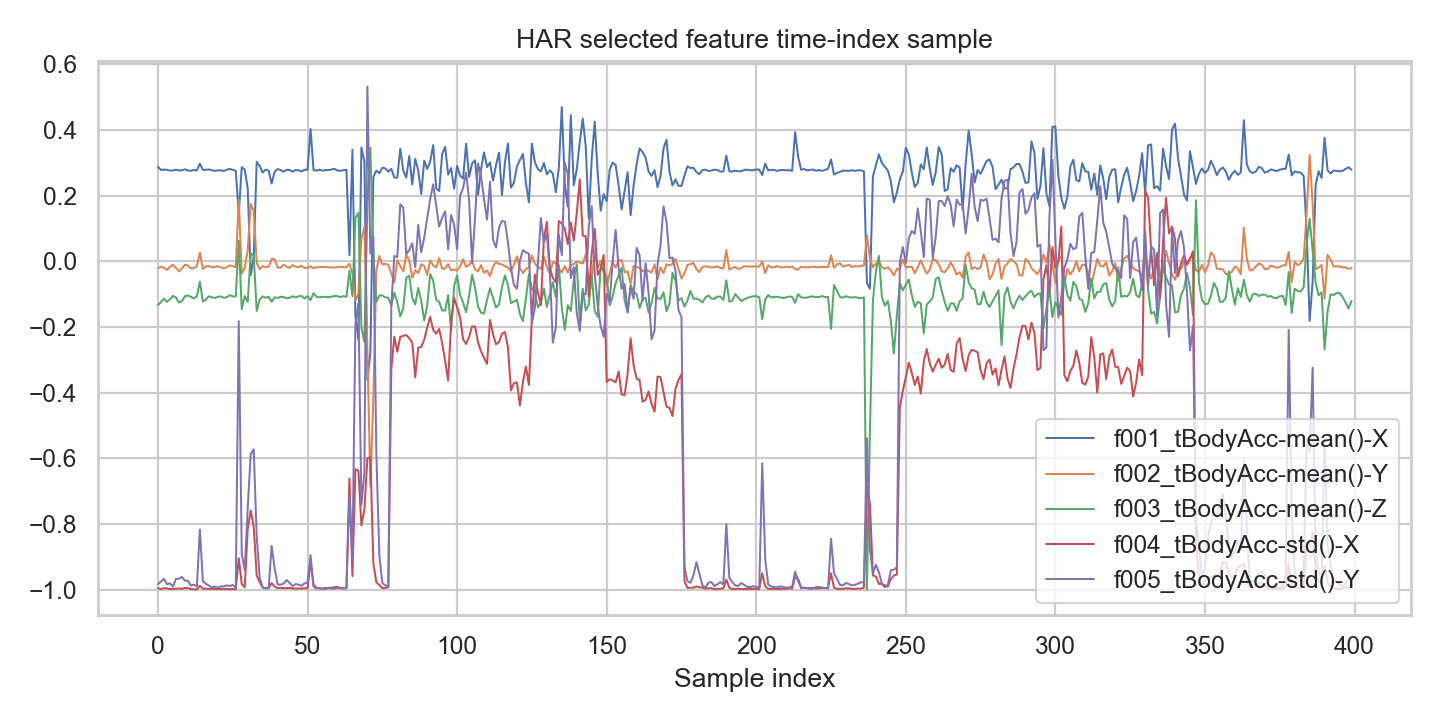
\includegraphics[width=\textwidth]{images/ch3/har_selected_feature_line.png}\caption{Python -- Feature line sample}\end{subfigure}
\caption[Line chart HAR]{Line chart theo index mẫu của 5 feature HAR đã chọn.\
\footnotesize Python source: \texttt{scripts/generate\_group\_b\_figures.py}.\
}\label{fig:ch4_har_line}
\end{figure}
\textbf{Nhận xét Hình \ref{fig:ch4_har_line}.} Line chart cho thấy các feature tăng/giảm theo đoạn hoạt động; vì vậy khi chia dữ liệu cần chú ý subject và activity block, không chỉ coi mẫu là độc lập tuyệt đối.

\begin{figure}[H]\centering
\begin{subfigure}{0.90\textwidth}\centering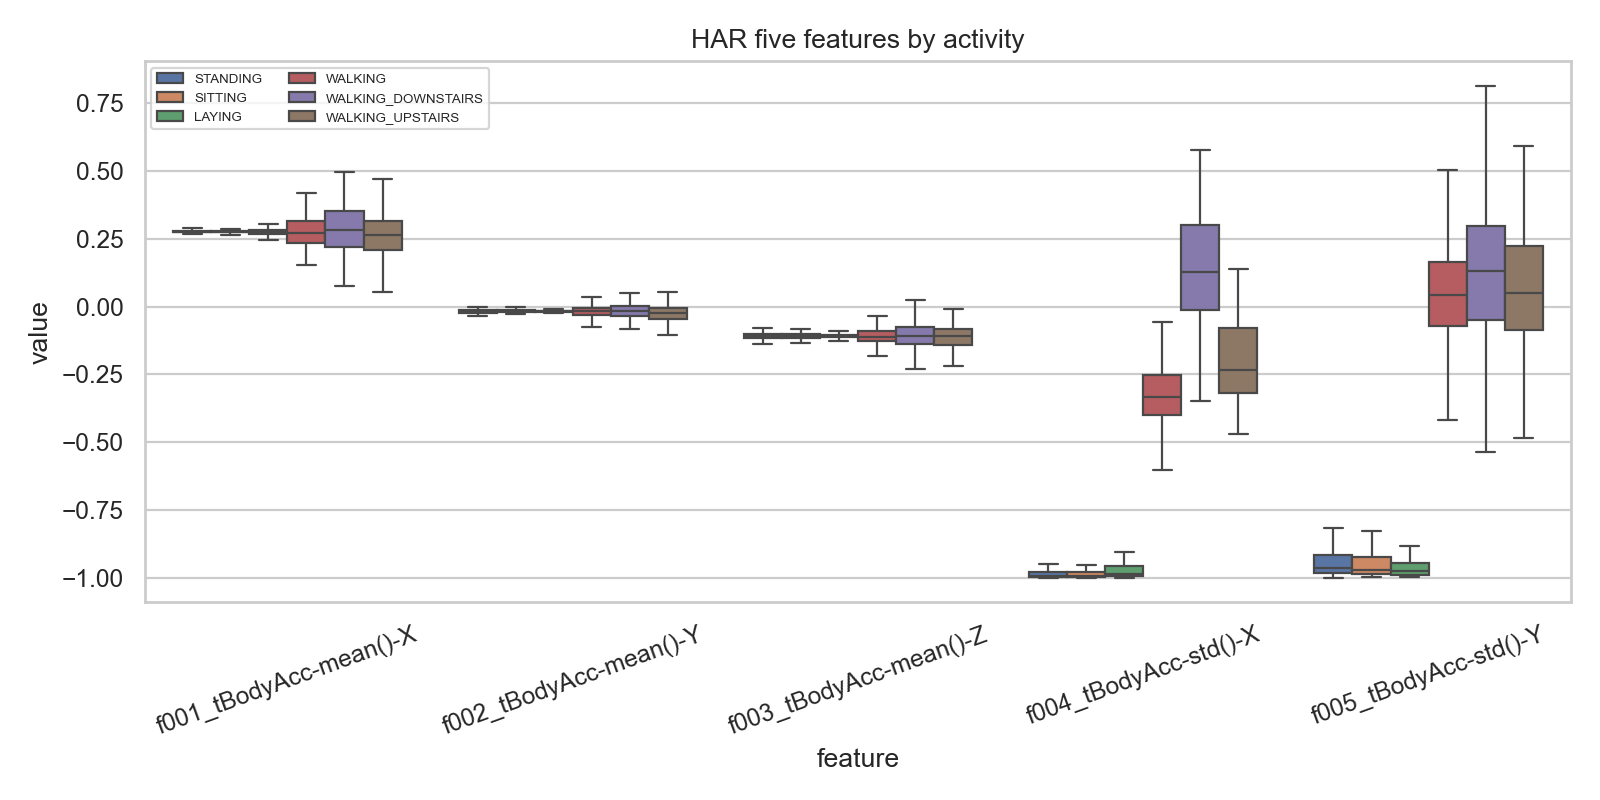
\includegraphics[width=\textwidth]{images/ch3/har_five_feature_boxplot.png}\caption{Python -- Boxplot 5 features}\end{subfigure}
\caption[Boxplot HAR]{Boxplot 5 feature HAR theo hoạt động.\
\footnotesize Python source: \texttt{scripts/generate\_group\_b\_figures.py}.\
}\label{fig:ch4_har_box}
\end{figure}
\textbf{Nhận xét Hình \ref{fig:ch4_har_box}.} Feature mean/std tách rõ giữa nhóm hoạt động tĩnh và động. Các giá trị ngoại biên có thể là chuyển động thực, không nên loại bỏ cơ học.

\begin{figure}[H]\centering
\begin{subfigure}{0.90\textwidth}\centering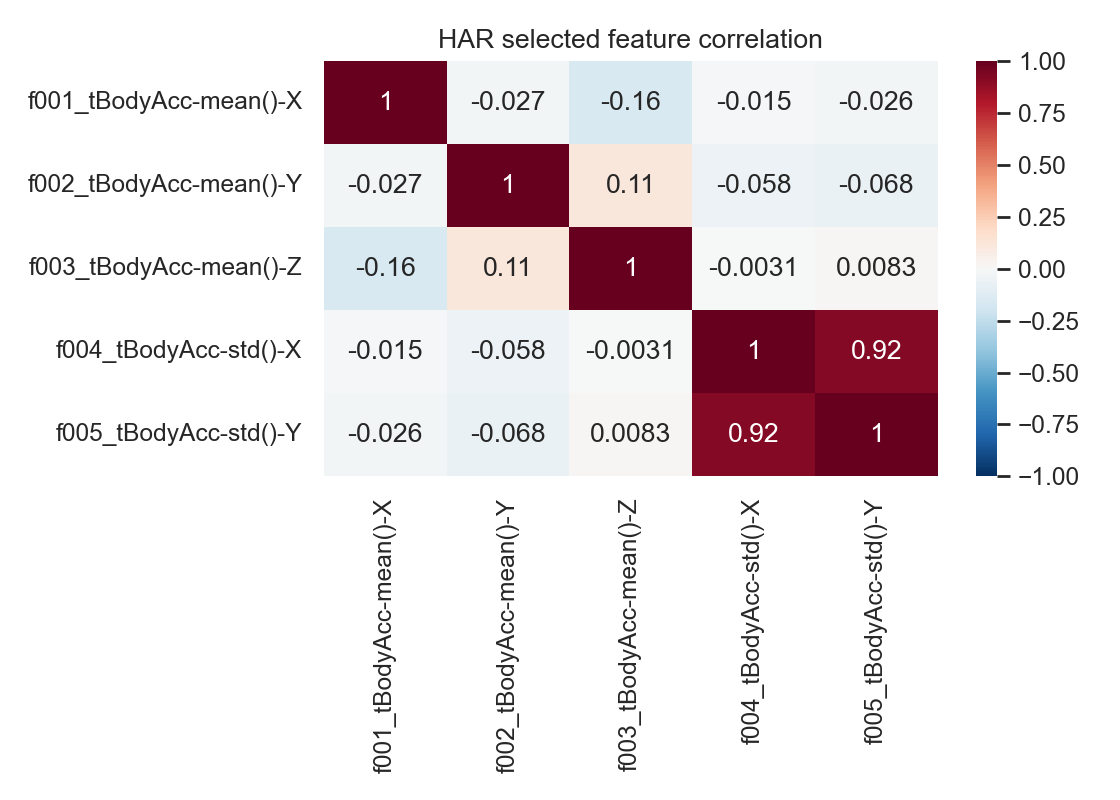
\includegraphics[width=\textwidth]{images/ch3/har_selected_feature_correlation_heatmap.png}\caption{Python -- Correlation heatmap}\end{subfigure}
\caption[Heatmap HAR]{Heatmap tương quan 5 feature HAR.\
\footnotesize Python source: \texttt{scripts/generate\_group\_b\_figures.py}.\
}\label{fig:ch4_har_corr}
\end{figure}
\textbf{Nhận xét Hình \ref{fig:ch4_har_corr}.} Các trục gia tốc có tương quan nhất định, nhưng không hoàn toàn trùng nhau; giữ nhiều trục giúp mô hình nhận diện hướng chuyển động.

\textbf{Bước 4. So sánh trước--sau.} Vì HAR đã chuẩn hóa sẵn và không có khuyết thiếu, ``trạng thái sạch'' không khác biệt đáng kể so với ``trạng thái thô'' -- điều này \emph{chính là một kết luận có giá trị}: dữ liệu cảm biến chất lượng cao, sẵn sàng cho mô hình mà không cần thêm làm sạch. Bài học rút ra cho mô hình là giữ lại các điểm ngoại biên mang ý nghĩa chuyển động, và chia train/test theo subject để tránh rò rỉ thông tin.

\subsubsection{MHEALTH}

MHEALTH là dữ liệu cảm biến đeo trên cơ thể. Sáu chuỗi chọn phân tích gồm \texttt{sensor\_01}, \texttt{sensor\_02}, \texttt{sensor\_03}, \texttt{sensor\_10}, \texttt{sensor\_11}, \texttt{sensor\_12}; các chuỗi này đại diện cho nhiều kênh cảm biến và hoạt động.

\textbf{Trạng thái dữ liệu thô (chưa làm sạch).} MHEALTH là tín hiệu cảm biến thô đã ghi liên tục ở 50~Hz; bộ dữ liệu \emph{không có ô khuyết thiếu} đáng kể. Trên line chart 6 sensor (Hình~\ref{fig:ch4_mhealth_line}), chuỗi \emph{liền mạch, không có đoạn đứt gãy}, xác nhận dữ liệu thu thập hoàn chỉnh -- do đó không cần áp dụng forward/backward fill hay linear interpolation.

\textit{Phát hiện trên dữ liệu thô (boxplot / line chart).} Trên boxplot sensor theo hoạt động (Hình~\ref{fig:ch4_mhealth_box}), xuất hiện nhiều điểm rời rạc ngoài râu IQR, đặc biệt ở các sensor gia tốc (\texttt{sensor\_01..03}). Các đỉnh đột biến này thường là \emph{chuyển động đột ngột hợp lệ} (ví dụ đá chân, gập người, nhảy), nên không nên clipping cơ học -- làm vậy sẽ mất chính các sự kiện hoạt động cần nhận dạng; dao động ngắn hạn mạnh trên line chart phản ánh chuyển động cơ thể thực.

\textbf{Làm sạch dữ liệu.} Vì dữ liệu cảm biến không có khuyết thiếu và các ngoại lai mang ý nghĩa chuyển động, các bước ``làm sạch'' tập trung vào \emph{biến đổi chuỗi thời gian} thay vì điền khuyết:

\begin{itemize}[leftmargin=*]
    \item \textbf{Điền khuyết chuỗi:} \emph{không cần áp dụng} -- dữ liệu thô đã liền mạch, không có đoạn NaN cần forward/backward fill hay linear interpolation.
    \item \textbf{Rolling statistics:} trung bình trượt (rolling mean) làm rõ mức nền của cảm biến, tách chuyển động chậm ra khỏi dao động nhanh.
    \item \textbf{Differencing:} hiệu phân bậc một của \texttt{sensor\_01} nhấn mạnh các \emph{thay đổi tức thời} -- đỉnh của chuỗi sai phân ứng với khoảnh khắc chuyển động đột ngột (ví dụ bắt đầu hoạt động), chính là tín hiệu quan trọng để nhận dạng hoạt động.
    \item \textbf{Kiểm tra nhãn:} lớp \texttt{NULL} (đoạn không gán nhãn hoạt động) chiếm tỷ lệ lớn và cần xử lý khi mô hình hóa.
\end{itemize}

Hai phép biến đổi rolling và differencing được minh họa trong Hình~\ref{fig:ch4_mhealth_roll_diff}.

\textbf{Bước 1--2. Phân loại biến và thống kê.} Các sensor là Quantitative Continuous (gia tốc, gyro); biến mục tiêu \texttt{Activity} là Qualitative nominal, trong đó lớp \texttt{NULL} chiếm tỷ lệ lớn.

\textbf{Bước 3. Trực quan hóa (phân bố hoạt động, line chart sensor, boxplot theo hoạt động, rolling/differencing, heatmap tương quan).}

\begin{figure}[H]\centering
\begin{subfigure}{0.90\textwidth}\centering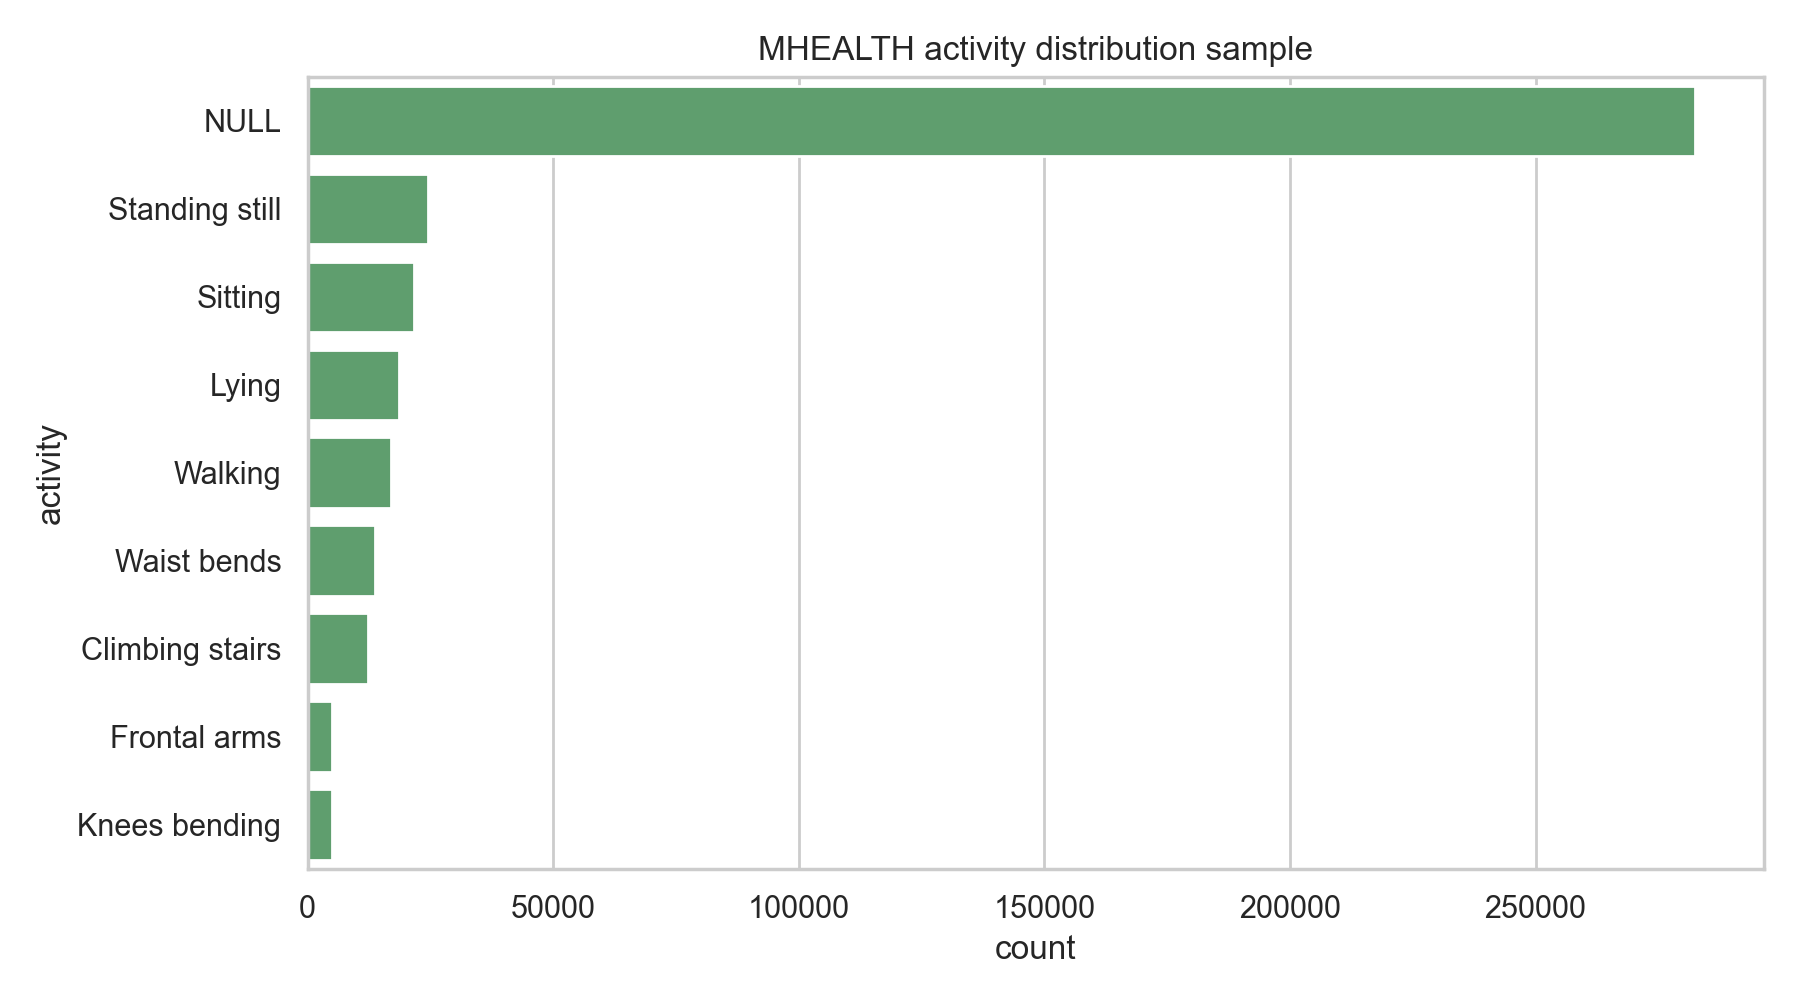
\includegraphics[width=\textwidth]{images/ch3/mhealth_activity_distribution.png}\caption{Python -- Activity distribution}\end{subfigure}
\caption[Phân bố hoạt động MHEALTH]{Tần suất hoạt động trong mẫu MHEALTH.\
\footnotesize Python source: \texttt{src/analyze\_mhealth.py}.\
}\label{fig:ch4_mhealth_activity}
\end{figure}
\textbf{Nhận xét Hình \ref{fig:ch4_mhealth_activity}.} Lớp NULL chiếm tỷ lệ lớn do nhiều đoạn không gán hoạt động; phân tích mô hình nên cân nhắc lọc NULL hoặc dùng class weight.

\begin{figure}[H]\centering
\begin{subfigure}{0.90\textwidth}\centering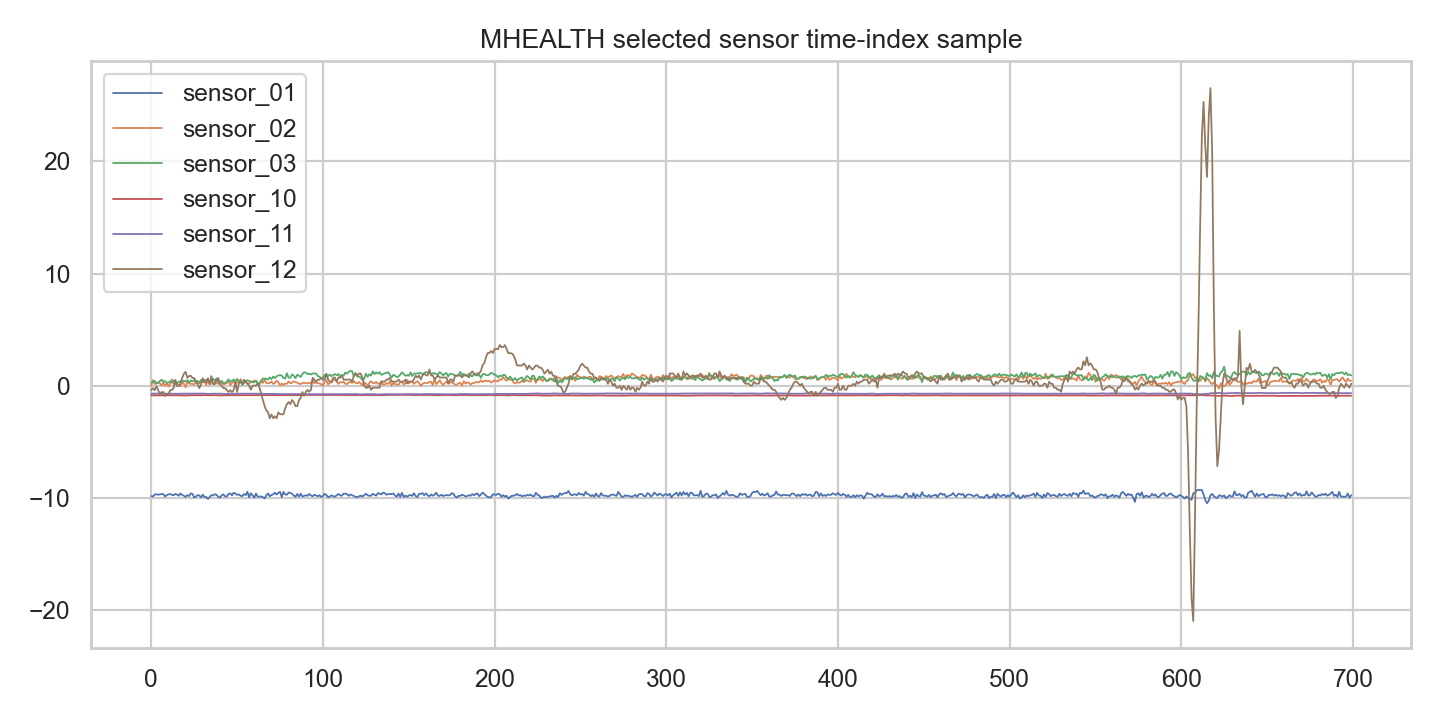
\includegraphics[width=\textwidth]{images/ch3/mhealth_selected_sensor_line.png}\caption{Python -- Sensor line sample}\end{subfigure}
\caption[Line chart MHEALTH]{Line chart theo index mẫu của 6 sensor MHEALTH.\
\footnotesize Python source: \texttt{scripts/generate\_group\_b\_figures.py}.\
}\label{fig:ch4_mhealth_line}
\end{figure}
\textbf{Nhận xét Hình \ref{fig:ch4_mhealth_line}.} Chuỗi sensor có dao động ngắn hạn mạnh, phản ánh chuyển động cơ thể. Biểu đồ đường phù hợp hơn histogram khi cần đọc đoạn hoạt động liên tiếp.

\begin{figure}[H]\centering
\begin{subfigure}{0.90\textwidth}\centering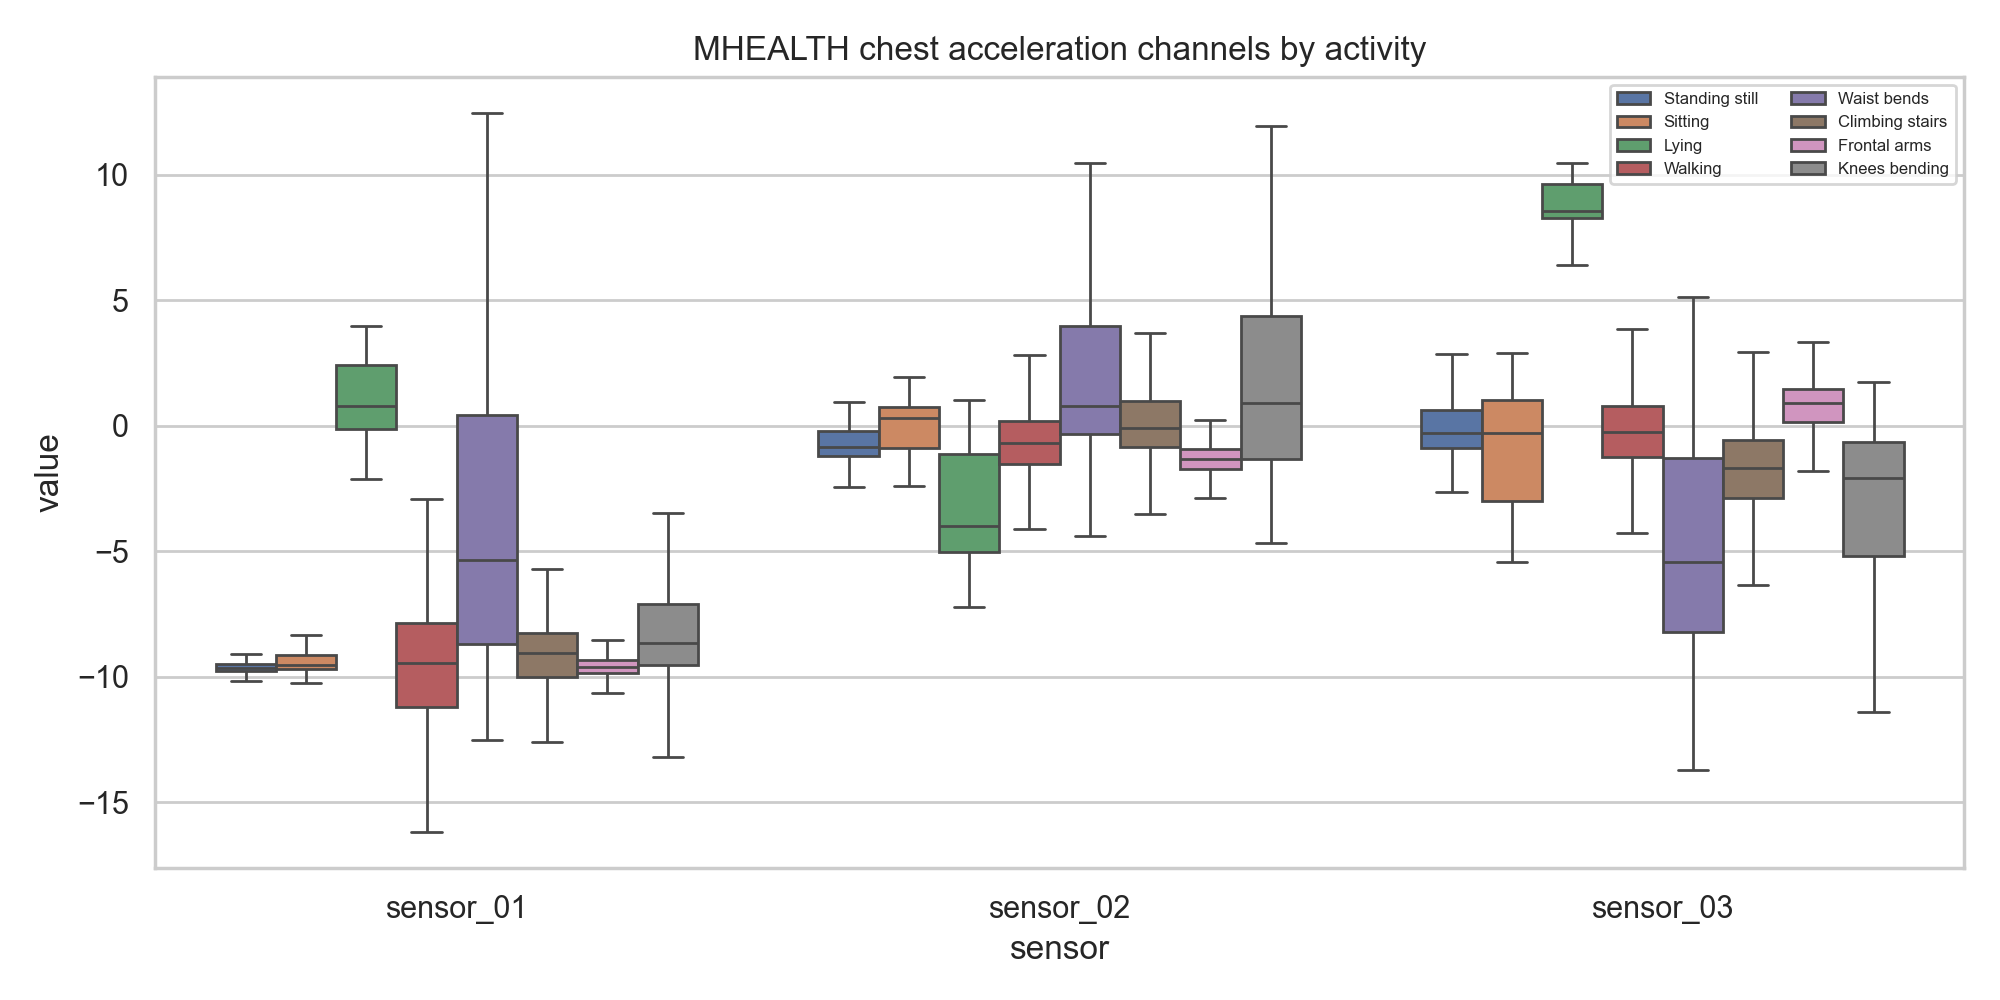
\includegraphics[width=\textwidth]{images/ch3/mhealth_sensor_boxplot.png}\caption{Python -- Sensor boxplot}\end{subfigure}
\caption[Boxplot MHEALTH]{Boxplot sensor theo hoạt động MHEALTH.\
\footnotesize Python source: \texttt{src/analyze\_mhealth.py}.\
}\label{fig:ch4_mhealth_box}
\end{figure}
\textbf{Nhận xét Hình \ref{fig:ch4_mhealth_box}.} Phân bố sensor khác nhau giữa các hoạt động; ngoại lai có thể là chuyển động đột ngột nên cần kiểm tra theo ngữ cảnh trước khi clipping.

\begin{figure}[H]\centering
\begin{subfigure}{0.90\textwidth}\centering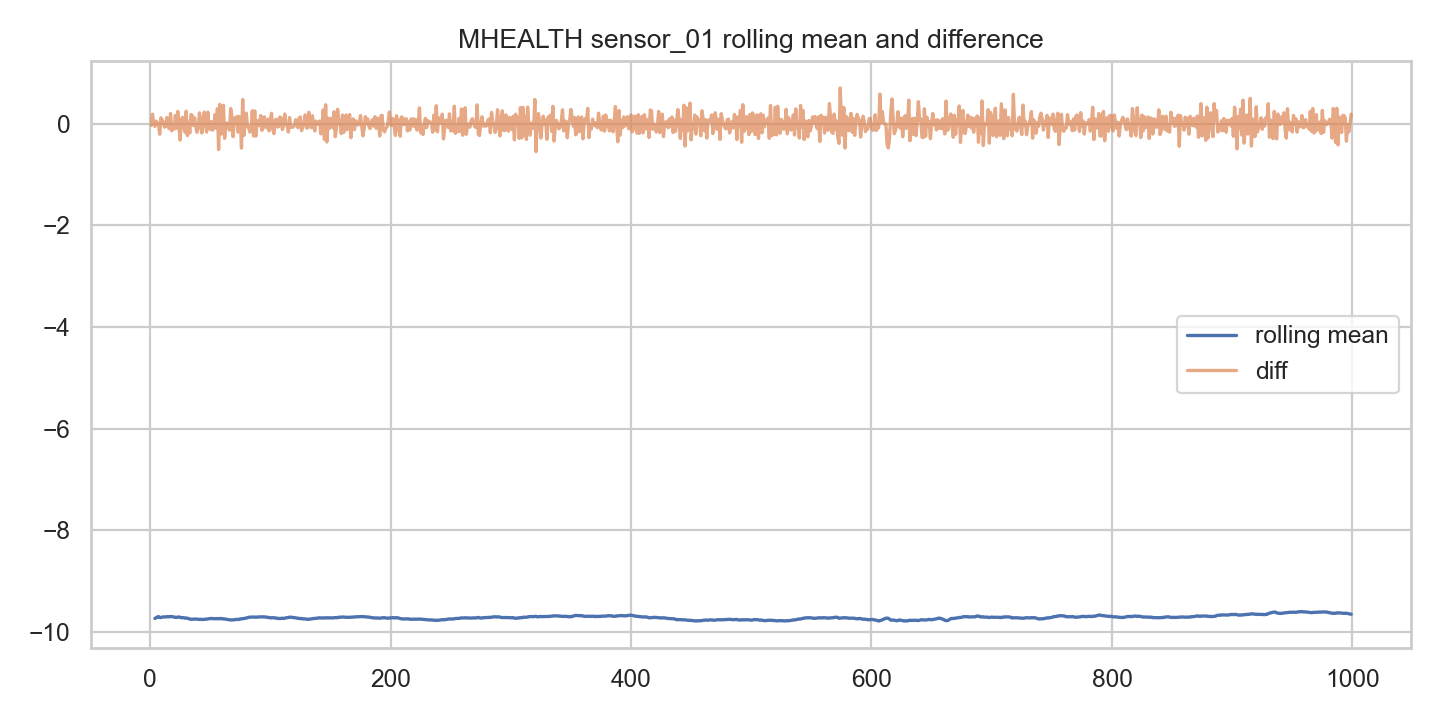
\includegraphics[width=\textwidth]{images/ch3/mhealth_sensor_rolling_diff.png}\caption{Python -- Rolling/differencing}\end{subfigure}
\caption[Rolling và differencing MHEALTH]{Rolling mean và sai phân của \texttt{sensor\_01}.\
\footnotesize Python source: \texttt{scripts/generate\_group\_b\_figures.py}.\
}\label{fig:ch4_mhealth_roll_diff}
\end{figure}
\textbf{Nhận xét Hình \ref{fig:ch4_mhealth_roll_diff}.} Rolling mean làm rõ mức nền của cảm biến, còn differencing nhấn mạnh thay đổi tức thời; hai cách nhìn này bổ sung cho phân tích hoạt động.

\begin{figure}[H]\centering
\begin{subfigure}{0.90\textwidth}\centering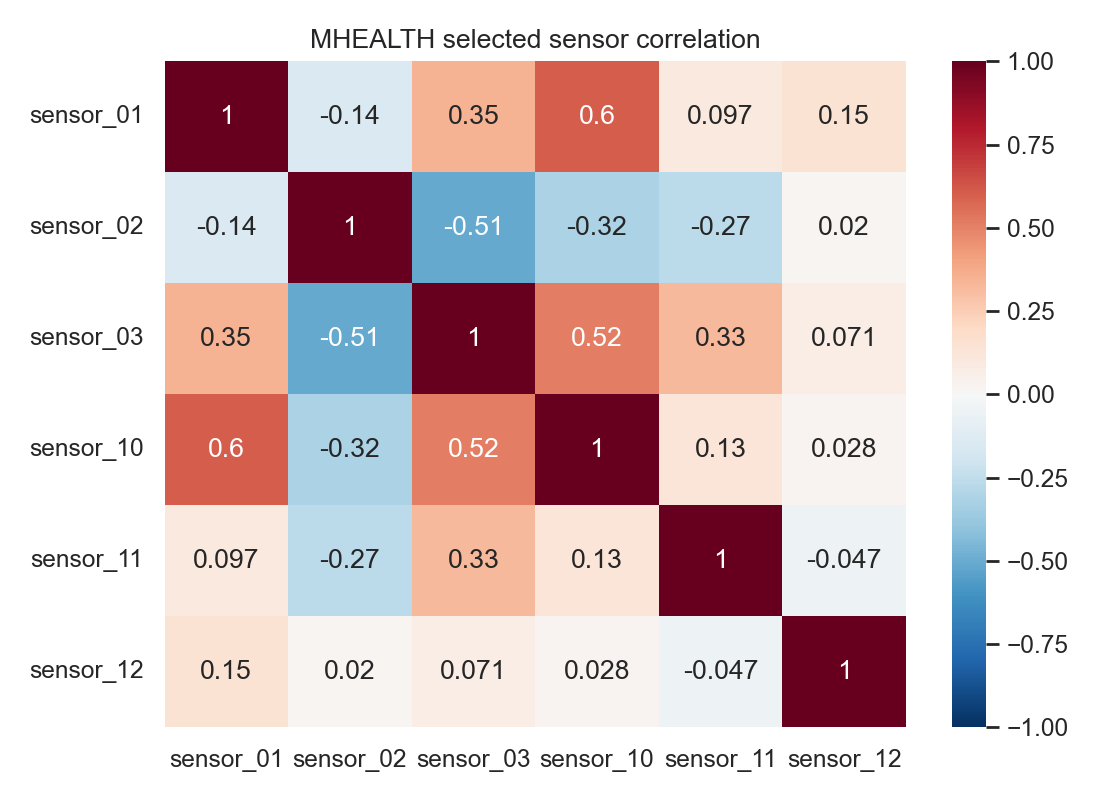
\includegraphics[width=\textwidth]{images/ch3/mhealth_sensor_correlation_heatmap.png}\caption{Python -- Correlation heatmap}\end{subfigure}
\caption[Heatmap MHEALTH]{Heatmap tương quan các sensor MHEALTH đã chọn.\
\footnotesize Python source: \texttt{scripts/generate\_group\_b\_figures.py}.\
}\label{fig:ch4_mhealth_corr}
\end{figure}
\textbf{Nhận xét Hình \ref{fig:ch4_mhealth_corr}.} Tương quan giữa các sensor cho biết mức trùng lặp thông tin giữa kênh đo; các kênh ít tương quan nên được giữ lại để mô hình nhận diện chuyển động đa chiều.

\textbf{Bước 4. So sánh trước--sau.} Tương tự HAR, MHEALTH không có khuyết thiếu và các ngoại lai mang ý nghĩa chuyển động, nên ``trạng thái thô'' và ``trạng thái sạch'' gần như trùng nhau ở cấp độ giá trị. Phép biến đổi có giá trị nhất là \emph{rolling mean} (làm rõ mức nền cảm biến) và \emph{differencing} (nhấn mạnh thay đổi tức thời) trong Hình~\ref{fig:ch4_mhealth_roll_diff}: nếu coi chuỗi rolling/diff là ``trạng thái đã biến đổi'', thì nó tách bạch thành phần xu hướng và thành phần dao động ngắn hạn -- hữu ích cho nhận dạng hoạt động. Bài học là dữ liệu cảm biến chất lượng cao sẵn sàng cho mô hình, và việc biến đổi chuỗi (chứ không phải điền khuyết) mới là công cụ chính của Nhóm~B.

\chapterThreeExcelPythonComparison

\section{Số hóa, thống kê và trực quan hóa dữ liệu đa phương tiện}

Quy tắc cốt lõi của nhóm C là dữ liệu thô không thể đưa trực tiếp vào bảng thống kê. Ảnh, văn bản, âm thanh hoặc video phải được chuyển thành đặc trưng Quantitative trước: kích thước, cường độ pixel, độ dài văn bản, số ký tự, topic, TF-IDF, RMS energy, motion intensity, v.v. Dự án này chọn hai bộ dữ liệu nhóm C: HAM10000 (ảnh) và Reuters-21578 (văn bản).

\subsection{Bộ dữ liệu ảnh: HAM10000}

HAM10000 gồm 10\,015 ảnh da liễu cùng metadata chẩn đoán. Trong phân tích thống kê, ảnh được số hóa thành các biến \texttt{width}, \texttt{height}, \texttt{mean\_intensity}, \texttt{std\_intensity}, kết hợp với metadata \texttt{age}, \texttt{sex}, \texttt{localization}, \texttt{dx}.

\begin{table}[H]
\centering
\caption{Phân loại biến số hóa từ HAM10000}
\label{tab:ch4_ham_variable_types}
\small
\begin{tabularx}{\textwidth}{p{0.30\textwidth}p{0.32\textwidth}Y}
\toprule
Loại biến & Ví dụ & Ý nghĩa phân tích \\
\midrule
Quantitative Continuous & \texttt{mean\_intensity}, \texttt{std\_intensity} & Độ sáng, độ tương phản, mức phân tán sắc độ \\
Quantitative Discrete & \texttt{width}, \texttt{height}, tổng số pixel & Kích thước hình học của ảnh \\
Qualitative & \texttt{dx}, \texttt{dx\_type}, \texttt{localization}, \texttt{sex} & Nhãn chẩn đoán và metadata \\
\bottomrule
\end{tabularx}
\end{table}

\begin{table}[H]
\centering
\caption[Thống kê đặc trưng ảnh HAM10000]{Thống kê đặc trưng ảnh HAM10000. Source: \texttt{outputs/tables/ham10000\_numeric\_summary.csv}.}
\label{tab:ch4_ham_stats}
\scriptsize
\setlength{\tabcolsep}{4pt}
\begin{tabular}{lrrrrrrrr}
\toprule
Biến & Mean & Median & Std & Min & Max & CV & IQR & n \\
\midrule
\texttt{width} & 600.00 & 600.00 & 0.00 & 600 & 600 & 0.000 & 0.00 & 1000 \\
\texttt{height} & 450.00 & 450.00 & 0.00 & 450 & 450 & 0.000 & 0.00 & 1000 \\
\texttt{mean\_intensity} & 156.73 & 156.93 & 18.94 & 93.88 & 215.91 & 0.121 & 25.05 & 1000 \\
\texttt{std\_intensity} & 27.97 & 25.83 & 11.37 & 6.46 & 73.23 & 0.407 & 14.16 & 1000 \\
\texttt{age} & 53.08 & 50.00 & 16.75 & 0 & 85 & 0.316 & 25.00 & 990 \\
\bottomrule
\end{tabular}
\end{table}

\begin{figure}[H]
\centering
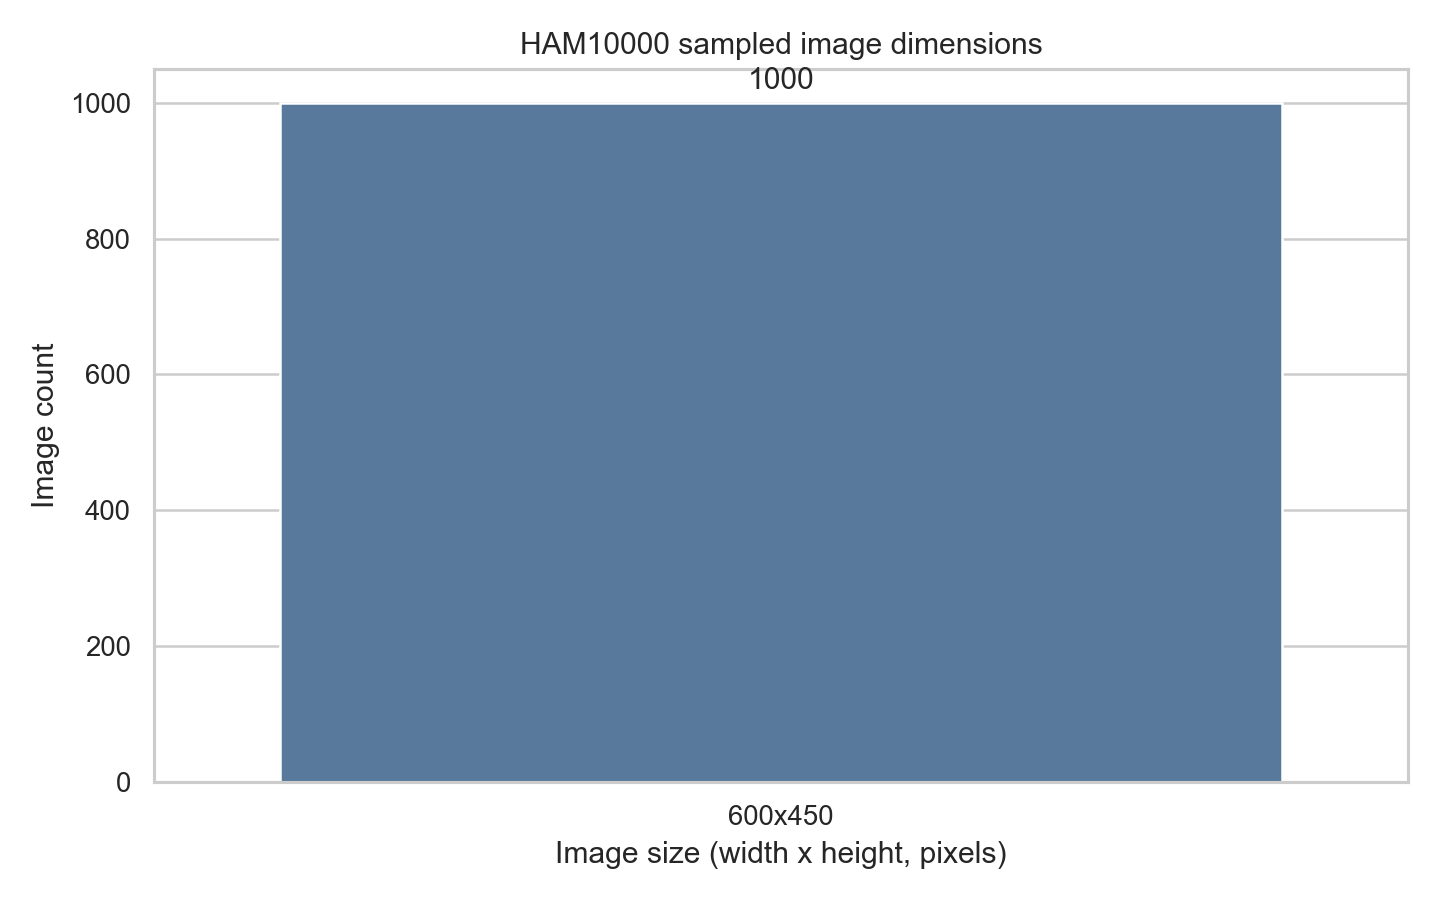
\includegraphics[width=0.94\textwidth]{images/ch3/ham10000_image_dimensions_histogram.png}
\caption[Histogram kích thước ảnh HAM10000]{Histogram kích thước ảnh HAM10000. Python source: \texttt{src/analyze\_ham10000.py}.}
\label{fig:ch4_ham_dimensions}
\end{figure}

\textbf{Nhận xét Hình \ref{fig:ch4_ham_dimensions}.} Kích thước ảnh gần như đồng nhất ở 600$\times$450, nên biến \texttt{width} và \texttt{height} chủ yếu dùng để xác nhận chất lượng dữ liệu đầu vào hơn là tạo thông tin phân biệt lớp.

\begin{figure}[H]
\centering
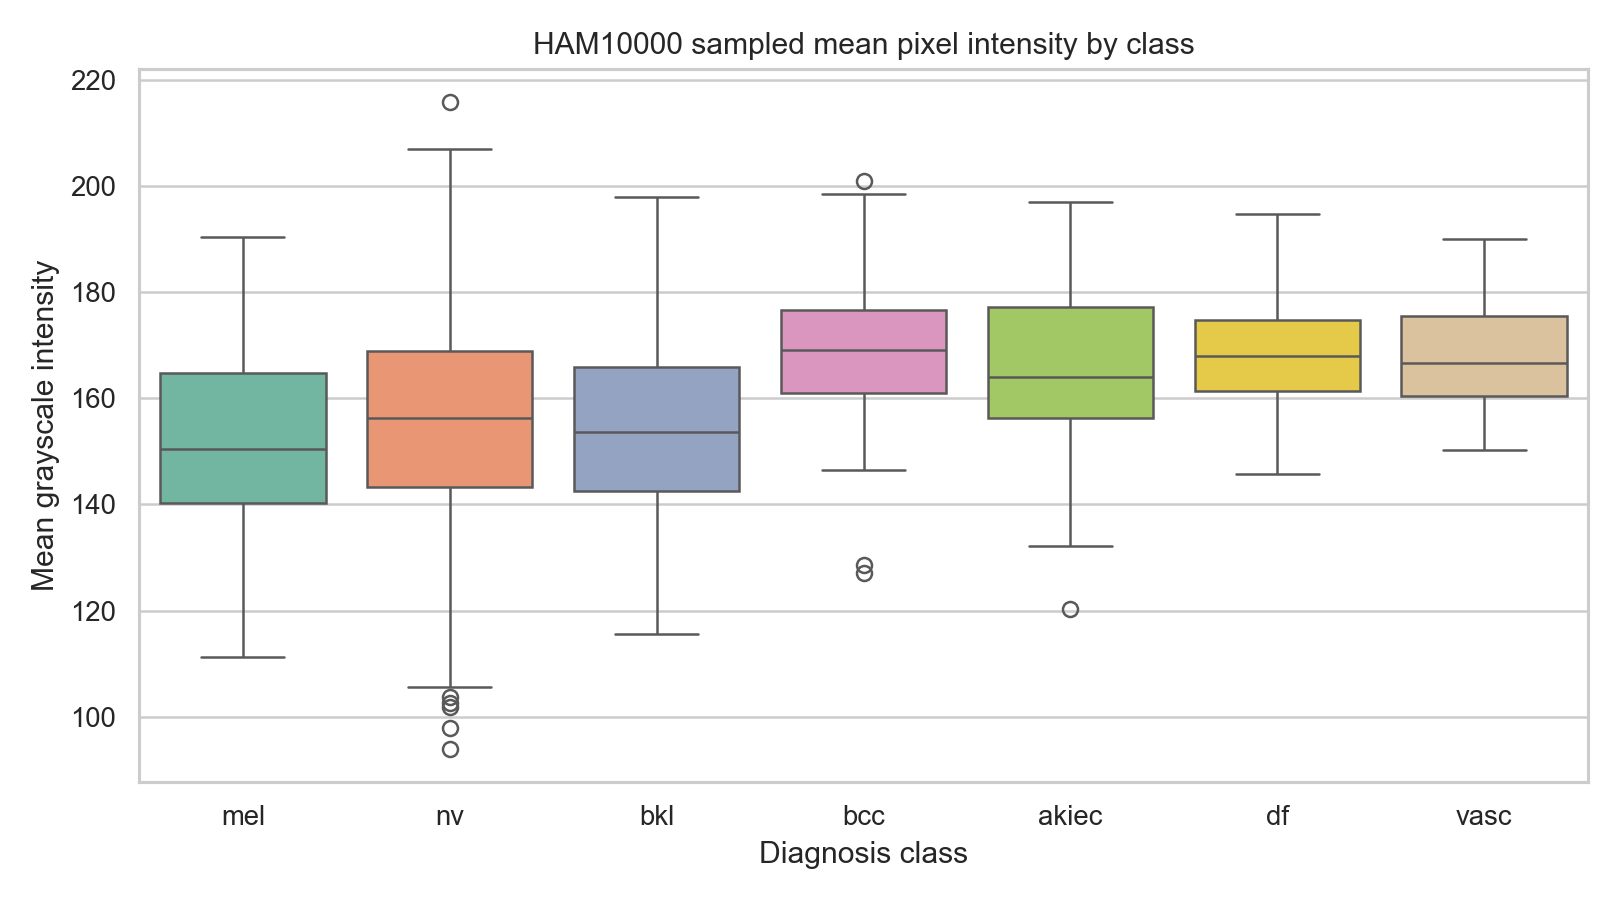
\includegraphics[width=0.94\textwidth]{images/ch3/ham10000_mean_intensity_boxplot.png}
\caption[Boxplot độ sáng theo lớp HAM10000]{Boxplot \texttt{mean\_intensity} theo lớp chẩn đoán HAM10000. Python source: \texttt{src/analyze\_ham10000.py}.}
\label{fig:ch4_ham_intensity}
\end{figure}

\textbf{Nhận xét Hình \ref{fig:ch4_ham_intensity}.} Boxplot độ sáng theo lớp cho thấy có chồng lấn lớn giữa các nhóm chẩn đoán. Vì vậy, đặc trưng thống kê ảnh đơn giản như \texttt{mean\_intensity} và \texttt{std\_intensity} chỉ nên xem là bước mô tả, không đủ thay thế đặc trưng màu/texture hoặc transfer learning.

\begin{figure}[H]
\centering
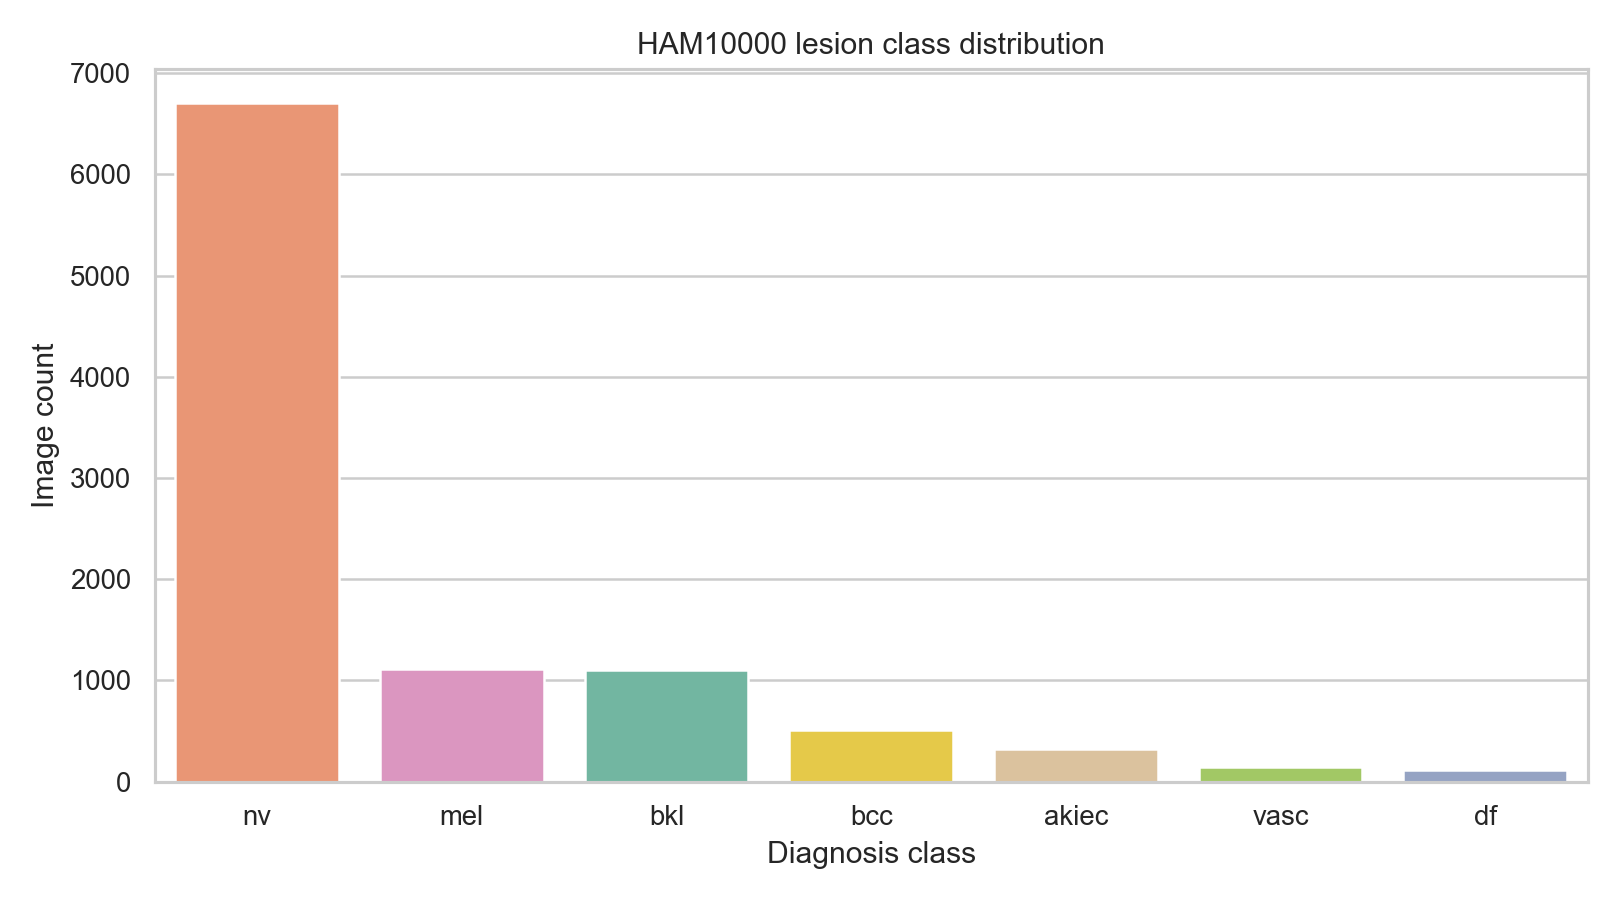
\includegraphics[width=0.94\textwidth]{images/ch3/ham10000_class_distribution.png}
\caption[Phân bố lớp \texttt{dx} HAM10000]{Phân bố lớp chẩn đoán \texttt{dx} trong HAM10000. Python source: \texttt{src/analyze\_ham10000.py}.}
\label{fig:ch4_ham_class_distribution}
\end{figure}

\textbf{Nhận xét Hình \ref{fig:ch4_ham_class_distribution}.} Phân bố lớp \texttt{dx} mất cân bằng mạnh, đặc biệt lớp \texttt{nv} chiếm tỷ trọng lớn. Vì vậy, accuracy có thể đánh lừa nếu mô hình chỉ dự đoán lớp phổ biến; khi đánh giá phân loại ảnh cần đọc thêm macro-F1, recall theo lớp và ma trận nhầm lẫn.

\begin{figure}[H]
\centering
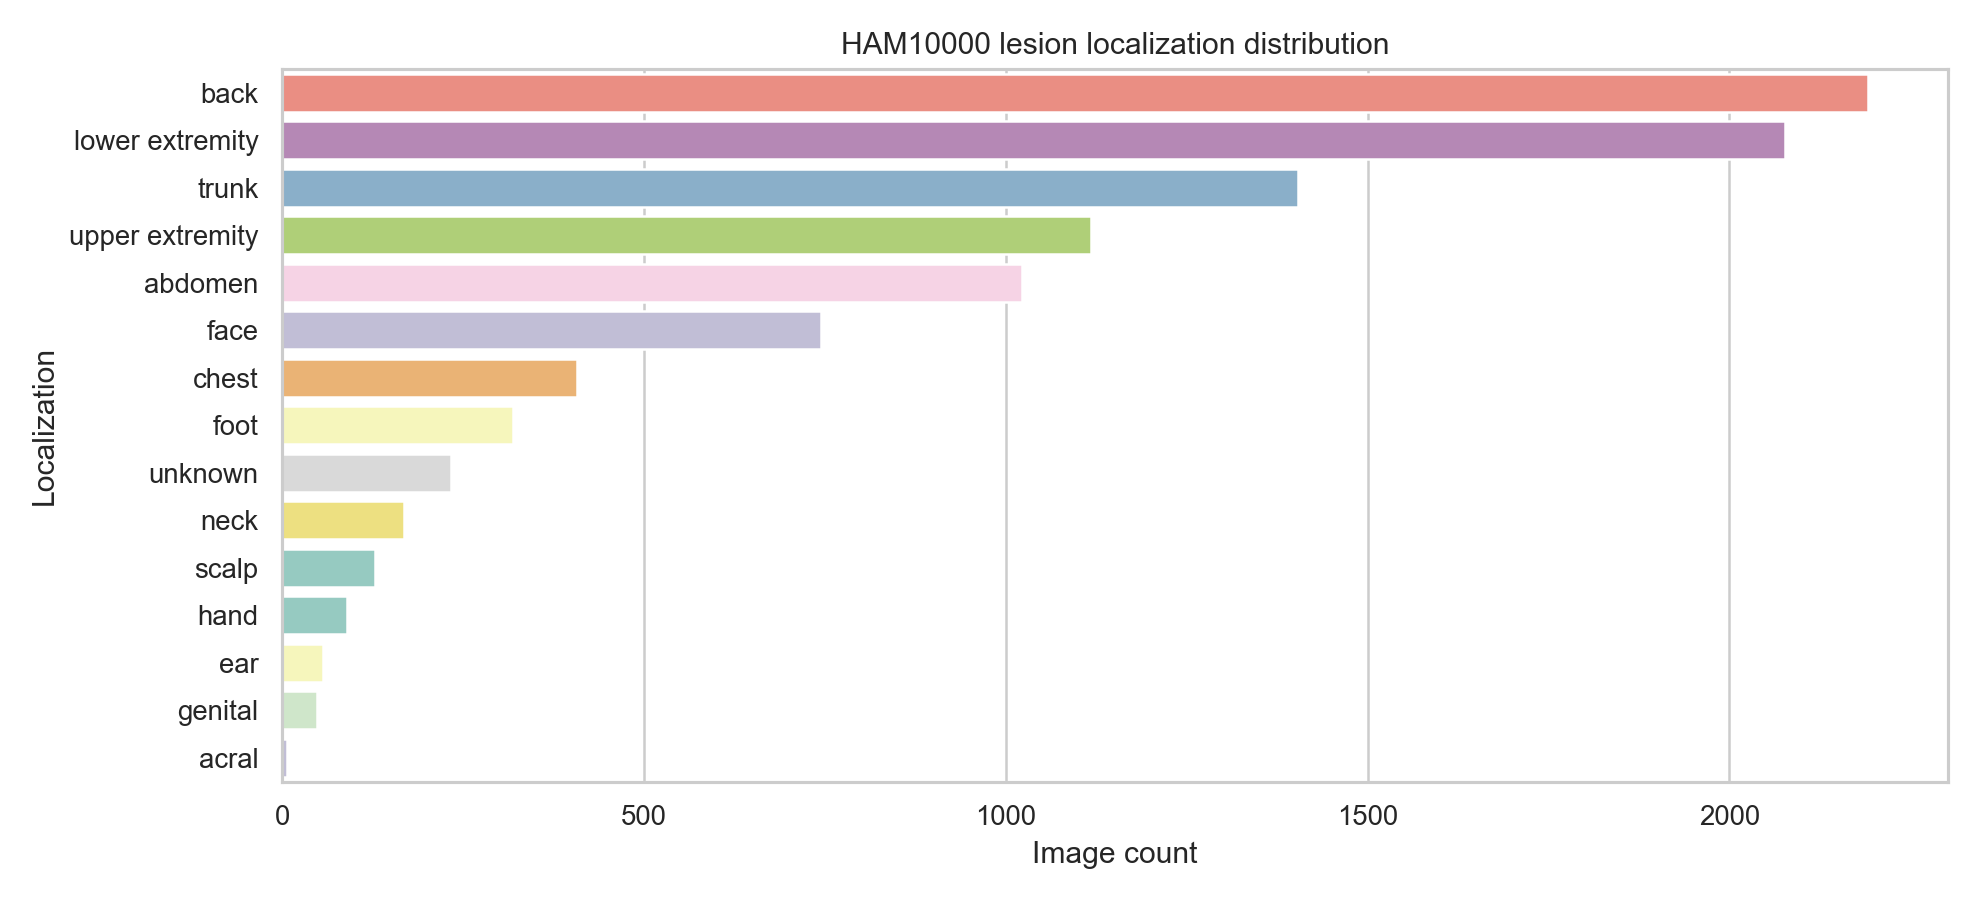
\includegraphics[width=0.94\textwidth]{images/ch3/ham10000_localization_bar.png}
\caption[Vị trí tổn thương HAM10000]{Tần suất vị trí tổn thương trong metadata HAM10000. Python source: \texttt{src/analyze\_ham10000.py}.}
\label{fig:ch4_ham_localization}
\end{figure}

\textbf{Nhận xét Hình \ref{fig:ch4_ham_localization}.} Biểu đồ vị trí tổn thương cho thấy một số vùng cơ thể xuất hiện nhiều hơn, nhưng vị trí không đủ để thay thế thông tin ảnh vì nhiều lớp bệnh có thể cùng xuất hiện ở một vùng.

\begin{figure}[H]
\centering
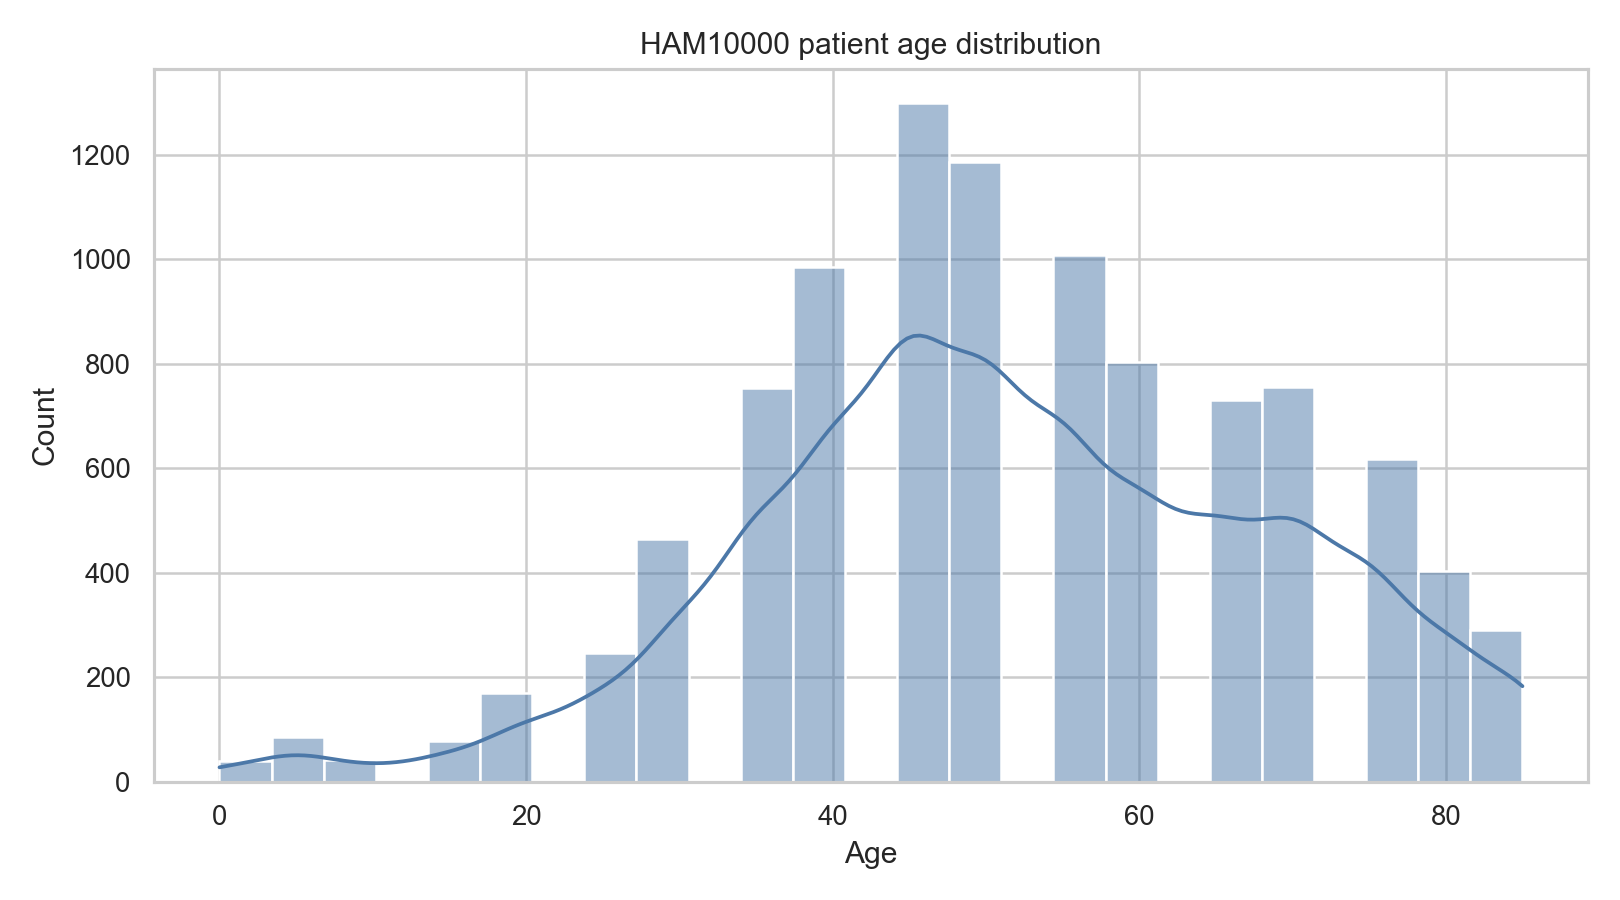
\includegraphics[width=0.78\textwidth]{images/ch3/ham10000_age_histogram.png}
\caption[Phân phối tuổi bệnh nhân HAM10000]{Phân phối tuổi bệnh nhân trong metadata HAM10000. Python source: \texttt{src/analyze\_ham10000.py}.}
\label{fig:ch4_ham_age}
\end{figure}

\textbf{Nhận xét Hình \ref{fig:ch4_ham_age}.} Histogram tuổi cho thấy mẫu HAM10000 tập trung nhiều ở nhóm trung niên và lớn tuổi, phù hợp với bối cảnh bệnh da liễu thường được ghi nhận nhiều hơn ở nhóm tuổi cao. Khi dùng metadata cho mô hình, tuổi có thể là biến hỗ trợ, nhưng không nên thay thế thông tin ảnh vì cùng một độ tuổi vẫn có thể xuất hiện nhiều lớp chẩn đoán khác nhau.

\textbf{Nhận xét tổng hợp HAM10000.} Kích thước ảnh đồng nhất ở 600$\times$450 nên không cần xử lý resize khi thống kê hình học. \texttt{mean\_intensity} dao động từ 93.88 đến 215.91, cho thấy sắc độ ảnh có đủ biến thiên để dùng làm đặc trưng mô tả. Tuy nhiên, các đặc trưng cường độ pixel đơn lẻ không đủ để phân loại ổn định, mà cần kết hợp đặc trưng sâu hoặc mô hình ảnh ở phần học máy.

\subsection{Bộ dữ liệu văn bản: Reuters-21578}

Reuters-21578 gồm 21\,578 văn bản tin tức. Văn bản được số hóa thành \texttt{word\_count}, \texttt{char\_count}, \texttt{primary\_topic} và danh sách topic đa nhãn. Các đặc trưng nâng cao như TF-IDF có thể dùng ở chương học máy, còn chương này tập trung vào thống kê độ dài và phân bố topic.

\begin{table}[H]
\centering
\caption{Phân loại biến số hóa từ Reuters-21578}
\label{tab:ch4_reuters_variable_types}
\small
\begin{tabularx}{\textwidth}{p{0.30\textwidth}p{0.32\textwidth}Y}
\toprule
Loại biến & Ví dụ & Ý nghĩa phân tích \\
\midrule
Quantitative Continuous & Điểm cảm xúc, mật độ stop words & Đặc trưng ngữ nghĩa mở rộng \\
Quantitative Discrete & \texttt{word\_count}, \texttt{char\_count}, số câu & Độ dài và độ phức tạp văn bản \\
Qualitative & \texttt{primary\_topic}, \texttt{topics}, ngôn ngữ & Nhãn phân loại chủ đề \\
\bottomrule
\end{tabularx}
\end{table}

\begin{table}[H]
\centering
\caption[Thống kê đặc trưng văn bản Reuters-21578]{Thống kê đặc trưng văn bản Reuters-21578. Source: \texttt{outputs/tables/reuters\_text\_summary.csv}.}
\label{tab:ch4_reuters_stats}
\small
\begin{tabular}{lrrrrrrrr}
\toprule
Biến & Mean & Median & Std & Min & Max & CV & IQR & n \\
\midrule
\texttt{word\_count} & 132.86 & 93.00 & 139.70 & 0 & 2\,381 & 1.051 & 111 & 21\,578 \\
\texttt{char\_count} & 762.06 & 534.00 & 819.74 & 0 & 9\,910 & 1.076 & 672 & 21\,578 \\
\bottomrule
\end{tabular}
\end{table}

\begin{figure}[H]
\centering
\begin{subfigure}{0.48\textwidth}
 \centering
 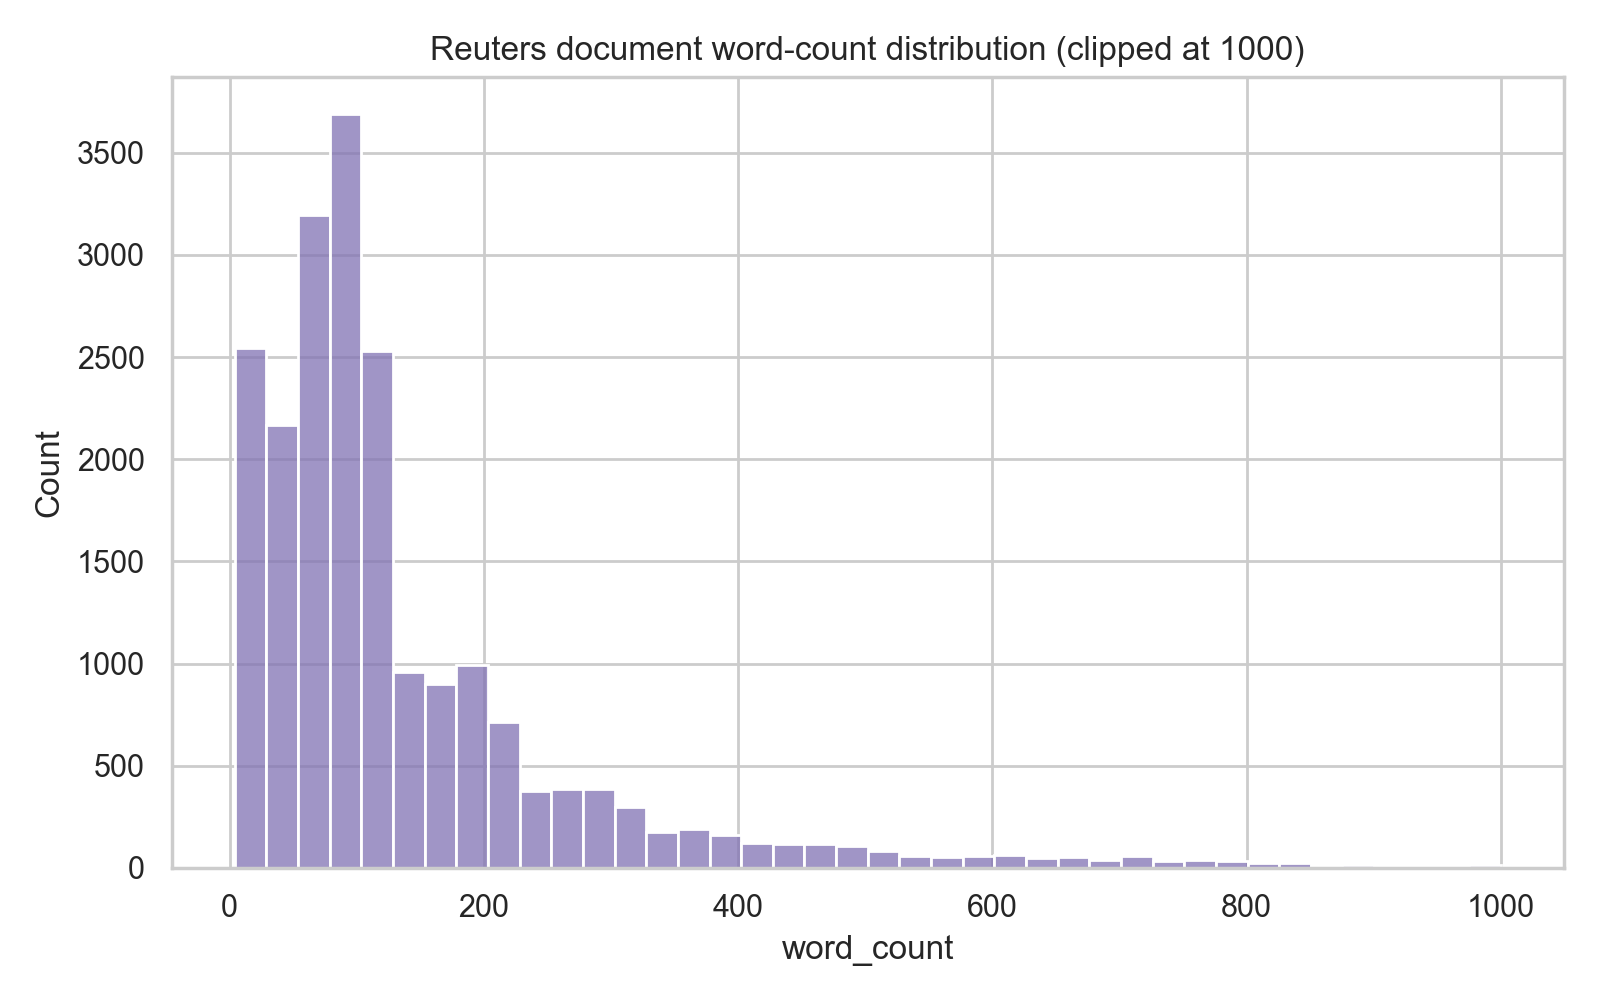
\includegraphics[width=\textwidth]{images/ch3/reuters_word_count_histogram.png}
 \caption{Histogram số từ}
\end{subfigure}
\hfill
\begin{subfigure}{0.48\textwidth}
 \centering
 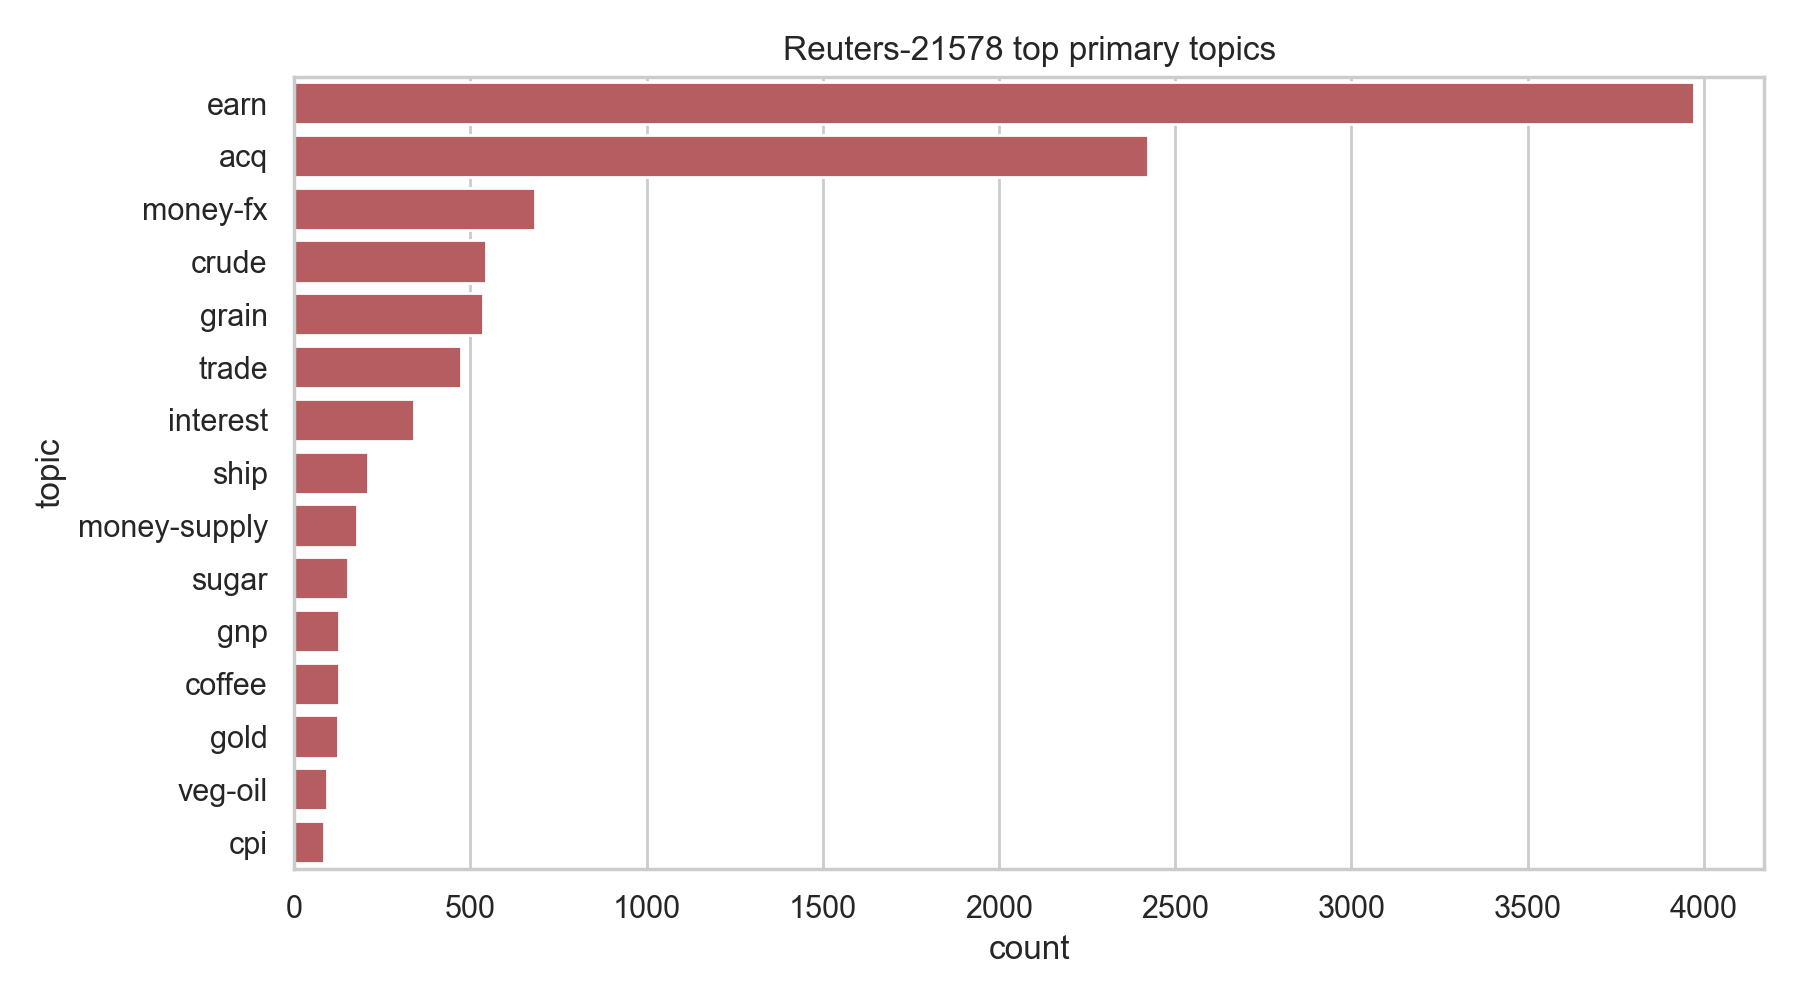
\includegraphics[width=\textwidth]{images/ch3/reuters_top_topics.png}
 \caption{Top topic}
\end{subfigure}
\caption[Số hóa văn bản Reuters-21578]{Số hóa và trực quan hóa văn bản Reuters-21578. Python source: \texttt{src/analyze\_reuters.py}.}
\label{fig:ch4_reuters_dataset}
\end{figure}

\textbf{Nhận xét Hình \ref{fig:ch4_reuters_dataset}.} Histogram \texttt{word\_count} cho thấy phân phối lệch phải rất mạnh: đa số tin ngắn, một số ít tin rất dài. Biểu đồ top topic cho thấy \texttt{earn} và \texttt{acq} chiếm ưu thế, trong khi nhiều topic chuyên ngành có ít mẫu; khi dùng Reuters cho phân loại văn bản, macro-F1 sẽ có ý nghĩa hơn accuracy vì phản ánh tốt hơn hiệu năng trên các lớp nhỏ.

\begin{figure}[H]
\centering
\begin{subfigure}{0.48\textwidth}
 \centering
 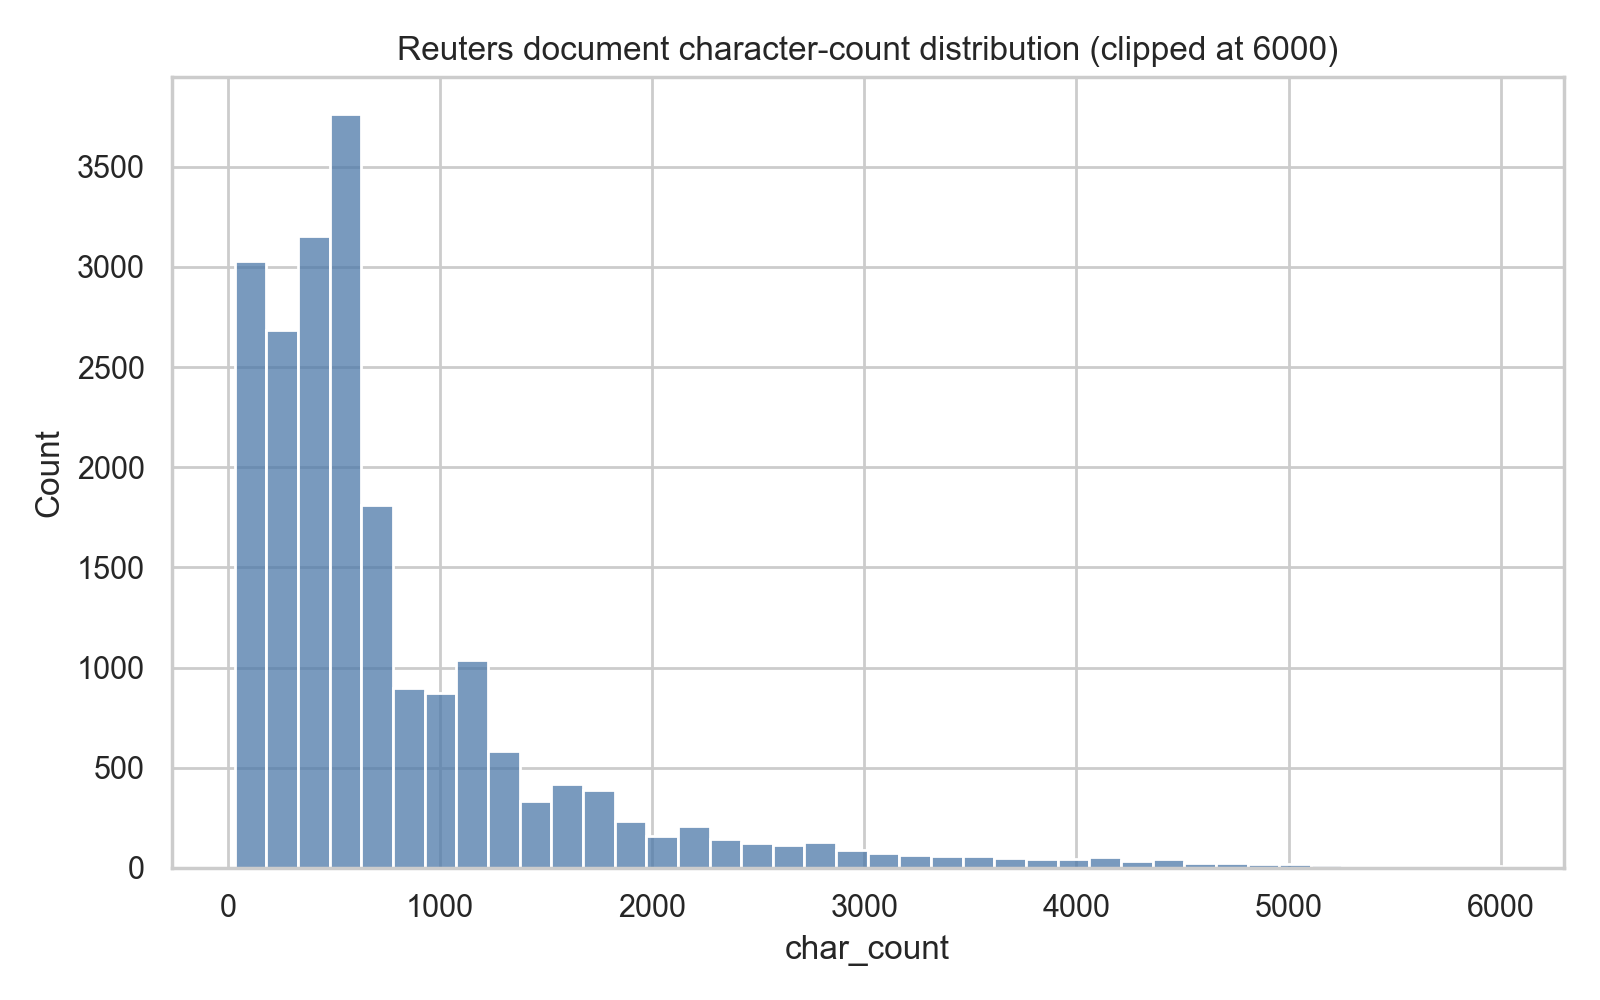
\includegraphics[width=\textwidth]{images/ch3/reuters_char_count_histogram.png}
 \caption{Histogram số ký tự}
\end{subfigure}
\hfill
\begin{subfigure}{0.48\textwidth}
 \centering
 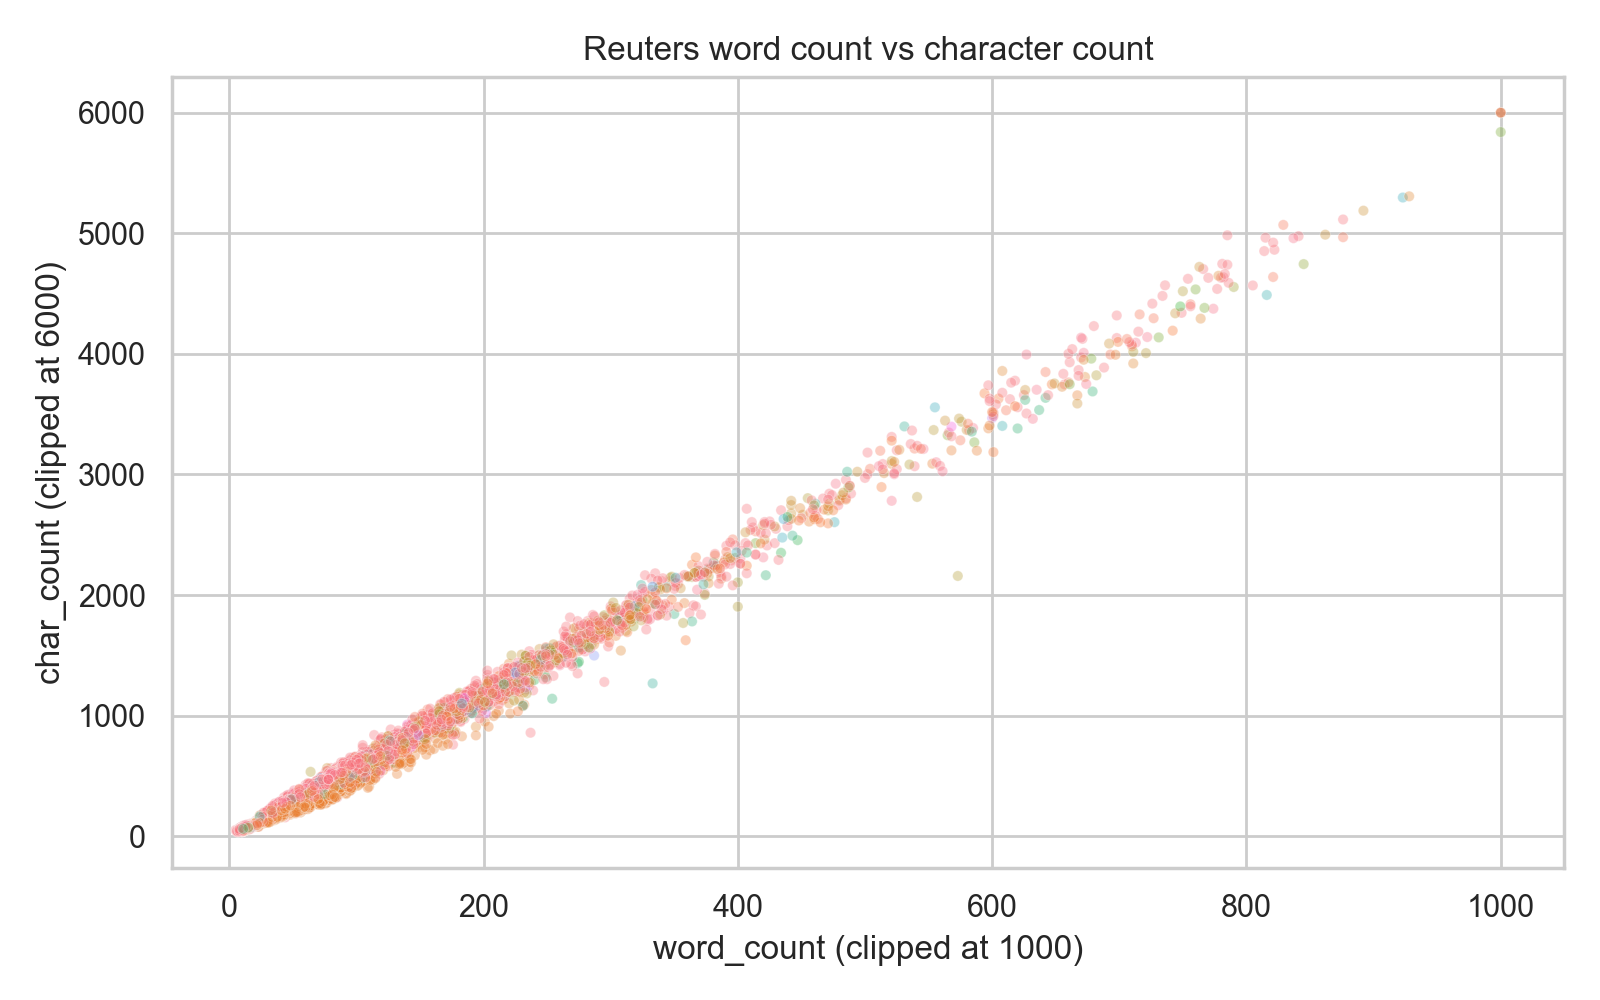
\includegraphics[width=\textwidth]{images/ch3/reuters_word_char_scatter.png}
 \caption{Scatter số từ--số ký tự}
\end{subfigure}
\caption[Phân tích độ dài văn bản Reuters-21578]{Phân tích độ dài văn bản Reuters-21578 theo số ký tự và quan hệ số từ--số ký tự. Python source: \texttt{src/analyze\_reuters.py}.}
\label{fig:ch4_reuters_length}
\end{figure}

\textbf{Nhận xét Hình \ref{fig:ch4_reuters_length}.} Histogram số ký tự xác nhận kết luận từ \texttt{word\_count}: phần lớn bản tin ngắn, nhưng vẫn có đuôi phải gồm các văn bản dài. Scatter số từ--số ký tự gần như tạo thành một dải tuyến tính, nghĩa là hai đặc trưng độ dài chứa thông tin trùng lặp đáng kể; khi xây dựng mô hình, nên chuẩn hóa hoặc chọn một đại diện độ dài để tránh làm mô hình quá thiên về kích thước văn bản thay vì nội dung.

\section{Kết luận chương}

Chương này đã triển khai đầy đủ yêu cầu thống kê và trực quan hóa trên ba nhóm dữ liệu. Với nhóm A, Heart Disease cho thấy vai trò của phân loại biến và xử lý ngoại lai; CDC Diabetes nhấn mạnh dữ liệu lớn, biến thứ bậc và mất cân bằng lớp; Breast Cancer thể hiện các biến Quantitative có lực phân tách rõ. Với nhóm B, Appliances Energy chứng minh cần đọc xu hướng bằng line chart và dùng log-transform cho phân phối lệch phải; HAR/MHEALTH cho thấy dữ liệu cảm biến cần chuẩn hóa trước khi tính khoảng cách hoặc gom cụm. Với nhóm C, HAM10000 và Reuters-21578 chứng minh nguyên tắc số hóa dữ liệu đa phương tiện thành đặc trưng Quantitative trước khi thống kê.

Các kết quả này là nền tảng trực tiếp cho chương học máy: phân loại nhóm A phải chú ý mất cân bằng và ngoại lai; dự báo nhóm B phải tách theo thời gian; gom cụm nhóm A/B/C phải chuẩn hóa đặc trưng và ẩn nhãn trước khi đánh giá cấu trúc tự nhiên của dữ liệu.
